\documentclass[11pt,openany]{book}
% ------------------------------------------------------------
% Preamble for 「銀河力学で学ぶ数値計算法」
% Style guide v1.1: A4, derivation-centered, restrained emphasis.
% Compile with XeLaTeX.
% ------------------------------------------------------------
\usepackage[a4paper,inner=27mm,outer=22mm,top=22mm,bottom=25mm,
  headheight=14pt,headsep=6mm]{geometry}

\usepackage{amsmath,amssymb,mathtools,bm}
\usepackage{graphicx,float,caption}
\captionsetup{font=small,labelfont=bf,labelsep=quad}
\graphicspath{{figures/}{./}}

\usepackage{fontspec}
\usepackage{xeCJK}
\IfFontExistsTF{Latin Modern Roman}{\setmainfont{Latin Modern Roman}}{\setmainfont{Liberation Serif}}
\IfFontExistsTF{Latin Modern Sans}{\setsansfont{Latin Modern Sans}}{\setsansfont{Liberation Sans}}
\IfFontExistsTF{DejaVu Sans Mono}{\setmonofont{DejaVu Sans Mono}[Scale=0.91]}{}
\setCJKmainfont{Noto Serif CJK JP}[ItalicFont={Noto Serif CJK JP}]
\setCJKsansfont{Noto Sans CJK JP}
\setCJKmonofont{Noto Sans Mono CJK JP}[Scale=0.90]
\xeCJKsetup{CJKmath=true}
\XeTeXlinebreaklocale "ja"
\XeTeXlinebreakskip = 0pt plus 0.1pt minus 0.01pt

\usepackage{xcolor,enumitem,array,booktabs,longtable,needspace,tabularx,xurl}
\usepackage{tikz}
\usetikzlibrary{arrows.meta,calc,positioning,patterns,decorations.pathreplacing,matrix}
\usepackage[most]{tcolorbox}
\usepackage{fancyvrb}
% Code blocks in Listing and Notebook excerpts use line numbers for discussion in class.
\fvset{numbers=left,numbersep=5pt,firstnumber=1,stepnumber=1}
\renewcommand{\theFancyVerbLine}{\sffamily\scriptsize\color{graytext}\arabic{FancyVerbLine}}
\usepackage{titlesec,fancyhdr}

\setlength{\parindent}{1em}
\setlength{\parskip}{0.15em}
\linespread{1.08}
\raggedbottom
\emergencystretch=1.5em
\widowpenalty=10000
\clubpenalty=10000

% --- Color system inherited from the simulation text, with restrained accents.
\definecolor{navy}{HTML}{0D1B3E}
\definecolor{cyan}{HTML}{1F6390}
\definecolor{cyanbg}{HTML}{E7F0F7}
\definecolor{turquoise}{HTML}{3A8F9B}
\definecolor{turquoisebg}{HTML}{EDF7F8}
\definecolor{amber}{HTML}{A8680B}
\definecolor{amberbg}{HTML}{FFF2CF}
\definecolor{rule}{HTML}{C9D2E3}
\definecolor{graytext}{HTML}{555555}
\definecolor{listingbg}{HTML}{F7F8FA}
\definecolor{listingframe}{HTML}{B8C0CC}

% --- Chapter-opening learning box: only full-width pedagogical box used routinely.
\newtcolorbox{learningbox}[1][本章で学ぶこと]{
  enhanced,breakable,
  colback=cyanbg,colframe=cyan,boxrule=0.65pt,arc=1.5pt,
  left=3mm,right=3mm,top=2.2mm,bottom=2.2mm,
  colbacktitle=cyan,coltitle=white,fonttitle=\sffamily\bfseries,
  title={#1},before skip=5pt,after skip=8pt}

% --- Kouya-inspired thin box: only for definitions/theorems with independent meaning.
\newtcolorbox{definitionbox}[2][]{
  enhanced,breakable,
  colback=white,colframe=turquoise,boxrule=0.6pt,arc=0pt,
  left=3mm,right=3mm,top=5.5mm,bottom=2.2mm,
  before skip=7pt,after skip=7pt,
  overlay unbroken and first={
    \node[anchor=north west,fill=turquoise,text=white,
      font=\sffamily\bfseries\small,inner xsep=2.2mm,inner ysep=0.8mm]
      at (frame.north west) {#2};
  },#1}

% --- Scoped supplements: white background + left rule only.
\newtcolorbox{notebookblock}[1]{
  enhanced,breakable,frame hidden,boxrule=0pt,arc=0pt,
  colback=white,borderline west={2.2pt}{0pt}{turquoise},
  left=3.2mm,right=3mm,top=5.3mm,bottom=2mm,
  before skip=8pt,after skip=8pt,
  title={Notebook #1},
  coltitle=turquoise,colbacktitle=white,
  fonttitle=\sffamily\bfseries\small,
  boxed title style={boxrule=0pt,frame hidden,colback=white},
  attach boxed title to top left={xshift=0mm,yshift=-0.5mm}}

\newtcolorbox{cautionblock}[1]{
  enhanced,frame hidden,boxrule=0pt,arc=0pt,
  colback=white,borderline west={2.2pt}{0pt}{amber},
  left=3.2mm,right=3mm,top=5.3mm,bottom=2mm,
  before skip=8pt,after skip=8pt,
  title={数値計算上の注意｜#1},
  coltitle=amber,colbacktitle=white,
  fonttitle=\sffamily\bfseries\small,
  boxed title style={boxrule=0pt,frame hidden,colback=white},
  attach boxed title to top left={xshift=0mm,yshift=-0.5mm}}

% 本編の理解には必須でない関連手法を、補足として紹介する。
% 白背景と青い左線のみ。長い補足は必要に応じてページをまたいで表示する。
\newtcolorbox{topicblock}[1]{
  enhanced,breakable,
  frame hidden,boxrule=0pt,arc=0pt,
  colback=white,borderline west={2.2pt}{0pt}{cyan},
  left=3.2mm,right=3mm,top=5.3mm,bottom=2mm,
  before skip=8pt,after skip=8pt,
  before upper={\setlength{\parindent}{1em}\indent},
  title={補足｜#1},
  coltitle=cyan,colbacktitle=white,
  fonttitle=\sffamily\bfseries\small,
  boxed title style={boxrule=0pt,frame hidden,colback=white},
  attach boxed title to top left={xshift=0mm,yshift=-0.5mm}}

% Short Python code bridging a derived formula and the complete Notebook.
\newtcolorbox{listingbox}[2][]{
  enhanced,
  colback=listingbg,colframe=listingframe,boxrule=0.45pt,arc=0pt,
  left=2.8mm,right=2.8mm,top=6mm,bottom=2.5mm,
  before skip=8pt,after skip=8pt,
  overlay unbroken and first={
    \node[anchor=north west,fill=white,text=navy,
      font=\sffamily\bfseries\small,inner xsep=2.0mm,inner ysep=0.7mm]
      at ([xshift=1.2mm]frame.north west) {Listing #2};
  },#1}


% Compact source syntax; rendered as the scoped Notebook block.
\newcommand{\notebooktag}[2]{%
  \begin{notebookblock}{#1}#2\end{notebookblock}}

\titleformat{\chapter}{\LARGE\bfseries\sffamily\color{navy}}{第\thechapter 章}{0.8em}{}
\titleformat{\section}{\large\bfseries\sffamily\color{navy}}{\thesection}{0.5em}{}
\titleformat{\subsection}{\normalsize\bfseries\sffamily\color{navy}}{}{0pt}{}
\titlespacing*{\chapter}{0pt}{0pt}{12pt}
\titlespacing*{\section}{0pt}{1.1em}{0.4em}
\titlespacing*{\subsection}{0pt}{0.75em}{0.25em}

\setlist[itemize]{leftmargin=1.7em,itemsep=0.15em,topsep=0.25em}
\setlist[enumerate]{leftmargin=2em,itemsep=0.15em,topsep=0.25em}
\setcounter{tocdepth}{1}
\setcounter{secnumdepth}{1}

\pagestyle{fancy}
\fancyhf{}
\fancyhead[L]{\scriptsize\sffamily 銀河力学で学ぶ数値計算法}
\fancyhead[R]{\scriptsize\sffamily\nouppercase{\leftmark}}
\makeatletter
\renewcommand{\chaptermark}[1]{\markboth{第\thechapter 章\enspace #1}{}}
\makeatother
\fancyfoot[R]{\small\thepage}
\fancypagestyle{plain}{
  \fancyhf{}\fancyfoot[R]{\small\thepage}\renewcommand{\headrulewidth}{0pt}}

\newcommand{\unit}[1]{\,\mathrm{#1}}
\newcommand{\dd}{\mathrm{d}}
\renewcommand{\contentsname}{目次}
\renewcommand{\figurename}{図}
\renewcommand{\tablename}{表}
\renewcommand{\bibname}{参考図書}
\renewcommand{\thefigure}{\thechapter.\arabic{figure}}
\renewcommand{\thetable}{\thechapter.\arabic{table}}
\renewcommand{\theequation}{\thechapter.\arabic{equation}}

\renewcommand{\topfraction}{0.95}
\renewcommand{\bottomfraction}{0.85}
\renewcommand{\textfraction}{0.05}
\renewcommand{\floatpagefraction}{0.85}
\setcounter{topnumber}{3}
\setcounter{totalnumber}{5}
\setlength{\textfloatsep}{10pt plus 3pt minus 2pt}
\setlength{\intextsep}{10pt plus 3pt minus 2pt}

\usepackage[unicode,colorlinks=true,linkcolor=cyan,citecolor=cyan,urlcolor=cyan]{hyperref}


\title{\Huge\bfseries\color{navy} 銀河力学で学ぶ数値計算法\\[4mm]\large\normalfont\sffamily 配布版 v1.3}
\author{馬場淳一（鹿児島大学・国立天文台）}
\date{\number\year 年\number\month 月\number\day 日}

\begin{document}
\let\cleardoublepage\clearpage
\frontmatter
\maketitle
\tableofcontents
\chapter*{はじめに}
\addcontentsline{toc}{chapter}{はじめに}
\markboth{はじめに}{}

本書は、宇宙流体シミュレーションや重力多体系シミュレーションに進む学部生が、数値計算法の基礎と検証の考え方を学ぶための準備教材である。
B. Ryden ``\textit{Celestial and Stellar Dynamics}'' (2025) の輪講と並行して用い、そこで学ぶ質量モデル・重力場・恒星軌道を数値計算の題材とする。
Ryden の物理内容の説明を置き換えるのではなく、その式から実際に数値を求め、誤差と収束を検証する方法を学ぶ。

宇宙流体・重力多体系シミュレーションでは、物理量の離散化、重力場の計算、時間積分などを組み合わせる。
本書では、それらを最初から同時に扱わず、単純な問題で一つずつ学ぶ。
本文では基本的な計算法と検証方法を扱い、脚注や補足では、今学んでいる計算が将来のシミュレーションのどの処理に相当するかを示す。

\section*{本書のねらい}

数値計算では、コードがエラーなく最後まで実行され、もっともらしい図が得られても、その答えが正しいとは限らない。
格子幅や時間刻みによる離散化誤差、丸め誤差、計算領域や境界条件の設定による誤差が、気づかないうちに結果に入り込むからである。
本書で最も身につけてほしいのは、個々の公式よりも、得られた数値解が信頼できるかを自分で確かめる習慣である。
そのために、本書では次の3つの確認を繰り返し行う。

\begin{itemize}
  \item \textbf{解析解との比較}：解析解が分かっている問題で、コードと数値計算法が正しく働くことを確かめる。
  \item \textbf{保存量による診断}：エネルギーや角運動量など、物理的に保存されるべき量がどの程度保たれているかを調べる。
  \item \textbf{分解能を変えた収束の確認}：格子幅や時間刻みを変えて計算し、答えが収束するか、誤差が期待どおりの次数で減るかを調べる。
\end{itemize}

実際の研究で解く問題の多くには解析解がない。
だからこそ、まず解析解のある問題で手法を検証し、そのうえで保存量と収束を組み合わせて結果を確かめることが重要になる。
また、誤差が見つかったときには、それが離散化、丸め誤差、有限の計算領域や境界条件、あるいは近似したモデルそのもののどれに由来するのかを区別して考える。

\section*{本書の構成}

本編は第1--3章で完結する。第1・2章では Ryden §6.4 の球対称系を題材に数値積分と有限差分法を学び、第3章では §7.1 の球対称ポテンシャル中の軌道を題材に時間積分法を学ぶ。
本編は球対称系のみを扱うが、付録A・B・Cは、それぞれ第1・2・3章で学んだ方法を軸対称系や非軸対称系へ広げる発展内容であり、関心に応じて選んでよい。また、連立一次方程式の解法を詳しく知りたい場合は、数値線形代数の補足である付録Dを参照してほしい。
各 Notebook は単独で先頭から実行でき、本文との対応表と実行順序を冒頭に示している。

{\footnotesize
\begin{center}
\setlength{\tabcolsep}{3.5pt}
\begin{tabularx}{\linewidth}{>{\raggedright\arraybackslash}p{0.14\linewidth}>{\raggedright\arraybackslash}p{0.16\linewidth}>{\raggedright\arraybackslash}p{0.27\linewidth}X}
\toprule
本書 & Rydenテキストとの対応 & 物理的な題材 & 本書で学ぶ数値計算法 \\
\midrule
第1章\newline Notebook 1 & §6.4\newline 特に §6.4.2--6.4.3 & Plummer・Hernquist・NFW などの球対称密度分布 & 数値積分、誤差、収束次数 \\
第2章\newline Notebook 2 & §6.4 & 球対称密度分布からポテンシャル・重力場を求める問題 & 1次元 Poisson 境界値問題、有限差分、数値微分 \\
第3章\newline Notebook 3 & §7.1 & 球対称ポテンシャル中の恒星軌道 & 常微分方程式の初期値問題、Euler 法、古典的4次 Runge--Kutta 法（RK4）、リープフロッグ法 \\
\midrule
付録A\newline Notebook A & §6.5 & 薄い軸対称円盤、指数円盤、Mestel 円盤、回転曲線 & 第1章の数値積分の応用、格子収束 \\
付録B\newline Notebook B & §6.5\newline & 軸対称密度・ポテンシャル、Miyamoto--Nagai モデル & 2次元有限差分、対称軸の処理、疎行列、格子収束 \\
付録C\newline Notebook C & §7.2--7.3 & 軸対称・非軸対称ポテンシャル、エピサイクル運動、box・loop 軌道 & 第3章の時間積分法の応用、保存量による検証 \\
付録D & 直接の対応なし & 第2章・付録Bで現れる連立一次方程式の背景 & Gauss の消去法、LU 分解、疎行列、Jacobi 法 \\
\bottomrule
\end{tabularx}
\end{center}
(注) 表の「Rydenテキストとの対応」は、主として物理的な題材の対応を示しており、Rydenテキストが有限差分法や Poisson 方程式の数値ソルバーを扱っているという意味ではない。
}

\section*{本書で扱う範囲}

本書で学ぶ数値計算法は、次の4つである。

\begin{itemize}
  \item \textbf{数値積分}（第1章、付録A）
  \item \textbf{数値微分}（第2章）
  \item \textbf{有限差分法による境界値問題の解法}（第2章、付録B）
  \item \textbf{初期値問題に対する時間積分法}（第3章、付録C）
\end{itemize}

一方、補間法そのもの（スプライン補間など）、非線形方程式の解法（Newton 法など）、固有値問題は扱わない。
連立一次方程式はライブラリのソルバーで解き、その基本的な考え方を付録Dで紹介するにとどめる。
また、流体の方程式のような偏微分方程式を実際に時間発展させる数値解法そのものは扱わない。
ただし、境界条件、陽的・陰的な時間積分、粒子の初期位置分布や重力計算、および宇宙流体計算で使われる2次・3次精度 Runge--Kutta 法（RK2・RK3）との関係は、脚注や補足で紹介する。
これらは今後の学習への案内であり、本書で新たに実装する数値実験ではない。
これらの内容をさらに学ぶ場合は、巻末の参考図書を参照してほしい。

\section*{次の学習に向けて}

本教材で扱った数値積分、数値微分、有限差分法、時間積分法は、宇宙流体シミュレーションや重力多体系シミュレーションで使われる数値計算法の基礎となる。
一方、実際のシミュレーションでは、保存則に基づく離散化、数値流束、重力場の効率的な計算、複数の物理過程の結合など、さらに多くの数値計算法を組み合わせる必要がある。
本教材のあとに学ぶ内容は、目的に応じて次のように選ぶとよい。

\begin{itemize}
  \item \textbf{宇宙流体シミュレーションへ進む場合：}
  福江純・和田桂一・梅村雅之『宇宙流体力学の基礎［改訂版］』\cite{fukue2022}では、宇宙流体の基礎方程式、自己重力流体、波動、衝撃波、流体不安定性などを通して、宇宙流体力学そのものの物理的な基礎を学ぶことができる。
  富阪幸治・花輪知幸・牧野淳一郎編『シミュレーション天文学』\cite{tomisaka2007}では、常微分方程式と偏微分方程式の数値解法から、流体力学・磁気流体力学、自己重力を含む流体計算までを、天文シミュレーションとの関係を意識しながら学ぶことができる。
  藤井孝藏・立川智章『Pythonで学ぶ流体力学の数値計算法』\cite{fujii2020}では、圧縮性流体の数値計算法を Python による実装とともに学ぶことができる。
  松本倫明・大須賀健・須佐元『輻射電磁流体シミュレーションの基礎』\cite{matsumoto}では、有限体積法、数値流束、SPH 法、磁気流体力学、輻射流体力学など、宇宙物理シミュレーションで用いられる数値計算法をより詳しく学ぶことができる。

  \item \textbf{重力多体系・銀河力学シミュレーションへ進む場合：}
  James Binney \& Scott Tremaine, ``\textit{Galactic Dynamics}''\cite{bt2008}では、銀河の重力場の表現、多重極展開、基底関数展開、$N$ 体計算における重力計算法などを詳しく学ぶことができる。
  富阪幸治・花輪知幸・牧野淳一郎編『シミュレーション天文学』\cite{tomisaka2007}では、無衝突系・衝突系の重力多体系計算を含め、天文シミュレーションにおける $N$ 体計算を広く学ぶことができる。
  より専門的には、
  Sverre J. Aarseth, ``\textit{Gravitational N-Body Simulations: Tools and Algorithms}''\cite{aarseth2003}では、直接重力計算、時間積分、近接遭遇、正則化、個別時間刻み、精度と計算効率など、重力 $N$ 体シミュレーションのアルゴリズムを体系的に学ぶことができる。特に、星団のような衝突系の計算を詳しく学ぶ際の参考になる。
  Walter Dehnen \& Justin I. Read, ``\textit{N-body simulations of gravitational dynamics}''\cite{dehnen2011}は、衝突系と無衝突系の両方について、重力 $N$ 体シミュレーションで用いられる代表的な数値手法を整理したレビューであり、重力多体系計算の全体像を把握するための参考になる。
\end{itemize}

これらの専門的な教科書やレビューを読むときにも、本教材で繰り返した解析解との比較、収束試験、保存量による診断、誤差の原因を区別する考え方は、そのまま役立つ。


\mainmatter
% Auto-generated from the distributed notebook. Do not hand-edit.
\newcommand{\choneMExactA}{\ensuremath{0.353553390593}}
\newcommand{\choneLeftNForty}{\ensuremath{0.346910451143}}
\newcommand{\choneMidNForty}{\ensuremath{0.353560298293}}
\newcommand{\choneTrapNForty}{\ensuremath{0.353539577216}}
\newcommand{\choneSimpsonNForty}{\ensuremath{0.353553401385}}
\newcommand{\choneLeftErrNForty}{\ensuremath{6.643\times 10^{-3}}}
\newcommand{\choneMidErrNForty}{\ensuremath{6.908\times 10^{-6}}}
\newcommand{\choneTrapErrNForty}{\ensuremath{1.381\times 10^{-5}}}
\newcommand{\choneSimpsonErrNForty}{\ensuremath{1.079\times 10^{-8}}}
\newcommand{\choneOrderLeft}{\ensuremath{1.002}}
\newcommand{\choneOrderMid}{\ensuremath{2.001}}
\newcommand{\choneOrderTrap}{\ensuremath{2.001}}
\newcommand{\choneOrderSimpson}{\ensuremath{4.001}}
\newcommand{\choneMachineEps}{\ensuremath{2.220\times 10^{-16}}}
\newcommand{\choneMassRmaxTwentyNum}{\ensuremath{0.996261673011}}
\newcommand{\choneMassRmaxTwentyExact}{\ensuremath{0.996261684666}}
\newcommand{\choneVcPeakRadiusNumerical}{\ensuremath{1.403509}}
\newcommand{\choneVcPeakNumerical}{\ensuremath{0.620347}}
\newcommand{\choneVcPeakRadiusAnalytic}{\ensuremath{1.414214}}
\newcommand{\choneVcPeakAnalytic}{\ensuremath{0.620403}}

% Auto-generated from the distributed notebook. Do not hand-edit.
\newcommand{\chtwoDrNTwoHundred}{\ensuremath{0.050000}}
\newcommand{\chtwoPhiErrNTwoHundred}{\ensuremath{6.222636\times 10^{-4}}}
\newcommand{\chtwoResidualNTwoHundred}{\ensuremath{3.854728\times 10^{-16}}}
\newcommand{\chtwoPoissonOrder}{\ensuremath{1.977}}
\newcommand{\chtwoForwardOrder}{\ensuremath{0.952}}
\newcommand{\chtwoBackwardOrder}{\ensuremath{1.030}}
\newcommand{\chtwoCentralOrder}{\ensuremath{1.988}}
\newcommand{\chtwoPipelineOrder}{\ensuremath{2.001}}
\newcommand{\chtwoCuspOrder}{\ensuremath{1.000}}
\newcommand{\chtwoMassFullOrder}{\ensuremath{0.992}}
\newcommand{\chtwoMassFixedOrder}{\ensuremath{2.001}}
\newcommand{\chtwoGravityErrNTwoHundred}{\ensuremath{1.663965\times 10^{-4}}}
\newcommand{\chtwoMassGravityErrNTwoHundred}{\ensuremath{2.472021\times 10^{-2}}}
\newcommand{\chtwoMassGravityFixedErrNTwoHundred}{\ensuremath{5.126931\times 10^{-3}}}
\newcommand{\chtwoPointMassErrNTwoHundred}{\ensuremath{1.118545\times 10^{-3}}}
\newcommand{\chtwoBoundaryShift}{\ensuremath{-4.962810\times 10^{-4}}}
\newcommand{\chtwoBoundaryShiftResidual}{\ensuremath{3.608\times 10^{-16}}}
\newcommand{\chtwoBoundaryForceChange}{\ensuremath{1.110\times 10^{-15}}}
\newcommand{\chtwoFullErrNOneHundred}{\ensuremath{9.754310\times 10^{-4}}}
\newcommand{\chtwoFullRmaxNOneHundred}{\ensuremath{0.100}}
\newcommand{\chtwoFullErrNTwoHundred}{\ensuremath{1.663965\times 10^{-4}}}
\newcommand{\chtwoFullRmaxNTwoHundred}{\ensuremath{1.050}}
\newcommand{\chtwoFullErrNFourHundred}{\ensuremath{4.155894\times 10^{-5}}}
\newcommand{\chtwoFullRmaxNFourHundred}{\ensuremath{1.025}}
\newcommand{\chtwoFullErrNEightHundred}{\ensuremath{1.038642\times 10^{-5}}}
\newcommand{\chtwoFullRmaxNEightHundred}{\ensuremath{1.038}}
\newcommand{\chtwoCuspErrNFifty}{\ensuremath{2.739096\times 10^{-1}}}
\newcommand{\chtwoCuspErrNOneHundred}{\ensuremath{1.413508\times 10^{-1}}}
\newcommand{\chtwoCuspErrNTwoHundred}{\ensuremath{6.988985\times 10^{-2}}}
\newcommand{\chtwoCuspErrNFourHundred}{\ensuremath{3.433295\times 10^{-2}}}
\newcommand{\chtwoShiftAtFive}{\ensuremath{3.883865\times 10^{-3}}}
\newcommand{\chtwoTotalAtFive}{\ensuremath{4.505953\times 10^{-3}}}
\newcommand{\chtwoShiftAtTen}{\ensuremath{4.962810\times 10^{-4}}}
\newcommand{\chtwoTotalAtTen}{\ensuremath{1.118545\times 10^{-3}}}
\newcommand{\chtwoShiftAtTwenty}{\ensuremath{6.238306\times 10^{-5}}}
\newcommand{\chtwoTotalAtTwenty}{\ensuremath{6.846525\times 10^{-4}}}
\newcommand{\chtwoShiftAtForty}{\ensuremath{7.808840\times 10^{-6}}}
\newcommand{\chtwoTotalAtForty}{\ensuremath{6.300785\times 10^{-4}}}

% Auto-generated from the distributed notebook. Do not hand-edit.
\newcommand{\chthreeOmegaPlummer}{\ensuremath{0.59460356}}
\newcommand{\chthreeVcPlummer}{\ensuremath{0.59460356}}
\newcommand{\chthreePeriodPlummer}{\ensuremath{10.56701600}}
\newcommand{\chthreeOrderEuler}{\ensuremath{0.991}}
\newcommand{\chthreeOrderLeapfrog}{\ensuremath{2.000}}
\newcommand{\chthreeOrderRKFour}{\ensuremath{4.038}}
\newcommand{\chthreeLongEnergyLeapfrog}{\ensuremath{-1.497779\times 10^{-4}}}
\newcommand{\chthreeLongEnergyRKFour}{\ensuremath{-3.947600\times 10^{-3}}}
\newcommand{\chthreeShortMaxEnergyEuler}{\ensuremath{8.147\times 10^{-1}}}
\newcommand{\chthreeShortMaxLzEuler}{\ensuremath{3.293\times 10^{0}}}
\newcommand{\chthreeShortMaxEnergyLeapfrog}{\ensuremath{2.655\times 10^{-4}}}
\newcommand{\chthreeShortMaxLzLeapfrog}{\ensuremath{5.304\times 10^{-15}}}
\newcommand{\chthreeShortMaxEnergyRKFour}{\ensuremath{2.458\times 10^{-6}}}
\newcommand{\chthreeShortMaxLzRKFour}{\ensuremath{4.000\times 10^{-6}}}
\newcommand{\chthreeLongEarlyMaxLeapfrog}{\ensuremath{1.055\times 10^{-3}}}
\newcommand{\chthreeLongMaxLeapfrog}{\ensuremath{1.055\times 10^{-3}}}
\newcommand{\chthreeLongEarlyMaxRKFour}{\ensuremath{7.822\times 10^{-5}}}
\newcommand{\chthreeLongMaxRKFour}{\ensuremath{3.948\times 10^{-3}}}

% Auto-generated from the distributed notebook. Do not hand-edit.
\newcommand{\appAMassRmaxNum}{\ensuremath{0.9994484978}}
\newcommand{\appAMassRmaxExact}{\ensuremath{0.9995006008}}
\newcommand{\appAMassOrder}{\ensuremath{1.998}}
\newcommand{\appADiskPeakR}{\ensuremath{2.150}}
\newcommand{\appASphPeakR}{\ensuremath{1.793}}
\newcommand{\appADiskPeakVTwo}{\ensuremath{0.3870}}
\newcommand{\appASphPeakVTwo}{\ensuremath{0.2984}}

% Auto-generated from the distributed notebook. Do not hand-edit.
\newcommand{\appBOrderTwoD}{\ensuremath{2.048}}
\newcommand{\appBNUnknown}{\ensuremath{2520}}
\newcommand{\appBNNZ}{\ensuremath{12394}}
\newcommand{\appBMatrixDensity}{\ensuremath{1.952\times 10^{-3}}}
\newcommand{\appBPhiError}{\ensuremath{4.260482\times 10^{-3}}}
\newcommand{\appBResidual}{\ensuremath{9.083446\times 10^{-14}}}

% Auto-generated from the distributed notebook. Do not hand-edit.
\newcommand{\appCOmegaAxisym}{\ensuremath{1.000000}}
\newcommand{\appCKappaAxisym}{\ensuremath{1.414214}}
\newcommand{\appCNuAxisym}{\ensuremath{1.250000}}
\newcommand{\appCAxisymMaxEnergy}{\ensuremath{2.113\times 10^{-5}}}
\newcommand{\appCAxisymMaxLz}{\ensuremath{7.772\times 10^{-15}}}
\newcommand{\appCMNMaxEnergy}{\ensuremath{7.330\times 10^{-7}}}
\newcommand{\appCMNMaxLz}{\ensuremath{3.701\times 10^{-15}}}
\newcommand{\appCBoxMaxEnergy}{\ensuremath{7.769\times 10^{-5}}}
\newcommand{\appCLoopMaxEnergy}{\ensuremath{2.739\times 10^{-5}}}
\newcommand{\appCMNEnergyInitial}{\ensuremath{-0.17077859}}
\newcommand{\appCBoxEnergy}{\ensuremath{1.50000000}}
\newcommand{\appCLoopEnergy}{\ensuremath{1.50000000}}
\newcommand{\appCBoxLzMin}{\ensuremath{-1.2706}}
\newcommand{\appCBoxLzMax}{\ensuremath{1.2706}}
\newcommand{\appCLoopLzMin}{\ensuremath{1.3312}}
\newcommand{\appCLoopLzMax}{\ensuremath{2.3772}}
\newcommand{\appCSelfDiffOne}{\ensuremath{4.528\times 10^{-4}}}
\newcommand{\appCSelfOrderOne}{\ensuremath{2.000}}
\newcommand{\appCAmpRCoarseOne}{\ensuremath{0.19061}}
\newcommand{\appCAmpRFineOne}{\ensuremath{0.19056}}
\newcommand{\appCAmpZCoarseOne}{\ensuremath{0.15024}}
\newcommand{\appCAmpZFineOne}{\ensuremath{0.15022}}
\newcommand{\appCSelfDiffTwo}{\ensuremath{1.132\times 10^{-4}}}
\newcommand{\appCSelfOrderTwo}{\ensuremath{2.000}}
\newcommand{\appCAmpRCoarseTwo}{\ensuremath{0.07700}}
\newcommand{\appCAmpRFineTwo}{\ensuremath{0.07690}}
\newcommand{\appCAmpZCoarseTwo}{\ensuremath{0.05532}}
\newcommand{\appCAmpZFineTwo}{\ensuremath{0.05530}}
\newcommand{\appCSelfDiffThree}{\ensuremath{2.830\times 10^{-5}}}
\newcommand{\appCAmpRCoarseThree}{\ensuremath{0.03341}}
\newcommand{\appCAmpRFineThree}{\ensuremath{0.03321}}
\newcommand{\appCAmpZCoarseThree}{\ensuremath{0.02216}}
\newcommand{\appCAmpZFineThree}{\ensuremath{0.02214}}


\chapter{球対称質量モデルと数値積分}
\label{chap:numint}

銀河や星団のような自己重力系を記述するとき、最初に必要になる量の一つが、密度分布から求める内包質量（enclosed mass）である。
球対称な密度分布 $\rho(r)$ が与えられれば、半径 $r$ より内側の質量は積分で求められる。
しかし、密度分布が複雑になると積分を解析的に実行できるとは限らない。
そこで本章では、Ryden §6.4 の球対称質量モデルを題材として、\textbf{数値積分（numerical integration）}の基本を学ぶ\cite{ryden2025}。

中心となる例は Plummer 球である。
Plummer 密度分布では内包質量を解析的にも求められるため、数値積分の答えがどの程度正しいかを直接確認できる。
このように、\textbf{解析解が分かる問題を数値計算法の検証に使う}ことは、以後の章でも繰り返し用いる基本的な考え方である。

\begin{learningbox}[本章で学ぶこと]
\begin{itemize}
\item 球対称な密度分布から内包質量を求める問題について、数値積分の被積分関数と積分区間を設定できる。
\item 左長方形則、中点則、台形則、Simpson 則の近似の考え方を説明し、Python で実装できる。
\item 累積積分を用いて、積分上限が異なる複数の積分値を効率よく計算できる。
\item 解析解との比較と格子収束試験から、各積分公式の誤差と収束次数 $p$ を評価できる。
\item 離散化誤差と丸め誤差を区別し、格子を細かくしても精度が向上しなくなる理由を説明できる。
\end{itemize}
\end{learningbox}

本章に対応する数値実験は、Notebook 1「球対称質量モデル」で行う。
本文中の Listing には、導いた公式に対応する短い Python コードを示す。計算全体を実行して結果を図にするコードは Notebook にある。

\section{球対称密度分布と内包質量}
\label{sec:ch1-spherical-mass}

\subsection{球殻の質量要素}

球対称な密度分布を $\rho(r)$ とする。
半径 $r$、厚さ $dr$ の薄い球殻の体積は
\begin{equation}
 dV = 4\pi r^2\,dr
\label{eq:ch1-shell-volume}
\end{equation}
であるから、その球殻に含まれる質量は
\begin{equation}
 dM = \rho(r)\,dV
 = 4\pi r^2\rho(r)\,dr
\label{eq:ch1-shell-mass}
\end{equation}
である。
したがって、半径 $r$ より内側の\textbf{内包質量（enclosed mass）}は
\begin{equation}
 \boxed{
 M(<r)=\int_0^r 4\pi\rho(r')\,r'^2\,dr'
 }
\label{eq:ch1-enclosed-mass}
\end{equation}
となる。

ここで数値積分するのは $\rho(r)$ そのものではなく、
\begin{equation}
 f_M(r)\equiv \frac{dM}{dr}=4\pi r^2\rho(r)
\label{eq:ch1-mass-integrand}
\end{equation}
である。
半径 $r$、厚さ $dr$ の球殻の体積は $4\pi r^2dr$ であるため、
内包質量への寄与は密度 $\rho(r)$ だけでなく、球殻の面積 $4\pi r^2$ にも依存する。

\subsection{Plummer 密度分布}

Ryden §6.4.2 で扱われる Plummer 密度分布は、中心で密度が有限となる球対称モデルである\cite{ryden2025}。
本章では全質量（total mass）を $M$、スケール半径（scale radius）を $a$ として、
\begin{equation}
 \rho(r)=\frac{3M}{4\pi a^3}
 \left(1+\frac{r^2}{a^2}\right)^{-5/2}
\label{eq:ch1-plummer-density}
\end{equation}
を用いる。この分布は、中心では
\begin{equation}
 \rho(0)=\frac{3M}{4\pi a^3}
\label{eq:ch1-plummer-center-density}
\end{equation}
で有限である。一方、$r\gg a$ では
\begin{equation}
 \rho(r)\propto r^{-5}
\label{eq:ch1-plummer-outer-density}
\end{equation}
となる。

Plummer分布の被積分関数（integrand）は
\begin{equation}
 f_M(r) \equiv \frac{dM}{dr}
 =4\pi r^2\rho(r)
 =\frac{3M}{a}\,
 \frac{(r/a)^2}{\left[1+(r/a)^2\right]^{5/2}}
\label{eq:ch1-plummer-integrand}
\end{equation}
であり、中心では $dM/dr\propto r^2$、外側では $dM/dr\propto r^{-3}$ である。密度と被積分関数の違いを図\ref{fig:ch1-plummer-integrand}に示す。

\begin{figure}[!htbp]
\centering
\begin{minipage}[t]{0.47\linewidth}
\centering
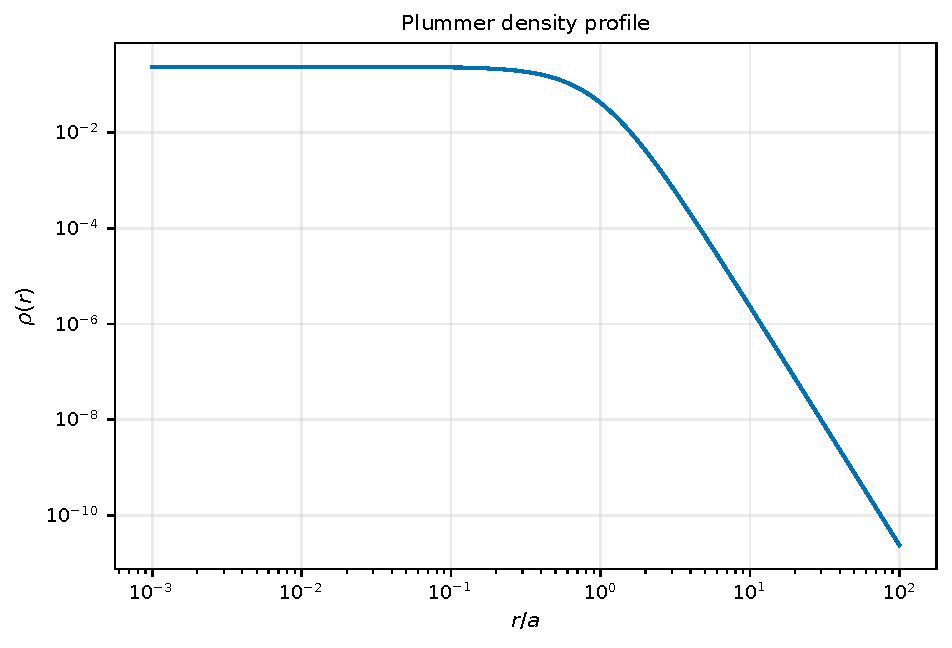
\includegraphics[width=\linewidth]{ch01_plummer_density.pdf}
\end{minipage}\hfill
\begin{minipage}[t]{0.47\linewidth}
\centering
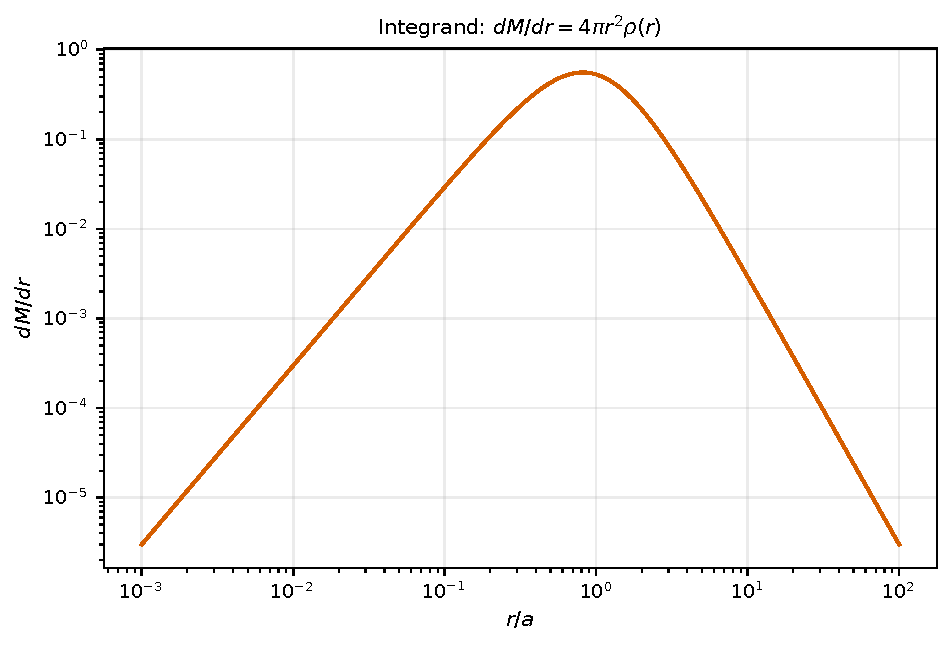
\includegraphics[width=\linewidth]{ch01_mass_integrand.pdf}
\end{minipage}
\caption{Plummer 密度分布の密度（左）と、内包質量の被積分関数 $dM/dr=4\pi r^2\rho$（右）。縦軸はそれぞれ $M/a^3$、$M/a$ を単位としている。密度は中心で最大であるが、同じ厚さの球殻の体積は $r^2$ に比例するため、$dM/dr$ は中心で0になる。}
\label{fig:ch1-plummer-integrand}
\end{figure}

\subsection{解析的な内包質量}

式\eqref{eq:ch1-plummer-density}のPlummer 密度分布では式\eqref{eq:ch1-enclosed-mass}を解析的に積分できる。
無次元半径
\begin{equation}
 x\equiv \frac{r}{a}
\label{eq:ch1-x-def}
\end{equation}
を導入する。積分変数を $u=r'/a$ に取り替えると、$r'=au$、$dr'=a\,du$ であり、積分の上端は $u=x$ になるので、
\begin{align}
 M(<r) =4\pi\int_0^r \rho(r')r'^2\,dr' =3M\int_0^x \frac{u^2}{(1+u^2)^{5/2}}\,du.
\label{eq:ch1-plummer-mass-int}
\end{align}
実際、
\begin{equation}
 \frac{d}{du}\left[\frac{u^3}{(1+u^2)^{3/2}}\right]
 =\frac{3u^2}{(1+u^2)^{5/2}}
\end{equation}
なので、この積分は解析的に計算できる。したがって、
\begin{equation}
 \boxed{
 M(<r)
 =M\frac{x^3}{(1+x^2)^{3/2}}
 =M\frac{(r/a)^3}{\left[1+(r/a)^2\right]^{3/2}}
 }
\label{eq:ch1-plummer-mass-exact}
\end{equation}
を得る。
$r\rightarrow\infty$ では $M(<r)\rightarrow M$ となり、$M$ が全質量であることも確認できる。
本章では式\eqref{eq:ch1-plummer-mass-exact}を「正解」として使い、数値積分の精度を検証する。

以後、本章では半径を $a$、質量を $M$ で規格化し、$r/a$ と $M(<r)/M$ を用いて結果を表す。
Notebook 1 では、この規格化を $M=a=1$ として実装する。
これは質量と長さの単位を選んで無次元量を扱っているだけであり、両者を同じ物理量とみなすことを意味しない。

\section{数値積分の考え方}
\label{sec:ch1-quadrature-basics}

数値積分の積分公式を導くため、ここでは $x$ を無次元半径に限らず一般の積分変数として用い、定積分
\begin{equation}
 I=\int_{x_0}^{x_N} f(x)\,dx
\label{eq:ch1-general-integral}
\end{equation}
を考える。
区間 $[x_0,x_N]$ を $N$ 個の小区間に等分し、格子点を
\begin{equation}
 x_i=x_0+ih,
 \qquad
 h=\frac{x_N-x_0}{N}
\label{eq:ch1-uniform-grid}
\end{equation}
とする。ここで $h$ は隣り合う格子点の間隔であり、\textbf{格子幅（grid spacing）}と呼ぶ。
$N$ は区間数であり、両端を含む格子点数は $N+1$ である。
この分割によって定積分$I$は
\begin{equation}
 I=\sum_{i=0}^{N-1}
 \int_{x_i}^{x_{i+1}} f(x)\,dx
\label{eq:ch1-split-integral}
\end{equation}
と書けることになる。

数値積分では、各小区間で $f(x)$ を簡単な関数で近似して積分する。
例えば一定値で近似すれば長方形、1次関数なら台形、2次関数なら Simpson 則が得られる。

\section{基本的な数値積分公式}
\label{sec:ch1-basic-rules}

図\ref{fig:ch1-quadrature-geometry}に、4種類の積分公式の幾何学的な考え方を示す\footnote{
ここでは4つの積分公式を紹介するが、格子点上の値を積分する実際の計算では台形則がよく使われる。
左長方形則は台形則と同じ格子点の値を使うにもかかわらず、誤差の減り方が遅い（\S\ref{sec:ch1-convergence}）。
中点則は区間の中点での値を必要とするため、格子点の値しかないデータにはそのまま使えない。
ただし、セル中心に値を置く計算や、端点で被積分関数が発散する積分では中点則が適している。
台形則は隣り合う2点の値だけで計算でき、不等間隔の格子にも使え、
区間ごとの面積を順に足すだけで累積積分が得られる（\S\ref{sec:ch1-cumulative}）。
Simpson 則は被積分関数が滑らかなときに誤差が速く減少するが、区間を2つずつ組にする必要があり、
折れ曲がりや雑音を含むデータでは、その利点は小さくなる。
格子法の流体計算で用いる有限体積法では、密度などのセル平均値を未知数とする。
一次元の Cartesian 座標で、幅 $h$ のセルを中心のまわりに対称に取ると、滑らかな関数のセル平均とセル中心の値との差は $O(h^2)$ となる。
この関係は、中点則の誤差と同じように Taylor 展開から説明できる\cite{matsumoto}。}。
以下では、各公式が被積分関数をどのように近似するかと、その実装方法を順に見ていく。
それぞれの方法で誤差がどの速さで減少するかは、後の収束試験で数値的に調べる。

\begin{figure}[!htbp]
\centering
\begin{minipage}[t]{0.47\linewidth}
\centering
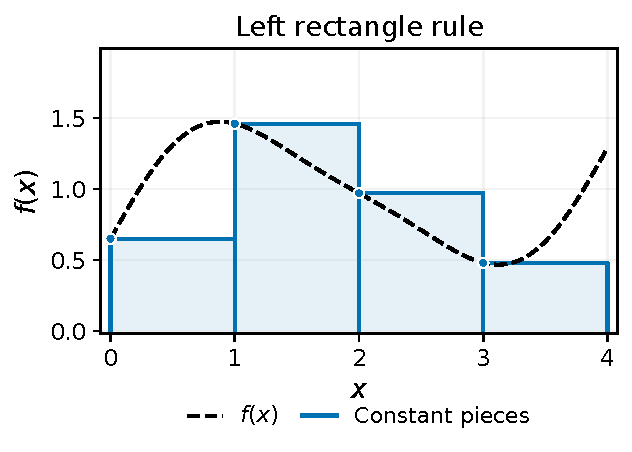
\includegraphics[width=\linewidth]{ch01_left_rule.pdf}\\[-1mm]
{\small (a) Left rectangle}
\end{minipage}\hfill
\begin{minipage}[t]{0.47\linewidth}
\centering
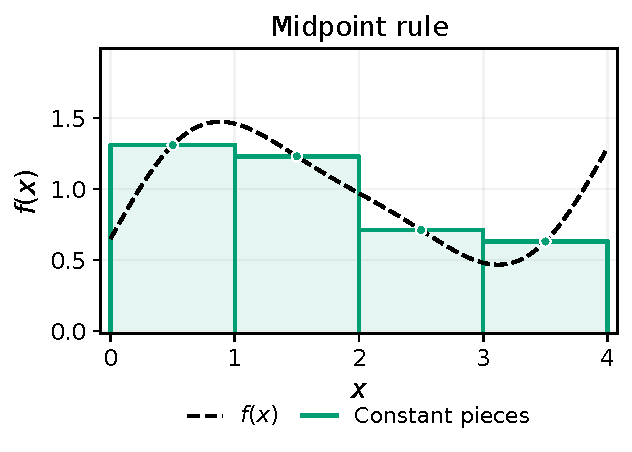
\includegraphics[width=\linewidth]{ch01_midpoint_rule.pdf}\\[-1mm]
{\small (b) Midpoint}
\end{minipage}

\vspace{2mm}
\begin{minipage}[t]{0.47\linewidth}
\centering
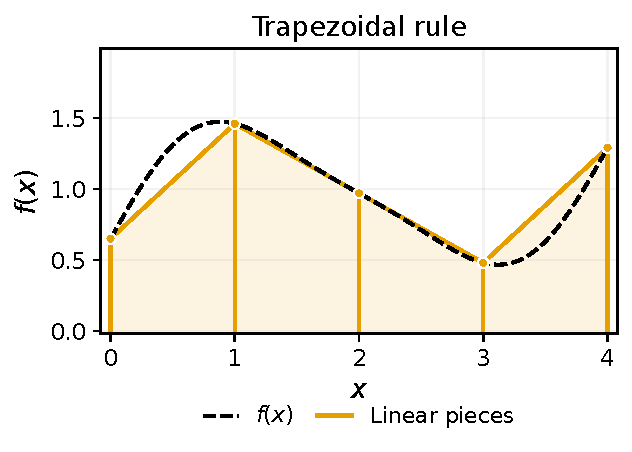
\includegraphics[width=\linewidth]{ch01_trapezoid_rule.pdf}\\[-1mm]
{\small (c) Trapezoidal}
\end{minipage}\hfill
\begin{minipage}[t]{0.47\linewidth}
\centering
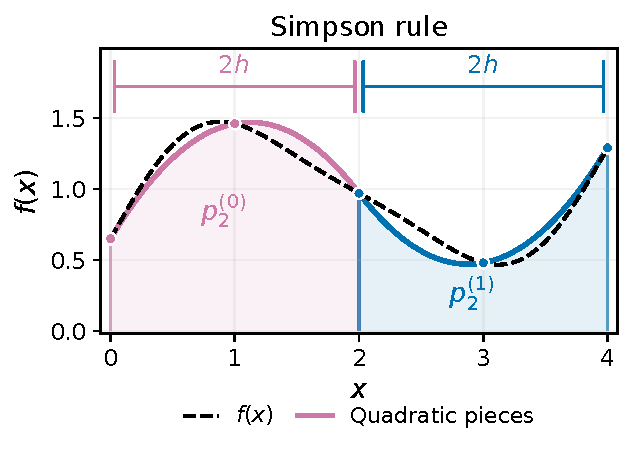
\includegraphics[width=\linewidth]{ch01_simpson_rule.pdf}\\[-1mm]
{\small (d) Simpson}
\end{minipage}
\caption{数値積分公式の幾何学的な意味。黒破線は全パネルで共通の被積分関数 $f(x)$、色付き実線は各方法の近似である。Simpson 則では幅 $2h$ の各区間で、3個の評価点を通る別々の二次多項式 $p_2^{(0)},p_2^{(1)}$ を積分する。色付きの面積が積分の近似値に対応する。}
\label{fig:ch1-quadrature-geometry}
\end{figure}

\subsection{左長方形則（left-rectangle rule）}

小区間 $[x_i,x_{i+1}]$ で $f(x)$ を左端の値 $f_i\equiv f(x_i)$ で一定と近似すると、
\begin{equation}
 \int_{x_i}^{x_{i+1}}f(x)\,dx
 \simeq hf_i
\label{eq:ch1-left-local}
\end{equation}
である。この近似では、各小区間の左端 $x_i=x_0+ih$ だけで関数を評価していることになる。
全区間を足すと、左長方形則は次のように書ける。
\begin{equation}
 \boxed{
 I_{\rm left}
 =h\sum_{i=0}^{N-1}f_i
 }
\label{eq:ch1-left-rule}
\end{equation}
Python では Listing 1.1 のように書ける。
\begin{listingbox}{1.1　左長方形則}
\begin{Verbatim}[fontsize=\small]
import numpy as np
def left_rule(func, x0, xN, N):
    h = (xN - x0) / N
    x = x0 + np.arange(N) * h
    return h * np.sum(func(x))
\end{Verbatim}
\end{listingbox}



\subsection{中点則（midpoint rule）}

小区間 $[x_i,x_{i+1}]$ で $f(x)$ を中点
\begin{equation}
 x_{i+1/2}=x_i+\frac{h}{2}
\label{eq:ch1-midpoint-def}
\end{equation}
での関数値を使えば、
\begin{equation}
 \boxed{
 I_{\rm mid}
 =h\sum_{i=0}^{N-1}f(x_{i+1/2})
 }
\label{eq:ch1-midpoint-rule}
\end{equation}
を得る。

中点 $x_{i+1/2}=x_i+h/2$ は、格子番号 $i$ に $1/2$ を加えて作れる。
式\eqref{eq:ch1-midpoint-rule}の実装が Listing 1.2 である。
\begin{listingbox}{1.2　中点則}
\begin{Verbatim}[fontsize=\small]
def midpoint_rule(func, x0, xN, N):
    h = (xN - x0) / N
    x_mid = x0 + (np.arange(N) + 0.5) * h
    return h * np.sum(func(x_mid))
\end{Verbatim}
\end{listingbox}


\subsection{台形則（trapezoidal rule）}

台形則では、小区間内の $f(x)$ を両端 $(x_i,f_i)$ と $(x_{i+1},f_{i+1})$ を結ぶ直線で近似する。
直線補間（linear interpolation）は
\begin{equation}
 f(x)
 \simeq f_i
 +\frac{f_{i+1}-f_i}{h}(x-x_i)
\label{eq:ch1-linear-interpolation}
\end{equation}
である。
これを $x_i$ から $x_{i+1}$ まで積分すると、
\begin{align}
 \int_{x_i}^{x_{i+1}}f(x)\,dx
 &\simeq
 \int_{x_i}^{x_{i+1}}
 \left[
 f_i+\frac{f_{i+1}-f_i}{h}(x-x_i)
 \right]dx \\
 &=\frac{h}{2}(f_i+f_{i+1}).
\label{eq:ch1-trapezoid-panel}
\end{align}
これが台形の面積そのものである。
全区間を足すと内部格子点は2回ずつ現れるため、
\begin{equation}
 \boxed{
 I_{\rm trap}
 =h\left[
 \frac{1}{2}f_0
 +\sum_{i=1}^{N-1}f_i
 +\frac{1}{2}f_N
 \right]
 }
\label{eq:ch1-trapezoid-rule}
\end{equation}
を得る。

式\eqref{eq:ch1-trapezoid-rule}の各項をそのまま Python に対応させると、Listing 1.3 のように書ける。
\begin{listingbox}{1.3　台形則}
\begin{Verbatim}[fontsize=\small]
def trapezoid_rule(func, x0, xN, N):
    h = (xN - x0) / N
    x = np.linspace(x0, xN, N + 1)
    y = func(x)

    return h * (0.5 * y[0] + np.sum(y[1:-1]) + 0.5 * y[-1])
\end{Verbatim}
\end{listingbox}
左長方形則と中点則では各小区間の代表点 $N$ 個を使ったが、台形則では両端を含む $N+1$ 個の格子点を使う。この実装では、それらを \texttt{np.linspace(x0, xN, N + 1)} で作っている。
$f_0$ と $f_N$ が \texttt{y[0]}, \texttt{y[-1]} に、
内部点の和 $\sum_{i=1}^{N-1}f_i$ が \texttt{np.sum(y[1:-1])} に対応する。


\subsection{Simpson 則（Simpson's rule）}
Simpson 則では、隣り合う2つの小区間を1組として扱う。まず1組 $[x_i,x_{i+2}]$ を取り出し、等間隔の3点
\begin{equation}
 x_i,\qquad x_{i+1}=x_i+h,\qquad x_{i+2}=x_i+2h
\label{eq:ch1-simpson-nodes}
\end{equation}
における関数値を $f_i,f_{i+1},f_{i+2}$ とする。
この3点を通る2次多項式で $f(x)$ を近似し、その多項式を積分する。

計算を簡単にするため、区間の中央 $x_{i+1}$ を原点とする無次元変数
\begin{equation}
 t=\frac{x-x_{i+1}}{h}
\label{eq:ch1-simpson-t}
\end{equation}
を導入する。このとき、3点は $t=-1,0,1$ に対応する。
2次多項式を
\begin{equation}
 p_2(t)=At^2+Bt+C
\end{equation}
とおく。3点を通る条件は
\begin{align}
 p_2(-1)&=A-B+C=f_i,\\
 p_2(0)&=C=f_{i+1},\\
 p_2(1)&=A+B+C=f_{i+2}
\end{align}
である。これらを解くと、
\begin{equation}
 A=\frac{f_i-2f_{i+1}+f_{i+2}}{2},\qquad
 B=\frac{f_{i+2}-f_i}{2},\qquad
 C=f_{i+1}
\end{equation}
を得る。

$dx=h\,dt$ なので、
\begin{align}
 \int_{x_i}^{x_{i+2}}f(x)\,dx
 &\simeq h\int_{-1}^{1}p_2(t)\,dt
 \label{eq:ch1-simpson-integral-p2}\\
 &=h\int_{-1}^{1}(At^2+Bt+C)\,dt \notag\\
 &=h\left(\frac{2A}{3}+2C\right) \notag\\
 &=\frac{h}{3}(f_i+4f_{i+1}+f_{i+2})
 \label{eq:ch1-simpson-panel}
\end{align}
を得る。
これが1組に対する Simpson の1/3公式である\cite{kouya2021}。

次に、積分区間全体を幅 $h$ の $N$ 個の小区間に分割する。
Simpson 則は2つの小区間を1組として適用するため、$N$ は偶数とする。
例えば、$N=4$ の場合を考える。
最初の組 $[x_0,x_2]$ と次の組 $[x_2,x_4]$ にSimpson 則を適用して足し合わせると、
\begin{align}
 I_{\rm Simpson}
 &=
 \frac{h}{3}(f_0+4f_1+f_2)
 +\frac{h}{3}(f_2+4f_3+f_4)\\
 &=
 \frac{h}{3}(f_0+4f_1+2f_2+4f_3+f_4)
\end{align}
となる。
ここで、$f_2$ は両方の組に含まれるため、係数が2になる。
同様に、$N$ が一般の偶数の場合には、積分区間の両端の係数が1、奇数番号の点の係数が4、
両端を除く偶数番号の点の係数が2となる。したがって、
\begin{equation}
 \boxed{
 I_{\rm Simpson}
 =\frac{h}{3}\left[
 f_0+f_N
 +4\sum_{j=1}^{N/2}f_{2j-1}
 +2\sum_{j=1}^{N/2-1}f_{2j}
 \right]
 }
\label{eq:ch1-composite-simpson}
\end{equation}
を得る。

この公式では、奇数番号と偶数番号の内部点を別々に足す必要がある。
NumPy のスライスを使うと、Listing 1.4 のように数式の構造をほぼそのまま表現できる。
\begin{listingbox}{1.4　Simpson 則}
\begin{Verbatim}[fontsize=\small]
def simpson_rule(func, x0, xN, N):
    if N % 2 != 0:
        raise ValueError("Simpson 則では N を偶数にしてください。")

    h = (xN - x0) / N
    x = np.linspace(x0, xN, N + 1)
    y = func(x)

    odd_sum = np.sum(y[1:-1:2])
    even_sum = np.sum(y[2:-1:2])

    return h / 3.0 * (y[0] + y[-1] + 4.0 * odd_sum + 2.0 * even_sum)
\end{Verbatim}
\end{listingbox}

\texttt{y[1:-1:2]} は $y_1,y_3,y_5,\ldots$、
\texttt{y[2:-1:2]} は $y_2,y_4,y_6,\ldots$ を取り出す。
したがって、それぞれ式\eqref{eq:ch1-composite-simpson}の奇数番号の和と偶数番号の和に対応する。


\section{Plummer 球による4つの積分法の比較}
\label{sec:ch1-compare-rules}

Plummer 球について、半径 $r=a$ までの内包質量を求める。$x=r/a$ を用いると、
式\eqref{eq:ch1-plummer-mass-int}より、比較する積分は
\begin{equation}
 I\equiv\frac{M(<a)}{M}=\int_0^1\frac{3x^2}{(1+x^2)^{5/2}}\,dx
\label{eq:ch1-plummer-test-integral}
\end{equation}
である。すなわち、$f(x)=3x^2/(1+x^2)^{5/2}$ に前節で導いた4つの積分公式を適用する。
この $f(x)$ は、式\eqref{eq:ch1-mass-integrand}の被積分関数 $f_M(r)=dM/dr$ を $M/a$ で割り、$r=ax$ としたものである。Notebook 1 では $M=a=1$ とするため、\texttt{dMdr\_plummer} の返す値がそのまま $f(x)$ に対応する。

数値積分の精度を評価するために、格子幅 $h$ で求めた数値積分値を $I_h$ とし、解析値 $I$ との差の大きさ
\begin{equation}
 \epsilon(h)\equiv |I_h-I|
\label{eq:ch1-absolute-error}
\end{equation}
を\textbf{絶対誤差（absolute error）}と定義する。これは、全質量 $M$ で規格化した内包質量の誤差である。
なお、ここでは $r=a$ を評価点とし、解析値
\begin{equation}
 I=\frac{M(<a)}{M}=\frac{1}{2\sqrt{2}}
 \simeq \choneMExactA
\label{eq:ch1-mass-at-a}
\end{equation}
を比較基準とする。

\begin{notebookblock}{1｜4つの積分法の比較}
$M=a=1$、$N=40$ として、4つの積分法を同じ条件で比較する。数値積分値と解析値との差から絶対誤差を計算し、その結果を同じセルの出力として表示する。

{\sffamily\small\color{graytext}対応セル（計算部分）}
\begin{Verbatim}[xleftmargin=2mm,fontsize=\small,frame=single,framesep=1.8mm,framerule=0.35pt,rulecolor=\color{listingframe},fillcolor=\color{listingbg}]
# 積分区間を 0 <= r <= a とし、区間数を N=40 にする
r_eval = 1.0 * a
N = 40

# 被積分関数 dM/dr = 4 pi r^2 rho(r)
func = lambda r: dMdr_plummer(r, M, a)

# 同じ条件で4つの数値積分法を適用する
m_left = left_rule(func, 0.0, r_eval, N)
m_mid = midpoint_rule(func, 0.0, r_eval, N)
m_trap = trapezoid_rule(func, 0.0, r_eval, N)
m_simp = simpson_rule(func, 0.0, r_eval, N)

# 数値積分値と比較する解析値
m_exact_eval = mass_plummer_exact(r_eval, M, a)

print(f"解析値     : {m_exact_eval:.12f}")
print(f"左長方形則  : {m_left:.12f}   誤差 = {abs(m_left - m_exact_eval):.3e}")
print(f"中点則     : {m_mid:.12f}   誤差 = {abs(m_mid - m_exact_eval):.3e}")
print(f"台形則     : {m_trap:.12f}   誤差 = {abs(m_trap - m_exact_eval):.3e}")
print(f"Simpson 則 : {m_simp:.12f}   誤差 = {abs(m_simp - m_exact_eval):.3e}")
\end{Verbatim}

{\sffamily\small\color{graytext}実行結果}
\begin{Verbatim}[numbers=none,fontsize=\small]
解析値                : 0.353553390593
左長方形則            : 0.346910451143   誤差 = 6.643e-03
中点則                : 0.353560298293   誤差 = 6.908e-06
台形則                : 0.353539577216   誤差 = 1.381e-05
Simpson 則            : 0.353553401385   誤差 = 1.079e-08
\end{Verbatim}
\end{notebookblock}

この結果から、$N=40$ では Simpson 則の誤差が最も小さいことがわかる。
しかし、この1つの格子だけでは、格子を細かくしたときに誤差がどのように減るかは分からない。
そこで次に、格子幅と絶対誤差 $\epsilon(h)$の関係を調べる収束試験を行う。

\section{収束次数の測定}
\label{sec:ch1-convergence}

\subsection{誤差の $h$ 依存性}

前節では、$N=40$ の1つの格子で4つの積分法の誤差を比較した。
次に、格子幅 $h$ を小さくしたときに、絶対誤差 $\epsilon(h)$ がどの速さで減少するかを調べる。
多くの数値計算法では、格子を十分に細かくすると、誤差は格子幅 $h$ のべき乗に従って規則的に減少する。
この誤差の減少の速さを表す量を\textbf{収束次数}という。

\begin{definitionbox}{収束次数}
十分小さい格子幅 $h$ に対して、誤差が
\begin{equation}
 \epsilon(h)\simeq C h^p
\label{eq:ch1-error-model}
\end{equation}
と振る舞うとき、指数 $p>0$ をその数値計算法の\textbf{収束次数（order of convergence）}と呼ぶ。
ここで $C>0$ は $h$ に依存しない定数である。
\end{definitionbox}

収束次数が $p$ の方法を、\textbf{$p$ 次精度}の方法と呼ぶ。
例えば $p=2$ なら、格子幅を半分にすると誤差はおよそ $1/4$ になる。
$p=4$ なら、およそ $1/16$ になる。
したがって、収束次数が大きい方法ほど、格子を細かくしたときに誤差が速く減少する。

\begin{cautionblock}{収束次数と誤差の大きさは同じではない}
式\eqref{eq:ch1-error-model}では、収束次数 $p$ は格子幅を小さくしたときに誤差がどの速さで減るかを表し、係数 $C$ は誤差の大きさに関係する。
したがって、同じ収束次数をもつ方法でも、同じ $h$ での誤差が同じとは限らない。
また、有限の $h$ では、収束次数が高い方法が必ず最小の誤差を与えるとは限らない。
\end{cautionblock}

\subsection{数値実験による収束次数の測定}

それでは、Plummer 球の内包質量を用いて、実際に収束次数を測ってみる。
収束次数を数値的に測定するには、式\eqref{eq:ch1-error-model}の対数を取り、
\begin{equation}
 \log\epsilon
 =p\log h+\log C
\label{eq:ch1-log-error}
\end{equation}
とする。
したがって、$\log\epsilon$ を $\log h$ に対してプロットすると、式\eqref{eq:ch1-error-model}が成り立つ範囲では点列はほぼ直線上に並び、その傾きが収束次数 $p$ となる。
対数の底を変えても傾き $p$ は変わらない。Notebook 1 では、\texttt{np.log} と \texttt{np.polyfit} を用いて複数の格子幅の点を直線で近似し、その傾きから $p$ を求める。

そこで、複数の格子幅で同じ積分を計算し、解析値との差から得た絶対誤差を用いて収束次数を測定する。
どの積分公式で $p$ がどの程度になるかを、まず数値実験から確かめてみる。

\begin{notebookblock}{1｜収束試験}
左長方形則・中点則・台形則・Simpson 則について、$N=10,20,40,80,160,320$ と格子を細かくする。各方法について $\log\epsilon$ と $\log h$ を直線で近似し、その傾きから収束次数 $p$ を求める。
そのために、ここでは NumPy の \texttt{np.polyfit(x, y, 1)} を用いる。
この関数は、データ $(x,y)$ を直線 $y=ax+b$ で最小二乗近似し、傾き $a$ と切片 $b$ をこの順に返す。
したがって、末尾の \texttt{[0]} で傾き、すなわち収束次数 $p$ を取り出す。

{\sffamily\small\color{graytext}対応セル（計算部分）}
\begin{Verbatim}[xleftmargin=2mm,fontsize=\small,frame=single,framesep=1.8mm,framerule=0.35pt,rulecolor=\color{listingframe},fillcolor=\color{listingbg}]
# 区間数 N を2倍ずつ増やして格子幅を小さくする
N_values = np.array([10, 20, 40, 80, 160, 320])
h_values = r_eval / N_values

# 4つの積分法を同じ形で呼び出せるようにまとめる
methods = {
    "Left rectangle": lambda N: left_rule(func, 0.0, r_eval, N),
    "Midpoint": lambda N: midpoint_rule(func, 0.0, r_eval, N),
    "Trapezoidal": lambda N: trapezoid_rule(func, 0.0, r_eval, N),
    "Simpson": lambda N: simpson_rule(func, 0.0, r_eval, N),
}

errors = {}
orders = {}
for name, method in methods.items():
    # 各 N で解析値との差を絶対誤差として測る
    err = np.array([abs(method(int(N)) - m_exact_eval) for N in N_values])
    errors[name] = err

    # log(error)-log(h) の傾きから収束次数 p を求める
    orders[name] = np.polyfit(np.log(h_values), np.log(err), 1)[0]

method_names_ja = {
    "Left rectangle": "左長方形則",
    "Midpoint": "中点則",
    "Trapezoidal": "台形則",
    "Simpson": "Simpson 則",
}

for name in methods:
    print(f"{method_names_ja[name]:10s}: 測定した収束次数 = {orders[name]:.3f}")
\end{Verbatim}

{\sffamily\small\color{graytext}実行結果}
\begin{Verbatim}[numbers=none,fontsize=\small]
左長方形則     : 測定した収束次数 = 1.002
中点則         : 測定した収束次数 = 2.001
台形則         : 測定した収束次数 = 2.001
Simpson 則     : 測定した収束次数 = 4.001
\end{Verbatim}
\end{notebookblock}

この結果から、左長方形則はほぼ1次、中点則と台形則はほぼ2次、Simpson 則はほぼ4次で収束していることがわかる。
また、誤差と格子幅の関係を図\ref{fig:ch1-convergence}に示す。各方法の点列は両対数表示でほぼ直線となり、その傾きがそれぞれの収束次数に対応している。

このような\textbf{格子収束試験（grid-convergence test）}は、数値計算法の収束次数を実際の計算から調べる基本的な検証方法である。ただし、格子を極端に細かくすると、誤差がこのべき則から外れる場合がある。その主な原因の一つが、次節で扱う浮動小数点演算の丸め誤差である。

\begin{figure}[!htbp]
\centering
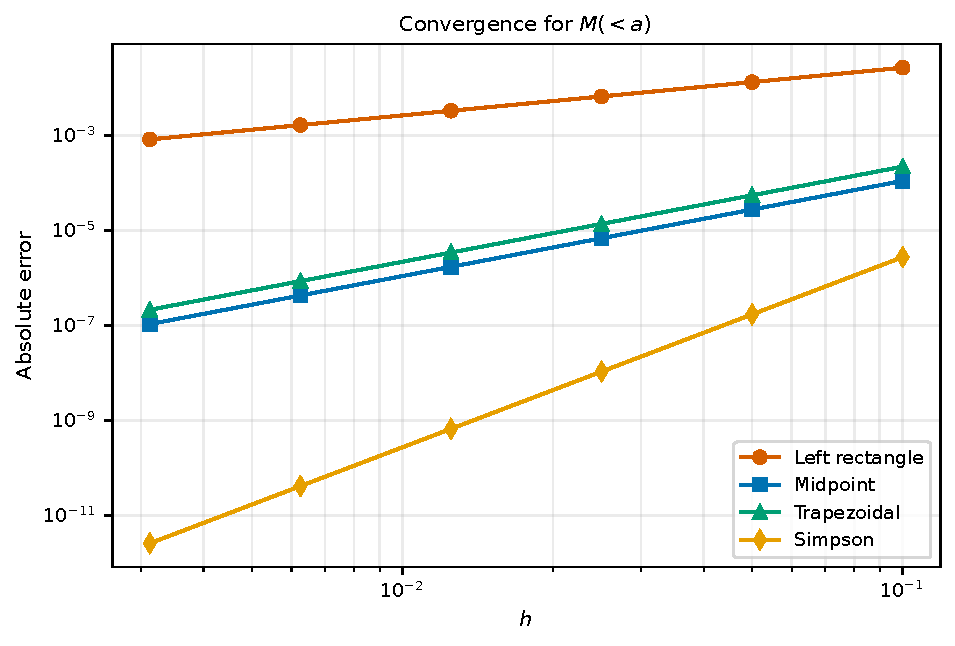
\includegraphics[width=0.6\linewidth]{ch01_convergence.pdf}
\caption{$M(<a)/M$ の絶対誤差と格子幅 $h$ の関係。両対数表示での傾きが収束次数 $p$ である。ここで $h$ は無次元半径 $x=r/a$ に対する格子幅であり、$h=1/N$ である。}
\label{fig:ch1-convergence}
\end{figure}



\begin{topicblock}{Taylor 展開から収束次数を理解する}
ここまでの収束試験では、数値実験から左長方形則、中点則、台形則、Simpson 則の収束次数を測定した。
ここでは中点則を例に、なぜ局所的な近似誤差から積分全体の収束次数が決まるのかを見る。
この補足は、以後の節を理解するための必須事項ではない。

以下で $O(h^q)$ は、$h\rightarrow0$ のとき、その項の大きさが $h^q$ の定数倍以下に抑えられることを表す。
1区間で生じる誤差を\textbf{局所打ち切り誤差}、積分区間全体で得られる誤差を\textbf{大域誤差}と呼ぶ。

中点則を区間 $[x_i,x_{i+1}]$ に適用する。
区間幅を $h=x_{i+1}-x_i$、中点を
\begin{equation}
 x_{i+1/2}=\frac{x_i+x_{i+1}}{2}
\end{equation}
とする。
中点からのずれを $\xi=x-x_{i+1/2}$ とおけば、積分範囲は
$-h/2\le\xi\le h/2$ となる。
中点のまわりで Taylor 展開すると、
\begin{equation}
 f(x_{i+1/2}+\xi)
 =
 f_{i+1/2}
 +\xi f'_{i+1/2}
 +\frac{\xi^2}{2}f''_{i+1/2}
 +\frac{\xi^3}{6}f'''_{i+1/2}
 +O(\xi^4)
\end{equation}
である。
これを $-h/2$ から $h/2$ まで積分する。
対称な区間では $\xi$ と $\xi^3$ のような奇数次の項の積分が0になるので、
\begin{align}
 \int_{x_i}^{x_{i+1}}f(x)\,dx
 &=
 \int_{-h/2}^{h/2}f(x_{i+1/2}+\xi)\,d\xi \notag\\
 &=
 h f_{i+1/2}
 +\frac{h^3}{24}f''_{i+1/2}
 +O(h^5)
\label{eq:ch1-midpoint-error-advanced}
\end{align}
を得る。

中点則は右辺の最初の項 $h f_{i+1/2}$ だけを使う。
したがって、1区間での局所打ち切り誤差は
\begin{equation}
 E_i
 =
 \frac{h^3}{24}f''_{i+1/2}
 +O(h^5)
 =
 O(h^3)
\end{equation}
である。

次に、積分区間全体 $[a,b]$ を考える。
区間数は
\begin{equation}
 N=\frac{b-a}{h}\propto h^{-1}
\end{equation}
である。
$f''$ が積分区間で有界なら、各区間の局所打ち切り誤差は一様に $O(h^3)$ なので、
それらを $N$ 区間にわたって合わせた大域誤差は
\begin{equation}
 E
 =\sum_{i=0}^{N-1}E_i
 =O(Nh^3)
 =O(h^2)
\end{equation}
となる。
したがって、中点則は\textbf{2次精度}である。

他の積分公式でも考え方は同じである。
局所打ち切り誤差が $O(h^{p+1})$ なら、固定した積分区間では区間数が
$O(h^{-1})$ であるため、大域誤差は $O(h^p)$ となる。本章で用いた4つの公式では以下のようになる。
なお、Simpson 則では2区間1組を単位として局所誤差を数えるが、
組の数も $O(h^{-1})$ なので同じ考え方で4次精度が得られる。
\begin{center}
\begin{tabular}{lcc}
\toprule
方法 & 局所打ち切り誤差 & 大域誤差 \\
\midrule
左長方形則 & $O(h^2)$ & $O(h)$ \\
中点則 & $O(h^3)$ & $O(h^2)$ \\
台形則 & $O(h^3)$ & $O(h^2)$ \\
Simpson 則 & $O(h^5)$ & $O(h^4)$ \\
\bottomrule
\end{tabular}
\end{center}

この結果は、Notebook 1 の収束試験で測定した
$p\simeq1,2,2,4$ と一致する。
より一般的な積分則の誤差評価については杉浦 第3章\cite{sugiura2009}を、
Newton--Cotes 型積分公式の導出と実装については幸谷 第12章\cite{kouya2021}を参照されたい。
\end{topicblock}

\section{離散化誤差と丸め誤差}
\label{sec:ch1-roundoff}

前節の収束試験では、格子幅 $h$ を小さくすると、数値積分の誤差が $h^p$ に従って減少することを確認した。
数値計算では、このような数値公式による近似だけでなく、計算機が有限桁の数を扱うことによっても誤差が生じる。
本節では、これらに対応する\textbf{離散化誤差}と\textbf{丸め誤差}について考える。

\subsection{離散化誤差（discretization error）}

数値計算では、連続な問題をそのまま計算機で扱うのではなく、有限個の格子点や時間刻みを用いた離散的な問題に置き換える。
本章の数値積分では、積分区間を有限個の小区間に分け、それぞれの区間で被積分関数を簡単な関数で近似した。
このような離散化によって、数値積分値には厳密な積分値との差が生じる。
この差を\textbf{離散化誤差（discretization error）}という。

離散化によって生じる誤差は、「1回の近似でどれだけずれるか」と「計算全体の結果がどれだけずれるか」という2つの観点から見ることができる。
数値積分では、各小区間で近似を行うたびに誤差が生じ、それらを全区間に適用した最終的な積分値にも誤差が残る。
この2つの見方に対応するのが、局所打ち切り誤差と大域誤差である。

\begin{definitionbox}{局所打ち切り誤差と大域誤差}
微分、積分、時間発展などの連続な関係を有限の近似式へ置き換えたときに生じるずれを
\textbf{打ち切り誤差（truncation error）}という。
本書では、1つの小区間、1ステップ、または1格子点で評価したものを
\textbf{局所打ち切り誤差（local truncation error）}と呼ぶ。

一方、離散公式を計算全体に適用して得られた数値結果と厳密な結果との差を
\textbf{大域誤差（global error）}という。
本章の数値積分では、丸め誤差などを無視できる場合、大域誤差は各区間の局所的な打ち切り誤差を積分範囲全体で合わせた結果として現れる。
時間発展を伴う問題では、局所的な誤差の伝播や増幅も重要になる。
\end{definitionbox}

前節の収束試験で測定した収束次数 $p$ は、この大域誤差が格子幅 $h$ に対してどの速さで減少するかを表している。
本章の例では、左長方形則の誤差はおよそ $h$、中点則と台形則では $h^2$、Simpson 則では $h^4$ に比例して減少した。
離散化誤差だけを考えるなら、格子幅 $h$ を小さくするほど数値積分値は解析値に近づく。

\subsection{丸め誤差（round-off error）}

実際の計算機では、実数を無限の精度で表すことはできない。
数値計算では、実数を有限桁の\textbf{浮動小数点数（floating-point number）}で近似して扱う。
浮動小数点数とは、例えば $1.23\times 10^4$ のように、数を有効数字と指数に分けて表す方法である。
計算機では通常、2進数を用いて数を表すが、表現できる有効桁数には限りがある。
そのため、演算結果が表現可能な数に一致しない場合には、近くの値へ丸められる。
このように、有限桁の浮動小数点数で数値を表し、演算結果を丸めることによって生じる誤差を
\textbf{丸め誤差（round-off error）}という。

浮動小数点数の精度を表す目安の一つが、\textbf{機械イプシロン（machine epsilon）}である。
機械イプシロン $\epsilon_{\rm mach}$ は、1と、それより大きい最も近い浮動小数点数との差として定義される。
つまり、1付近でどれほど小さな数の差を区別できるかを表している。
Notebook 1 で用いる倍精度浮動小数点数（64ビット）では、
\begin{equation}
 \epsilon_{\rm mach}\simeq \choneMachineEps
\label{eq:ch1-machine-eps}
\end{equation}
である\cite{kouya2021}。
ただし、機械イプシロンは計算結果全体の誤差を表すものではない。
丸め誤差は演算を繰り返すことで蓄積する場合がある。
また、近い値どうしを引くと、もとの数値に含まれる小さな誤差が計算結果に大きく影響することがある。

一般に、格子を細かくすると離散化誤差は小さくなる。
しかし、離散化誤差が十分に小さくなると、丸め誤差の影響を無視できなくなる場合がある。
そのため、格子を細かくしても計算精度が上がり続けるとは限らない。
Simpson 則では離散化誤差がおよそ $h^4$ に比例して速く減少するため、この変化を確認しやすい。

\begin{notebookblock}{1｜Simpson 則と丸め誤差}
$N\sim10^3$--$10^4$ 以上まで増やし、離散化誤差が十分小さくなった後に丸め誤差の影響が現れる様子を確認する。

{\sffamily\small\color{graytext}対応セル（計算部分）}
\begin{Verbatim}[xleftmargin=2mm,fontsize=\small,frame=single,framesep=1.8mm,framerule=0.35pt,rulecolor=\color{listingframe},fillcolor=\color{listingbg}]
# Simpson 則で、さらに細かい格子まで調べる
N_large = np.array([320, 640, 1280, 2560,
                    5120, 10240, 20480])
err_large = []

for N_i in N_large:
    # 各 N で Simpson 則を適用し、解析値との誤差を保存する
    val = simpson_rule(func, 0.0, r_eval, int(N_i))
    err_large.append(abs(val - m_exact_eval))

# 倍精度浮動小数点数の機械イプシロン
machine_eps = np.finfo(float).eps
\end{Verbatim}
\end{notebookblock}

図\ref{fig:ch1-roundoff}に示すように、この計算では区間数を増やすと、
最初は $h^4$ に従って誤差が減少する。
しかし、誤差が $10^{-15}$--$10^{-16}$ 程度まで小さくなると
丸め誤差の影響が現れ、この関係から外れる。
この領域では、格子をさらに細かくしても精度は系統的には向上しない。

\begin{figure}[!htbp]
\centering
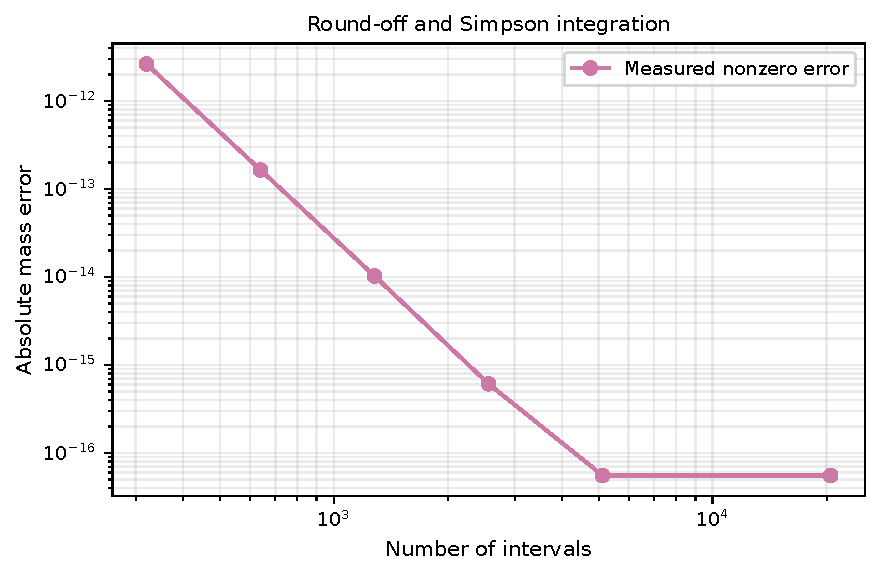
\includegraphics[width=0.68\linewidth]{ch01_roundoff.pdf}
\caption{Simpson 則の区間数 $N$ を増やしたときの、$M(<a)/M$ の絶対誤差。
離散化誤差が十分小さくなると、倍精度浮動小数点数の丸め誤差の影響が見えてくる。}
\label{fig:ch1-roundoff}
\end{figure}


\section{累積積分による内包質量プロファイル}
\label{sec:ch1-cumulative}

これまでは固定した半径 $r=a$ までの1つの定積分を比較した。次に、すべての格子点 $r_i$ について $M(<r_i)$ を求める。
しかし、各半径について0から積分をやり直すと、同じ区間の寄与を何度も計算することになる。
隣の区間の寄与を順に加える\textbf{累積積分（cumulative integration）}を使えば、この重複を避けられる。
台形則では、隣り合う2点の値から各区間の積分を求められるため、寄与を順に足し上げやすい。また、区間幅が一定でない格子にも同じ形で適用できる。

中心 $r_0=0$ から外側へ並ぶ格子 $r_0<r_1<\cdots<r_N$ を考え、$M(<r_i)$ の数値近似を $M_i$ と書く。
格子は不等間隔でもよいように、
\begin{equation}
 \Delta r_i=r_{i+1}-r_i
\label{eq:ch1-nonuniform-dr}
\end{equation}
とする。
被積分関数を
\begin{equation}
 f_{M,i}=4\pi r_i^2\rho(r_i)
\label{eq:ch1-gi}
\end{equation}
とすると、台形則で各区間の質量は
\begin{equation}
 \Delta M_i
 \simeq
 \frac{f_{M,i}+f_{M,i+1}}{2}\Delta r_i
\label{eq:ch1-delta-mi}
\end{equation}
である。
したがって
\begin{equation}
 M_{i+1}=M_i+\Delta M_i,
 \qquad M_0=0
\label{eq:ch1-cumulative-recurrence}
\end{equation}
として中心から外側へ順に加えれば、全格子点の内包質量を得られる。

この手順を NumPy の配列演算で書くと、隣り合う2点の台形面積を一度に計算し、
\texttt{np.cumsum} で左から累積できる。

\begin{listingbox}{1.5　累積台形積分}
\begin{Verbatim}[fontsize=\small]
def cumulative_trapezoid_manual(x, y):
    result = np.zeros_like(x, dtype=float)

    dx = np.diff(x)
    area = 0.5 * (y[:-1] + y[1:]) * dx

    result[1:] = np.cumsum(area)
    return result
\end{Verbatim}
\end{listingbox}

\begin{notebookblock}{1｜内包質量プロファイル}
$r_{\max}=20a$ まで400格子点を置き、Listing 1.5 の累積台形積分を使って $M(<r)$ を求める。

{\sffamily\small\color{graytext}対応セル（計算部分）}
\begin{Verbatim}[xleftmargin=2mm,fontsize=\small,frame=single,framesep=1.8mm,framerule=0.35pt,rulecolor=\color{listingframe},fillcolor=\color{listingbg}]
# 0 <= r <= 20a に400個の格子点を置く
N_profile = 400
r_max = 20.0 * a
r = np.linspace(0.0, r_max, N_profile)

# 各格子点で被積分関数 dM/dr を評価する
dMdr = dMdr_plummer(r, M, a)

# 累積台形則で M(<r) を外側へ順に積み上げる
m_num = cumulative_trapezoid_manual(r, dMdr)

# 同じ格子点で解析解も計算して比較する
m_exact = mass_plummer_exact(r, M, a)
\end{Verbatim}
\end{notebookblock}

ここで \texttt{np.linspace} は、指定した範囲の両端を含む格子点を等間隔に配置する。
ここでは400個の格子点を置くため、隣り合う格子点の間の区間数は399となる。
図\ref{fig:ch1-enclosed-mass}に示すように、得られた数値積分の結果は解析式とほぼ重なる。

\begin{figure}[!htbp]
\centering
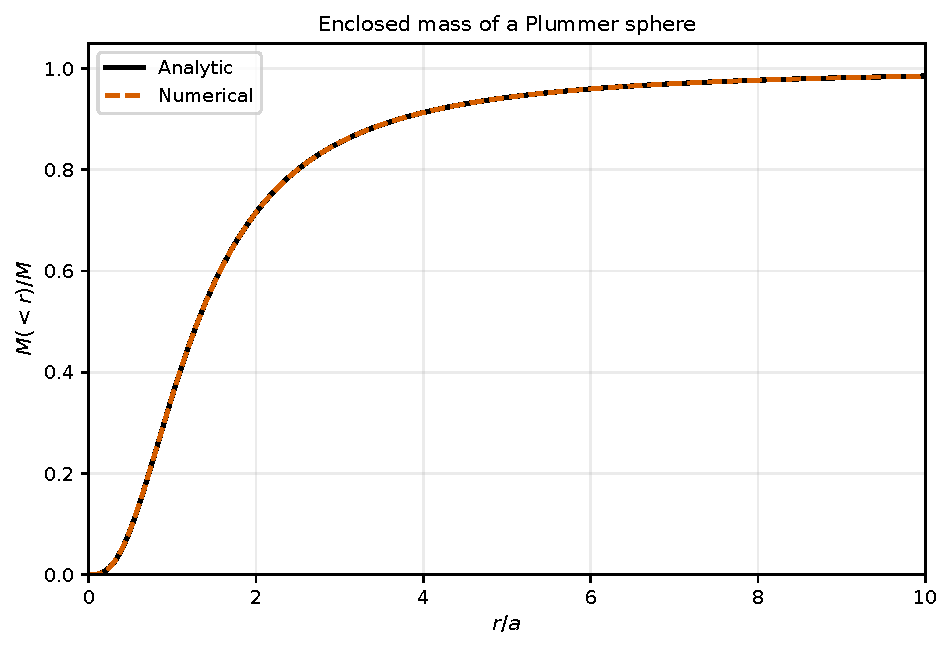
\includegraphics[width=0.68\linewidth]{ch01_enclosed_mass.pdf}
\caption{Plummer 球の内包質量。台形則による累積数値積分と解析解を比較している。計算は $r_{\max}=20a$ まで行い、図は $r\le10a$ の範囲を示す。}
\label{fig:ch1-enclosed-mass}
\end{figure}


\section{内包質量と円運動速度}
\label{sec:ch1-circular-speed}

球対称系では Newton の球殻定理（shell theorem）により、半径 $r$ における重力加速度は、その半径より内側の質量 $M(<r)$ だけで決まる。
ここで $G$ は万有引力定数、$g_r$ は重力加速度の動径成分とし、動径方向は外向きを正に取る。
このとき
\begin{equation}
 g_r(r)=-\frac{GM(<r)}{r^2}
\label{eq:ch1-spherical-gravity}
\end{equation}
である。

半径 $r$ の円軌道を速さ $v_{\rm circ}$ で運動する粒子の半径方向加速度は
\begin{equation}
 a_r=-\frac{v_{\rm circ}^2}{r}
\end{equation}
である。
円運動では、この加速度を重力が与えるので $a_r=g_r$ である。したがって、
\begin{equation}
 -\frac{v_{\rm circ}^2}{r}
 =-\frac{GM(<r)}{r^2}
\end{equation}
となり、
\begin{equation}
 \boxed{
 v_{\rm circ}(r)
 =\sqrt{\frac{GM(<r)}{r}}
 }
\label{eq:ch1-circular-speed}
\end{equation}
を得る\cite{ryden2025}。
式\eqref{eq:ch1-circular-speed}は $r>0$ について書いた式である。
Plummer 球では中心付近で $M(<r)\simeq M(r/a)^3$ なので、$v_{\rm circ}\simeq \sqrt{GM/a^3}\,r$ となり、$r\rightarrow0$ で $v_{\rm circ}\rightarrow0$ である。
Notebook 1 では、この極限に対応して $r=0$ の値を0として扱う。
円運動速度を半径の関数として表したものを\textbf{回転曲線（rotation curve）}と呼ぶ。
したがって、数値積分によって $M(<r)$ が得られれば、式\eqref{eq:ch1-circular-speed}から回転曲線を計算できる。

Plummer 球では内包質量の解析式も分かっているため、回転曲線を解析的に求めることもできる。
式\eqref{eq:ch1-plummer-mass-exact}を式\eqref{eq:ch1-circular-speed}に代入すると、
\begin{equation}
 v_{\rm circ}^2(r)
 =\frac{GMr^2}{(r^2+a^2)^{3/2}}
\label{eq:ch1-plummer-vc}
\end{equation}
となる。
この解析式は、数値積分で得た $M(<r)$ から計算した回転曲線を検証する基準として使える。

ここで、速度の単位を
\begin{equation}
 v_\ast\equiv\sqrt{\frac{GM}{a}}
\label{eq:ch1-velocity-unit}
\end{equation}
とし、無次元半径 $x=r/a$ を導入する。
式\eqref{eq:ch1-plummer-vc}は
\begin{equation}
 \frac{v_{\rm circ}^2}{v_\ast^2}
 =\frac{x^2}{(1+x^2)^{3/2}}
\label{eq:ch1-plummer-vc2}
\end{equation}
となる。
Notebook 1 では $G=M=a=1$ としているため、$v_\ast=1$ である。
物理単位へ戻すには、得られた無次元速度に $v_\ast=\sqrt{GM/a}$ を掛ければよい。

この解析式を使えば、回転曲線が最大となる半径も求められる。
$v_{\rm circ}>0$ なので、$v_{\rm circ}$ を最大にする半径は $v_{\rm circ}^2$ を最大にする半径と同じである。
式\eqref{eq:ch1-plummer-vc2}の右辺を
\begin{equation}
 q(x)=x^2(1+x^2)^{-3/2}
\label{eq:ch1-qx}
\end{equation}
と置く。
微分すると
\begin{equation}
 \frac{dq}{dx}
 =\frac{x(2-x^2)}{(1+x^2)^{5/2}}.
\label{eq:ch1-q-prime}
\end{equation}
$x>0$ で $dq/dx=0$ を満たすのは $x=\sqrt{2}$ である。
導関数はこの点の前後で正から負に変わるため、円運動速度が最大となる半径は
\begin{equation}
 r_{\rm peak}=\sqrt{2}\,a
\label{eq:ch1-vc-peak-radius}
\end{equation}
である。
このとき
\begin{equation}
 \frac{v_{\rm peak}^2}{GM/a}
 =\frac{2}{3\sqrt{3}},
 \qquad
 \frac{v_{\rm peak}}{\sqrt{GM/a}}
 =\sqrt{\frac{2}{3\sqrt{3}}}
 =\choneVcPeakAnalytic.
\label{eq:ch1-vc-peak-value}
\end{equation}

\begin{notebookblock}{1｜円運動速度}
数値積分で得た内包質量 $M(<r)$ から式\eqref{eq:ch1-circular-speed}を用いて回転曲線を計算し、Plummer 球の解析式と比較する。
また、数値的な回転曲線が最大となる格子点を求め、解析値 $r_{\rm peak}=\sqrt{2}\,a$ と比較する。

{\sffamily\small\color{graytext}対応セル（計算部分）}
\begin{Verbatim}[xleftmargin=2mm,fontsize=\small,frame=single,framesep=1.8mm,framerule=0.35pt,rulecolor=\color{listingframe},fillcolor=\color{listingbg}]
# 数値積分で得た M(<r) から円運動速度を求める
vc_num = vcirc_from_mass(r, m_num, G)

# 解析的な M(<r) から求めた円運動速度を比較用に用意する
vc_exact = vcirc_from_mass(r, m_exact, G)

# 数値的な回転曲線が最大となる格子点を探す
i_peak = np.argmax(vc_num)
print(f"数値解の最大位置: r/a = {r[i_peak] / a:.4f}, v_circ = {vc_num[i_peak]:.6f}")

# 解析的な最大位置 r_peak/a = sqrt(2) も表示する
print(f"解析的な最大半径 sqrt(2) = {np.sqrt(2.0):.6f}")
\end{Verbatim}

{\sffamily\small\color{graytext}実行結果}
\begin{Verbatim}[numbers=none,fontsize=\small]
数値解の最大位置: r/a = 1.4035, v_circ = 0.620347
解析的な最大半径 sqrt(2) = 1.414214
\end{Verbatim}
\end{notebookblock}

図\ref{fig:ch1-circular-speed}では、数値積分で得た内包質量から計算した回転曲線と解析式を比較している。
両者はよく一致しているが、400格子点の計算で求めた最大位置は
\begin{equation}
 r_{\rm peak,num}/a=\choneVcPeakRadiusNumerical
\label{eq:ch1-vc-peak-numerical}
\end{equation}
となり、解析値 $\sqrt{2}=\choneVcPeakRadiusAnalytic$ から少しずれる。
これは回転曲線そのものの誤差だけでなく、最大位置を連続的に探索せず、離散的な格子点の中から最大値を選んでいるためである。
より正確な最大位置が必要な場合は、最大付近を補間するか、1変数の最適化を用いる必要がある。

\begin{figure}[!htbp]
\centering
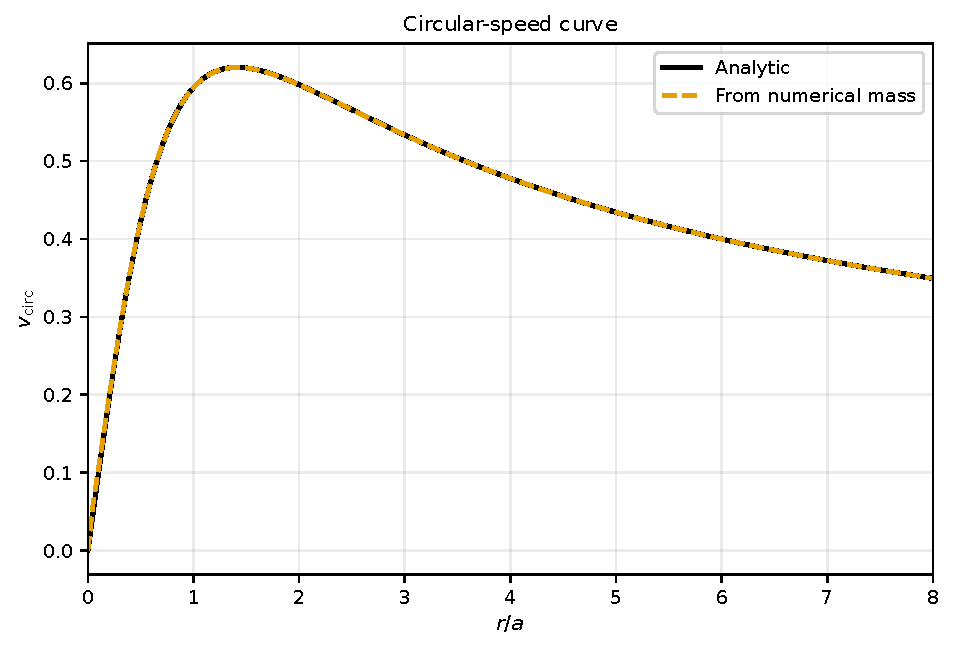
\includegraphics[width=0.68\linewidth]{ch01_circular_speed.pdf}
\caption{Plummer 球の回転曲線。縦軸は $v_\ast=\sqrt{GM/a}$ を単位としている。数値積分で得た内包質量から計算した回転曲線は解析式とよく一致する。解析的な最大位置は $r=\sqrt{2}a$ である。}
\label{fig:ch1-circular-speed}
\end{figure}

\begin{topicblock}{高次元の積分とモンテカルロ積分}
ここまでで、本章で扱う1次元数値積分とその物理的応用は完結した。
最後に、積分の次元が高くなると計算量と誤差の関係がどのように変わるかを簡単に見ておく。

本章では、積分区間を格子に分け、台形則や Simpson 則で1次元の定積分を求めた。
1次元で誤差が $h^p$ で減る積分公式では、滑らかな関数に対して格子を細かくするほど急速に精度が上がる。

一方、$d$ 次元の積分で各方向を $n$ 分割すると、総評価点数はおよそ $N_{\rm eval}=n^d$ になる。
1次元の積分公式を各方向に同じように適用すると、$h\sim N_{\rm eval}^{-1/d}$ なので、誤差はおおよそ
\[
 \epsilon\sim N_{\rm eval}^{-p/d}
\]
で減る。したがって、次元が高くなるほど、同じ評価点数で得られる精度は低下する。

これに対して、積分領域から無作為に点を選び、被積分関数の平均値から積分値を推定する方法を
\textbf{モンテカルロ積分（Monte Carlo integration）}という。区間 $[x_{\min},x_{\max}]$ では
\[
 I=\int_{x_{\min}}^{x_{\max}} f(x)\,dx
 \simeq
 \frac{x_{\max}-x_{\min}}{N_{\rm samp}}\sum_{k=1}^{N_{\rm samp}}f(x_k)
\]
と見積もる。ここで $x_k$ は区間内から独立に、一様に選んだ点であり、$N_{\rm samp}$ はサンプル数である。
被積分関数の分散が有限なら、この推定値の標準誤差は $N_{\rm samp}^{-1/2}$ に比例して減り、その指数は積分の次元に直接依存しない。
したがって、1次元の滑らかな積分では本章の方法のほうがはるかに効率的である。
一方、次元が高い場合や積分領域の形が複雑な場合には、モンテカルロ積分が有力な選択肢になる。
天文学では、輻射輸送でも乱数によるサンプリングが利用されている\cite{matsumoto}。

重力多体系シミュレーションで、等質量粒子の初期位置を作るときにも、乱数と内包質量を使う。
球対称分布の全質量を $M$ とし、$0<X<1$ の一様乱数を生成して $M(<r)/M=X$ を満たす半径 $r$ を求める。
この操作を\textbf{逆関数法（inverse transform sampling）}という。
半径の確率密度は $\rho(r)$ そのものではなく $4\pi r^2\rho(r)/M$ であり、方向も等方的に選ぶことで、密度分布 $\rho(r)$ に対応する粒子配置を作れる。
Plummer 球では式\eqref{eq:ch1-plummer-mass-exact}を逆に解き、
\[
 r=a\left(X^{-2/3}-1\right)^{-1/2}
\]
と求められる。
一般の密度分布では、累積積分で得た内包質量の表を逆にたどり、必要に応じて補間して半径を決める。
有限半径 $r_{\max}$ までの表を使う場合は、その半径までの質量で規格化し、$M(<r)=X M(<r_{\max})$ を満たす半径を求める。
これは位置分布の作成であり、平衡な初期条件を作るには、質量分布と整合する速度分布も別途与える必要がある。
粒子を独立に抽出すると、一定の半径内に入る粒子数の割合には統計的なゆらぎが残る。
その標準偏差は粒子数 $N_{\rm p}$ に対して $N_{\rm p}^{-1/2}$ に比例する。
これは乱数サンプリングのゆらぎであり、累積積分の離散化誤差や、その後の時間積分の誤差とは区別する。

詳しくは、乱数とモンテカルロ法は三井田・須田\cite{miida2023}第9章、
重力多体系の計算は富阪ほか編\cite{tomisaka2007}第6章を参照すること。
\end{topicblock}


\chapter{Poisson 方程式と有限差分法}
\label{chap:poisson-fd}

第1章では、球対称な密度分布を数値積分して重力場を求めた。
本章では、重力ポテンシャルを介して同じ重力場を求める過程を通して、境界値問題の数値解法と数値微分を学ぶ。

基本となる手法は、格子点上の関数値の差を用いて微分を近似する\textbf{有限差分法（finite-difference method）}である。
この考え方は、さまざまな常微分方程式や偏微分方程式に適用できる。
本章で Poisson 方程式を取り上げるのは、離散化、境界条件の組み込み、連立一次方程式の構成、数値解の検証を、解析解の分かる重力モデルで学べるためである。
実際の重力計算法は質量分布の表現や計算の目的によって異なるが\footnote{重力計算法の使い分けは、付録\ref{app:axisym-poisson}の補足「シミュレーション天文学で使う重力計算法」で紹介する。}、ここでは手順を追いやすい有限差分法を用い、1次元の境界値問題として解く。
さらに、得られたポテンシャルから重力加速度を求めるため、前進差分・後退差分・中心差分による\textbf{数値微分（numerical differentiation）}を行い、それぞれの精度を収束試験で比較する。

\begin{learningbox}[本章で学ぶこと]
\begin{itemize}
 \item 球対称 Poisson 方程式を、変数変換 $u=r\Phi$ により有限区間上の1次元境界値問題として設定できる。
 \item 二階微分を中心差分で近似し、中心と外側の境界条件を組み込んだ三重対角の連立一次方程式 $A\boldsymbol{u}=\boldsymbol{b}$ を構成できる。
 \item 前進差分・後退差分・中心差分を Taylor 展開から導き、数値微分に適用できる。
 \item 解析解との比較と格子収束試験から、境界値問題の数値解と数値微分の誤差・収束次数を評価できる。
 \item 連立一次方程式の残差と離散化誤差を区別し、残差が小さくても元の微分方程式に対する誤差が残る理由を説明できる。
\end{itemize}
\end{learningbox}



% =====================================================================
\section{Plummer 球の重力を求める二つの方法}
\label{sec:ch2-plummer}

第1章と同じ Plummer 密度分布
\begin{equation}
 \rho(r)=\frac{3M}{4\pi a^3}\left(1+\frac{r^2}{a^2}\right)^{-5/2}
\label{eq:ch2-plummer-density}
\end{equation}
を使う\cite{ryden2025}。

密度分布から重力ポテンシャル $\Phi$ を求めるには、両者を結ぶ Poisson 方程式
\begin{equation}
 \nabla^2\Phi=4\pi G\rho
\end{equation}
を、適切な境界条件のもとで解く。
球対称系では、得られたポテンシャル $\Phi(r)$ の微分から、重力加速度の動径成分を $g_r(r)=-d\Phi/dr$ と求められる。
ここでは動径方向の外向きを正とする。

Plummer 球では、ポテンシャルと重力加速度の解析式が分かっているため、数値計算の結果を直接検証できる。
無限遠でポテンシャルが0になるように基準を選び、$\Phi(\infty)=0$ とすると、
\begin{equation}
 \Phi_{\rm exact}(r)=-\frac{GM}{\sqrt{r^2+a^2}}
\label{eq:ch2-plummer-potential}
\end{equation}
である。
この式を微分すると、重力加速度は次のように求められる。
\begin{equation}
 g_{r,\rm exact}(r)=-\frac{d\Phi_{\rm exact}}{dr}=-\frac{GMr}{(r^2+a^2)^{3/2}}
\label{eq:ch2-plummer-gravity}
\end{equation}

また、式\eqref{eq:ch1-plummer-mass-exact}で得た内包質量
\begin{equation}
 M(<r)
 =M\frac{(r/a)^3}{[1+(r/a)^2]^{3/2}}
\label{eq:ch2-plummer-mass}
\end{equation}
からも、球対称性を使って
\begin{equation}
 g_r(r)=-\frac{GM(<r)}{r^2}
\label{eq:ch2-gravity-from-mass}
\end{equation}
と求められる。

したがって Plummer 球では、同じ $g_r$ を
\begin{equation}
 \rho\rightarrow M(<r)\rightarrow g_r,
 \qquad
 \rho\rightarrow\Phi\rightarrow g_r
\label{eq:ch2-three-routes}
\end{equation}
という二つの方法で計算でき、それぞれを解析解 $g_{r,\rm exact}$ と比較できる。
同じ物理量を独立した方法で求めて比較することは、数値計算を検証するうえで有用である。
数値積分、Poisson 方程式の求解、数値微分を組み合わせた比較は、Notebook 2 の「密度 $\rightarrow$ ポテンシャル $\rightarrow$ 重力」の計算例で示す。

\begin{notebookblock}{2｜Plummer 球}
Notebook では $G=M=a=1$ の無次元単位を用いる。
密度と内包質量には式\eqref{eq:ch2-plummer-density}、\eqref{eq:ch2-plummer-mass}を、ポテンシャルと重力加速度には式\eqref{eq:ch2-plummer-potential}、\eqref{eq:ch2-plummer-gravity}を使い、検証用の関数として定義する。

{\sffamily\small\color{graytext}対応セル（計算部分）}
\begin{Verbatim}[xleftmargin=2mm,fontsize=\small,frame=single,framesep=1.8mm,framerule=0.35pt,rulecolor=\color{listingframe},fillcolor=\color{listingbg}]
# 無次元単位を設定する
G = 1.0
M = 1.0
a = 1.0

# Plummer 球の密度と解析解
def rho_plummer(r, M, a):
    return 3.0 * M / (4.0 * np.pi * a**3) * (1.0 + (r / a)**2)**(-2.5)

def mass_plummer_exact(r, M, a):
    s = r / a
    return M * s**3 / (1.0 + s**2)**1.5

def phi_plummer_exact(r, G, M, a):
    return -G * M / np.sqrt(r**2 + a**2)

def gravity_plummer_exact(r, G, M, a):
    return -G * M * r / (r**2 + a**2)**1.5
\end{Verbatim}
\end{notebookblock}

% =====================================================================
\section{球対称 Poisson 方程式の1次元化}
\label{sec:ch2-spherical-poisson}

前節で示した Poisson 方程式を球対称系で考える。
球対称なら、密度とポテンシャルは半径 $r$ だけの関数となり、
Poisson 方程式は
\begin{equation}
 \frac{1}{r^2}\frac{d}{dr}
 \left(r^2\frac{d\Phi}{dr}\right)
 =4\pi G\rho(r)
\label{eq:ch2-poisson-spherical}
\end{equation}
と書ける。
したがって、3次元の偏微分方程式は、半径 $r$ だけを独立変数とする二階の常微分方程式へ帰着する。

式\eqref{eq:ch2-poisson-spherical}の左辺を展開すると
\begin{equation}
 \frac{d^2\Phi}{dr^2}
 +\frac{2}{r}\frac{d\Phi}{dr}
 =4\pi G\rho(r)
\end{equation}
である。
この形でも離散化できるが、$r=0$ では $2/r$ の係数をそのまま扱えない。
そこで、球対称 Poisson 方程式をより単純な形にするため、
\begin{equation}
 u(r)\equiv r\Phi(r)
\label{eq:ch2-u-def}
\end{equation}
を導入する。以下、プライムは $r$ に関する微分を表す。
$r>0$ では $\Phi=u/r$ なので、
\begin{align}
 \frac{d\Phi}{dr}
 &=\frac{u'}{r}-\frac{u}{r^2},\\
 r^2\frac{d\Phi}{dr}
 &=ru'-u,\\
 \frac{d}{dr}\left(r^2\frac{d\Phi}{dr}\right)
 &=ru''
\end{align}
となる。
この結果を式\eqref{eq:ch2-poisson-spherical}に代入し、$r>0$ で両辺に $r$ を掛けると、
\begin{equation}
 \frac{d^2u}{dr^2}=4\pi G r\rho(r)
\end{equation}
を得る。
さらに、右辺を
\begin{equation}
 s(r)\equiv4\pi G r\rho(r)
\label{eq:ch2-source-def}
\end{equation}
と書けば、
\begin{equation}
\boxed{
 u''(r)=s(r)
 }
\label{eq:ch2-u-poisson}
\end{equation}
となる。
変数変換 $u=r\Phi$ によって、球対称座標に由来する $1/r$ を含む係数が消え、
左辺は単純な二階微分だけになった。
このため、次節では $u''$ を中心差分で近似することで、内部格子点の方程式を直接構成できる。

式\eqref{eq:ch2-u-poisson}は二階の常微分方程式であり、解を定めるには二つの独立な条件が必要である。
本章では $0\le r\le r_{\max}$ を計算領域とし、その両端で $u$ の値を指定する。
微分方程式に加えて、境界で与えた条件を満たす解を求めることになる。

\begin{definitionbox}{境界値問題}
微分方程式と、計算領域の境界で与える条件を組み合わせて解を求める問題を
\textbf{境界値問題（boundary-value problem）}と呼ぶ。
\end{definitionbox}

中心と外側で具体的に与える境界値は、§\ref{sec:ch2-boundaries}で説明する。

% =====================================================================
\section{Poisson 方程式の中心差分による離散化}
\label{sec:ch2-second-difference}

式\eqref{eq:ch2-u-poisson}では、未知量は半径 $r$ の連続関数 $u(r)$ である。
数値計算では、計算領域を有限個の格子点に分け、
各格子点での関数値を未知数として求める。
そのため、微分方程式に含まれる微分を、
格子点上の有限個の関数値を用いて近似する。

この置き換えによって、連続な微分方程式は、
有限個の未知数に対する代数方程式へ近似的に置き換えられる。
本章で扱う Poisson 方程式は線形なので、
内部格子点で得られる差分方程式と境界条件をまとめると、
連立一次方程式として数値解を求めることができる。
このように、連続な問題を有限個の未知数からなる問題へ置き換えることを
\textbf{離散化（discretization）}という。

ここでは、二階微分 $u''$ を中心差分で近似して、
式\eqref{eq:ch2-u-poisson}を離散化する。
計算領域 $0\le r\le r_{\max}$ を $N$ 個の区間に等分し、
\begin{equation}
 r_i=i\Delta r,
 \qquad
 \Delta r=\frac{r_{\max}}{N},
 \qquad i=0,1,\ldots,N
\label{eq:ch2-grid}
\end{equation}
という等間隔格子を導入する。
格子点は $N+1$ 個である。
滑らかな関数 $u(r)$ の格子点での値を $u_i=u(r_i)$ とし、
$u_i'=u'(r_i)$ などと書く。

内部格子点 $r_i$ のまわりで $u_{i\pm1}=u(r_i\pm\Delta r)$ を Taylor 展開すると、
\begin{align}
 u_{i+1}&=u_i+\Delta r\,u_i'+\frac{(\Delta r)^2}{2}u_i''+\frac{(\Delta r)^3}{6}u_i'''+O((\Delta r)^4),\\
 u_{i-1}&=u_i-\Delta r\,u_i'+\frac{(\Delta r)^2}{2}u_i''-\frac{(\Delta r)^3}{6}u_i'''+O((\Delta r)^4)
\end{align}
である。
2式を足して $2u_i$ を引くと、表示した1次と3次の項が消え、
\begin{equation}
 u_{i+1}-2u_i+u_{i-1}=(\Delta r)^2u_i''+O((\Delta r)^4)
\end{equation}
となる。
両辺を $(\Delta r)^2$ で割ると、
\begin{equation}
 \frac{u_{i+1}-2u_i+u_{i-1}}{(\Delta r)^2}=u_i''+O((\Delta r)^2)
\end{equation}
を得る。
したがって、二階微分は
\begin{equation}
 \boxed{u_i''\simeq\frac{u_{i+1}-2u_i+u_{i-1}}{(\Delta r)^2}}
\label{eq:ch2-second-central}
\end{equation}
と近似できる。
これが二階微分の3点中心差分であり、この近似の打ち切り誤差は $O((\Delta r)^2)$ である。

次に、この中心差分を式\eqref{eq:ch2-u-poisson}へ代入し、
各内部格子点で数値近似が満たす方程式を作る。
ここまでの Taylor 展開では $u_i=u(r_i)$ を厳密な格子点値として用いたが、
以下では記号を簡単にするため、格子点 $r_i$ における数値近似も $u_i$ と書く。
また、既知の右辺を $s_i=s(r_i)$ とする。
各内部格子点では
\begin{equation}
 \frac{u_{i+1}-2u_i+u_{i-1}}{(\Delta r)^2}=s_i
\end{equation}
となる。
後で係数行列の対角成分を正に書くため、両辺に $-(\Delta r)^2$ を掛けると、
\begin{equation}
 \boxed{
 -u_{i-1}+2u_i-u_{i+1}
 =-(\Delta r)^2s_i
 }
\label{eq:ch2-discrete-poisson}
\end{equation}
を得る。

ここで、差分公式がどの格子点を使っているかを整理しておく。

\begin{definitionbox}{差分ステンシル}
ある格子点の差分式を構成するために用いる格子点の組を、
\textbf{差分ステンシル（finite-difference stencil）}と呼ぶ。
本節の二階中心差分では $r_{i-1},r_i,r_{i+1}$ の3点を使うため、
式\eqref{eq:ch2-discrete-poisson}は3点ステンシルである
（図\ref{fig:ch2-stencil}）。
\end{definitionbox}

\begin{figure}[!htbp]
\centering
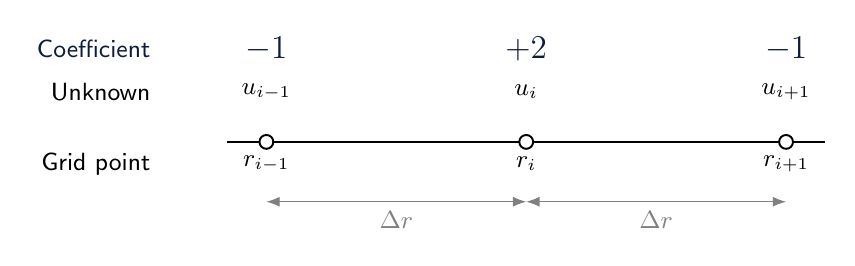
\begin{tikzpicture}[>=Latex,font=\sffamily\small]
 \node[anchor=east,text=navy] at (-0.15,1.18) {Coefficient};
 \node[anchor=east] at (-0.15,0.64) {Unknown};
 \node[anchor=east] at (-0.15,-0.28) {Grid point};
 \draw[thick] (0.7,0)--(8.3,0);
 \foreach \x/\rlab/\ulab/\coef in {1.2/{r_{i-1}}/{u_{i-1}}/{-1},4.5/{r_i}/{u_i}/{+2},7.8/{r_{i+1}}/{u_{i+1}}/{-1}}{
   \filldraw[fill=white,line width=0.7pt] (\x,0) circle (2.5pt);
   \node at (\x,-0.28) {$\rlab$};
   \node at (\x,0.64) {$\ulab$};
   \node[text=navy,font=\large] at (\x,1.18) {$\coef$};
 }
 \draw[<->,gray] (1.2,-0.76)--node[below]{$\Delta r$}(4.5,-0.76);
 \draw[<->,gray] (4.5,-0.76)--node[below]{$\Delta r$}(7.8,-0.76);
\end{tikzpicture}
\caption{式\eqref{eq:ch2-discrete-poisson}の3点ステンシル。上段は左辺における $u_{i-1},u_i,u_{i+1}$ の係数である。二階微分の中心差分そのものの係数 $1,-2,1$ ではなく、式\eqref{eq:ch2-discrete-poisson}で用いる係数 $-1,2,-1$ を示している。}
\label{fig:ch2-stencil}
\end{figure}

% =====================================================================

\section{中心と外側の境界条件}
\label{sec:ch2-boundaries}

前節で得た内部格子点の差分式に加えて、計算領域の両端で境界条件を与える。
本章では $0\le r\le r_{\max}$ で式\eqref{eq:ch2-u-poisson}を解くため、中心 $r=0$ と外側 $r=r_{\max}$ の値を指定する。

\subsection{中心境界条件と $\Phi(0)$ の復元}

中心でポテンシャル $\Phi(0)$ が有限なら、
$u=r\Phi$ なので
\begin{equation}
 u(0)=0
\label{eq:ch2-u0}
\end{equation}
である。
したがって、$u$ について Poisson 方程式を解くときの中心境界条件は
\begin{equation}
 u_0=0
\end{equation}
と与えればよい。

一方、Poisson 方程式を解いた後で $u$ からポテンシャル $\Phi$ を復元するときには、
中心だけ別の扱いが必要になる。
$r_i>0$ では
\begin{equation}
 \Phi_i=\frac{u_i}{r_i}
\end{equation}
とすればよいが、中心では $u_0=r_0=0$ なので、
この式は $0/0$ となり直接使えない。
これは $u$ の中心境界条件に問題があるのではなく、
変数変換 $u=r\Phi$ から $\Phi$ に戻すときに生じるものである。

中心でポテンシャルが滑らかなら
\begin{equation}
 \Phi(0)
 =\lim_{r\to0}\frac{u(r)}{r}
 =u'(0)
\label{eq:ch2-center-limit}
\end{equation}
である。
この滑らかさと球対称性による中心まわりの対称性を用いると、
中心値 $\Phi_0=\Phi(0)$ は中心近傍の2点から
\begin{equation}
 \boxed{
 \Phi_0
 \simeq
 \frac{4\Phi_1-\Phi_2}{3}
 }
\label{eq:ch2-center-phi}
\end{equation}
と近似できる（「補足｜中心ポテンシャルの外挿公式の導出」を参照）。
実際に Poisson 方程式で求める未知数は $u$ なので、
$\Phi_1=u_1/\Delta r$、
$\Phi_2=u_2/(2\Delta r)$ を代入すると
\begin{equation}
 \boxed{
 \Phi_0
 \simeq
 \frac{8u_1-u_2}{6\Delta r}
 }
\label{eq:ch2-center-u}
\end{equation}
となる。数値計算では、この式を用いて中心ポテンシャルを復元する。

\begin{topicblock}{中心ポテンシャルの外挿公式の導出}
中心を通る任意の直線上に、中心を $\ell=0$ とする符号付き座標 $\ell$ を取る。
球対称性から、中心から同じ距離にある $\ell$ と $-\ell$ では
ポテンシャルが等しいので、
\begin{equation}
 \Phi(\ell)=\Phi(-\ell)
\end{equation}
が成り立つ。
中心で $\Phi$ が滑らかなら $\Phi$ は $\ell$ の偶関数であり、
中心まわりの Taylor 展開には偶数次の項だけが現れる。
半径 $r=|\ell|$ を用いると
\begin{equation}
 \Phi(r)=\Phi_0+c_2r^2+c_4r^4+O(r^6)
\end{equation}
と書ける。

$r_1=\Delta r$、$r_2=2\Delta r$ とすると
\begin{align}
 \Phi_1&=\Phi_0+c_2(\Delta r)^2+c_4(\Delta r)^4+O((\Delta r)^6),\\
 \Phi_2&=\Phi_0+4c_2(\Delta r)^2+16c_4(\Delta r)^4+O((\Delta r)^6).
\end{align}
ここで $4\Phi_1-\Phi_2$ を作ると $(\Delta r)^2$ の項が消え、
\begin{equation}
 \frac{4\Phi_1-\Phi_2}{3}
 =\Phi_0-4c_4(\Delta r)^4+O((\Delta r)^6)
\end{equation}
となる。
したがって、
\begin{equation}
 \Phi_0
 =\frac{4\Phi_1-\Phi_2}{3}
 +O((\Delta r)^4)
\end{equation}
を得る。
さらに
$\Phi_1=u_1/\Delta r$、
$\Phi_2=u_2/(2\Delta r)$ を代入すると、
式\eqref{eq:ch2-center-u}が得られる。

ただし、この $O((\Delta r)^4)$ は、
$\Phi_1,\Phi_2$ が厳密に分かっている場合の外挿誤差である。
実際には、これらも有限差分法で求めた近似値であり、
誤差を含むため、中心ポテンシャルが4次精度で求まるとは限らない。
\end{topicblock}


\subsection{外側境界条件}

もう一つの境界条件は、計算領域の外側 $r=r_{\max}$ に与える。
まず有限差分法そのものの精度を検証するため、
本章の Plummer 球では解析解を用いて
\begin{equation}
 u_N
 =r_{\max}\Phi_{\rm exact}(r_{\max})
\label{eq:ch2-outer-exact}
\end{equation}
とする。
これにより、外側境界の近似による誤差を入れずに、
主として有限差分による離散化誤差を調べることができる。

解析解が分からなくても、全質量 $M$ が有限な孤立系では、
十分遠方で質量分布を点質量として近似し、
\begin{equation}
 \Phi(r)\simeq-\frac{GM}{r},
 \qquad
 u(r)\simeq-GM
\label{eq:ch2-outer-pointmass}
\end{equation}
を外側境界条件として用いることができる。
ただし、本章の Plummer 球は $r_{\max}$ より外側にも広がっているため、
有限の $r_{\max}$ でこの近似を境界値に用いると、解析値との差が生じる。
この誤差は有限差分の離散化誤差とは別のものであり、
$r_{\max}$ を十分大きく取るか、より適切な外側境界条件を用いることで小さくする必要がある。
この影響の計算例は Notebook 2 の「境界条件による誤差」に示す。

本章では、有限の計算領域で Poisson 方程式を解くために、外側境界でポテンシャルの値を与えた。
自己重力を含む数値シミュレーションでも、密度分布から重力ポテンシャルを
有限の計算領域上で求める場合には、外側境界条件を指定する必要がある\footnote{
質量分布が境界より十分内側に収まる場合には、点質量による項を先頭とし、非球対称な分布の効果を高次の項で表す
\textbf{多重極展開（multipole expansion）}を用いることがある\cite{tomisaka2007}。
これは質量配置の近似を改良する方法であり、境界より外側の質量を無視したことによる誤差とは区別する。
}。


\begin{topicblock}{孤立系の境界条件と James 法}
本章では Plummer 球の解析解が分かるため、外側境界のポテンシャルを直接与えられる。
一方、一般の非球対称な質量分布では、有限の計算領域の境界上で
どのようなポテンシャルを与えるかが問題になる。
孤立系では無限遠で $\Phi\to0$ となるが、
有限の距離にある境界で単に $\Phi=0$ としても、一般には正しい解にならない。

James 法（James 1977）は、孤立系の境界条件を有限の計算領域で扱う方法である\cite{james1977,bt2008}。
まず、境界上でポテンシャルを0と仮定して Poisson 方程式を解く。
しかし、この仮定は実際の孤立系の境界条件とは異なる。
そこで、境界を0としたことで生じる影響を計算して取り除き、
孤立系に対応するポテンシャルを求める。

James 法は有限差分法を置き換えるものではなく、
Poisson 方程式の数値解法と組み合わせて境界条件を扱う方法である。
ただし、計算領域の外側にも質量がある場合は、その寄与を別途考慮する必要がある。
\end{topicblock}

% =====================================================================
\section{連立一次方程式の組み立て}
\label{sec:ch2-matrix}

式\eqref{eq:ch2-discrete-poisson}には、格子点 $r_i$ における
$u_i$ だけでなく、隣の格子点の値 $u_{i-1}$ と $u_{i+1}$ も含まれる。
したがって、各 $u_i$ を独立に求めることはできず、
すべての内部格子点の差分式をまとめて連立一次方程式として解く必要がある。

まず、差分式がどのような連立一次方程式になるかを見るため、
$r_0,r_1,r_2,r_3,r_4$ の5個の格子点だけを持つ簡単な例を考える。
両端の $r_0,r_4$ は境界点であり、$r_1,r_2,r_3$ は内部格子点である。
この例では、左境界に隣接する $r_1$、両隣が内部点である $r_2$、
右境界に隣接する $r_3$ の3種類の差分式を確認できる。

この例では、両端の $u_0$ と $u_4$ は境界条件によって与えられる。
したがって、求める未知数は内部3点の
\begin{equation}
 u_1,\quad u_2,\quad u_3
\end{equation}
である。
式\eqref{eq:ch2-discrete-poisson}を
$r_1,r_2,r_3$ にそれぞれ適用すると、
\begin{align}
 2u_1-u_2
 &=-(\Delta r)^2s_1+u_0,\\
 -u_1+2u_2-u_3
 &=-(\Delta r)^2s_2,\\
 -u_2+2u_3
 &=-(\Delta r)^2s_3+u_4.
\end{align}
これら3本の式をまとめると、
\begin{equation}
 \begin{pmatrix}
 2&-1&0\\
 -1&2&-1\\
 0&-1&2
 \end{pmatrix}
 \begin{pmatrix}u_1\\u_2\\u_3\end{pmatrix}
 =
 \begin{pmatrix}
 -(\Delta r)^2s_1+u_0\\
 -(\Delta r)^2s_2\\
 -(\Delta r)^2s_3+u_4
 \end{pmatrix}
\label{eq:ch2-small-matrix}
\end{equation}
となる。

ここで、左端の行列を係数行列 $A$、
内部格子点の未知数を並べた列ベクトルを $\boldsymbol{u}$、
既知の量をまとめた右辺の列ベクトルを $\boldsymbol{b}$ と書くと、
式\eqref{eq:ch2-small-matrix}は
\begin{equation}
 A\boldsymbol{u}=\boldsymbol{b}
\label{eq:ch2-linear-system}
\end{equation}
と簡潔に表せる。
一般の $N$ では、
\begin{equation}
 \boldsymbol{u}
 =
 \begin{pmatrix}
 u_1&u_2&\cdots&u_{N-1}
 \end{pmatrix}^{\mathsf T}
\end{equation}
が求める未知数ベクトルである。上付きの $\mathsf{T}$ は転置を表し、横に並べた成分を列ベクトルにしている。
係数行列 $A$ の非零成分は、主対角とその上下の対角にだけ現れる。
このような行列を
\textbf{三重対角行列（tridiagonal matrix）}と呼ぶ。

Listing 2.1 に、一般の $N$ に対して
係数行列 $A$ と右辺ベクトル $\boldsymbol{b}$ を組み立てる部分を示す。

\begin{listingbox}{2.1　三重対角行列と境界値の組み込み}
\begin{Verbatim}[fontsize=\small]
# 内部格子点の値 u_1, ..., u_{N-1} を未知数とする
n = N - 1
A = np.zeros((n, n))

# 三重対角行列の係数 (-1, 2, -1) を入れる
np.fill_diagonal(A, 2.0)
np.fill_diagonal(A[1:], -1.0)
np.fill_diagonal(A[:, 1:], -1.0)

# 内部格子点に対応する右辺ベクトルを作る
b = -(dr**2) * source[1:N].copy()

# 既知の境界値 u_0, u_N を右辺へ組み込む
b[0] += u0
b[-1] += uN
\end{Verbatim}
\end{listingbox}

一般の格子では、未知数は $u_1,\ldots,u_{N-1}$ の $N-1$ 個である。
コード中の \texttt{n = N - 1} はこの未知数の数を表す。
また、\texttt{dr} は格子幅 $\Delta r$、
\texttt{source[1:N]} は内部格子点の
$s_1,\ldots,s_{N-1}$ を取り出している。
係数行列 $A$ の主対角の $2$ と上下の副対角の $-1$ は、
式\eqref{eq:ch2-discrete-poisson}の左辺の係数に対応する。

5格子点の例と同様に、一般の $N$ 区間でも、
両端の境界値 $u_0$ と $u_N$ は未知数に含めず、右辺に組み込む。
コード中の \texttt{b[0] += u0} は、
最初の内部格子点 $r_1$ の式に中心境界値 $u_0$ を加える操作に対応する。
同様に、\texttt{b[-1] += uN} は、
最後の内部格子点 $r_{N-1}$ の式に外側境界値 $u_N$ を加える操作である。
本章では $u_0=0$ なので最初の加算は値を変えないが、
差分式とコードの対応を明示するために残している。


% =====================================================================

\section{Plummer 球の Poisson 方程式の数値解}
\label{sec:ch2-solve-plummer}

ここまで、球対称 Poisson 方程式を有限差分法で解くために、
球対称性による1次元化と変数変換、中心差分による離散化、境界条件の設定、
連立一次方程式の組み立てを順に説明してきた。
本節では、これらの手順をまとめて Plummer 球に適用し、
重力ポテンシャルを数値的に求める。

\medskip
\noindent\textbf{計算手順｜球対称 Poisson 方程式を有限差分で解く}
\par\smallskip
\begin{enumerate}[itemsep=0em,topsep=0.1em]
 \item $r_i=i\Delta r$ の格子を作り、密度 $\rho_i=\rho(r_i)$ と
       右辺 $s_i=4\pi G r_i\rho_i$ を計算する。
 \item 中心境界 $u_0=0$ と外側境界 $u_N$ を与える。
 \item 内部格子点の差分式から、係数行列 $A$ と
       右辺ベクトル $\boldsymbol{b}$ を組み立てる。
 \item 連立一次方程式 $A\boldsymbol{u}=\boldsymbol{b}$ を解き、
       $u_1,\ldots,u_{N-1}$ を求める。
 \item 境界値と内部の数値解を合わせて $u_i$ を構成し、
       $r_i>0$ では $\Phi_i=u_i/r_i$ とする。
       中心値 $\Phi_0$ は式\eqref{eq:ch2-center-u}から復元する。
\end{enumerate}
\medskip

以下では、この一連の手順を Python で実行する。
連立一次方程式の求解には、NumPy の \texttt{np.linalg.solve} を使う。\footnote{一般の密行列には Gauss の消去法や LU 分解が用いられる。本章のような三重対角行列では、構造を利用した Thomas 法によって計算量を $O(N)$ にできる。これらの解法の基本的な考え方は付録\ref{app:linear-systems}、詳しい説明は幸谷 第7章\cite{kouya2021}を参照。}

得られた数値解を検証するため、
ポテンシャルを同じ格子点で評価した解析解と比較する。
あわせて、連立一次方程式をどの程度満たしているかを残差で確認する。

\begin{definitionbox}{残差}
連立一次方程式 $A\boldsymbol{u}=\boldsymbol{b}$ に数値解を代入したときの左右のずれ
\begin{equation}
 \boldsymbol{r}_{\rm res}
 =A\boldsymbol{u}-\boldsymbol{b}
\label{eq:ch2-residual}
\end{equation}
を\textbf{残差（residual）}という。
残差は、数値解が離散化した連立一次方程式をどの程度満たしているかを表す。
残差が小さくても、解析解との誤差が小さいとは限らない。
\end{definitionbox}

\begin{notebookblock}{2｜Poisson 方程式の数値解}
Notebook では、一連の計算手順を関数
\texttt{solve\_\allowbreak spherical\_\allowbreak poisson\_\allowbreak plummer} にまとめる。
関数の内部では、格子と右辺の作成、境界条件の設定、
連立一次方程式の組み立てと求解、$u$ から $\Phi$ への復元を順に行う。
外側境界は引数 \texttt{boundary} で選び、
本節では式\eqref{eq:ch2-outer-exact}の解析的な境界条件を用いる。

{\sffamily\small\color{graytext}対応セル（関数定義）}
\begin{Verbatim}[xleftmargin=2mm,fontsize=\small,frame=single,framesep=1.8mm,framerule=0.35pt,rulecolor=\color{listingframe},fillcolor=\color{listingbg}]
def solve_spherical_poisson_plummer(N, r_max, G, M, a, boundary="exact"):
    # 1. 格子を作り、密度と Poisson 方程式の右辺を計算する
    r = np.linspace(0.0, r_max, N + 1)
    dr = r[1] - r[0]
    rho = rho_plummer(r, M, a)
    source = 4.0 * np.pi * G * r * rho

    # 2. 中心境界と外側境界を与える
    u0 = 0.0
    if boundary == "exact":
        uN = r_max * phi_plummer_exact(r_max, G, M, a)
    elif boundary == "point_mass":
        uN = -G * M
    else:
        raise ValueError("boundary は 'exact' または 'point_mass' を指定")

    # 3. 係数行列 A と右辺ベクトル b を組み立てる
    n = N - 1
    A = np.zeros((n, n))
    np.fill_diagonal(A, 2.0)
    np.fill_diagonal(A[1:], -1.0)
    np.fill_diagonal(A[:, 1:], -1.0)

    b = -(dr**2) * source[1:N].copy()
    b[0] += u0
    b[-1] += uN

    # 4. A u = b を解き、境界値と内部解を合わせる
    u = np.empty(N + 1)
    u[0] = u0
    u[1:N] = np.linalg.solve(A, b)
    u[N] = uN

    # 5. u = r Phi からポテンシャルを復元する
    phi = np.empty(N + 1)
    phi[1:] = u[1:] / r[1:]
    phi[0] = (8.0 * u[1] - u[2]) / (6.0 * dr)

    return r, rho, u, phi, A, b
\end{Verbatim}

この関数が返す配列 \texttt{u} は、両端の境界値を含む $N+1$ 個の値からなる。
連立一次方程式の未知数ベクトル $\boldsymbol{u}$ に対応するのは、内部の $N-1$ 個を取り出した \texttt{u[1:N]} である。
この関数を $N=200$、$r_{\max}=10a$ で実行すると、$\Delta r=0.05a$ となる。
以下では、数値ポテンシャルの最大絶対誤差と、
残差の各成分の絶対値の最大値を計算する。

{\sffamily\small\color{graytext}対応セル（計算部分）}
\begin{Verbatim}[xleftmargin=2mm,fontsize=\small,frame=single,framesep=1.8mm,framerule=0.35pt,rulecolor=\color{listingframe},fillcolor=\color{listingbg}]
# 計算領域と区間数を設定する
N = 200
r_max = 10.0 * a

# Poisson 方程式を解いて数値ポテンシャルを得る
r, rho, u, phi_num, A, b = solve_spherical_poisson_plummer(
    N=N, r_max=r_max, G=G, M=M, a=a, boundary="exact"
)

# 同じ格子点で解析解を計算する
phi_exact = phi_plummer_exact(r, G, M, a)

# 離散方程式 A u = b の残差を確認する
residual = A @ u[1:N] - b

# ポテンシャルの最大誤差と最大残差
phi_error = np.max(np.abs(phi_num - phi_exact))
residual_max = np.max(np.abs(residual))
\end{Verbatim}
\end{notebookblock}

図\ref{fig:ch2-potential}では、数値ポテンシャルと解析解はほぼ重なり、
解析解をよく再現できていることが確認できる。

\begin{figure}[!htbp]
\centering
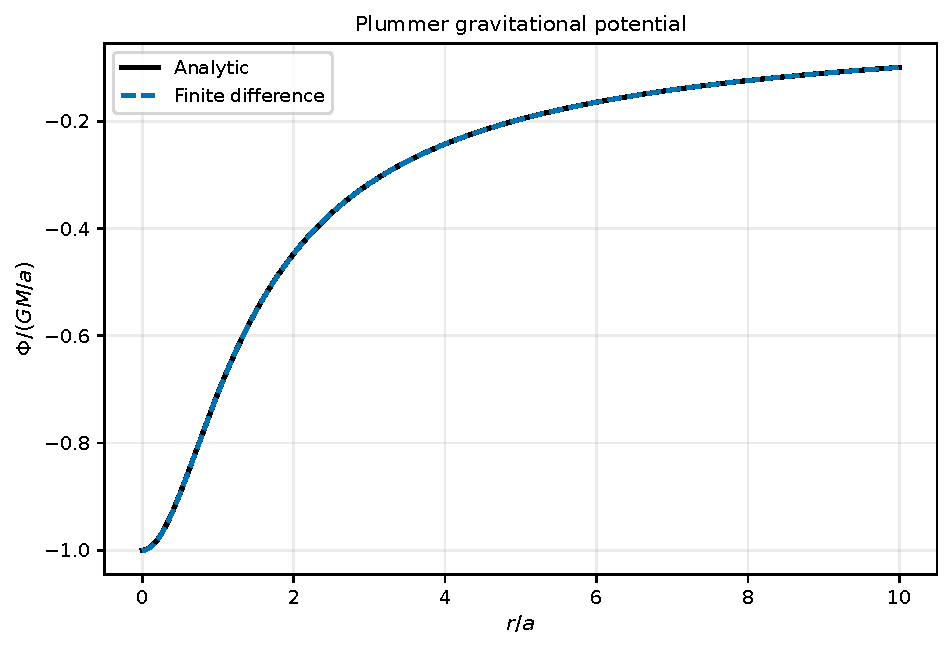
\includegraphics[width=0.68\linewidth]{ch02_potential.pdf}
\caption{Plummer ポテンシャルの有限差分解と解析解。}
\label{fig:ch2-potential}
\end{figure}

一方、差を拡大した図\ref{fig:ch2-potential-error}では、
有限差分による離散化誤差が確認できる。
今回の $N=200$ では、ポテンシャルの最大絶対誤差は
\begin{equation}
 \max_{0\le i\le N}|\Phi_{\rm num}(r_i)-\Phi_{\rm exact}(r_i)|
 =\chtwoPhiErrNTwoHundred\,\frac{GM}{a}
\label{eq:ch2-main-potential-error}
\end{equation}
である。
同じ計算を $G=M=a=1$ の無次元単位で行ったとき、連立一次方程式の最大残差は
$\max_i |(A\boldsymbol{u}-\boldsymbol{b})_i|\simeq3.85\times10^{-16}$ である。
残差の大きさは方程式の規格化に依存するが、今回用いた形では、左右のずれは浮動小数点演算の精度に近い大きさまで小さくなっている。
つまり、数値解は離散方程式 $A\boldsymbol{u}=\boldsymbol{b}$ を高い精度で満たしている。
それにもかかわらず解析解との差が残るのは、
$A\boldsymbol{u}=\boldsymbol{b}$ が Poisson 方程式そのものではなく、
二階微分を中心差分で近似して得られた離散方程式だからである。
このため、連立一次方程式を高い精度で解いても、
元の連続な Poisson 方程式に対する離散化誤差は残る。

\begin{figure}[!htbp]
\centering
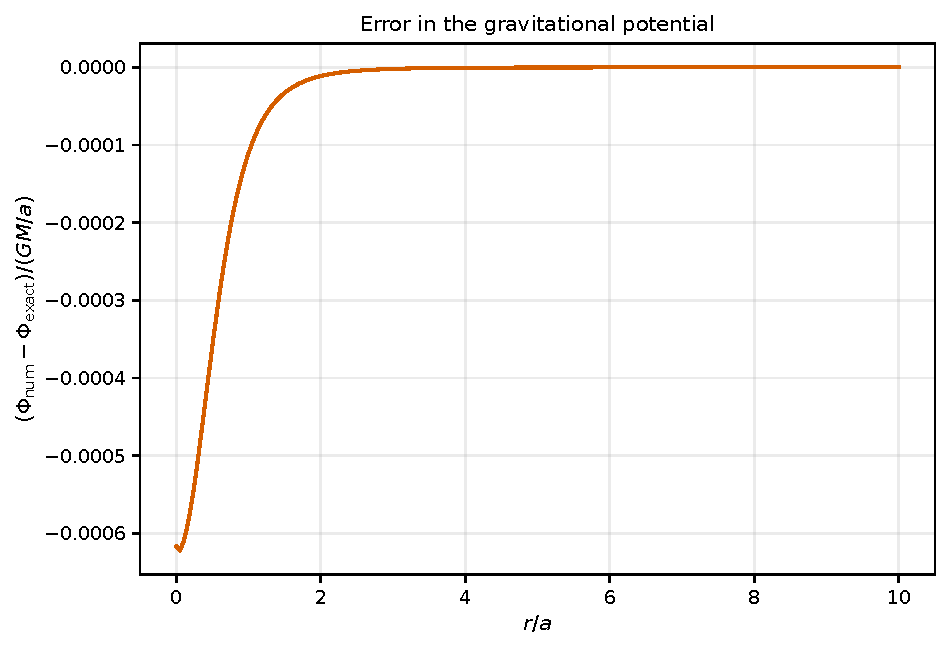
\includegraphics[width=0.68\linewidth]{ch02_potential_error.pdf}
\caption{有限差分で得た Plummer ポテンシャルの誤差。縦軸は符号付きの差 $(\Phi_{\rm num}-\Phi_{\rm exact})/(GM/a)$ であり、絶対値ではない。外側境界には解析解を与えている。}
\label{fig:ch2-potential-error}
\end{figure}


% =====================================================================
\section{Poisson 方程式の格子収束}
\label{sec:ch2-poisson-convergence}

前節では、$N=200$ の一つの格子について数値ポテンシャルを解析解と比較し、
有限差分による離散化誤差が残ることを確認した。
しかし、一つの格子で誤差を測るだけでは、
格子を細かくしたときに数値解がどのように解析解へ近づくかは分からない。
そこで本節では、格子幅 $\Delta r$ を変えて同じ計算を繰り返し、
ポテンシャルの誤差がどのように減少するかを調べる。
二階中心差分そのものの近似誤差は $O((\Delta r)^2)$ なので、
ポテンシャル全体の誤差についても2次収束が得られるかを
格子収束試験によって確認する。

計算領域は $r_{\max}=10a$ に固定し、
外側境界には前節と同じく解析値を与える。
そのうえで区間数を
\begin{equation}
 N=50,100,200,400,800
\label{eq:ch2-poisson-grids}
\end{equation}
と変化させる。
各格子では、ポテンシャルの最大絶対誤差を $GM/a$ で無次元化し、
\begin{equation}
 \epsilon_\Phi
 \equiv
 \max_{0\le i\le N}
 \frac{|\Phi_{\rm num}(r_i)-\Phi_{\rm exact}(r_i)|}{GM/a}
\label{eq:ch2-phi-error-def}
\end{equation}
として評価する。

\begin{notebookblock}{2｜Poisson 方程式の格子収束}
Notebook では5種類の格子で $\epsilon_\Phi$ を測り、両対数直線の傾きから収束次数を求める。

{\sffamily\small\color{graytext}対応セル（計算部分）}
\begin{Verbatim}[xleftmargin=2mm,fontsize=\small,frame=single,framesep=1.8mm,framerule=0.35pt,rulecolor=\color{listingframe},fillcolor=\color{listingbg}]
# 1つの格子でポテンシャルの最大誤差を測る
def poisson_error(N):
    r, _, _, phi_num, _, _ = solve_spherical_poisson_plummer(
        N=N, r_max=10.0 * a, G=G, M=M, a=a
    )
    phi_exact = phi_plummer_exact(r, G, M, a)
    dr = r[1] - r[0]
    err = np.max(np.abs(phi_num - phi_exact)) / (G * M / a)
    return dr, err

# 区間数を増やし、格子幅と誤差を記録する
N_values = np.array([50, 100, 200, 400, 800])
dr_values = []
phi_errors = []

for N_i in N_values:
    dr_i, err_i = poisson_error(int(N_i))
    dr_values.append(dr_i)
    phi_errors.append(err_i)

dr_values = np.array(dr_values)
phi_errors = np.array(phi_errors)

# log(error)-log(dr) の傾きが収束次数 p
order_phi = np.polyfit(
    np.log(dr_values), np.log(phi_errors), 1
)[0]
\end{Verbatim}
\end{notebookblock}

\begin{figure}[!htbp]
\centering
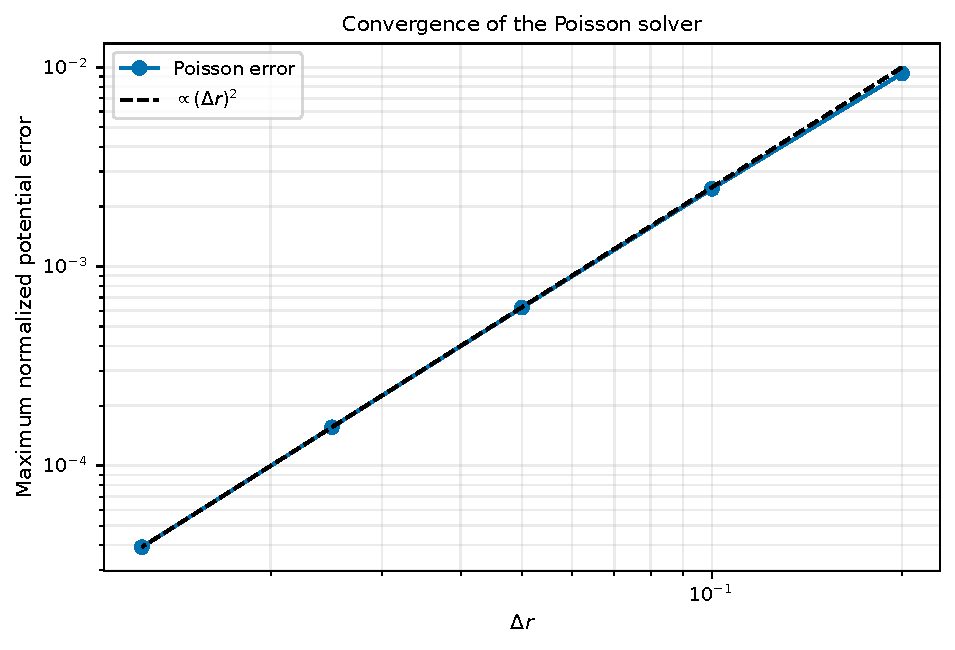
\includegraphics[width=0.68\linewidth]{ch02_poisson_convergence.pdf}
\caption{Poisson 方程式ソルバーの格子収束。破線は $\epsilon_\Phi\propto(\Delta r)^2$ を示す。}
\label{fig:ch2-poisson-convergence}
\end{figure}

5つの格子で得た誤差を両対数上で直線近似すると、$p=\chtwoPoissonOrder$ を得る。
$p$ はほぼ2であるため、ポテンシャルの数値解は格子幅 $\Delta r$ に対して2次精度で収束していることが分かる
（図\ref{fig:ch2-poisson-convergence}）。
すなわち、格子幅を半分にすると、誤差はおよそ $1/4$ に減少する。


% =====================================================================
\section{数値微分による重力加速度}
\label{sec:ch2-numerical-diff}

Poisson 方程式から $\Phi(r)$ が得られたら
\begin{equation}
 g_r(r)=-\frac{d\Phi}{dr}
\label{eq:ch2-g-from-phi}
\end{equation}
を数値微分で計算する。
ポテンシャルが格子上の値として与えられる場合には、差分して重力加速度を求める方法がある\cite{matsumoto}。
本節では、この計算を題材に数値微分の基本を学ぶ。
以下では前進差分（forward difference）、後退差分（backward difference）、中心差分（central difference）を Taylor 展開から導く\footnote{
ここでは3つの差分公式を紹介するが、内部の格子点では、同じく2点の値だけで2次精度が得られる中心差分を使うのが基本である。
前進・後退差分が必要になるのは、片側にしか格子点がない計算領域の端と、
時間方向のように一方向の値しか使えない場合である。後者の例が第3章の Euler 法である。
端点でも2次精度を保ちたい場合は、片側の3点を使う公式
$f'_0\simeq(-3f_0+4f_1-f_2)/(2\Delta r)$ がよく使われる。
ただし、流体の移流のように、流れの向きに応じて片側差分を選ばないと計算が不安定になる問題もあり、
中心差分が常に適しているわけではない。詳しくは藤井・立川\cite{fujii2020}、松本ほか\cite{matsumoto}を参照すること。}\cite{kouya2021}。
以下の $\Phi_i$ は、滑らかなポテンシャルを格子点 $r_i$ で評価した値を表す。まず差分公式自体の近似誤差を調べる。

\subsection{前進差分（forward difference）}

$r_i$ のまわりで
\begin{equation}
 \Phi_{i+1}
 =\Phi_i+\Delta r\,\Phi_i'
 +\frac{(\Delta r)^2}{2}\Phi_i''
 +\frac{(\Delta r)^3}{6}\Phi_i'''
 +O((\Delta r)^4)
\end{equation}
なので
\begin{equation}
 \boxed{
 \Phi_i'
 \simeq
 \frac{\Phi_{i+1}-\Phi_i}{\Delta r}
 }
\label{eq:ch2-forward-diff}
\end{equation}
である。
差分商から厳密な微分値 $\Phi_i'$ を引いた差の主要項は $+(\Delta r/2)\Phi_i''$ である。この誤差は $\Delta r$ に比例するので1次精度である。
重力加速度に使うと Listing 2.2 のようになる。

\begin{listingbox}{2.2　前進差分}
\begin{Verbatim}[fontsize=\small]
def gravity_forward(r, phi):
    dr = r[1] - r[0]
    return r[:-1], -(phi[1:] - phi[:-1]) / dr
\end{Verbatim}
\end{listingbox}

返す半径が \texttt{r[:-1]} なのは、差分商 $(\Phi_{i+1}-\Phi_i)/\Delta r$ を $r_i$ での微分の近似とするためである。

\subsection{後退差分（backward difference）}

同様に
\begin{equation}
 \Phi_{i-1}
 =\Phi_i-\Delta r\,\Phi_i'
 +\frac{(\Delta r)^2}{2}\Phi_i''
 -\frac{(\Delta r)^3}{6}\Phi_i'''
 +O((\Delta r)^4)
\end{equation}
より
\begin{equation}
 \boxed{
 \Phi_i'
 \simeq
 \frac{\Phi_i-\Phi_{i-1}}{\Delta r}
 }
\label{eq:ch2-backward-diff}
\end{equation}
である。
差分商から厳密な微分値を引いた差の主要項は $-(\Delta r/2)\Phi_i''$ であり、やはり1次精度である。

\begin{listingbox}{2.3　後退差分}
\begin{Verbatim}[fontsize=\small]
def gravity_backward(r, phi):
    dr = r[1] - r[0]
    return r[1:], -(phi[1:] - phi[:-1]) / dr
\end{Verbatim}
\end{listingbox}

前進差分と後退差分のコードは同じ2点差を計算している。
違いは、その差をどの格子点の微分とみなすかである。
後退差分では \texttt{r[1:]} を返す。

\subsection{中心差分（central difference）}

前進側と後退側の Taylor 展開を4次の項まで含めて引き算すると、偶数次の項が消えて
\begin{equation}
 \Phi_{i+1}-\Phi_{i-1}
 =2\Delta r\,\Phi_i'
 +\frac{(\Delta r)^3}{3}\Phi_i'''
 +O((\Delta r)^5)
\end{equation}
である。
したがって
\begin{equation}
 \boxed{
 \Phi_i'
 \simeq
 \frac{\Phi_{i+1}-\Phi_{i-1}}{2\Delta r}
 }
\label{eq:ch2-central-diff}
\end{equation}
を得る。
差分商から厳密な微分値を引いた差の主要項は
$(\Delta r)^2\Phi_i'''/6$ なので、
中心差分の誤差は $O((\Delta r)^2)$ であり、2次精度である。
これは、同じ点で評価した前進差分と後退差分を平均すると、主要な1次誤差が互いに相殺されることに対応している。

\begin{listingbox}{2.4　中心差分}
\begin{Verbatim}[fontsize=\small]
def gravity_central(r, phi):
    dr = r[1] - r[0]
    return r[1:-1], -(phi[2:] - phi[:-2]) / (2.0 * dr)
\end{Verbatim}
\end{listingbox}

この3点中心差分は左右の格子点を必要とするため、計算領域の両端にはそのまま適用できない。
したがって、この関数が返す半径配列は \texttt{r[1:-1]} である。

\subsection{Plummer 球への適用}

以上の3つの差分公式を、Plummer 球のポテンシャルに適用する。
Poisson 方程式の数値解 $\Phi_{\rm num}$ を微分すると、ポテンシャルに含まれる離散化誤差と数値微分そのものの誤差が重力加速度に同時に含まれる。
そこで、差分公式そのものの性質を調べるため、解析ポテンシャル $\Phi_{\rm exact}$ を格子点で評価して用いる。

$N=200$、$r_{\max}=10a$ の格子上で、同じ解析ポテンシャルに前進差分・後退差分・中心差分を適用する。
各関数が返す半径配列は差分公式によって異なるため、それぞれの評価位置における解析解と比較する。

\begin{notebookblock}{2｜数値微分による重力加速度}
同じ格子上で評価した解析ポテンシャルに、
前進差分・後退差分・中心差分を適用する。

{\sffamily\small\color{graytext}対応セル（計算部分）}
\begin{Verbatim}[xleftmargin=2mm,fontsize=\small,frame=single,framesep=1.8mm,framerule=0.35pt,rulecolor=\color{listingframe},fillcolor=\color{listingbg}]
# 一つの格子で解析ポテンシャルを評価する
N = 200
r_max = 10.0 * a
r_diff = np.linspace(0.0, r_max, N + 1)
phi_for_diff = phi_plummer_exact(r_diff, G, M, a)

# 3つの差分公式で重力加速度を求める
r_f, g_forward = gravity_forward(r_diff, phi_for_diff)
r_b, g_backward = gravity_backward(r_diff, phi_for_diff)
r_c, g_central = gravity_central(r_diff, phi_for_diff)
\end{Verbatim}
\end{notebookblock}

図\ref{fig:ch2-differentiation}に、この計算で得られた重力加速度を解析解とともに示す。
この格子では、3つの差分公式はいずれも解析解に近い値を与える。

\begin{figure}[!htbp]
\centering
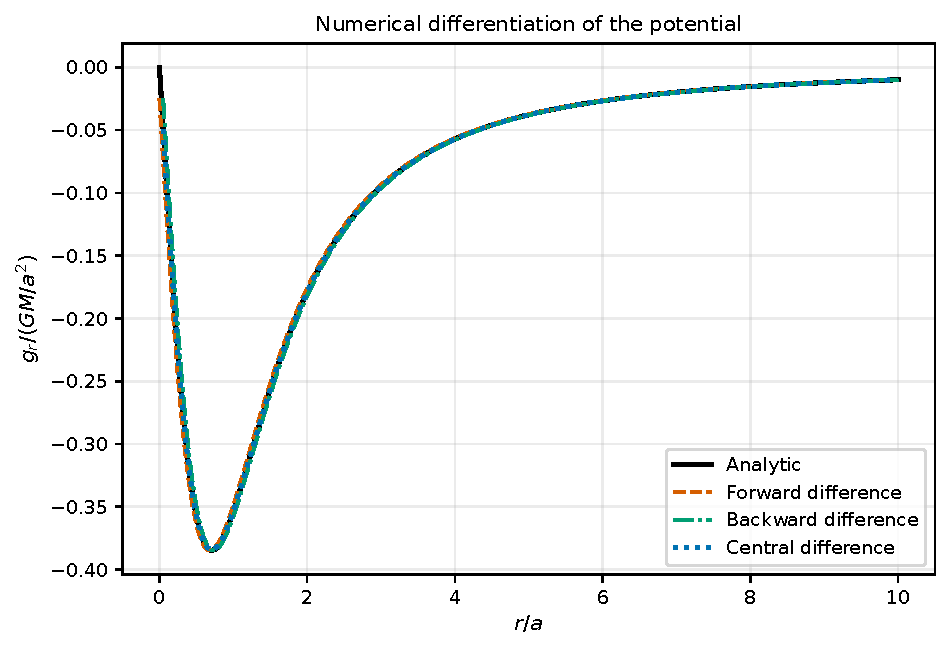
\includegraphics[width=0.68\linewidth]{ch02_differentiation.pdf}
\caption{$N=200$、$r_{\max}=10a$ の格子上で、解析的な Plummer ポテンシャルを前進・後退・中心差分して得た重力加速度。}
\label{fig:ch2-differentiation}
\end{figure}

一つの格子で結果を比較するだけでは、格子を細かくしたときに誤差がどの速さで減少するかは分からない。
この点を次節の格子収束試験で調べる。

% =====================================================================

\section{前進・後退・中心差分の収束比較}
\label{sec:ch2-diff-convergence}

前節では、一つの格子上で解析ポテンシャルを数値微分し、3つの差分公式から得られる重力加速度を比較した。
本節では格子幅を変えて同じ計算を繰り返し、前進差分・後退差分の1次収束と中心差分の2次収束を数値的に確認する。

数値微分そのものの収束性を調べるため、前節と同じく解析ポテンシャル $\Phi_{\rm exact}$ を入力として用いる。
計算領域を $r_{\max}=10a$ に固定し、区間数を
\begin{equation}
 N=50,100,200,400,800
\end{equation}
と変えて、5種類の格子で誤差を測る。

格子を変えると、各差分公式が重力加速度を返す格子点の位置も変わる。
そこで、すべての格子で同じ物理的な半径範囲を比較するため、
\begin{equation}
 0.2a\le r\le5a
\label{eq:ch2-diff-range}
\end{equation}
に含まれる評価点だけを用いる。
各差分公式について、規格化した最大絶対誤差を
\begin{equation}
 \epsilon_{g,\mathrm{fixed}}
 \equiv
 \max_{\substack{i\\0.2a\le r_i\le5a}}
 \frac{|g_{r,\mathrm{num}}(r_i)-g_{r,\mathrm{exact}}(r_i)|}{GM/a^2}
\label{eq:ch2-gravity-error-fixed}
\end{equation}
と定義する。
ここで $g_{r,\mathrm{num}}$ は各差分公式から得た重力加速度である。
分母の $GM/a^2$ は一定の基準量なので、
$\epsilon_{g,\mathrm{fixed}}$ は規格化した絶対誤差であり、
各点での相対誤差ではない。

\begin{notebookblock}{2｜数値微分の格子収束}
各格子について、解析ポテンシャルを3つの差分公式で微分し、
式\eqref{eq:ch2-gravity-error-fixed}の最大誤差を測る。
この処理を補助関数 \texttt{differentiation\_errors} にまとめる。

{\sffamily\small\color{graytext}対応セル（補助関数）}
\begin{Verbatim}[xleftmargin=2mm,fontsize=\small,frame=single,framesep=1.8mm,framerule=0.35pt,rulecolor=\color{listingframe},fillcolor=\color{listingbg}]
def differentiation_errors(N):
    r_max = 10.0 * a
    r = np.linspace(0.0, r_max, N + 1)
    dr = r[1] - r[0]
    phi = phi_plummer_exact(r, G, M, a)

    r_f, g_f = gravity_forward(r, phi)
    r_b, g_b = gravity_backward(r, phi)
    r_c, g_c = gravity_central(r, phi)

    def max_error(r_eval, g_num):
        mask = (r_eval >= 0.2 * a) & (r_eval <= 5.0 * a)
        g_exact = gravity_plummer_exact(r_eval, G, M, a)
        return np.max(np.abs(g_num[mask] - g_exact[mask])) / (G * M / a**2)

    return dr, max_error(r_f, g_f), max_error(r_b, g_b), max_error(r_c, g_c)
\end{Verbatim}

{\sffamily\small\color{graytext}対応セル（収束次数の測定）}
\begin{Verbatim}[xleftmargin=2mm,fontsize=\small,frame=single,framesep=1.8mm,framerule=0.35pt,rulecolor=\color{listingframe},fillcolor=\color{listingbg}]
# 5種類の格子で3手法の最大誤差を測る
N_diff = np.array([50, 100, 200, 400, 800])
results = np.array([differentiation_errors(int(N_i)) for N_i in N_diff])

dr_diff = results[:, 0]
err_forward = results[:, 1]
err_backward = results[:, 2]
err_central = results[:, 3]

# log(error)-log(dr) の傾きから収束次数を求める
order_forward = np.polyfit(np.log(dr_diff), np.log(err_forward), 1)[0]
order_backward = np.polyfit(np.log(dr_diff), np.log(err_backward), 1)[0]
order_central = np.polyfit(np.log(dr_diff), np.log(err_central), 1)[0]
\end{Verbatim}
\end{notebookblock}

5つの格子で得た誤差を両対数上で直線近似すると、
\begin{equation}
 p_{\rm f}=\chtwoForwardOrder,
 \qquad
 p_{\rm b}=\chtwoBackwardOrder,
 \qquad
 p_{\rm c}=\chtwoCentralOrder
\label{eq:ch2-diff-orders}
\end{equation}
を得る。添字 $\mathrm f,\mathrm b,\mathrm c$ は、それぞれ前進・後退・中心差分を表す。
図\ref{fig:ch2-differentiation-convergence}に示すように、
前進差分と後退差分はほぼ1次精度、中心差分はほぼ2次精度で収束しており、
前節で求めた各差分公式の誤差評価と一致する。
前進差分と後退差分の測定値が厳密に1にならないのは、
有限の格子幅では主要な1次誤差だけでなく、より高次の誤差項も寄与するためである。
格子をさらに細かくすると、それらの影響は小さくなり、
測定される収束次数は1に近づく。

\begin{figure}[!htbp]
\centering
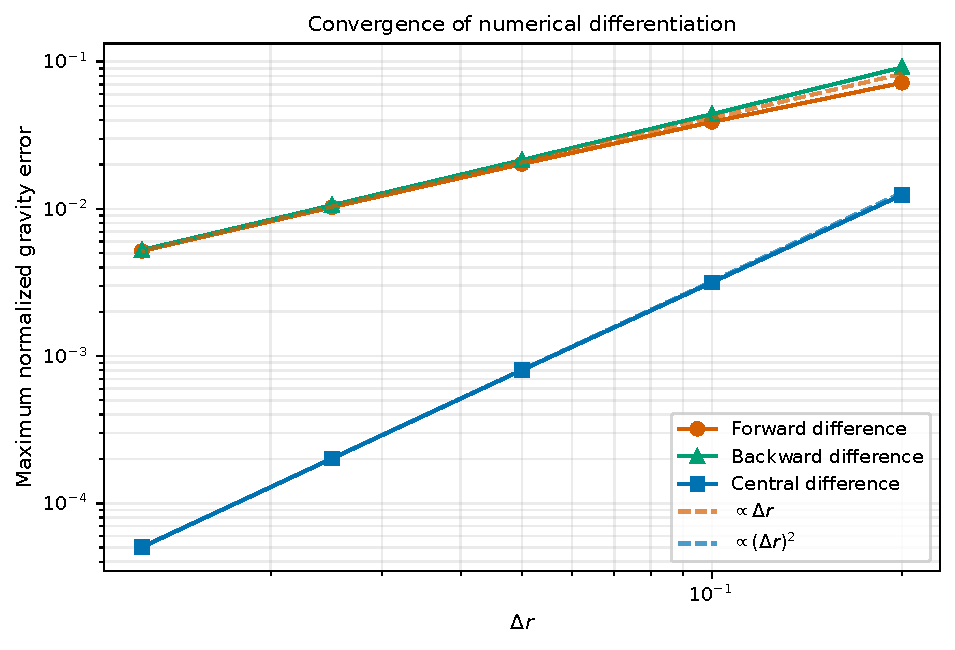
\includegraphics[width=0.68\linewidth]{ch02_differentiation_convergence.pdf}
\caption{解析的な Plummer ポテンシャルを数値微分したときの格子収束。$0.2a\le r\le5a$ で測った規格化最大絶対誤差を示す。前進・後退差分はほぼ1次、中心差分はほぼ2次で収束する。}
\label{fig:ch2-differentiation-convergence}
\end{figure}


以上で、密度分布から Poisson 方程式を解いてポテンシャルを求め、
その数値微分から重力加速度を計算するための手順がそろった。
ここまでの収束試験では、Poisson 方程式の求解と数値微分を分けて検証した。
Notebook 2 の「密度 $\rightarrow$ ポテンシャル $\rightarrow$ 重力」の計算例では、数値ポテンシャル $\Phi_{\rm num}$ を中心差分して
重力加速度を求め、解析解および第1章の累積台形則による内包質量から得た結果と比較する。

% =====================================================================
\begin{topicblock}{偏微分方程式の型と境界条件}
本章で扱った Poisson 方程式は、\textbf{楕円型（elliptic）}偏微分方程式の代表例である。
この境界値問題では、内部の方程式と境界条件を合わせ、領域全体で互いに結合した未知数を求める。
本章では中心と外側に条件を与え、有限差分で得た連立一次方程式を解いた。
付録\ref{app:linear-systems}の反復法を使う場合も、領域全体の方程式を満たす解へ近づける点は同じである。

熱伝導や拡散を記述する\textbf{放物型（parabolic）}と、波や移流を記述する\textbf{双曲型（hyperbolic）}の方程式も、宇宙流体計算で現れる。
有限領域でこれらの時間発展を求める問題は、初期条件と境界条件を組み合わせた\textbf{初期境界値問題（initial-boundary value problem）}として扱う。
正の拡散係数を持つ拡散方程式では、初期分布に加え、空間領域の境界全体で各時刻の条件を定める。
一方、双曲型では情報が有限の速さで伝わる経路を\textbf{特性曲線}と呼び、境界で与える独立な条件の数は、領域へ流入する特性の数で決まる。
例えば一定方向に進む移流では、流入側に値を与え、流出側の値は内部から伝わる解によって決まる。
この場合、流出側に独立な値を追加して固定してはいけない。
ただし、流出境界近くの数値更新に必要な値を、内部から外側へ延長する処理は必要になり得る。

本章では既知の境界値を右辺へ移したが、別の実装方法として、計算領域の外側に仮想的な値を置き、境界近傍でも内部と同じ形の更新式を使う方法がある。
格子法の流体計算で用いる\textbf{ゴーストセル（ghost cell）}はこの考え方に対応し、付録\ref{app:axisym-poisson}の対称軸の仮想点とも共通する。
例えば、周期境界では反対側の値をコピーし、反射境界では境界をはさんで対称な位置の値をコピーして、境界に垂直な速度成分の符号を反転する。
流出境界では内部の値を外挿する方法があるが、すべての波を無反射で通す保証はない。
必要な物理的条件と、その条件を実装する処理を分けて考えることが重要である。
境界条件とゴーストセルの扱いは、藤井・立川\cite{fujii2020}、松本ほか\cite{matsumoto}を参照すること。
\end{topicblock}

\begin{topicblock}{時間発展問題の時間積分と連立一次方程式}
時間発展を含む偏微分方程式でも、空間方向を有限差分などで離散化すると、各格子点の値についての連立常微分方程式が得られる。
これを時間方向へ進める方法には、陽的な方法と陰的な方法がある。

既知の状態と、すでに計算した途中の状態から、順に更新量を求める方法を\textbf{陽的な時間積分（explicit time integration）}という。
第3章で扱う Euler 法と陽的 Runge--Kutta 法では、時間更新の未知量について連立方程式を解く必要はない。
一方、空間離散化と組み合わせた時間刻みの制約を満たす必要がある。
例えば、一次元の圧縮性流体で全セルに共通の時間刻みを使う場合には、
\[
 \Delta t\le C_{\rm CFL}\min_i\frac{\Delta x_i}{|v_i|+c_{{\rm s},i}}
\]
という\textbf{CFL 条件（Courant--Friedrichs--Lewy condition）}が重要になる。
$\Delta x_i$ はセル幅、$v_i$ は流速、$c_{{\rm s},i}$ は音速であり、最も厳しいセルの条件を使う。
$C_{\rm CFL}$ の許容値は数値手法に依存し、この条件を満たすだけで任意の空間離散化が安定になるわけではない。
一定の拡散係数を持つ拡散方程式の陽解法では、許される時間刻みの上限は典型的に $\Delta t_{\max}\propto(\Delta x)^2$ となる。
高次精度の公式を選ぶことと、安定に時間発展を計算することは別である。

次の時刻や計算途中の未知の値を含む式を立て、その式を解いて更新する方法を\textbf{陰的な時間積分（implicit time integration）}という。
線形な問題では連立一次方程式に帰着するが、非線形な問題では非線形方程式を解く必要がある。
例として、本章の $u=r\Phi$ とは区別して拡散する量を $w(x,t)$ と書き、一定の拡散係数 $D>0$ を持つ方程式
\[
 \frac{\partial w}{\partial t}=D\frac{\partial^2 w}{\partial x^2}
\]
を考える。
一様格子上の値を $w_i^n\simeq w(x_i,t_n)$ とし、二階微分を中心差分、時間方向を後退 Euler 法で離散化すると、
\[
 \frac{w_i^{n+1}-w_i^n}{\Delta t}
 =D\frac{w_{i+1}^{n+1}-2w_i^{n+1}+w_{i-1}^{n+1}}{(\Delta x)^2}
\]
である。
これを整理すると、
\[
 -\alpha w_{i-1}^{n+1}+(1+2\alpha)w_i^{n+1}-\alpha w_{i+1}^{n+1}=w_i^n,
 \qquad \alpha=\frac{D\Delta t}{(\Delta x)^2}
\]
となる。
境界値を指定すれば、本章と同じ三重対角構造の連立一次方程式を各ステップで解くことになる。
この線形拡散問題に対する後退 Euler 法では、陽解法の拡散安定条件を避けられるが、大きな時間刻みでも時間変化を正確に追えるという意味ではない。
安定性による制約と、精度のために必要な時間刻みを区別する。

宇宙流体計算では、流体部分を陽的に進め、熱伝導や輻射の拡散など、時間刻みの制約が厳しい過程を陰的に扱うことがある。
また、流体の時間更新が陽的でも、自己重力を求めるには Poisson 方程式を解く。
本章では密度を固定したが、自己重力流体では密度分布が変わるため、時間積分の各段階と整合する密度から重力場を更新する必要がある。
詳しい解法は藤井・立川\cite{fujii2020}、松本ほか\cite{matsumoto}、自己重力との組合せは富阪ほか編\cite{tomisaka2007}を参照すること。
\end{topicblock}


\chapter{球対称ポテンシャルと時間積分法}
\label{chap:orbits}

第1--2章では、球対称な密度分布から重力場を求めた。
本章では、同じ Plummer 球の重力場の中で星の位置と速度の時間変化を計算し、常微分方程式の時間積分法を学ぶ。
時間積分そのものの誤差を調べるため、加速度には解析式を用い、第2章の数値重力場に含まれる誤差とは切り分けて検証する。

運動方程式に初期位置と初期速度を与えると、その後の軌道を求める初期値問題となる。
Euler 法、古典的4次 Runge--Kutta 法（RK4）、リープフロッグ法（leapfrog method）を同じ軌道に適用し、時間刻みを変えた収束試験と保存量の変化から結果を検証する。
軌道の物理は Ryden §7.1\cite{ryden2025}、Euler 法と RK4 は幸谷 第13章\cite{kouya2021}、リープフロッグ法の長時間挙動は松本ほか §9.6\cite{matsumoto}を参照する。

\begin{learningbox}[本章で学ぶこと]
\begin{itemize}
 \item 運動方程式を、位置と速度を未知数とする1階の常微分方程式系に書き換え、初期値問題として設定できる。
 \item Euler 法、RK4、リープフロッグ法の更新の考え方を説明し、時間ループとして実装できる。
 \item 円軌道の解析解との比較と時間刻みを変えた収束試験から、時間積分法の誤差と収束次数を評価できる。
 \item エネルギーと角運動量の変化を用いて数値軌道を診断し、保存量だけでは位置の精度を判断できないことを説明できる。
 \item 収束次数と長時間積分での保存量の振る舞いを区別し、必要な精度・積分時間・計算コストに応じて時間積分法を選ぶ際の考え方を説明できる。
\end{itemize}
\end{learningbox}

本章の数値実験は Notebook 3 で行う。
本文では更新式と計算部分の対応を示し、完全な可視化コードは Notebook に置く。
軸対称・非軸対称の軌道は付録\ref{app:orbit-applications}で扱い、本章は球対称モデルだけで学習できる。
% =====================================================================
\section{Plummer 球の重力場と軌道計算の準備}
\label{sec:ch3-plummer}

第1--2章で用いた Plummer ポテンシャル
\begin{equation}
 \Phi(r)=-\frac{GM}{\sqrt{r^2+a^2}}
\label{eq:ch3-plummer-potential}
\end{equation}
の中で星の軌道を計算する。
重力場は時間に依存せず、計算する星の運動によっても変化しないものとする。
中心から測った位置ベクトルを $\boldsymbol{x}$、その大きさを $r=|\boldsymbol{x}|$ と書く。
第2章と同様に、動径方向の重力加速度を $g_r=-d\Phi/dr$ とする。
軌道計算では重力加速度をベクトルとして扱うため、以下では重力加速度ベクトルを $\boldsymbol{g}$ と書く。
球対称系では、中心以外で
\begin{equation}
 \boxed{\boldsymbol{g}=g_r\frac{\boldsymbol{x}}{r}=-\frac{GM}{(r^2+a^2)^{3/2}}\boldsymbol{x}}
\label{eq:ch3-plummer-acc}
\end{equation}
となる。この右辺は中心でもそのまま評価でき、$\boldsymbol{g}(\boldsymbol{0})=\boldsymbol{0}$ である。\footnote{
このポテンシャルは、無衝突系を扱う重力 $N$ 体計算で用いられる\textbf{Plummer 型ソフトニング（softening）}と同じ関数形を持つ\cite{matsumoto}。
粒子間距離を $r$、粒子質量を $m$ とし、ポテンシャルを $-Gm/\sqrt{r^2+\epsilon^2}$ とすると、$\epsilon>0$ なら $r\to0$ でも重力加速度は発散しない。
ただし、本章の $a$ は質量モデル全体のスケール半径であり、$\epsilon$ は粒子間の重力を平滑化する長さである。
同じ関数形に現れるが、両者の役割は異なる。
}

Notebook 3 では $G=M=a=1$ の無次元単位を用いる。
質量単位を $M$、長さ単位を $a$ とし、時間単位 $t_\ast$ を $a/t_\ast^2=GM/a^2$ となるように選ぶと、
\begin{equation}
 t_\ast=\sqrt{\frac{a^3}{GM}},\qquad
 v_\ast=\sqrt{\frac{GM}{a}},\qquad
 \Phi_\ast=\frac{GM}{a}
\label{eq:ch3-dynamical-units}
\end{equation}
を得る。
無次元の時刻・速度・ポテンシャルを物理単位へ戻すときは、それぞれ $t_\ast$、$v_\ast$、$\Phi_\ast$ を掛ければよい。

以下では、位置ベクトルから Plummer ポテンシャルと重力加速度を
計算する関数を定義する。

\begin{notebookblock}{3｜Plummer 球の重力場}
初期条件・解析解・軌道計算で同じ $G,M,a$ を使う。

\texttt{phi\_plummer\_pos} は、位置ベクトルからポテンシャルを計算する。
\texttt{np.sum(x**2, axis=-1)} は、位置ベクトルの各成分の二乗和を求める。
\texttt{axis=-1} は配列の最後の軸を指定しており、
複数の時刻の位置をまとめて与えた場合にも、それぞれのポテンシャルを計算できる。

\texttt{acc\_plummer} は、一つの位置ベクトルから重力加速度を計算する。
\texttt{acc\_plummer\_model} は、設定した $G,M,a$ を用いて、
位置ベクトルだけから加速度を計算する補助関数である。
後の時間積分では、この関数を使用する。

\par\smallskip\noindent\begin{minipage}{\linewidth}
{\sffamily\small\color{graytext}対応セル（重力場の定義）}
\begin{Verbatim}[xleftmargin=2mm,fontsize=\small,frame=single,framesep=1.8mm,framerule=0.35pt,rulecolor=\color{listingframe},fillcolor=\color{listingbg}]
import numpy as np

# 無次元単位を設定する
G = 1.0
M = 1.0
a = 1.0

# 位置ベクトルからPlummerポテンシャルを計算する
def phi_plummer_pos(x, G, M, a):
    x = np.asarray(x)
    r2 = np.sum(x**2, axis=-1)
    return -G * M / np.sqrt(r2 + a**2)

# 一つの位置ベクトルから加速度を計算する
def acc_plummer(x, G, M, a):
    x = np.asarray(x)
    r2 = np.dot(x, x)
    return -G * M * x / (r2 + a**2)**1.5

# 時間積分で用いる加速度関数
def acc_plummer_model(x):
    return acc_plummer(x, G, M, a)
\end{Verbatim}
\end{minipage}

\end{notebookblock}

球対称ポテンシャル中では角運動量が保存されるため、恒星の軌道は一つの平面内に限られる。
そこで、本章では $x$--$y$ 平面内の軌道を扱う。

% =====================================================================
\section{初期値問題としての運動方程式}
\label{sec:ch3-ode}

軌道を計算するには、前節の加速度を使って位置と速度の変化を求める。
位置を $\boldsymbol{x}$、速度を $\boldsymbol{v}$ とすると、運動方程式は
\begin{equation}
 \frac{d\boldsymbol{x}}{dt}=\boldsymbol{v},\qquad
 \frac{d\boldsymbol{v}}{dt}=-\nabla\Phi(\boldsymbol{x})\equiv\boldsymbol{g}(\boldsymbol{x})
\label{eq:ch3-eom}
\end{equation}
である。
位置と速度を一つの\textbf{状態ベクトル}にまとめ、
\begin{equation}
 \boldsymbol{y}=\begin{pmatrix}\boldsymbol{x}\\\boldsymbol{v}\end{pmatrix}
\label{eq:ch3-state}
\end{equation}
と書くと、
\begin{equation}
 \frac{d\boldsymbol{y}}{dt}=\boldsymbol{f}(\boldsymbol{y})
\label{eq:ch3-first-order}
\end{equation}
という1階の常微分方程式（ordinary differential equation; ODE）の連立系になる。
右辺は、現在の位置と速度からその変化率を返す関数であり、
\begin{equation}
 \boldsymbol{f}(\boldsymbol{y})=\begin{pmatrix}\boldsymbol{v}\\\boldsymbol{g}(\boldsymbol{x})\end{pmatrix}
\label{eq:ch3-rhs}
\end{equation}
である。
本章の重力場は時間に依存しないため、右辺には時刻 $t$ が明示的には現れない。
この形にすれば、一般の常微分方程式の時間積分法を軌道計算に適用できる\footnote{
自己重力の $N$ 体計算では、各粒子の加速度を全粒子の配置から求めるため、粒子の運動に伴って重力場も変化する。
全粒子の位置と速度をまとめれば同じ常微分方程式系の形で書けるが、粒子同士の運動は結びついており、各粒子を独立した固定場中の軌道として積分するわけではない\cite{tomisaka2007}。
}

運動方程式だけでは、星がどの軌道をたどるかは決まらない。
本章では、初期時刻 $t=0$ における位置 $\boldsymbol{x}(0)=\boldsymbol{x}_0$ と速度 $\boldsymbol{v}(0)=\boldsymbol{v}_0$ を与え、その後の状態を求める。
第2章で空間の両端に条件を与えた境界値問題とは、条件を与える場所と解の求め方が異なる。

\begin{definitionbox}{初期値問題}
微分方程式と、初期時刻に与える条件を組み合わせてその後の解を求める問題を、\textbf{初期値問題（initial-value problem）}と呼ぶ。
\end{definitionbox}

数値計算では、一定の時間刻み $\Delta t$ を用い、
\begin{equation}
 t_n=n\Delta t,\qquad n=0,1,2,\ldots
\label{eq:ch3-time-grid}
\end{equation}
という離散的な時刻で状態を求める。
時刻 $t_n$ の厳密な状態を $\boldsymbol{y}(t_n)$、その数値近似を $\boldsymbol{y}_n$ と書く。
以下の時間積分法では、既知の $\boldsymbol{y}_n$ から次の時刻の $\boldsymbol{y}_{n+1}$ を求める操作を繰り返す。
% =====================================================================
\section{Euler 法}
\label{sec:ch3-euler}

最も基本的な時間積分法が Euler 法（Euler method）である。
現在の状態の変化率を、次の時刻まで一定とみなして解を進める。
この更新式は、時刻 $t_n$ の厳密解を Taylor 展開すると理解できる。
\begin{equation}
 \boldsymbol{y}(t_n+\Delta t)=\boldsymbol{y}(t_n)
 +\Delta t\left.\frac{d\boldsymbol{y}}{dt}\right|_{t_n}
 +\frac{\Delta t^2}{2}\left.\frac{d^2\boldsymbol{y}}{dt^2}\right|_{t_n}
 +O(\Delta t^3).
\label{eq:ch3-euler-taylor}
\end{equation}
式\eqref{eq:ch3-first-order}を使い、$\Delta t^2$ 以上の項を省略して数値近似を更新すると、
\begin{equation}
 \boxed{\boldsymbol{y}_{n+1}=\boldsymbol{y}_n+\Delta t\,\boldsymbol{f}(\boldsymbol{y}_n)}
\label{eq:ch3-euler}
\end{equation}
を得る。


この更新の意味を、1変数の方程式 $dy/dt=f(y)$ で考える。
$t$--$y$ 平面では、始点での変化率 $k_1=f(y_n)$ は、その点での傾きに対応する。
Euler 法は、この傾きを保つ直線に沿って時間幅 $\Delta t$ だけ進み、$y_{n+1}=y_n+\Delta t\,k_1$ と更新する。
図\ref{fig:ch3-euler-geometry}では、時間とともに増加する解を持つ $dy/dt=1+y^2$ を例に、$t_n=0$、$y_n=0$、$\Delta t=1$ の1ステップを示す。
この初期条件に対する厳密解は $y(t)=\tan t$ である。
始点の傾きは $k_1=1$ なので、Euler 法の次の値は $y_{n+1}=1$ となるが、厳密解は $y(1)=\tan 1\simeq1.5574$ である。
%この図は星の軌道の形ではなく、説明用の変数 $y$ の時間変化を表している。

\begin{figure}[!htbp]
\centering
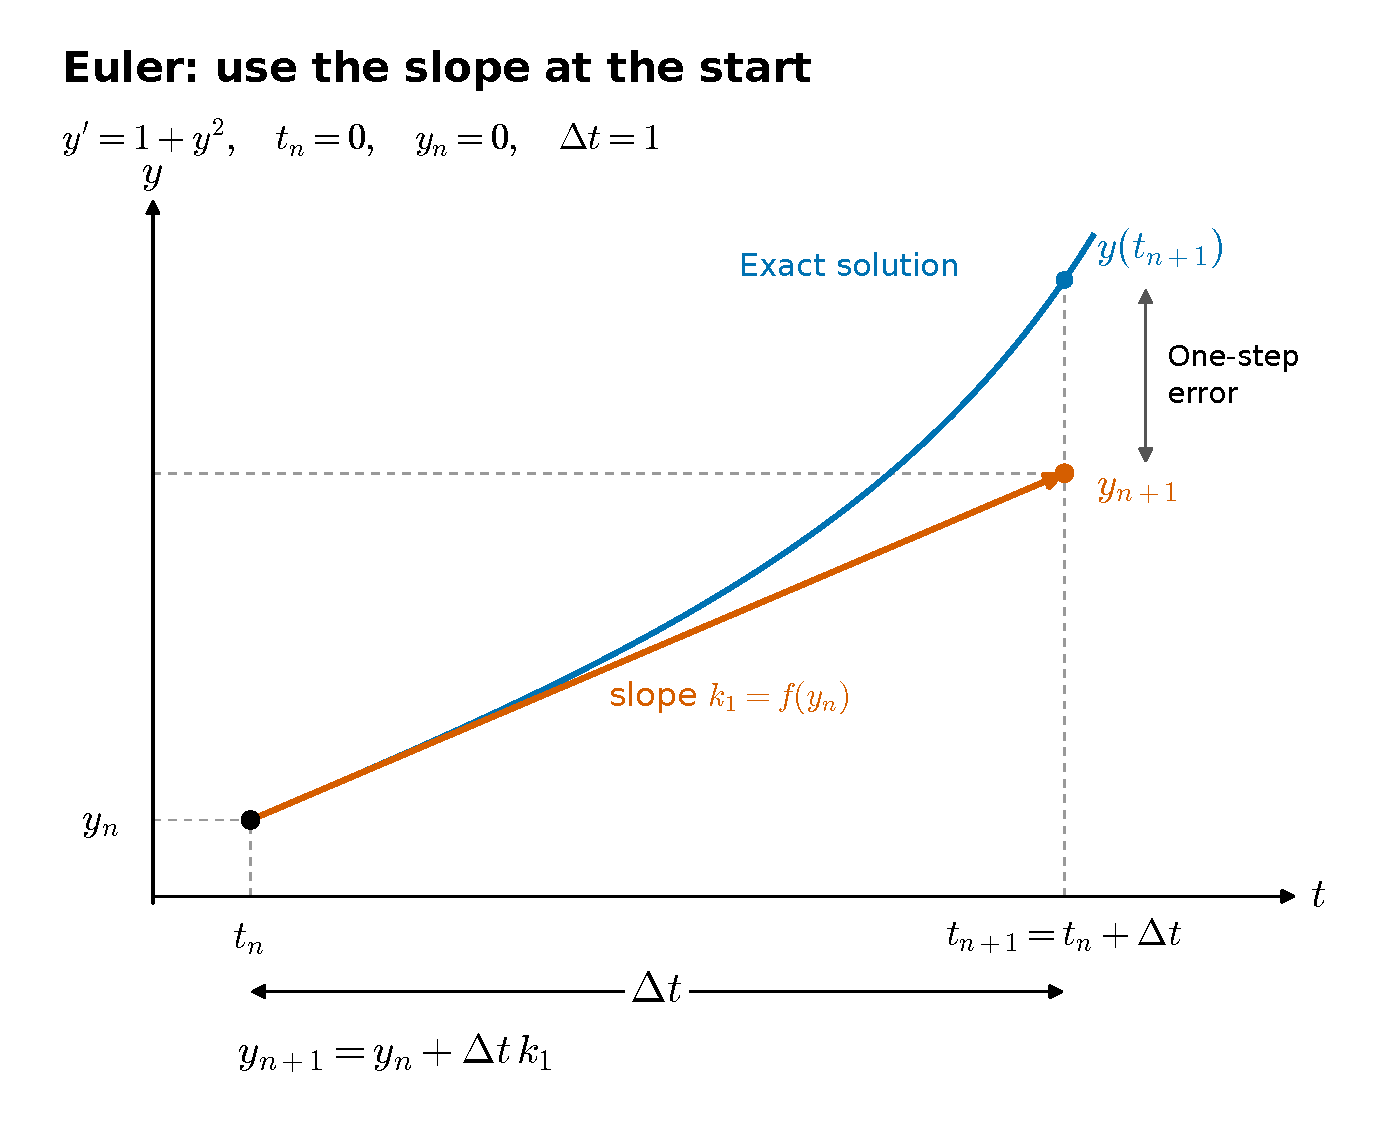
\includegraphics[width=0.60\linewidth]{ch03_euler_geometry.pdf}
\caption{Euler 法の1ステップ。青い曲線は厳密解 $y(t)=\tan t$、朱色の直線は始点の傾き $k_1=f(y_n)$ を用いた更新を表す。下の横矢印は時間幅 $\Delta t$、右の縦矢印は同じ終端時刻における厳密解と数値近似の差を示す。始点を厳密に与えているため、この差の大きさが1ステップの局所打ち切り誤差の大きさに対応する。}
\label{fig:ch3-euler-geometry}
\end{figure}

時刻 $t_n$ の値が厳密であるとして、1ステップで生じるずれを\textbf{局所打ち切り誤差}と呼ぶ。
Euler 法では、省略した最初の項から、この誤差は $O(\Delta t^2)$ である。
一方、更新を繰り返して得られる数値解には、それまでの局所的な誤差が伝播・累積した\textbf{大域誤差}が含まれる。
滑らかな右辺に対して十分小さい時間刻みを用い、固定した終端時刻まで積分すると、Euler 法の大域誤差は $O(\Delta t)$ となり、1次精度である\cite{kouya2021}。
この収束次数は §\ref{sec:ch3-convergence}で数値的に測定する。

式\eqref{eq:ch3-euler}を位置と速度へ書き戻すと、
\begin{align}
 \boldsymbol{x}_{n+1}&=\boldsymbol{x}_n+\Delta t\,\boldsymbol{v}_n,\label{eq:ch3-euler-x}\\
 \boldsymbol{v}_{n+1}&=\boldsymbol{v}_n+\Delta t\,\boldsymbol{g}(\boldsymbol{x}_n).\label{eq:ch3-euler-v}
\end{align}
これらの更新式を Python に対応させたものが Listing 3.1 である。
\begin{listingbox}{3.1　Euler 法の1ステップ}
\begin{Verbatim}[fontsize=\small]
# 位置と速度の両方を、更新前の値から求める
x_new = x + dt * v
v_new = v + dt * acc_func(x)
\end{Verbatim}
\end{listingbox}
ここで、\texttt{acc\_func} は、位置を受け取って加速度を返す関数を表す引数である。
Plummer 球の軌道計算では、前節で定義した\texttt{acc\_plummer\_model} を指定する。
このように加速度関数を指定することで、同じ時間積分法を異なる重力ポテンシャルにも適用できる。
また、\texttt{dt} は時間刻み $\Delta t$ を表す。

Euler 法では、位置と速度の両方を時刻 $t_n$ の値から計算する。
したがって、速度の更新に用いる加速度は、更新後の位置 \texttt{x\_new} ではなく、
更新前の位置 \texttt{x} から求める。
この1ステップの処理を時間ループで繰り返す実装は、§\ref{sec:ch3-circular-test}で示す。

% =====================================================================
\section{古典的4次 Runge--Kutta 法（RK4）}
\label{sec:ch3-rk4}

Euler 法は、1ステップの始点での変化率だけを使う。
Runge--Kutta 法では、時間区間内の状態を予測して右辺を複数回評価し、その結果を組み合わせて高い精度を得る。
古典的4次 Runge--Kutta 法（RK4）では、次の4つの変化率を計算する。
\begin{align}
 \boldsymbol{k}_1&=\boldsymbol{f}(\boldsymbol{y}_n),\label{eq:ch3-rk-k1}\\
 \boldsymbol{k}_2&=\boldsymbol{f}\left(\boldsymbol{y}_n+\frac{\Delta t}{2}\boldsymbol{k}_1\right),\label{eq:ch3-rk-k2}\\
 \boldsymbol{k}_3&=\boldsymbol{f}\left(\boldsymbol{y}_n+\frac{\Delta t}{2}\boldsymbol{k}_2\right),\label{eq:ch3-rk-k3}\\
 \boldsymbol{k}_4&=\boldsymbol{f}\left(\boldsymbol{y}_n+\Delta t\,\boldsymbol{k}_3\right).\label{eq:ch3-rk-k4}
\end{align}
$\boldsymbol{k}_1$ は始点での変化率、$\boldsymbol{k}_2$ と $\boldsymbol{k}_3$ は中間時刻、$\boldsymbol{k}_4$ は終点時刻の予測状態での変化率である。
$\boldsymbol{k}_2$ と $\boldsymbol{k}_3$ は同じ中間時刻に対応するが、その評価に用いる状態の予測値が異なる。
これらを使って、
\begin{equation}
 \boxed{\boldsymbol{y}_{n+1}=\boldsymbol{y}_n+\frac{\Delta t}{6}
 \left(\boldsymbol{k}_1+2\boldsymbol{k}_2+2\boldsymbol{k}_3+\boldsymbol{k}_4\right)}
\label{eq:ch3-rk4}
\end{equation}
と更新する\cite{kouya2021}。

\subsection{RK4の幾何学的説明}
図\ref{fig:ch3-rk4-geometry}では、図\ref{fig:ch3-euler-geometry}と同じ $dy/dt=1+y^2$ の例を使い、4つの傾きと最終更新を一つの $t$--$y$ 平面に示す。
図中の $Y_2,Y_3,Y_4$ は、それぞれ $k_2,k_3,k_4$ を評価するための予測値であり、
\begin{equation*}
 Y_2=y_n+\frac{\Delta t}{2}k_1,\qquad
 Y_3=y_n+\frac{\Delta t}{2}k_2,\qquad
 Y_4=y_n+\Delta t\,k_3
\end{equation*}
と書ける。
いずれも元の $y_n$ を基準に作る値であり、$Y_2$ と $Y_3$ は同じ中間時刻 $t_n+\Delta t/2$ に対する異なる予測である。
これらは厳密解の曲線上にあるとは限らない。

4つの傾きがそろったら、重み付き平均 $\bar{k}=(k_1+2k_2+2k_3+k_4)/6$ を求め、始点から $y_{n+1}=y_n+\Delta t\,\bar{k}$ と更新する。
この例では、$Y_4\simeq1.3906$ に対して最終値は $y_{n+1}\simeq1.5358$ となり、厳密解 $y(1)\simeq1.5574$ に近い。
最後の予測値 $Y_4$ をそのまま採用するのではなく、4つの傾きを組み合わせて次の値を決める点が重要である。

\begin{figure}[!htbp]
\centering
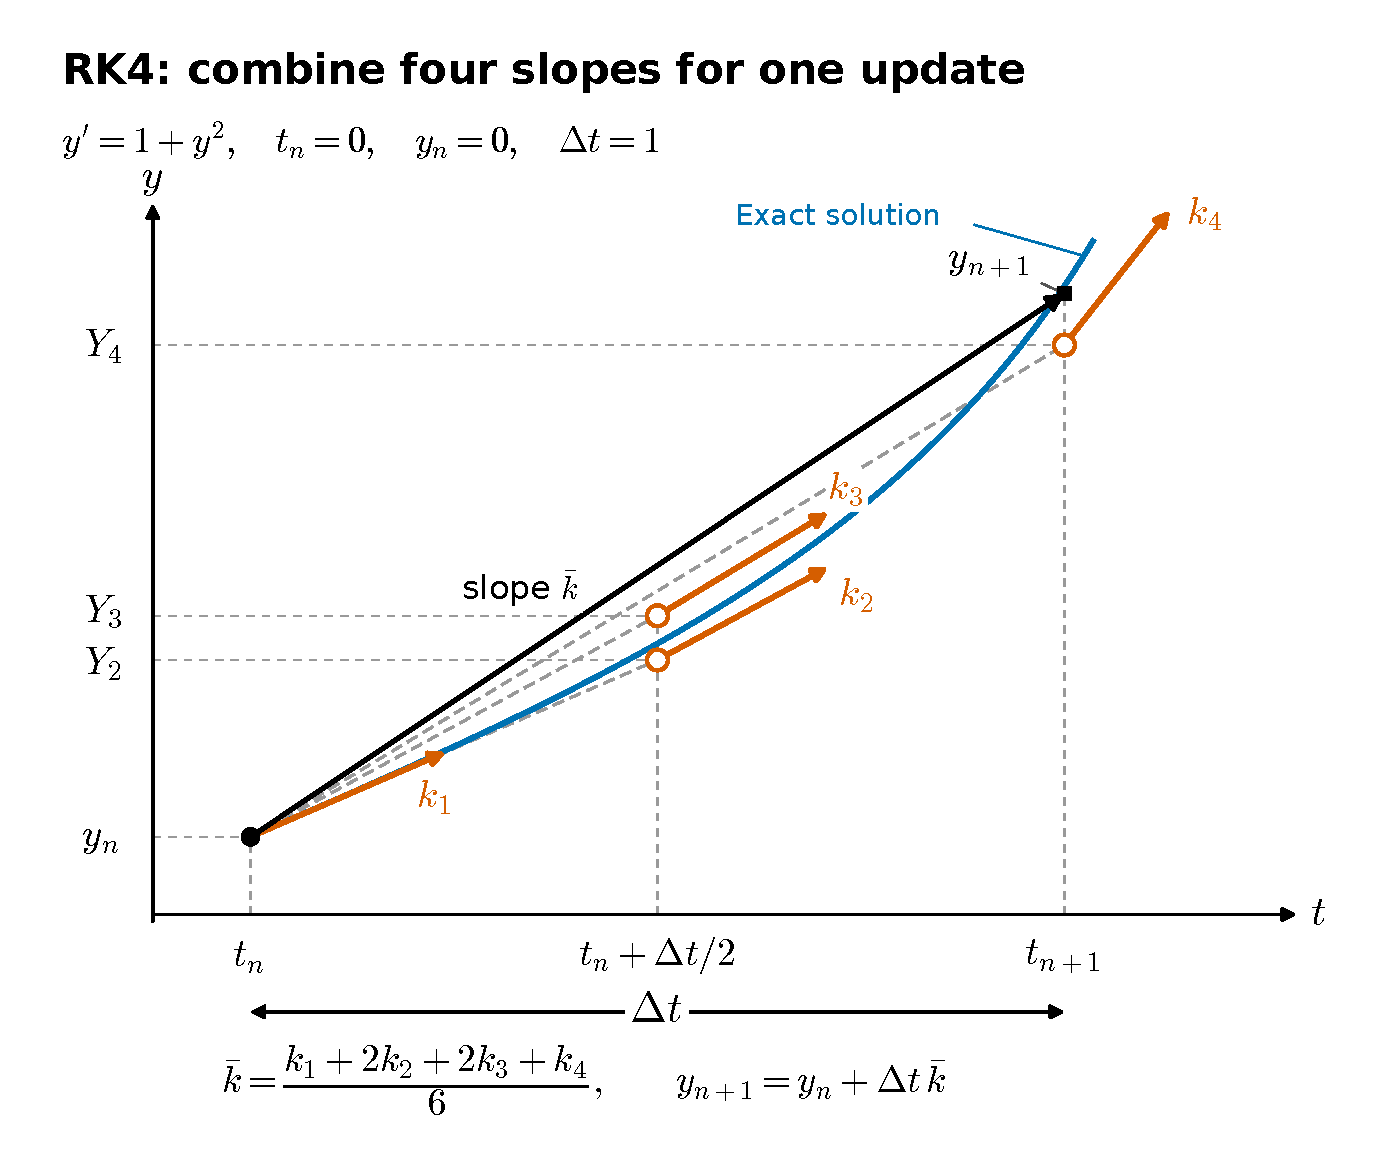
\includegraphics[width=0.60\linewidth]{ch03_rk4_geometry.pdf}
\caption{RK4 の4つの傾きと1ステップの更新。青い曲線は厳密解、白丸は予測値 $Y_2,Y_3,Y_4$、朱色の短い矢印は各評価点での傾き $k_1,k_2,k_3,k_4$ を表す。灰色の斜めの破線は始点から予測値を作る操作を示す。黒い矢印は平均傾き $\bar{k}$ を用いた最終更新であり、その終点の黒四角が $y_{n+1}$ である。この矢印や予測値を結ぶ線は、ステップ途中の解の曲線を表すものではない。}
\label{fig:ch3-rk4-geometry}
\end{figure}

中間状態の作り方と重み $1:2:2:1$ の組み合わせにより、厳密解の Taylor 展開と $\Delta t$ の4次まで一致する。
滑らかな右辺に対し、1ステップの局所打ち切り誤差は $O(\Delta t^5)$ である。
十分小さい時間刻みで固定した終端時刻まで積分したときの大域誤差は $O(\Delta t^4)$ となり、4次精度である。
ここでは更新式の使い方を学び、次数は円軌道の収束試験でも確かめる。

Notebook では、状態ベクトルを位置と速度の順に連結した1本の配列として扱う。
\texttt{ndim} は空間の次元数で、本章の平面内の運動では2である。
また、\texttt{y[n]} は時刻 $t_n$ の状態ベクトルを表す。

Listing 3.2 に、RK4 法の1ステップの計算を示す。
\begin{listingbox}{3.2　古典的4次 Runge--Kutta 法の1ステップ}
\begin{Verbatim}[fontsize=\small]
# 状態ベクトルから位置と速度を取り出し、時間微分を計算する
def rhs(state):
    x = state[:ndim]
    v = state[ndim:]
    return np.concatenate([v, acc_func(x)])

# 4つの予測状態で変化率を求め、次の状態を計算する
yn = y[n]
k1 = rhs(yn)
k2 = rhs(yn + 0.5 * dt * k1)
k3 = rhs(yn + 0.5 * dt * k2)
k4 = rhs(yn + dt * k3)
y[n + 1] = yn + dt * (k1 + 2*k2 + 2*k3 + k4) / 6.0
\end{Verbatim}
\end{listingbox}
ここで、\texttt{rhs} は式\eqref{eq:ch3-rhs}に対応し、状態ベクトルからその時間微分を計算する関数である。
\texttt{state[:ndim]} と \texttt{state[ndim:]} は、状態ベクトルから位置と速度をそれぞれ取り出す。
また、\texttt{np.concatenate} は複数の配列を一つにつなぐ関数であり、
ここでは速度と加速度をまとめて、状態ベクトルの時間微分を作る。

RK4 法は Euler 法より高次精度であるが、1ステップで右辺を4回評価する。
積分法を選ぶ際には、必要な精度だけでなく、計算コストも考慮する必要がある。
例えば、$N_{\rm p}$ 個の粒子間の重力を直接計算する重力多体系では、
全粒子対の重力を評価するため、1回の加速度計算に
$O(N_{\rm p}^2)$ の計算量がかかる\cite{tomisaka2007}。
このような計算では、時間積分法が必要とする加速度の評価回数も重要になる。

% =====================================================================
\section{リープフロッグ法（蛙跳び法）}
\label{sec:ch3-leapfrog}

本章のように加速度が位置だけで決まる場合には、
運動方程式を
\begin{equation}
 \ddot{\boldsymbol{x}}=\boldsymbol{g}(\boldsymbol{x})
\label{eq:ch3-second-order}
\end{equation}
と書ける。ドットは時間に関する微分を表す。
この式は、位置と速度に関する2つの一階微分方程式
\begin{align}
 \dot{\boldsymbol{x}}&=\boldsymbol{v},\\
 \dot{\boldsymbol{v}}&=\boldsymbol{g}(\boldsymbol{x})
\end{align}
に分けられる。

ここで、速度の変化率は位置だけで決まり、位置の変化率は速度だけで決まることに注目する。
この性質を利用すると、時間積分を2つの簡単な操作に分けて考えられる。
一つは、位置を固定して速度だけを更新する操作であり、キック（kick）と呼ぶ。
もう一つは、速度を固定して位置だけを更新する操作であり、ドリフト（drift）と呼ぶ。
リープフロッグ法は、この2つの操作を組み合わせて時間積分を行う方法である。

キックとドリフトを組み合わせる方法には、
キック--ドリフト--キック（kick--drift--kick; KDK）形式と、
ドリフト--キック--ドリフト（drift--kick--drift; DKD）形式がある。
どちらも2次精度のリープフロッグ法である。
本章ではKDK形式を用いる。この方法では、位置の更新（ドリフト）を
2つの半ステップの速度更新（キック）ではさむ。
この対称的な構成により、2次精度の時間積分法となる。

\subsection{KDKリープフロッグ法}
まず速度を半ステップ更新し、
\begin{equation}
 \boldsymbol{v}_{n+1/2}=\boldsymbol{v}_n+\frac{\Delta t}{2}\boldsymbol{g}(\boldsymbol{x}_n),
\label{eq:ch3-kick1}
\end{equation}
その補助速度で位置を1ステップ更新する。
\begin{equation}
 \boldsymbol{x}_{n+1}=\boldsymbol{x}_n+\Delta t\,\boldsymbol{v}_{n+1/2}.
\label{eq:ch3-drift}
\end{equation}
次に、新しい位置で加速度を評価し、速度を残り半ステップ更新する。
\begin{equation}
 \boldsymbol{v}_{n+1}=\boldsymbol{v}_{n+1/2}+\frac{\Delta t}{2}\boldsymbol{g}(\boldsymbol{x}_{n+1}).
\label{eq:ch3-kick2}
\end{equation}
すなわち、
\begin{equation}
 \boldsymbol{v}_n\rightarrow\boldsymbol{v}_{n+1/2}\rightarrow\boldsymbol{x}_{n+1}\rightarrow\boldsymbol{v}_{n+1}
\label{eq:ch3-leapfrog-flow}
\end{equation}
という計算順序で位置と速度を更新する。
ここで $\boldsymbol{v}_{n+1/2}$ は計算途中の補助速度であり、
この一連の操作で時刻 $t_n$ から $t_{n+1}=t_n+\Delta t$ まで進む。
一定の時間刻みでは、KDK形式で隣り合うステップの半ステップのキックをまとめると、
位置と速度を半ステップずれた時刻で交互に更新する形になる。
リープフロッグ（蛙跳び）という名前は、この互い違いの更新に由来する。
図\ref{fig:ch3-kdk}に、その時間的な配置を示す。
\begin{figure}[!htbp]
\centering
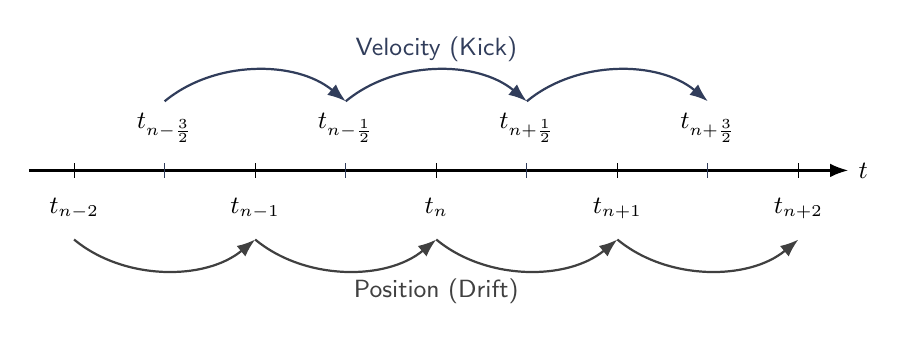
\begin{tikzpicture}[x=1.15cm,y=0.75cm,>=Latex,font=\sffamily\small]
% 時間軸：整数時刻に位置、半整数時刻に速度を配置
\draw[->,thick] (-0.5,0) -- (8.55,0) node[right] {$t$};
\foreach \i/\lab in {0/{n-2},2/{n-1},4/{n},6/{n+1},8/{n+2}}{
  \draw (\i,0.12) -- (\i,-0.12);
  \node[below=4pt] at (\i,-0.12) {$t_{\lab}$};
}
\foreach \i/\lab in {1/{n-\frac{3}{2}},3/{n-\frac{1}{2}},5/{n+\frac{1}{2}},7/{n+\frac{3}{2}}}{
  \draw[navy!85] (\i,0.12) -- (\i,-0.12);
  \node[above=4pt] at (\i,0.12) {$t_{\lab}$};
}
% 速度は位置の時刻を飛び越して更新する（Kick）
\foreach \i/\j in {1/3,3/5,5/7}{
  \draw[->,thick,navy!85] (\i,1.17)
    .. controls + (0.55,0.70) and +(-0.55,0.70) .. (\j,1.17);
}
% 位置は速度の時刻を飛び越して更新する（Drift）
\foreach \i/\j in {0/2,2/4,4/6,6/8}{
  \draw[->,thick,black!75] (\i,-1.17)
    .. controls + (0.55,-0.70) and +(-0.55,-0.70) .. (\j,-1.17);
}
\node[text=navy!85] at (4,2.05) {Velocity (Kick)};
\node[text=black!75] at (4,-2.05) {Position (Drift)};
\end{tikzpicture}
\caption{リープフロッグ法における位置と速度の時間的な配置。
位置は整数時刻、速度は半整数時刻に対応する。
上側の矢印は速度の更新（kick）、下側の矢印は位置の更新（drift）を表す。
位置と速度が半ステップずれて交互に更新されることが、「蛙跳び」という名前の由来である。}
\label{fig:ch3-kdk}
\end{figure}

式\eqref{eq:ch3-kick1}--\eqref{eq:ch3-kick2}は、Listing 3.3 の3行に対応する。

\begin{listingbox}{3.3　リープフロッグ法の1ステップ}
\begin{Verbatim}[fontsize=\small]
# 速度を半ステップ、位置を1ステップ、速度を半ステップ更新する
v_half = v + 0.5 * dt * acc_func(x)
x_new = x + dt * v_half
v_new = v_half + 0.5 * dt * acc_func(x_new)
\end{Verbatim}
\end{listingbox}

リープフロッグ法は、滑らかな加速度に対して2次精度の時間積分法である。
その収束次数は §\ref{sec:ch3-convergence}の数値実験で確認する。
更新式から誤差次数を求める計算は、以下の補足に示す。

Listing 3.3 では、各ステップの最初と最後に加速度を計算している。
しかし、前のステップの最後に求めた加速度は、
次のステップの最初にも使えるため、保存して再利用すれば計算回数を減らせる。
本書では、更新式との対応を分かりやすくするため、加速度を毎回計算している。

\begin{topicblock}{リープフロッグ法が2次精度になる理由}
時刻 $t_n$ の位置と速度が厳密であるとして、1ステップの誤差を調べる。
最初の速度更新を位置更新へ代入すると、
\begin{equation}
 \boldsymbol{x}_{n+1}=\boldsymbol{x}_n+\Delta t\,\boldsymbol{v}_n+\frac{\Delta t^2}{2}\boldsymbol{g}(\boldsymbol{x}_n)
\label{eq:ch3-leapfrog-position-combined}
\end{equation}
となる。これは位置の Taylor 展開を2次まで残した式である。
滑らかな加速度なら、厳密解の次項は $\Delta t^3\dot{\boldsymbol{g}}_n/6$ である。
ここで $\dot{\boldsymbol{g}}_n$ は、軌道に沿った加速度の時間微分を $t_n$ で評価した値を表す。
したがって、位置の局所打ち切り誤差は $O(\Delta t^3)$ である。

2回の速度更新をまとめると、
\begin{equation}
 \boldsymbol{v}_{n+1}=\boldsymbol{v}_n+\frac{\Delta t}{2}
 \left[\boldsymbol{g}(\boldsymbol{x}_n)+\boldsymbol{g}(\boldsymbol{x}_{n+1})\right]
\label{eq:ch3-leapfrog-velocity-combined}
\end{equation}
となる。一方、厳密な速度変化は
\begin{equation}
 \boldsymbol{v}(t_{n+1})-\boldsymbol{v}(t_n)=\int_{t_n}^{t_{n+1}}\boldsymbol{g}(\boldsymbol{x}(t))\,dt
\end{equation}
である。
式\eqref{eq:ch3-leapfrog-velocity-combined}は、加速度の時間積分に第1章の台形則を適用した形になっている。
厳密な端点加速度を用いた場合、台形則による1区間の誤差は $O(\Delta t^3)$ である。

実際には、終点の加速度を数値的な位置 $\boldsymbol{x}_{n+1}$ で評価する。
この位置には $O(\Delta t^3)$ の誤差があるため、滑らかな加速度では、その評価値の誤差も $O(\Delta t^3)$ となる。
ただし、速度更新ではこれに $\Delta t/2$ を掛けるので、速度への寄与は $O(\Delta t^4)$ である。
この寄与は台形則の主要な誤差より高次であり、速度の局所打ち切り誤差は $O(\Delta t^3)$ のままである。

固定した終端時刻までのステップ数は $O(\Delta t^{-1})$ である。
滑らかな力に対して安定に積分できる範囲では、局所的な誤差の伝播・累積を含めた位置と速度の大域誤差は、ともに $O(\Delta t^2)$ となる。
これがリープフロッグ法の2次精度に対応する。
\end{topicblock}
% =====================================================================
\section{円軌道による時間積分法の検証}
\label{sec:ch3-circular-test}

ここまでに示した3つの更新式を繰り返して、実際に軌道を計算する。
まず位置の解析解が分かる円軌道を用い、同じ初期条件と時間刻みで得た結果を比較する。

\subsection{円軌道の解析解}

半径 $r_0$ の円軌道の角速度を $\Omega$ とする。
円運動に必要な向心加速度の大きさと重力加速度の大きさを等しくすると、
\begin{equation}
 \Omega^2r_0=\frac{GMr_0}{(r_0^2+a^2)^{3/2}}
\end{equation}
であるから、
\begin{equation}
 \Omega^2=\frac{GM}{(r_0^2+a^2)^{3/2}}
\label{eq:ch3-plummer-omega}
\end{equation}
を得る。円運動速度と周期は、それぞれ
\begin{equation}
 v_{\rm circ}=\Omega r_0,\qquad T_0=\frac{2\pi}{\Omega}
\label{eq:ch3-plummer-period}
\end{equation}
である。
Notebook 3 と同じく $G=M=a=r_0=1$ とすると、
\begin{equation}
 \Omega=\chthreeOmegaPlummer,\qquad
 v_{\rm circ}=\chthreeVcPlummer,\qquad
 T_0=\chthreePeriodPlummer
\label{eq:ch3-plummer-numbers}
\end{equation}
となる。角速度の単位は $t_\ast^{-1}$ で、速度と周期の単位は式\eqref{eq:ch3-dynamical-units}に示したものである。

初期条件
\begin{equation}
 (x,y)=(r_0,0),\qquad (v_x,v_y)=(0,v_{\rm circ})
\end{equation}
に対する解析的な位置は
\begin{equation}
 x(t)=r_0\cos\Omega t,\qquad y(t)=r_0\sin\Omega t
\label{eq:ch3-circular-exact}
\end{equation}
であり、数値軌道を検証する基準になる。

\subsection{時間ループと積分関数}

軌道全体を求めるには、初期位置と初期速度を配列に保存し、1ステップの更新を繰り返す。
この処理を、Euler 法、RK4、リープフロッグ法について、それぞれ \texttt{integrate\_euler}、\texttt{integrate\_rk4}、\texttt{integrate\_leapfrog} という関数にまとめる。
各関数には、加速度を返す関数 \texttt{acc\_func}、初期位置 \texttt{x0}、初期速度 \texttt{v0}、正の時間刻み \texttt{dt}、ステップ数 \texttt{nstep} を渡す。
初期位置と初期速度は、同じ次元数の1次元配列とする。

\texttt{nstep} 回更新すると、初期時刻を含めて \texttt{nstep + 1} 個の時刻の値が得られる。
返り値の \texttt{x} と \texttt{v} は、行が時刻、列が座標成分を表す配列である。
したがって、\texttt{x[n]} は時刻 $t_n$ の位置ベクトル、\texttt{x[-1]} は最終時刻の位置ベクトルに対応する。
\begin{notebookblock}{3｜時間ループと積分関数}
配列の準備、初期値の保存、時間ループ、結果の返却という構造は3つの関数に共通する。
時間ループ内の更新式が、Listing 3.1--3.3 に対応する。

\par\smallskip\noindent\begin{minipage}{\linewidth}
{\sffamily\small\color{graytext}対応セル（Euler 法）}
\begin{Verbatim}[xleftmargin=2mm,fontsize=\small,frame=single,framesep=1.8mm,framerule=0.35pt,rulecolor=\color{listingframe},fillcolor=\color{listingbg}]
def integrate_euler(acc_func, x0, v0, dt, nstep):
    # 小数を保持できる初期値と、全時刻の保存用配列を用意する
    x0 = np.asarray(x0, dtype=float)
    v0 = np.asarray(v0, dtype=float)
    ndim = len(x0)
    x = np.empty((nstep + 1, ndim))
    v = np.empty((nstep + 1, ndim))
    x[0], v[0] = x0, v0

    # 各ステップで、更新前の位置と速度から次の値を求める
    for n in range(nstep):
        x[n + 1] = x[n] + dt * v[n]
        v[n + 1] = v[n] + dt * acc_func(x[n])

    return x, v
\end{Verbatim}
\end{minipage}

\par\smallskip\noindent\begin{minipage}{\linewidth}
{\sffamily\small\color{graytext}対応セル（RK4）}
\begin{Verbatim}[xleftmargin=2mm,fontsize=\small,frame=single,framesep=1.8mm,framerule=0.35pt,rulecolor=\color{listingframe},fillcolor=\color{listingbg}]
def integrate_rk4(acc_func, x0, v0, dt, nstep):
    x0 = np.asarray(x0, dtype=float)
    v0 = np.asarray(v0, dtype=float)
    ndim = len(x0)
    y = np.empty((nstep + 1, 2 * ndim))
    y[0] = np.concatenate([x0, v0])

    # 状態の前半を位置、後半を速度として変化率を返す
    def rhs(state):
        x = state[:ndim]
        v = state[ndim:]
        return np.concatenate([v, acc_func(x)])

    # Listing 3.2 の更新を繰り返す
    for n in range(nstep):
        yn = y[n]
        k1 = rhs(yn)
        k2 = rhs(yn + 0.5 * dt * k1)
        k3 = rhs(yn + 0.5 * dt * k2)
        k4 = rhs(yn + dt * k3)
        y[n + 1] = yn + dt * (k1 + 2*k2 + 2*k3 + k4) / 6.0

    # 状態の履歴を、位置と速度の配列に分けて返す
    return y[:, :ndim], y[:, ndim:]
\end{Verbatim}
\end{minipage}

\par\smallskip\noindent\begin{minipage}{\linewidth}
{\sffamily\small\color{graytext}対応セル（リープフロッグ法）}
\begin{Verbatim}[xleftmargin=2mm,fontsize=\small,frame=single,framesep=1.8mm,framerule=0.35pt,rulecolor=\color{listingframe},fillcolor=\color{listingbg}]
def integrate_leapfrog(acc_func, x0, v0, dt, nstep):
    x0 = np.asarray(x0, dtype=float)
    v0 = np.asarray(v0, dtype=float)
    ndim = len(x0)
    x = np.empty((nstep + 1, ndim))
    v = np.empty((nstep + 1, ndim))
    x[0], v[0] = x0, v0

    # キック、ドリフト、キックの順に更新する
    for n in range(nstep):
        v_half = v[n] + 0.5 * dt * acc_func(x[n])
        x[n + 1] = x[n] + dt * v_half
        v[n + 1] = v_half + 0.5 * dt * acc_func(x[n + 1])

    return x, v
\end{Verbatim}
\end{minipage}
\end{notebookblock}

\subsection{1周期の軌道を比較する}

これらの関数を使い、円軌道の1周期 $T_0$ を $N=100$ ステップに分けて計算する。
コード中の \texttt{nstep} がステップ数 $N$ に対応し、時間刻みは $\Delta t=T_0/100$ である。
\begin{notebookblock}{3｜円軌道による時間積分法の比較}
初期条件と周期を準備し、3つの積分関数に同じ加速度・初期条件・時間刻みを渡す。
返された位置配列を使って、図\ref{fig:ch3-circular}を描く。

\par\smallskip\noindent\begin{minipage}{\linewidth}
{\sffamily\small\color{graytext}対応セル（初期条件と計算）}
\begin{Verbatim}[xleftmargin=2mm,fontsize=\small,frame=single,framesep=1.8mm,framerule=0.35pt,rulecolor=\color{listingframe},fillcolor=\color{listingbg}]
# 円軌道の角速度、円運動速度、周期を求める
r0 = 1.0
Omega0 = np.sqrt(G * M / (r0**2 + a**2)**1.5)
vc0 = Omega0 * r0
T0 = 2.0 * np.pi / Omega0
x0 = np.array([r0, 0.0])
v0 = np.array([0.0, vc0])

# 1周期を100ステップで積分する
nstep = 100
dt = T0 / nstep
x_eu, v_eu = integrate_euler(acc_plummer_model, x0, v0, dt, nstep)
x_lf, v_lf = integrate_leapfrog(acc_plummer_model, x0, v0, dt, nstep)
x_rk, v_rk = integrate_rk4(acc_plummer_model, x0, v0, dt, nstep)
\end{Verbatim}
\end{minipage}
\end{notebookblock}

\begin{figure}[!htbp]
\centering
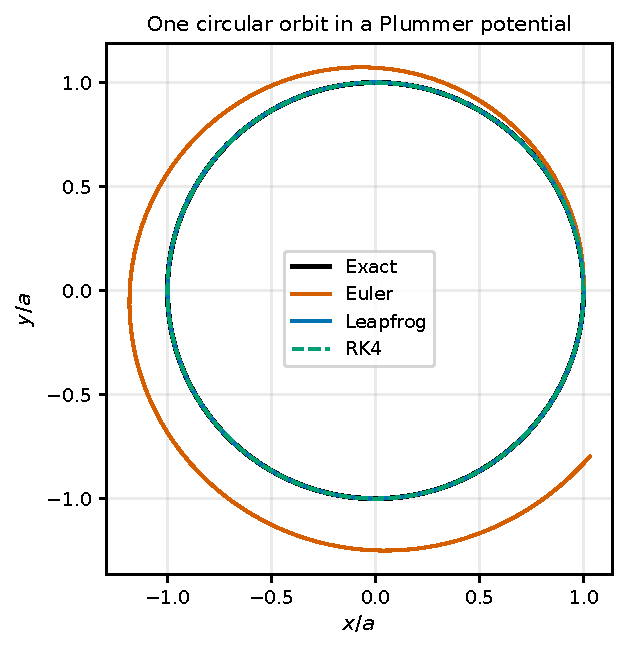
\includegraphics[width=0.62\linewidth]{ch03_circular_orbit.pdf}
\caption{1周期 $T_0$ を $N=100$ ステップで積分した円軌道。時間刻みは $\Delta t=T_0/100$ である。解析解と3つの時間積分法を比較している。}
\label{fig:ch3-circular}
\end{figure}

図\ref{fig:ch3-circular}では、Euler 法の軌道が外側へずれる一方、リープフロッグ法と RK4 は解析的な円軌道に近く見える。
ただし、一つの時間刻みで描いた軌道だけでは、誤差の大きさや収束次数を十分には判断できない。
次節では、解析解からの位置のずれを直接測り、時間刻みを変えたときの誤差の減少を調べる。
% =====================================================================
\section{時間積分法の収束次数}
\label{sec:ch3-convergence}

前節では、一つの時間刻みで1周期の軌道を描いた。
本節では終端時刻を固定し、時間刻みを変えて同じ計算を繰り返す。
第\ref{sec:ch1-convergence}節の格子収束試験で格子幅を変えたのと同じ考え方で、時間積分法の収束次数を測定する。

ここでは、円軌道を90度進んだ時刻 $T_0/4$ を終端時刻とする。この時刻の厳密な位置は
\begin{equation}
 \boldsymbol{x}_{\rm exact}(T_0/4)=(0,r_0)
\end{equation}
と分かっているので、数値的な位置とのずれ
\begin{equation}
 \epsilon_x=\left|\boldsymbol{x}_{\rm num}(T_0/4)-\boldsymbol{x}_{\rm exact}(T_0/4)\right|
\label{eq:ch3-position-error}
\end{equation}
を直接測定できる。
縦棒はベクトルの大きさを表し、$\epsilon_x$ は二つの位置の間の距離である。
コードでは \texttt{np.linalg.norm} で計算する。

Notebook 3 では、$T_0/4$ までを $N=20,40,80,160,320$ ステップで積分する。
前節の1周期の計算とは異なり、ここでの時間刻みは $\Delta t=T_0/(4N)$ である。
誤差が $\epsilon_x\simeq C(\Delta t)^p$ に従う範囲では、両対数プロットの傾きが収束次数 $p$ となる。
$C$ は、終端時刻と初期条件を固定したときに時間刻みに依存しない係数である。
\begin{notebookblock}{3｜時間積分法の収束次数}
積分関数を辞書 \texttt{methods} にまとめ、手法と時間刻みを変えて計算する。
\texttt{errors} に位置誤差を保存し、5種類の時間刻みすべてを用いて両対数上で直線近似する。

\par\smallskip\noindent\begin{minipage}{\linewidth}
{\sffamily\small\color{graytext}対応セル（誤差と収束次数の測定）}
\begin{Verbatim}[xleftmargin=2mm,fontsize=\small,frame=single,framesep=1.8mm,framerule=0.35pt,rulecolor=\color{listingframe},fillcolor=\color{listingbg}]
# 3つの積分関数を、名前と対応させて登録する
methods = {
    "Euler": integrate_euler,
    "Leapfrog": integrate_leapfrog,
    "RK4": integrate_rk4,
}

# 終端時刻を固定し、試すステップ数と解析的な位置を用意する
N_values = np.array([20, 40, 80, 160, 320])
t_end = T0 / 4.0
x_exact_end = np.array([0.0, r0])
dt_values = t_end / N_values
errors = {}

# 最終時刻の位置のずれを距離として測る
for name, method in methods.items():
    err = []
    for N_i in N_values:
        dt_i = t_end / N_i
        x_i, v_i = method(acc_plummer_model, x0, v0, dt_i, int(N_i))
        err.append(np.linalg.norm(x_i[-1] - x_exact_end))
    errors[name] = np.array(err)

# 両対数上での直線の傾きを求める
orders = {}
for name, err in errors.items():
    orders[name] = np.polyfit(np.log(dt_values), np.log(err), 1)[0]
\end{Verbatim}
\end{minipage}
\end{notebookblock}

この計算から、
\begin{equation}
 p_{\rm Euler}=\chthreeOrderEuler,\qquad
 p_{\rm leapfrog}=\chthreeOrderLeapfrog,\qquad
 p_{\rm RK4}=\chthreeOrderRKFour
\label{eq:ch3-orders}
\end{equation}
を得る。
Euler 法はほぼ1次、リープフロッグ法はほぼ2次、RK4 はほぼ4次精度で収束している。
時間刻みを半分にすると、誤差はそれぞれおよそ $1/2$、$1/4$、$1/16$ に減少する。
図\ref{fig:ch3-convergence}の点列の傾きは、この誤差の減少を表している。

\begin{figure}[!htbp]
\centering
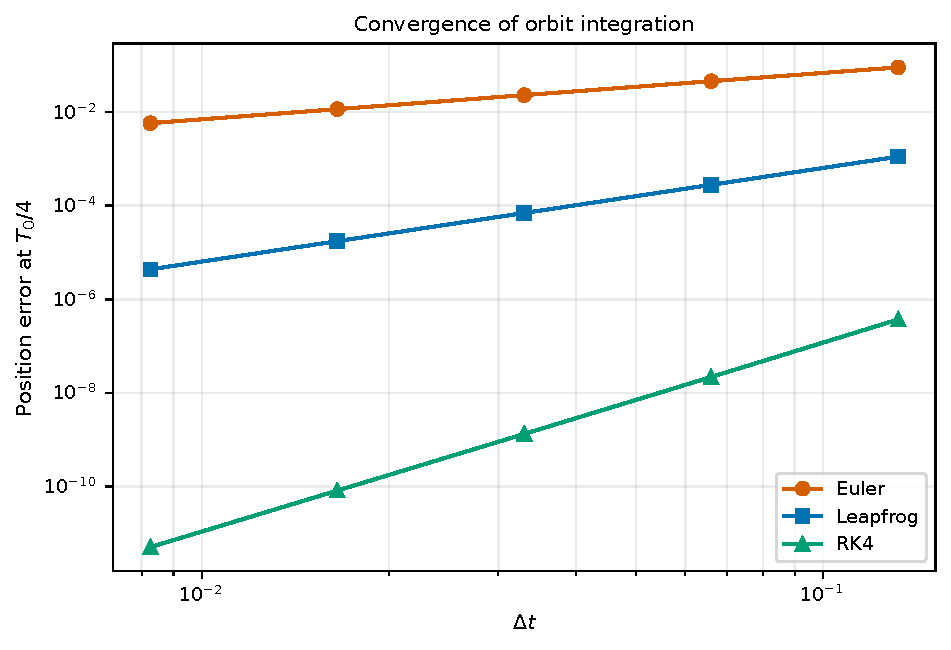
\includegraphics[width=0.66\linewidth]{ch03_convergence.pdf}
\caption{円軌道の $T_0/4$ 後の位置誤差と時間刻みの関係。両対数表示の傾きから、Euler 法・リープフロッグ法・RK4 の大域収束次数を測定する。}
\label{fig:ch3-convergence}
\end{figure}
% =====================================================================
\section{保存量による数値軌道の診断}
\label{sec:ch3-invariants}

前節では、円軌道の解析解と比較して位置の誤差を測った。
軌道計算では、このような直接比較に加えて、本来一定である保存量が数値計算でも保たれているかを調べることができる。
本節では、半径が時間とともに変化する離心軌道を用い、エネルギーと角運動量から数値軌道を診断する。

単位質量あたりのエネルギーを\textbf{比エネルギー（specific energy）}と呼び、
\begin{equation}
 E=\frac12v^2+\Phi(r)
\label{eq:ch3-energy}
\end{equation}
と定義する。ここで $v=|\boldsymbol{v}|$ である。
また、単位質量あたりの角運動量を\textbf{比角運動量（specific angular momentum）}と呼び、
\begin{equation}
 \boldsymbol{L}=\boldsymbol{x}\times\boldsymbol{v}
\label{eq:ch3-angular-momentum}
\end{equation}
と定義する。
以下では、これらを単にエネルギー、角運動量と呼ぶ。
ポテンシャルが時間に依存しないためエネルギーが保存され、球対称な重力場の力が中心方向を向くため角運動量が保存される。
したがって、厳密な運動では
\begin{equation}
 \boxed{E=\mathrm{const.},\qquad\boldsymbol{L}=\mathrm{const.}}
\label{eq:ch3-spherical-invariants}
\end{equation}
である\cite{ryden2025}。
本章の $x$--$y$ 平面内の運動では、その平面に垂直な成分 $L_z=xv_y-yv_x$ を診断に用いる。

Notebook 3 では、$G=M=a=1$ の単位で
\begin{equation}
 \boldsymbol{x}_0=(1,0),\qquad\boldsymbol{v}_0=(0,0.45)
\label{eq:ch3-eccentric-ic}
\end{equation}
とする。
初速度をこの半径の円運動速度より小さくすることで、半径が変化する軌道を作る。
$\Delta t=T_0/100$ で、基準周期の20倍の時間 $20T_0$ まで2000ステップで積分する。
$T_0$ は式\eqref{eq:ch3-plummer-period}の円軌道の基準周期であり、この離心軌道の実測周期ではない。

計算した各時刻で保存量を評価し、初期値からの相対的なずれ
\begin{equation}
 \frac{E(t)-E(0)}{|E(0)|},\qquad
 \frac{L_z(t)-L_z(0)}{|L_z(0)|}
\label{eq:ch3-relative-invariants}
\end{equation}
を求める。今回の初期条件では、どちらの分母も0ではない。
これらの量が0からどれだけずれるかを調べることで、保存量が数値計算でどの程度保たれているかを確認できる。
\begin{notebookblock}{3｜離心軌道と保存量}
前節で定義した \texttt{methods} を使い、同じ初期条件を3つの方法で積分する。
\texttt{orbits} に軌道と保存量を保存し、\texttt{relative\_errors} に式\eqref{eq:ch3-relative-invariants}の符号付きのずれを保存する。

\par\smallskip\noindent\begin{minipage}{\linewidth}
{\sffamily\small\color{graytext}対応セル（保存量を計算する関数）}
\begin{Verbatim}[xleftmargin=2mm,fontsize=\small,frame=single,framesep=1.8mm,framerule=0.35pt,rulecolor=\color{listingframe},fillcolor=\color{listingbg}]
# 全時刻の位置・速度配列から、各時刻の比エネルギーを返す
def energy_plummer(x, v, G, M, a):
    return 0.5 * np.sum(v**2, axis=1) + phi_plummer_pos(x, G, M, a)

# 平面内の運動に対する比角運動量の z 成分を返す
def angular_momentum_z(x, v):
    return x[:, 0] * v[:, 1] - x[:, 1] * v[:, 0]
\end{Verbatim}
\end{minipage}

\par\smallskip\noindent\begin{minipage}{\linewidth}
{\sffamily\small\color{graytext}対応セル（軌道と保存量の計算）}
\begin{Verbatim}[xleftmargin=2mm,fontsize=\small,frame=single,framesep=1.8mm,framerule=0.35pt,rulecolor=\color{listingframe},fillcolor=\color{listingbg}]
# 離心軌道の初期条件と計算時間を設定する
x0_e = np.array([1.0, 0.0])
v0_e = np.array([0.0, 0.45])
n_period = 20
steps_per_period = 100
dt = T0 / steps_per_period
nstep = n_period * steps_per_period
t = np.arange(nstep + 1) * dt

# 各手法の軌道と保存量の履歴を保存する
orbits = {}
for name, method in methods.items():
    x_i, v_i = method(acc_plummer_model, x0_e, v0_e, dt, nstep)
    E_i = energy_plummer(x_i, v_i, G, M, a)
    L_i = angular_momentum_z(x_i, v_i)
    orbits[name] = (x_i, v_i, E_i, L_i)
\end{Verbatim}
\end{minipage}

\par\smallskip\noindent\begin{minipage}{\linewidth}
{\sffamily\small\color{graytext}対応セル（保存量の相対変化）}
\begin{Verbatim}[xleftmargin=2mm,fontsize=\small,frame=single,framesep=1.8mm,framerule=0.35pt,rulecolor=\color{listingframe},fillcolor=\color{listingbg}]
# 符号付きの相対変化と、その絶対値の最大値を求める
relative_errors = {}
short_max_errors = {}
for name in methods:
    E_i, L_i = orbits[name][2:]
    relE = (E_i - E_i[0]) / abs(E_i[0])
    relL = (L_i - L_i[0]) / abs(L_i[0])
    relative_errors[name] = (relE, relL)
    max_E = np.max(np.abs(relE))
    max_L = np.max(np.abs(relL))
    short_max_errors[name] = {"energy": max_E, "Lz": max_L}
\end{Verbatim}
\end{minipage}
\end{notebookblock}

図\ref{fig:ch3-eccentric}に計算した軌道を示す。
Euler 法では軌道が外側へ広がる一方、リープフロッグ法と RK4 は中心付近の限られた範囲を運動する。
この違いを、保存量の変化から調べる。

\begin{figure}[!htbp]
\centering
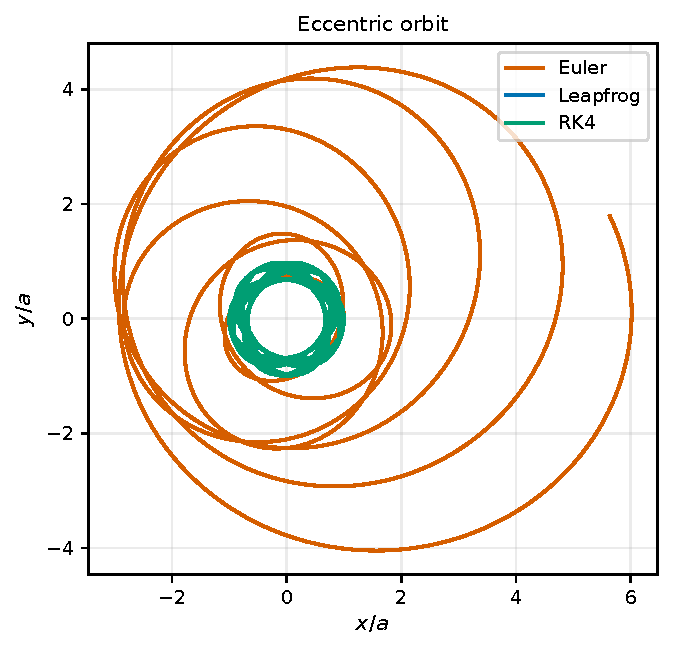
\includegraphics[width=0.52\linewidth]{ch03_eccentric_orbit.pdf}
\caption{Plummer ポテンシャル中の離心軌道。初期条件は式\eqref{eq:ch3-eccentric-ic}で、3手法を同じ $\Delta t=T_0/100$ により $20T_0$ まで積分している。}
\label{fig:ch3-eccentric}
\end{figure}

図\ref{fig:ch3-energy-error}では、式\eqref{eq:ch3-relative-invariants}のエネルギーのずれの絶対値を、対数目盛で比較している。
この時間刻みと積分時間では、最大絶対相対変化はリープフロッグ法で $\chthreeShortMaxEnergyLeapfrog$、RK4 で $\chthreeShortMaxEnergyRKFour$ となり、RK4 の方が小さい。
Euler 法の誤差はこれらより大きく、外側へ広がる軌道に対応してエネルギーも変化している。

\begin{figure}[!htbp]
\centering
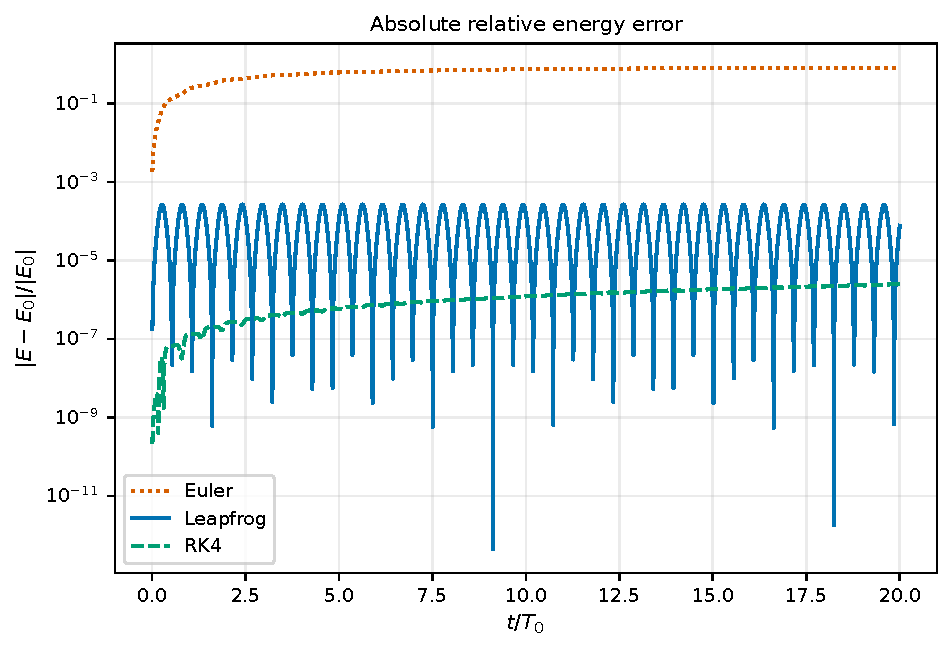
\includegraphics[width=0.65\linewidth]{ch03_energy_error.pdf}
\caption{離心軌道における $|E(t)-E(0)|/|E(0)|$。条件は $\Delta t=T_0/100$、積分時間 $20T_0$ である。縦軸は対数目盛で、誤差が0の点は表示していない。リープフロッグ法の下向きの鋭い谷は、符号付き誤差が0に近づいて絶対値が一時的に小さくなる時刻に対応し、その瞬間に軌道全体が高精度になったことを意味しない。}
\label{fig:ch3-energy-error}
\end{figure}

角運動量のずれを図\ref{fig:ch3-lz-error}に示す。
リープフロッグ法では、角運動量のずれは非常に小さい。
中心力の場合、キックで加える速度変化は位置ベクトルに平行であり、ドリフトで加える位置変化はその段階の速度に平行である。
このため、それぞれの更新で $\boldsymbol{x}\times\boldsymbol{v}$ は変わらず、角運動量は浮動小数点演算による誤差を除いて保存される。

\begin{figure}[!htbp]
\centering
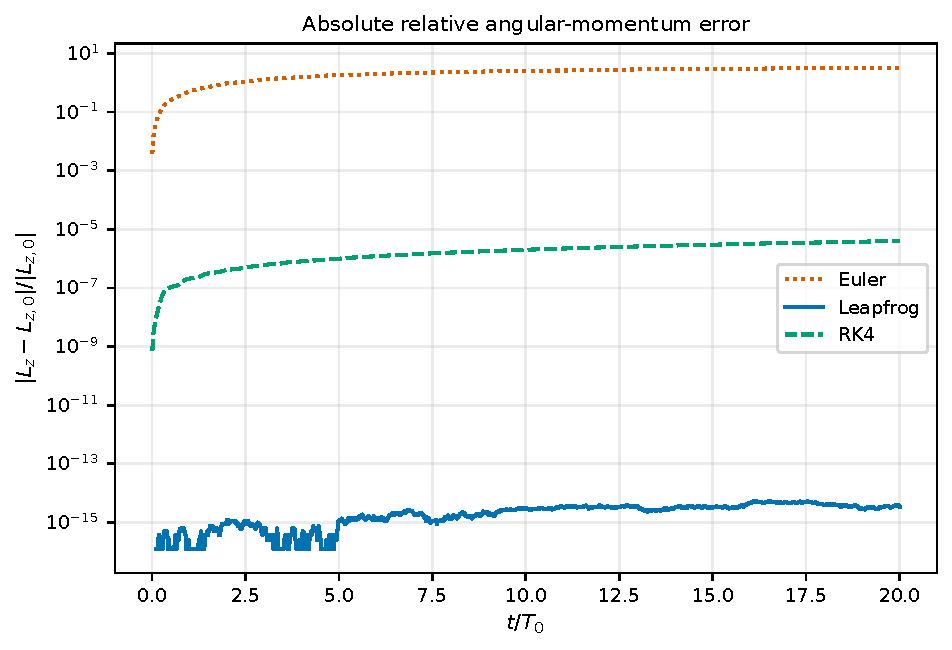
\includegraphics[width=0.65\linewidth]{ch03_angular_momentum_error.pdf}
\caption{同じ計算における $|L_z(t)-L_z(0)|/|L_z(0)|$。縦軸は対数目盛で、誤差が0の点は表示していない。
リープフロッグ法では角運動量が理論上厳密に保存されるが、実際の計算では浮動小数点演算によるわずかなずれが生じる。}
\label{fig:ch3-lz-error}
\end{figure}

ただし、角運動量が保存されていても、数値軌道が正確とは限らない。
例えば、円軌道では角運動量が一定でも、軌道位相に誤差が生じると、同じ時刻における恒星の位置は解析解からずれてしまう。
そのため、角運動量の保存だけでなく、解析解との比較や時間刻みを変えた収束試験によっても、
数値計算の精度を確かめる必要がある。

また、エネルギー誤差の大きさだけでなく、符号付きの時間変化にも違いがある。
リープフロッグ法では誤差が振動するのに対し、RK4 では一方向へのずれが見られる。
この符号付き誤差の拡大図は Notebook 3 で確認できる。
次節では、積分時間を長くして両者の違いを調べる。
% =====================================================================
保存量の選択は、解く問題によって変わる。
自己重力の $N$ 体計算では粒子間でエネルギーを交換するため、各粒子のエネルギーは一般には一定でない。
外力がなく、粒子質量が一定の孤立系では、系全体のエネルギーなどを保存量の診断に用いる\cite{tomisaka2007}。
本章で各軌道のエネルギーを調べるのは、粒子が動いても変わらない、時間に依存しない重力場を与えているためである。

\section{高次精度と長時間保存性の違い}
\label{sec:ch3-long-term}

前節の条件では、RK4 のエネルギー誤差はリープフロッグ法より小さかった。
しかし、その大小だけでは、さらに長い時間まで積分したときの誤差を判断できない。
本節では同じ離心軌道を長時間積分し、誤差が振動する場合と一方向にずれる場合の違いを比較する。

Notebook 3 では、$\Delta t=T_0/50$ で $1000T_0$ まで積分する。
$T_0$ は円軌道の基準周期である。
前節より積分時間が長いだけでなく、時間刻みも2倍なので、時間経過だけの影響を調べる際は、この長時間計算の最初の $20T_0$ と全体の $1000T_0$ を比べる。
手法間の比較は同じ時間刻みでの比較であり、同じ計算コストでの比較ではない。

符号付きのエネルギー誤差が振動する場合、最終値は計算を終えるタイミングによって変わる。
そこで、時間変化に加えて、終端時刻 $T$ までの出力時刻 $t_n$ で測った最大絶対相対変化
\begin{equation}
 \epsilon_{E,\max}(T)\equiv\max_{0\le t_n\le T}\frac{|E(t_n)-E(0)|}{|E(0)|}
\label{eq:ch3-max-energy-error}
\end{equation}
を用い、計算中に誤差がどこまで大きくなったかを比較する。
\begin{notebookblock}{3｜RK4 とリープフロッグ法の長時間挙動}
前節で定義した \texttt{x0\_e}、\texttt{v0\_e} を初期条件に用い、RK4 とリープフロッグ法で計算する。
\texttt{long\_results} には全時刻の符号付き誤差を、\texttt{long\_max\_errors} には二つの時間範囲の最大誤差を保存する。

\par\smallskip\noindent\begin{minipage}{\linewidth}
{\sffamily\small\color{graytext}対応セル（長時間積分）}
\begin{Verbatim}[xleftmargin=2mm,fontsize=\small,frame=single,framesep=1.8mm,framerule=0.35pt,rulecolor=\color{listingframe},fillcolor=\color{listingbg}]
# 基準周期あたり50ステップで、1000T0 まで積分する
n_period_long = 1000
steps_per_period_long = 50
dt_long = T0 / steps_per_period_long
nstep_long = n_period_long * steps_per_period_long
t_long = np.arange(nstep_long + 1) * dt_long

# 同じ離心軌道の符号付き相対エネルギー誤差を保存する
long_results = {}
for name in ["Leapfrog", "RK4"]:
    method = methods[name]
    x_i, v_i = method(acc_plummer_model, x0_e, v0_e, dt_long, nstep_long)
    E_i = energy_plummer(x_i, v_i, G, M, a)
    long_results[name] = (E_i - E_i[0]) / abs(E_i[0])
\end{Verbatim}
\end{minipage}

\par\smallskip\noindent\begin{minipage}{\linewidth}
{\sffamily\small\color{graytext}対応セル（最大誤差の比較）}
\begin{Verbatim}[xleftmargin=2mm,fontsize=\small,frame=single,framesep=1.8mm,framerule=0.35pt,rulecolor=\color{listingframe},fillcolor=\color{listingbg}]
# 同じ計算の最初の20T0と全体で、最大誤差を測る
n_early = 20 * steps_per_period_long
long_max_errors = {}
for name in ["Leapfrog", "RK4"]:
    err = long_results[name]
    max_early = np.max(np.abs(err[:n_early + 1]))
    max_all = np.max(np.abs(err))
    long_max_errors[name] = {"early": max_early, "all": max_all}
\end{Verbatim}
\end{minipage}

\par\smallskip\noindent\begin{minipage}{\linewidth}
{\sffamily\small\color{graytext}実行結果}
\captionsetup{hypcap=false}
\captionof{table}{同じ長時間計算から求めた $\epsilon_{E,\max}(T)$。どちらの行も $\Delta t=T_0/50$ であり、§\ref{sec:ch3-invariants}の $\Delta t=T_0/100$ とは異なる。}
\label{tab:ch3-long-energy-max}
\centering
\begin{tabular}{rcc}
\toprule
$T/T_0$ & リープフロッグ法 & RK4\\
\midrule
20 & $\chthreeLongEarlyMaxLeapfrog$ & $\chthreeLongEarlyMaxRKFour$\\
1000 & $\chthreeLongMaxLeapfrog$ & $\chthreeLongMaxRKFour$\\
\bottomrule
\end{tabular}
\end{minipage}
\end{notebookblock}

図\ref{fig:ch3-long-term}に、同じ計算の符号付き相対エネルギー誤差を示す。
リープフロッグ法では誤差がほぼ一定の範囲で振動し、RK4 ではおおむね負の方向へのずれが続く。

\begin{figure}[!htbp]
\centering
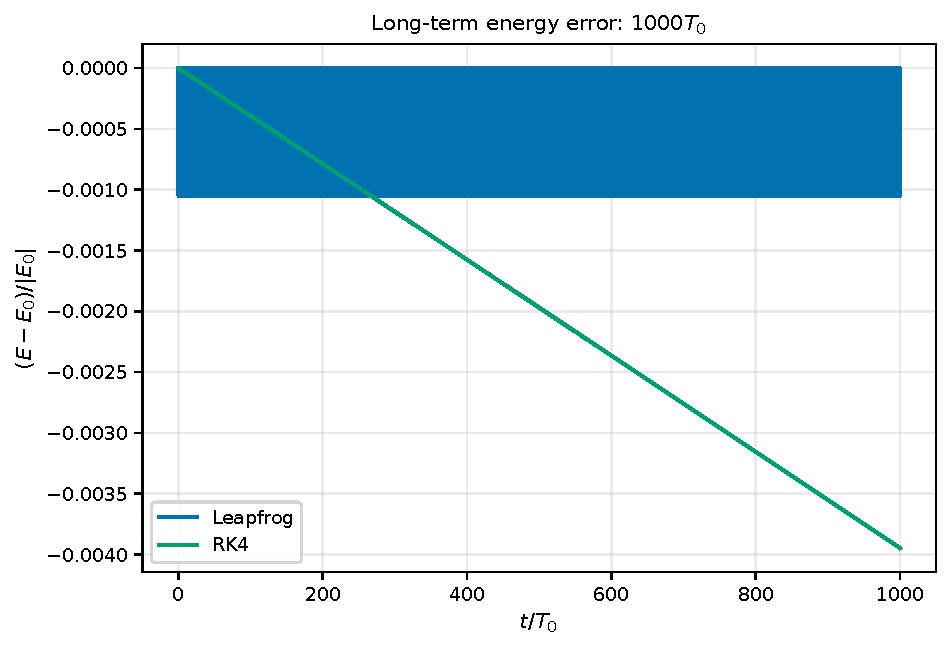
\includegraphics[width=0.68\linewidth]{ch03_long_term_energy.pdf}
\caption{$\Delta t=T_0/50$ で $1000T_0$ まで積分した符号付き相対エネルギー誤差。リープフロッグ法はほぼ一定の範囲で振動し、RK4 には負の方向への長期的なずれが見られる。多数の振動が重なるため、リープフロッグ法の曲線は帯状に見える。}
\label{fig:ch3-long-term}
\end{figure}

表\ref{tab:ch3-long-energy-max}では、リープフロッグ法の最大誤差は最初の $20T_0$ で約 $\chthreeLongEarlyMaxLeapfrog$ に達し、その後もほとんど増えない。
一方、RK4 の誤差は初めは小さいが、時間とともに増加する。
$20T_0$ までの最大誤差は RK4 の方が小さく、$1000T_0$ までではリープフロッグ法の方が小さい。
ただし、大小が入れ替わる時刻は時間刻みに強く依存する。
例えば $\Delta t=T_0/100$ では、$1000T_0$ まで積分しても RK4 の最大誤差の方が小さい。
誤差の大小を比較するときは、時間刻みと積分時間を必ず併記する必要がある。

リープフロッグ法は2次精度だが、時間に依存しない保存力による滑らかな束縛軌道を、十分小さい固定時間刻みで積分すると、エネルギー誤差が一方向に蓄積しにくい性質を持つ\cite{matsumoto}。
これは、物理的エネルギーを各ステップで厳密に保存するという意味ではない。
一方、RK4 が4次精度であることは、固定した終端時刻で時間刻みを小さくしたときの誤差の減少を表す。
収束次数と長時間の保存量の振る舞いは別の性質なので、必要な精度、積分時間、計算コストに応じて方法を選ぶことが重要である。

\begin{topicblock}{リープフロッグ法とシンプレクティック性}
リープフロッグ法の長時間挙動を理解する背景には、保存力による運動が持つ構造がある。
位置と速度を組にした状態を表す空間を\textbf{位相空間}と呼ぶ。
本章のような保存力による運動は、Hamilton 系と呼ばれる枠組みで記述できる。
この系に備わる位相空間の構造を離散的な時間更新でも保つ方法が、\textbf{シンプレクティック積分法（symplectic integrator）}であり、固定時間刻みのリープフロッグ法はその一例である。

この性質は、エネルギーを各ステップで厳密に保存することや、任意の時間刻みで安定に計算できることとは異なる。
精度の次数だけとも区別する必要がある。
実際の $N$ 体計算や SPH 計算では、粒子の状態に応じた\textbf{可変時間刻み（adaptive timestep）}や、
粒子ごとに異なる時間刻み（\textbf{独立時間刻み; individual timestep}）を用いる場合がある。
その場合、本章の共通の固定時間刻みで見た長時間の保存性はそのままでは保証されず、時間刻みの決め方と更新手順を組み合わせた検証が必要になる。

理論的背景は Notebook 3 の補足と松本ほか §9.6\cite{matsumoto}を参照する。
\end{topicblock}


\begin{topicblock}{宇宙流体計算の時間積分：RK2 と RK3}
本章で扱った時間積分は、星の軌道計算だけでなく、空間を離散化した流体の方程式にも用いられる。
例えば有限体積法では、密度・運動量密度・エネルギー密度などのセル平均値を持たせる。
全セルのこれらの量をまとめたベクトルを $\boldsymbol{U}$ とすると、空間方向を離散化した後の時間発展は
\begin{equation}
 \frac{d\boldsymbol{U}}{dt}=\boldsymbol{f}(\boldsymbol{U})
\label{eq:ch3-hydro-ode}
\end{equation}
と書ける。ここでは、右辺が時刻に明示的に依存しない場合を考える。
$\boldsymbol{f}(\boldsymbol{U})$ は、現在の状態からセル境界を通る流束や重力などの効果を評価し、各セルの時間変化率を計算する関数である。
式\eqref{eq:ch3-first-order}と同じ形なので、常微分方程式の時間積分法を適用できる。

格子法の宇宙流体計算では、2次や3次の Runge--Kutta 法も用いられる\cite{fujii2020,matsumoto}。
ここでは、その具体例として2段2次の RK2 と3段3次の RK3 を示す。
$\boldsymbol{U}^n$ は時刻 $t_n$ の数値状態を表し、上付きの $(1)$、$(2)$ は計算途中の補助状態を表す。

2次精度の Heun 法（RK2）は、
\begin{align*}
 \boldsymbol{U}^{(1)}&=\boldsymbol{U}^n+\Delta t\,\boldsymbol{f}(\boldsymbol{U}^n),\\
 \boldsymbol{U}^{n+1}&=\frac12\boldsymbol{U}^n+\frac12\left[\boldsymbol{U}^{(1)}+\Delta t\,\boldsymbol{f}(\boldsymbol{U}^{(1)})\right]
\end{align*}
と書ける。
最初に Euler 法で予測値 $\boldsymbol{U}^{(1)}$ を求め、その予測値でも時間変化率を評価する。
2行目に1行目を代入すると、始点と予測した終点での変化率を平均して更新する式になる。

代表的な3次精度の公式（RK3）では、最初の予測値 $\boldsymbol{U}^{(1)}$ は上の Heun 法と共通である。
その後、次の2段で更新する。
\begin{align*}
 \boldsymbol{U}^{(2)}&=\frac34\boldsymbol{U}^n+\frac14\left[\boldsymbol{U}^{(1)}+\Delta t\,\boldsymbol{f}(\boldsymbol{U}^{(1)})\right],\\
 \boldsymbol{U}^{n+1}&=\frac13\boldsymbol{U}^n+\frac23\left[\boldsymbol{U}^{(2)}+\Delta t\,\boldsymbol{f}(\boldsymbol{U}^{(2)})\right].
\end{align*}
ここで示した RK2 では2回、RK3 では3回、右辺の関数を評価する。
いずれも、Euler 法による予測と既知の状態との重み付き平均を組み合わせた更新として読める。

SPH 法へ拡張して速度依存の力や散逸を扱う場合には、本章の保存力に対するリープフロッグ法の保存性はそのままでは保証されない。
RK2・RK3 でも、空間離散化と組み合わせた時間刻みの制約を満たす必要がある。
詳しくは藤井・立川\cite{fujii2020}、松本ほか\cite{matsumoto}を参照すること。
\end{topicblock}

% =====================================================================

\clearpage

\appendix
\titleformat{\chapter}{\LARGE\bfseries\sffamily\color{navy}}{付録\thechapter}{0.8em}{}
\makeatletter
\renewcommand{\chaptermark}[1]{\markboth{付録\thechapter\enspace #1}{}}
\makeatother
\chapter{軸対称円盤の質量積分と回転曲線}
\label{app:disk-integrals}

第1章では、球対称な密度分布から内包質量を求め、数値積分法の精度を検証した。
本付録では、Ryden §6.5 の薄い軸対称円盤を題材として、既習の数値積分を別の問題へ適用する\cite{ryden2025}。
球殻から円環へ質量要素を変え、同じ累積台形則で指数円盤の内包質量を求める。
解析解との比較と格子収束試験によって、実装を再利用した場合も精度を確かめる。

後半では、円盤の回転曲線と球対称近似を比較する。
ここでは解析式を用い、数値積分の誤差を混ぜずに、質量分布の仮定による違いを調べる。
数値手法を再利用できることと、物理の関係式をそのまま使えることは別である。
本付録は第1章の発展内容であり、第2・3章や他の付録を先に読む必要はない。

\begin{learningbox}[本付録で学ぶこと]
\begin{itemize}
\item 軸対称円盤の質量を求める問題について、数値積分の被積分関数と積分区間を設定できる。
\item 被積分関数を入れ替え、第1章の累積台形則の実装を別の質量分布に再利用できる。
\item 解析解との比較と格子収束試験から、累積積分の誤差と収束次数を評価できる。
\item 数値積分の離散化誤差と、有限の計算領域の外にある質量を区別できる。
\item 数値計算の誤差と、物理モデルの仮定によって生じる違いを区別できる。
\end{itemize}
\end{learningbox}

数値実験は Notebook A で行う。
積分公式と累積積分の実装には、第1章で学んだものを使う\cite{kouya2021}。
本文では、被積分関数の設定、既習の実装の使い方、数値結果の検証を説明する。

\section{球対称系と軸対称円盤の質量要素}
\label{sec:appA-annulus}

球対称系では、半径 $r$、厚さ $dr$ の球殻の質量は
\begin{equation}
 dM=4\pi r^2\rho(r)\,dr
\end{equation}
であった。
一方、無限に薄い軸対称円盤では、円盤面内で中心から測った半径を $R$ とし、単位面積あたりの質量を\textbf{面密度（surface density）} $\Sigma(R)$ で表す。
半径 $R$、幅 $dR$ の薄い\textbf{円環（annulus）}の面積は、円周に幅を掛けた
\begin{equation}
 dA=2\pi R\,dR
\end{equation}
なので、その質量は
\begin{equation}
 dM=2\pi R\Sigma(R)\,dR
\label{eq:appA-annulus-mass}
\end{equation}
となる。半径 $R$ より内側の内包質量は
\begin{equation}
 \boxed{M(<R)=\int_0^R 2\pi R'\Sigma(R')\,dR'.}
\label{eq:appA-enclosed-integral}
\end{equation}
ここで $R'$ は積分変数である。
数値積分に渡す被積分関数は $\Sigma(R')$ そのものではなく、$2\pi R'\Sigma(R')$、積分区間は $[0,R]$ である。
球対称系の $4\pi r'^2\rho(r')$ をこの関数に入れ替えれば、同じ1次元の積分法を使える。

\section{指数円盤の内包質量}
\label{sec:appA-exponential}

数値積分の検証には、内包質量を解析的に求められる\textbf{指数円盤（exponential disk）}
\begin{equation}
 \Sigma(R)=\Sigma_0 e^{-R/R_d}
\label{eq:appA-surface-density}
\end{equation}
を使う。
$\Sigma_0$ は中心面密度、$R_d$ は面密度が中心値の $1/e$ になる半径である\cite{ryden2025}。

\subsection{全質量と中心面密度}

円盤の全質量を $M_d$ とすると、式\eqref{eq:appA-enclosed-integral}の上端を無限大にして
\begin{equation}
 M_d=2\pi\Sigma_0\int_0^\infty R'e^{-R'/R_d}\,dR'
\end{equation}
である。
$u=R'/R_d$ と変数変換すれば、$R'=R_du$、$dR'=R_d\,du$ なので
\begin{equation}
 M_d=2\pi\Sigma_0R_d^2\int_0^\infty ue^{-u}\,du.
\end{equation}
部分積分から
\begin{equation}
 \int ue^{-u}\,du=-ue^{-u}+\int e^{-u}\,du=-(u+1)e^{-u}+C
\label{eq:appA-antiderivative}
\end{equation}
となる。$C$ は積分定数である。
上端と下端で評価すると定積分の値は1なので、
\begin{equation}
 M_d=2\pi\Sigma_0R_d^2,\qquad \Sigma_0=\frac{M_d}{2\pi R_d^2}
\label{eq:appA-normalization}
\end{equation}
を得る。Notebook A では $M_d$ と $R_d$ を指定して $\Sigma_0$ を決める。

\subsection{有限半径までの内包質量}

同じ変数変換を有限の上端 $R$ に対して使うと、
\begin{align}
 M(<R)&=2\pi\Sigma_0R_d^2\int_0^{R/R_d}ue^{-u}\,du\notag\\
 &=M_d\left[1-e^{-R/R_d}\left(1+\frac{R}{R_d}\right)\right]
\label{eq:appA-mass-exact}
\end{align}
となる。
式\eqref{eq:appA-antiderivative}を上端と下端で評価し、式\eqref{eq:appA-normalization}を使った。
これは Ryden の式(6.161)に対応する解析解であり、$R=0$ で0、$R\to\infty$ で $M_d$ となる\cite{ryden2025}。
以下では、この式を有限半径までの数値積分を検証する基準にする。

\subsection{被積分関数と実装}

被積分関数は
\begin{equation}
 f_M(R)\equiv\frac{dM}{dR}=2\pi R\Sigma(R)=\frac{M_d}{R_d}\frac{R}{R_d}e^{-R/R_d}
\label{eq:appA-mass-integrand}
\end{equation}
である。
面密度は中心で最大だが、$f_M$ は $R=0$ で0になる。一定幅の円環の面積が中心へ向かって小さくなるためである。
図\ref{fig:appA-profiles}では、面密度と被積分関数をそれぞれの基準量で割り、半径に対する形を比較する。

\begin{figure}[!htbp]
\centering
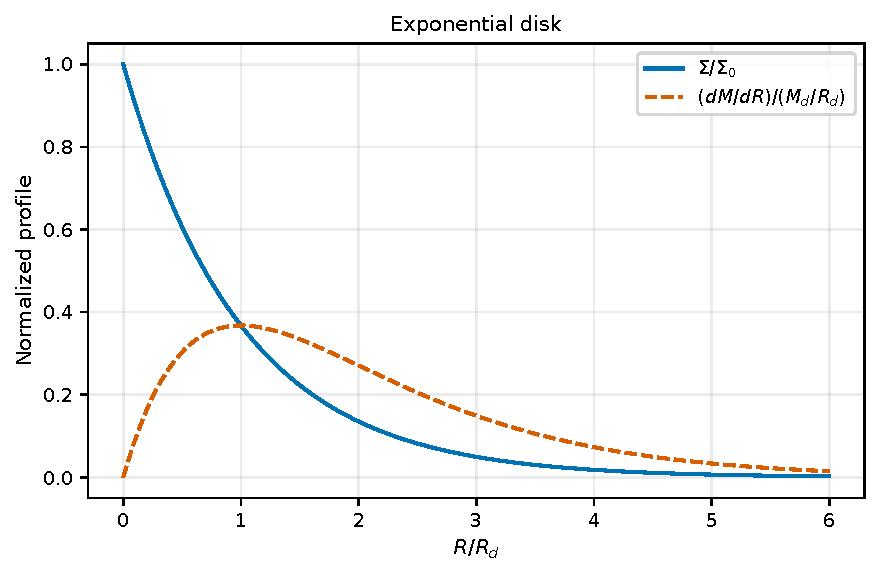
\includegraphics[width=0.64\linewidth]{appA_exponential_profiles.pdf}
\caption{指数円盤の面密度と、一定の動径幅あたりの質量。面密度は $\Sigma_0$、被積分関数 $dM/dR$ は $M_d/R_d$ で規格化した。両者は異なる物理量なので、ここでは半径に対する形の違いを比較する。}
\label{fig:appA-profiles}
\end{figure}

式\eqref{eq:appA-surface-density}と式\eqref{eq:appA-mass-integrand}を関数にすると、Listing A.1 になる。
\texttt{sigma\_exponential} が面密度、\texttt{dMdR\_exponential} が数値積分に渡す被積分関数を返す。

\begin{listingbox}{A.1　指数円盤の面密度と被積分関数}
\begin{Verbatim}[fontsize=\small]
def sigma_exponential(R, Md=1.0, Rd=1.0):
    Sigma0 = Md / (2.0 * np.pi * Rd**2)
    return Sigma0 * np.exp(-R / Rd)

def dMdR_exponential(R, Md=1.0, Rd=1.0):
    return 2.0 * np.pi * R * sigma_exponential(R, Md, Rd)
\end{Verbatim}
\end{listingbox}

\section{累積台形則による数値積分}
\label{sec:appA-cumulative}

計算領域 $0\le R\le R_{\max}$ を $N$ 個の区間に分け、
\begin{equation}
 R_i=i\Delta R,\qquad \Delta R=\frac{R_{\max}}{N},\qquad i=0,1,\ldots,N
\label{eq:appA-grid}
\end{equation}
とする。
第1章の累積台形則を $f_M$ に使えば、内包質量の数値近似 $M_i\simeq M(<R_i)$ は
\begin{equation}
 M_0=0,\qquad M_{i+1}=M_i+\frac{\Delta R}{2}\left[f_M(R_i)+f_M(R_{i+1})\right]
\label{eq:appA-cumulative-trapezoid}
\end{equation}
で求められる。$i=0,1,\ldots,N-1$ の順に更新すれば、各半径について0から積分をやり直す必要はない。

実装には第1章の Listing 1.5 の \texttt{cumulative\_trapezoid\_manual} を使う。
この関数は、引数 \texttt{x} に格子、\texttt{y} に被積分関数の値を受け取り、各区間の台形面積を \texttt{np.cumsum} で累積する。
ここでは \texttt{x} に $R_i$、\texttt{y} に $f_M(R_i)$ を渡す。
積分する関数が変わるだけで、累積加算の実装は変わらない（\S\ref{sec:ch1-cumulative}）。

\begin{notebookblock}{A｜内包質量の数値積分}
$G=M_d=R_d=1$ とし、$0\le R\le10R_d$ を400区間に分ける。
\texttt{R} は両端を含む401個の格子点である。
\texttt{mass\_exponential\_exact} は式\eqref{eq:appA-mass-exact}を返す関数で、完全な定義は Notebook A に置く。

{\sffamily\small\color{graytext}対応セル（計算部分）}
\begin{Verbatim}[xleftmargin=2mm,fontsize=\small,frame=single,framesep=1.8mm,framerule=0.35pt,rulecolor=\color{listingframe},fillcolor=\color{listingbg}]
# 0 <= R <= 10 Rd を N=400 区間に分ける
N = 400
R_max = 10.0 * Rd
R = np.linspace(0.0, R_max, N + 1)

# 被積分関数 dM/dR = 2 pi R Sigma(R) を格子点で評価する
dMdR = dMdR_exponential(R, Md, Rd)

# 累積台形則と、同じ格子点での解析解を比較する
M_num = cumulative_trapezoid_manual(R, dMdR)
M_exact = mass_exponential_exact(R, Md, Rd)

# 積分誤差と、計算領域の外にある質量を別々に測る
mass_error_outer = (M_num[-1] - M_exact[-1]) / Md
mass_outside = (Md - M_exact[-1]) / Md
\end{Verbatim}
\end{notebookblock}

同じ格子点で得た数値解と解析解を図\ref{fig:appA-mass-profile}に示す。
二つの曲線はほぼ重なり、外側の格子点では
\begin{equation}
 \frac{M_{\rm num}(<R_{\max})}{M_d}=\appAMassRmaxNum,\qquad
 \frac{M_{\rm exact}(<R_{\max})}{M_d}=\appAMassRmaxExact
\label{eq:appA-mass-at-rmax}
\end{equation}
となる。
両者の差が、同じ上端まで積分したときの数値積分の誤差である。

\begin{figure}[!htbp]
\centering
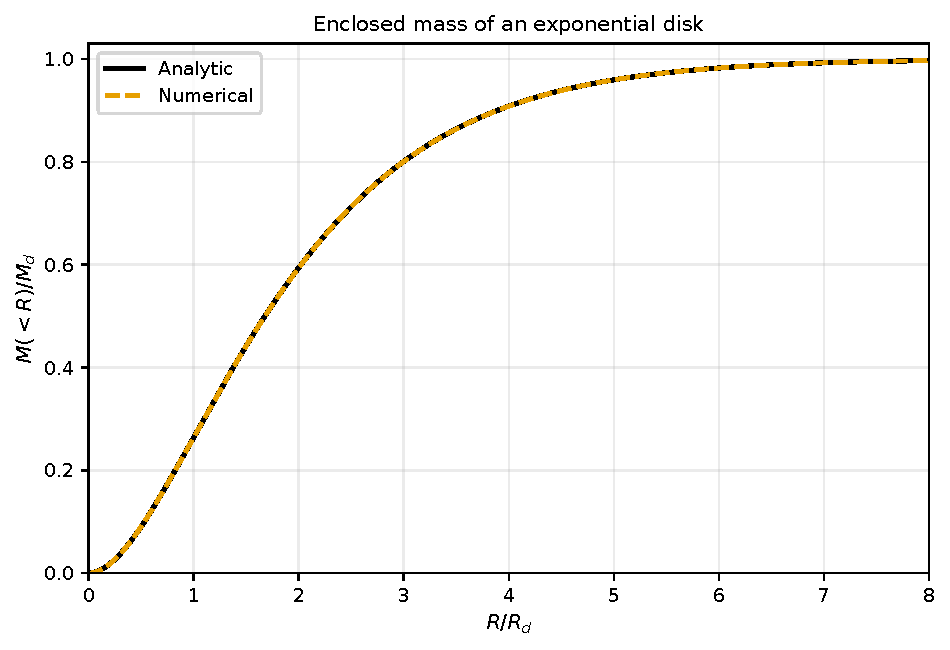
\includegraphics[width=0.64\linewidth]{appA_mass_profile.pdf}
\caption{指数円盤の内包質量の解析解と累積台形積分。計算は $0\le R\le10R_d$ を400区間に分けて行い、図には $R\le8R_d$ の範囲を示す。質量は円盤の全質量 $M_d$ で規格化している。}
\label{fig:appA-mass-profile}
\end{figure}

\subsection{積分誤差と計算領域の外にある質量}

一方、解析解でも $M_{\rm exact}(<R_{\max})<M_d$ である。
その差は数値積分の誤差ではなく、計算領域の外にある質量であり、式\eqref{eq:appA-mass-exact}から
\begin{equation}
 \frac{M_d-M_{\rm exact}(<R_{\max})}{M_d}
 =e^{-R_{\max}/R_d}\left(1+\frac{R_{\max}}{R_d}\right)
\label{eq:appA-mass-outside}
\end{equation}
と求められる。
$R_{\max}$ を固定したまま格子を細かくすると、数値解はその上端までの解析解へ近づくが、領域外の質量は変わらない。
全質量 $M_d$ を有限半径までの積分で近似する場合には、積分の離散化誤差とは別に、この寄与も考える必要がある。

\section{累積台形則の格子収束}
\label{sec:appA-convergence}

一つの格子で解析解と重なるだけでは、誤差が期待した次数で減るかは分からない。
計算領域を $R_{\max}=10R_d$ に固定し、全格子点での誤差を
\begin{equation}
 \epsilon_M\equiv\max_{0\le i\le N}\frac{|M_{\rm num}(<R_i)-M_{\rm exact}(<R_i)|}{M_d}
\label{eq:appA-mass-error}
\end{equation}
で測る。
これは全質量 $M_d$ で規格化した最大絶対誤差であり、各点の内包質量に対する相対誤差ではない。
一定の $M_d$ を分母に使うことで、内包質量が0の中心も評価に含められる。

第1章で学んだ台形則の誤差評価から、滑らかな被積分関数を固定区間で積分すると、離散化誤差が支配する範囲では
\begin{equation}
 \epsilon_M\simeq C\left(\frac{\Delta R}{R_d}\right)^p,\qquad p=2
\label{eq:appA-convergence-law}
\end{equation}
が期待される。ここで $C$ は格子幅によらない係数である。
累積積分でも、各上端まで同じ台形則で積分するため、この誤差評価を使える。
$R_d$ を固定しているので、$\log\Delta R$ に対する $\log\epsilon_M$ の傾きも $p$ となる。

\noindent\textbf{検証手順｜累積台形則の格子収束}
\begin{enumerate}
\item 計算領域と $M_d,R_d$ を固定し、区間数を $N=25,50,100,200,400,800$ と変える。
\item 各格子で累積積分と解析解を比較し、式\eqref{eq:appA-mass-error}の最大誤差を測る。
\item 両対数で誤差が規則的に減少する範囲を確かめ、その傾きを2と比較する。
\end{enumerate}

\begin{notebookblock}{A｜累積台形則の格子収束}
\texttt{exponential\_mass\_error} は1つの格子の幅と最大誤差を返す。
区間数を2倍ずつ増やし、格子幅を半分にして計算を繰り返す。

{\sffamily\small\color{graytext}対応セル（計算部分）}
\begin{Verbatim}[xleftmargin=2mm,fontsize=\footnotesize,frame=single,framesep=1.8mm,framerule=0.35pt,rulecolor=\color{listingframe},fillcolor=\color{listingbg}]
# 1つの格子で内包質量の最大誤差を測る
def exponential_mass_error(N, R_max=10.0, Md=1.0, Rd=1.0):
    R = np.linspace(0.0, R_max, N + 1)
    dMdR = dMdR_exponential(R, Md, Rd)
    M_num = cumulative_trapezoid_manual(R, dMdR)
    M_exact = mass_exponential_exact(R, Md, Rd)
    dR = R[1] - R[0]
    err = np.max(np.abs(M_num - M_exact)) / Md
    return dR, err

# 領域とモデルを固定し、区間数を2倍ずつ増やす
N_values = np.array([25, 50, 100, 200, 400, 800])
dR_values = []
mass_errors = []
for N_i in N_values:
    dR_i, err_i = exponential_mass_error(int(N_i), 10.0 * Rd, Md, Rd)
    dR_values.append(dR_i)
    mass_errors.append(err_i)

dR_values = np.array(dR_values)
mass_errors = np.array(mass_errors)

# log(error)-log(dR) の直線の傾きが収束次数 p
order_mass = np.polyfit(np.log(dR_values), np.log(mass_errors), 1)[0]
\end{Verbatim}
\end{notebookblock}

図\ref{fig:appA-mass-convergence}では、6格子の誤差がほぼ2次の傾きで減少している。
これらすべての点を両対数で直線近似すると、
\begin{equation}
 p=\appAMassOrder
\label{eq:appA-mass-order}
\end{equation}
を得る。
球対称系から円盤へ題材を変えても、累積台形則の約2次の収束を確認できる。
格子をさらに細かくする場合も、当てはめには離散化誤差が規則的に減少する範囲を使い、丸め誤差で停滞した点や誤差が0の点は含めない。

\begin{figure}[!htbp]
\centering
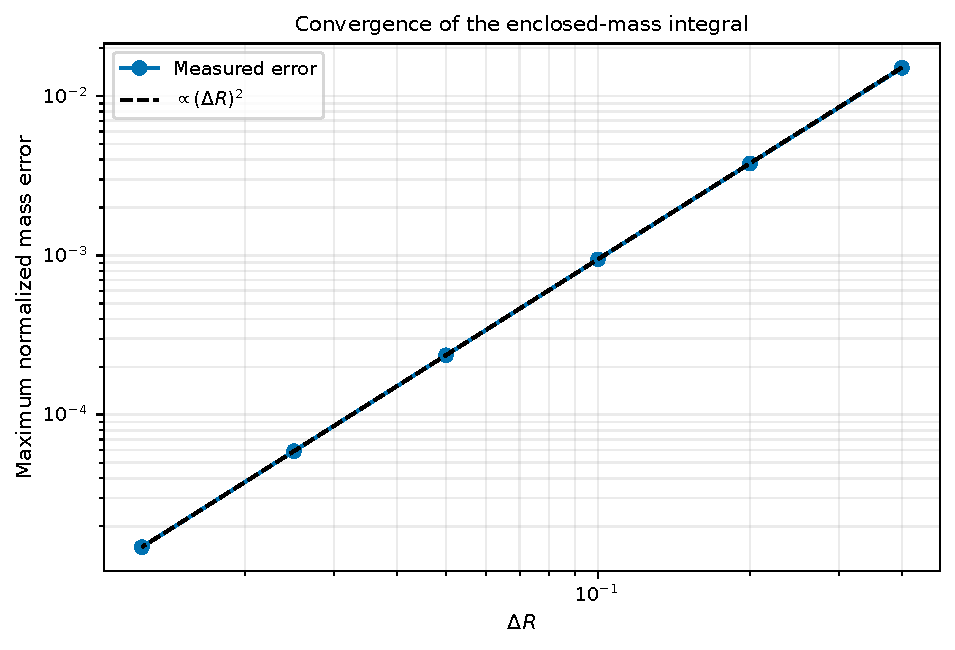
\includegraphics[width=0.64\linewidth]{appA_mass_convergence.pdf}
\caption{指数円盤の累積台形積分の格子収束。縦軸は式\eqref{eq:appA-mass-error}の誤差、横軸は $R_d=1$ の単位での格子幅である。破線は最も細かい格子での誤差を基準にした $(\Delta R)^2$ の線である。}
\label{fig:appA-mass-convergence}
\end{figure}

\section{指数円盤の回転曲線と球対称近似}
\label{sec:appA-rotation}

ここまでは、同じ積分問題に対する数値解と解析解の差を調べた。
次に、物理モデルの仮定によって結果がどう変わるかを見る。
第1章の球対称系では、Newton の球殻定理から
\begin{equation}
 v_{\rm circ}^2(r)=\frac{GM(<r)}{r}
\end{equation}
と書けた。
しかし円盤面内では、半径 $R$ より外側の質量も重力に寄与する。
球殻のように外側の質量の寄与が打ち消し合うわけではないため、その半径より内側の総質量だけでは円運動速度を決められない。

薄い指数円盤の回転曲線は、\textbf{修正 Bessel 関数（modified Bessel functions）}を用いて
\begin{equation}
 v_{\rm disk}^2(R)=4\pi G\Sigma_0R_d\,y^2\left[I_0(y)K_0(y)-I_1(y)K_1(y)\right],
 \qquad y=\frac{R}{2R_d}
\label{eq:appA-disk-rotation}
\end{equation}
と表せる。
$I_n$ と $K_n$ は、それぞれ第1種・第2種の $n$ 次修正 Bessel 関数であり、ここでは $n=0,1$ を使う。
この式は、Ryden の式(6.149)にある薄い円盤の Hankel 積分を指数円盤について評価した形に対応する。Ryden の図6.6には、その回転曲線が示されている\cite{ryden2025}。
本付録では式\eqref{eq:appA-disk-rotation}の導出には立ち入らず、比較に使う解析式として扱う。
Notebook A では \texttt{scipy.special.iv} と \texttt{kv} で関数値を求める。Hankel 積分を直接数値積分する方法は本書では扱わない。

比較曲線は、同じ内包質量を球対称分布のものとみなして
\begin{equation}
 v_{\rm sph}^2(R)\equiv\frac{GM_{\rm exact}(<R)}{R}
\label{eq:appA-spherical-comparison}
\end{equation}
と定義する。
内包質量には数値積分値ではなく解析解を使い、累積台形則の誤差を比較に混ぜない。
二つの曲線の違いは、数値積分法ではなく、質量分布を球対称とみなすことによって生じる。

\begin{notebookblock}{A｜指数円盤と球対称近似の比較}
$10^{-4}R_d\le R\le6R_d$ に等間隔の4000点を置き、二つの解析式を同じ半径で評価する。
\texttt{np.argmax} で、それぞれの最大値をとる格子点を選ぶ。作図と出力の整形は Notebook A に置く。

{\sffamily\small\color{graytext}対応セル（計算部分）}
\begin{Verbatim}[xleftmargin=2mm,fontsize=\footnotesize,frame=single,framesep=1.8mm,framerule=0.35pt,rulecolor=\color{listingframe},fillcolor=\color{listingbg}]
from scipy.special import iv, kv

# 回転曲線を評価する半径と y = R/(2 Rd)
R_rot = np.linspace(1.0e-4 * Rd, 6.0 * Rd, 4000)
y = R_rot / (2.0 * Rd)

# 修正 Bessel 関数による解析式を評価する
Bessel_term = iv(0, y) * kv(0, y) - iv(1, y) * kv(1, y)
vc2_disk = 4.0 * np.pi * G * Sigma0 * Rd * y**2 * Bessel_term

# 解析的な内包質量から球対称の比較曲線を作る
M_rot = mass_exponential_exact(R_rot, Md, Rd)
vc2_sph = G * M_rot / R_rot

# それぞれの最大値をとる格子点を求める
i_disk = np.argmax(vc2_disk)
i_sph = np.argmax(vc2_sph)
Rpeak_disk = R_rot[i_disk]
Rpeak_sph = R_rot[i_sph]
vc2peak_disk = vc2_disk[i_disk]
vc2peak_sph = vc2_sph[i_sph]
\end{Verbatim}
\end{notebookblock}

表\ref{tab:appA-rotation-peaks}に結果を示す。
$R_{\rm peak}$ は最大値をとる格子点の半径、$v_{\rm peak}$ はそこでの円運動速度である。
補間や最適化によって連続的な最大位置を求めた値ではない。
球対称近似では、最大位置が内側へずれ、最大速度も小さくなる。

\begin{table}[!htbp]
\centering
\caption{指数円盤の回転曲線と、同じ内包質量を用いた球対称近似の比較。速度の二乗は $GM_d/R_d$ で規格化している。}
\label{tab:appA-rotation-peaks}
\begin{tabular}{lcc}
\toprule
重力場のモデル & $R_{\rm peak}/R_d$ & $v_{\rm peak}^2/(GM_d/R_d)$\\
\midrule
指数円盤 & $\appADiskPeakR$ & $\appADiskPeakVTwo$\\
球対称近似 & $\appASphPeakR$ & $\appASphPeakVTwo$\\
\bottomrule
\end{tabular}
\end{table}

この違いは、回転曲線を評価する点を増やしてもなくならない。
数値積分が高い精度でできることと、物理の関係式が対象に適用できることは、分けて判断する必要がある。
図\ref{fig:appA-rotation}の実線と破線は、両曲線を共通の値 $v_{\rm max,disk}^2$ で割って示す。各曲線をそれぞれの最大値で割ったものではないので、振幅の違いも比較できる。

\section{Mestel 円盤と平坦な回転曲線}
\label{sec:appA-mestel}

一つのモデルで関係式が成り立っても、他のモデルで使えるとは限らない。
面密度が $\Sigma(R)\propto1/R$ の Mestel 円盤では、$2\pi R\Sigma(R)$ が一定なので、
\begin{equation}
 M(<R)\propto R,\qquad \frac{GM(<R)}{R}=\mathrm{const.}
\end{equation}
となる。
無限に広がる Mestel 円盤では、円盤の重力場から求めた円運動速度も一定であり、$v_{\rm circ}^2=GM(<R)/R$ が成立する。
ただし、これはこの分布に特有の結果であり、一般の円盤に使える関係ではない。

Ryden の式(6.150)では有限半径で打ち切ったモデルを導入し、式(6.158)--(6.159)で無限円盤との違いを説明している\cite{ryden2025}。
有限半径で打ち切ると、外側の質量の寄与が変わり、端の影響によって同じ等式は厳密には成り立たない。
本付録と Notebook A では有限 Mestel 円盤の重力場は計算せず、無限円盤の平坦な回転曲線を形の比較にだけ使う。

\begin{figure}[!htbp]
\centering
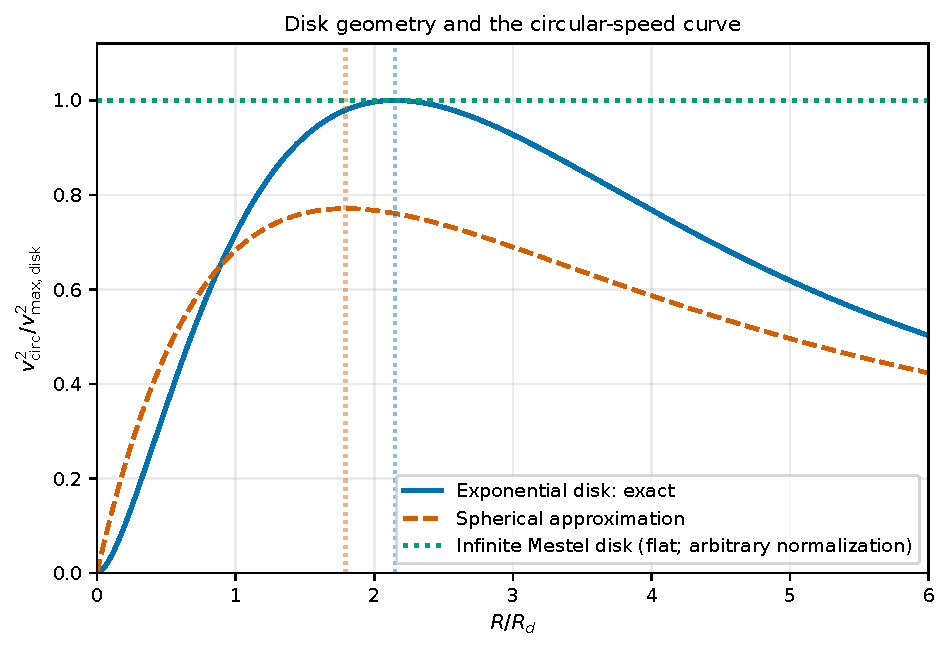
\includegraphics[width=0.69\linewidth]{appA_rotation_curve.pdf}
\caption{指数円盤の回転曲線と球対称近似。縦軸は速度の二乗を指数円盤の最大値 $v_{\rm max,disk}^2$ で割ったもので、表\ref{tab:appA-rotation-peaks}の規格化とは異なる。Mestel 円盤の点線は、無限円盤の平坦な形を示す任意規格化の線である。}
\label{fig:appA-rotation}
\end{figure}

\begin{cautionblock}{Mestel 円盤の比較線は任意規格化である}
図\ref{fig:appA-rotation}の点線は、指数円盤と同じ全質量や長さスケールから計算したものではない。
平坦な回転曲線の形を示すため、指数円盤の最大値に合わせている。
有限 Mestel 円盤の計算結果や、指数円盤と振幅まで物理的に対応する曲線として解釈してはいけない。
\end{cautionblock}


\chapter{軸対称 Poisson 方程式の数値解法}
\label{app:axisym-poisson}

第2章では、球対称 Poisson 方程式を1次元の境界値問題として解き、有限差分法の精度を検証した。
本付録では、Ryden §6.5 の軸対称系を題材として、同じ中心差分の考え方を $(R,z)$ の2次元格子へ広げる\cite{ryden2025}。
2次元 Poisson 方程式の数値解法は、本書で加えた数値計算上の発展である。
近傍点を結ぶ差分式から疎行列を構成し、境界条件を組み込んで解く手順を学ぶ。

検証には、密度とポテンシャルの解析式が分かる Miyamoto--Nagai モデルを使う。
対称軸の処理と格子点の番号付けを確認したうえで、解析解との比較、残差、格子収束試験によって結果を判断する。
本付録は第2章の発展内容であり、第3章や付録\ref{app:orbit-applications}の軌道計算の前提ではない。

\begin{learningbox}[本付録で学ぶこと]
\begin{itemize}
\item 軸対称 Poisson 方程式を、計算領域と境界条件を定めた2次元の境界値問題として設定できる。
\item 中心差分を2次元へ拡張し、対称軸での滑らかさを使って軸上の差分式を導ける。
\item 格子点と未知数番号を対応させ、既知の境界値を右辺に組み込んだ疎行列の連立一次方程式を構成できる。
\item 解析解との比較と格子収束試験から、2次元有限差分解の誤差と収束次数を評価できる。
\item 残差とポテンシャルの誤差を区別し、境界条件の近似誤差を除いて離散化誤差を検証する理由を説明できる。
\end{itemize}
\end{learningbox}

数値実験は、単独で実行できる Notebook B で行う。
本文では差分式と短い実装の対応を示し、完全なソルバーと作図は Notebook に置く。
数値計算法は幸谷第8章と§14.2.3の疎行列・2次元 Poisson 方程式の説明を参考にする\cite{kouya2021}。

\section{軸対称 Poisson 方程式と検証用モデル}
\label{sec:appB-2d-poisson-intro}

円筒座標 $(R,\phi,z)$ で軸対称性 $\partial/\partial\phi=0$ を仮定すると、Poisson 方程式は
\begin{equation}
 \boxed{\frac{\partial^2\Phi}{\partial R^2}+\frac{1}{R}\frac{\partial\Phi}{\partial R}+\frac{\partial^2\Phi}{\partial z^2}=4\pi G\rho(R,z)}
\label{eq:appB-axisym-poisson}
\end{equation}
となる。
球対称の場合と異なり、$R$ だけでなく $z$ による変化も求める必要がある。
既知の密度 $\rho(R,z)$ を右辺に与え、境界条件と合わせて未知の $\Phi(R,z)$ を決める。

\subsection{検証用の Miyamoto--Nagai モデル}

密度とポテンシャルの両方が解析的に分かれば、密度を入力として得た数値解を、ポテンシャルの解析式と比較できる。
ここでは、全質量を $M$、長さのパラメータを $a>0$、$b>0$ とする Miyamoto--Nagai モデルを使う。
\begin{equation}
 B\equiv\sqrt{z^2+b^2}
\end{equation}
とおくと、ポテンシャルは
\begin{equation}
 \Phi(R,z)=-\frac{GM}{\sqrt{R^2+(a+B)^2}}
\label{eq:appB-mn-potential}
\end{equation}
であり、対応する密度は
\begin{equation}
 \rho(R,z)=\frac{b^2M}{4\pi}\frac{aR^2+(a+3B)(a+B)^2}{B^3\left[R^2+(a+B)^2\right]^{5/2}}
\label{eq:appB-mn-density}
\end{equation}
である。
$b>0$ とすることで、対称軸と円盤面を含めて滑らかなモデルを扱う。

Notebook B の既定値は
\begin{equation}
 G=M=a=1,\qquad b=0.25
\label{eq:appB-mn-units}
\end{equation}
である。
以下では、長さの基準を $a$、ポテンシャルの基準を $GM/a$ として結果を示す。
図\ref{fig:appB-mn-density}に、この設定での密度分布を示す。

\begin{figure}[!htbp]
\centering
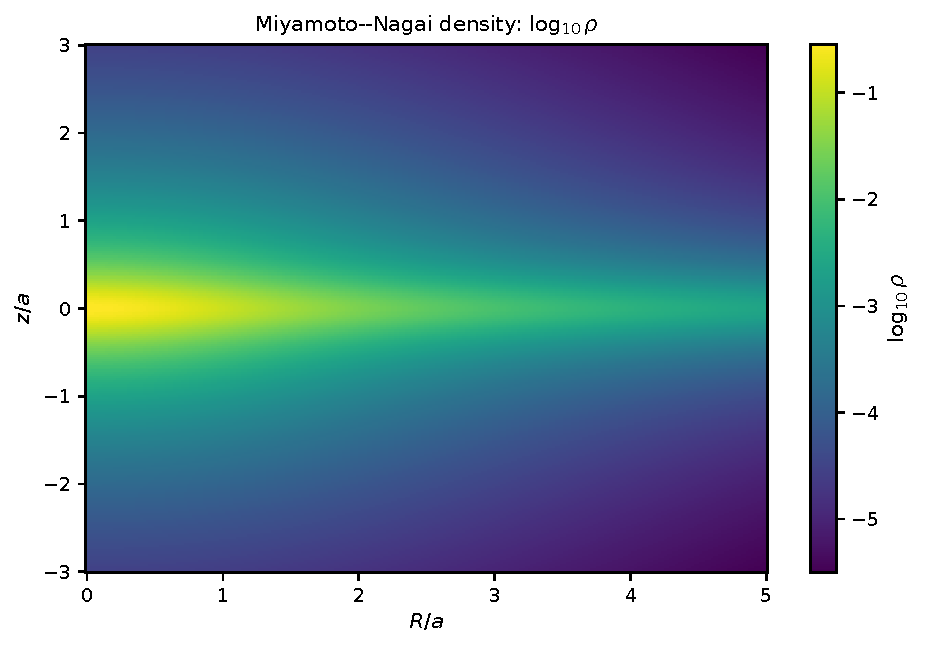
\includegraphics[width=0.64\linewidth]{appB_mn_density.pdf}
\caption{検証用の Miyamoto--Nagai モデルの密度分布。式\eqref{eq:appB-mn-units}の設定で $\log_{10}\rho$ を表示した。密度は $R$ と $z$ の両方に依存する。この図の描画用格子と、Poisson 方程式を解く格子は別に用意する。}
\label{fig:appB-mn-density}
\end{figure}

\section{2次元有限差分}
\label{sec:appB-fdm}

計算領域を $0\le R\le R_{\max}$、$-Z_{\max}\le z\le Z_{\max}$ とする。
$R$ 方向を $N_R$ 区間、$z$ 方向を $N_Z$ 区間に分け、
\begin{equation}
 \Delta R=\frac{R_{\max}}{N_R},\qquad \Delta z=\frac{2Z_{\max}}{N_Z}
\label{eq:appB-grid-spacing}
\end{equation}
とおく。両端を含む格子点は
\begin{equation}
 R_i=i\Delta R\quad(i=0,\ldots,N_R),\qquad z_j=-Z_{\max}+j\Delta z\quad(j=0,\ldots,N_Z)
\label{eq:appB-grid}
\end{equation}
である。
$N_R,N_Z$ は格子点数ではなく区間数であり、全格子点数は $(N_R+1)(N_Z+1)$ となる。
格子点上の関数値を $\Phi_{i,j}=\Phi(R_i,z_j)$ と書く。

第2章の3点ステンシル（定義2.2）を各方向へ適用する。
$R_i>0$ の内部点では、中心点と上下左右の4点を使う5点ステンシルになる（図\ref{fig:appB-stencil}）。

\subsection{$R_i>0$ の内部点}

第2章で導いた中心差分を $R$ 方向と $z$ 方向に用いると、
\begin{align}
 \left.\frac{\partial^2\Phi}{\partial R^2}\right|_{i,j}&=\frac{\Phi_{i+1,j}-2\Phi_{i,j}+\Phi_{i-1,j}}{(\Delta R)^2}+O((\Delta R)^2),\label{eq:appB-drr}\\
 \left.\frac{\partial\Phi}{\partial R}\right|_{i,j}&=\frac{\Phi_{i+1,j}-\Phi_{i-1,j}}{2\Delta R}+O((\Delta R)^2),\label{eq:appB-dr}\\
 \left.\frac{\partial^2\Phi}{\partial z^2}\right|_{i,j}&=\frac{\Phi_{i,j+1}-2\Phi_{i,j}+\Phi_{i,j-1}}{(\Delta z)^2}+O((\Delta z)^2)\label{eq:appB-dzz}
\end{align}
である。
式\eqref{eq:appB-axisym-poisson}へ代入し、打ち切り誤差を除くと、解くべき差分方程式は
\begin{equation}
 c_-\Phi_{i-1,j}+c_0\Phi_{i,j}+c_+\Phi_{i+1,j}+c_z\Phi_{i,j-1}+c_z\Phi_{i,j+1}=4\pi G\rho_{i,j}
\label{eq:appB-five-point-row}
\end{equation}
となる。以下の差分方程式で求める $\Phi_{i,j}$ は、連続なポテンシャルの数値近似である。
各点に掛かる係数をまとめると、
\begin{align}
 c_-&=\frac{1}{(\Delta R)^2}-\frac{1}{2R_i\Delta R},\label{eq:appB-cm}\\
 c_+&=\frac{1}{(\Delta R)^2}+\frac{1}{2R_i\Delta R},\label{eq:appB-cp}\\
 c_z&=\frac{1}{(\Delta z)^2},\label{eq:appB-cz}\\
 c_0&=-\frac{2}{(\Delta R)^2}-\frac{2}{(\Delta z)^2}\label{eq:appB-c0}
\end{align}
である。
動径方向では $(1/R)\partial\Phi/\partial R$ の項があるため、内側と外側の係数 $c_-,c_+$ は異なる。

\begin{figure}[!htbp]
\centering
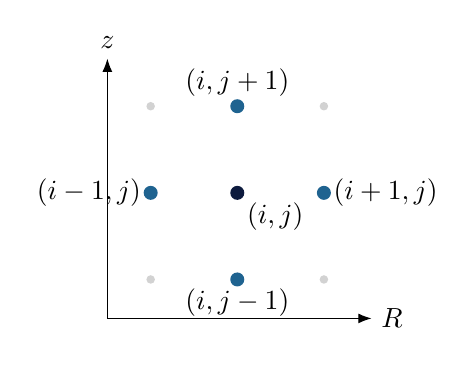
\begin{tikzpicture}[scale=1.1]
  \foreach \x in {-1,0,1}{
    \foreach \y in {-1,0,1}{
      \fill[gray!35] (\x,\y) circle (1.4pt);
    }
  }
  \fill[navy] (0,0) circle (2.3pt);
  \fill[cyan] (1,0) circle (2.3pt);
  \fill[cyan] (-1,0) circle (2.3pt);
  \fill[cyan] (0,1) circle (2.3pt);
  \fill[cyan] (0,-1) circle (2.3pt);
  \draw[->,>=Latex] (-1.5,-1.45)--(1.55,-1.45) node[right] {$R$};
  \draw[->,>=Latex] (-1.5,-1.45)--(-1.5,1.55) node[above] {$z$};
  \node[below right] at (0,0) {$(i,j)$};
  \node[right] at (1,0) {$(i+1,j)$};
  \node[left] at (-1,0) {$(i-1,j)$};
  \node[above] at (0,1) {$(i,j+1)$};
  \node[below] at (0,-1) {$(i,j-1)$};
\end{tikzpicture}
\caption{内部格子点の5点ステンシル。差分方程式は中心点と上下左右の近傍点だけを結合する。}
\label{fig:appB-stencil}
\end{figure}

Listing B.1 では、まず $z$ 方向の中心係数を設定し、$R$ 方向の寄与を加える。
\texttt{cm}, \texttt{cp}, \texttt{cz}, \texttt{center} が、それぞれ $c_-,c_+,c_z,c_0$ に対応する。

\begin{listingbox}{B.1　内部点の差分係数}
\begin{Verbatim}[fontsize=\small]
cz = 1.0 / dz**2
center = -2.0 / dz**2
cp = 1.0 / dR**2 + 1.0 / (2.0 * Ri * dR)
cm = 1.0 / dR**2 - 1.0 / (2.0 * Ri * dR)
center += -2.0 / dR**2
\end{Verbatim}
\end{listingbox}

\subsection{対称軸 $R=0$ の処理}

式\eqref{eq:appB-axisym-poisson}の $(1/R)\partial\Phi/\partial R$ を、そのまま $R=0$ で計算することはできない。
軸上でも滑らかな軸対称ポテンシャルでは
\begin{equation}
 \left.\frac{\partial\Phi}{\partial R}\right|_{R=0}=0
\label{eq:appB-axis-symmetry}
\end{equation}
なので、この項は $0/0$ の形になる。軸へ近づく極限を先に求め、有限な式に置き換える。

$z$ を固定し、対称軸を横切る直線上に符号付き座標 $\ell$ を取ると、$R=|\ell|$ である。
軸対称性によって $\ell$ と $-\ell$ の値は等しい。
第2章§\ref{sec:ch2-boundaries}と同じく、滑らかな関数の Taylor 展開には偶数次の項だけが残るため、
\begin{equation}
 \Phi(R,z)=\Phi(0,z)+\frac{1}{2}\Phi_{RR}(0,z)R^2+O(R^4)
\label{eq:appB-axis-expansion}
\end{equation}
と書ける。ここで $\Phi_{RR}$ は $R$ による二階微分である。
$R$ で微分して $R$ で割ると、
\begin{equation}
 \frac{1}{R}\frac{\partial\Phi}{\partial R}=\Phi_{RR}(0,z)+O(R^2)
\end{equation}
なので、動径方向の二つの項を合わせた極限は
\begin{equation}
 \left[\frac{\partial^2\Phi}{\partial R^2}+\frac{1}{R}\frac{\partial\Phi}{\partial R}\right]_{R=0}=2\Phi_{RR}(0,z)
\label{eq:appB-axis-limit}
\end{equation}
となる。

さらに、対称性を用いて仮想点を $\Phi_{-1,j}=\Phi_{1,j}$ とすれば、
\begin{equation}
 \Phi_{RR}(0,z_j)=\frac{\Phi_{1,j}-2\Phi_{0,j}+\Phi_{-1,j}}{(\Delta R)^2}+O((\Delta R)^2)=\frac{2(\Phi_{1,j}-\Phi_{0,j})}{(\Delta R)^2}+O((\Delta R)^2)
\end{equation}
である。したがって、軸上で動径方向の演算子全体を近似する式は
\begin{equation}
 \boxed{2\Phi_{RR}(0,z_j)\simeq\frac{4(\Phi_{1,j}-\Phi_{0,j})}{(\Delta R)^2}}
\label{eq:appB-axis-fd}
\end{equation}
となる。この差分も、軸上での滑らかさのもとで2次精度である。
$z$ 方向の中心差分を加えた軸上の差分方程式は
\begin{align}
 \left[-\frac{4}{(\Delta R)^2}-\frac{2}{(\Delta z)^2}\right]\Phi_{0,j}+\frac{4}{(\Delta R)^2}\Phi_{1,j}\notag\\
 {}+c_z\Phi_{0,j-1}+c_z\Phi_{0,j+1}=4\pi G\rho_{0,j}
\label{eq:appB-axis-row}
\end{align}
である。

Listing B.2 は、Listing B.1 の動径方向の係数を軸上のものに置き換えたコードである。
\texttt{center} は、ここでも $z$ 方向の寄与から初期化する。
仮想点は対称性によって消去したので、負の $R$ の配列は作らない。

\begin{listingbox}{B.2　対称軸 $R=0$ の差分係数}
\begin{Verbatim}[fontsize=\small]
cz = 1.0 / dz**2
center = -2.0 / dz**2
cp = 4.0 / dR**2
center += -4.0 / dR**2
\end{Verbatim}
\end{listingbox}

\begin{cautionblock}{$1/R$ をそのまま評価しない}
ここでの $0/0$ は、滑らかなポテンシャルを円筒座標で表したことによる見かけの特異点である。
$R$ を小さな正数に置き換えるのではなく、対称軸近傍の展開から得た式\eqref{eq:appB-axis-fd}を使う。
軸対称性だけでなく、軸上で滑らかであるという仮定も必要である。
\end{cautionblock}

\section{2次元格子での連立一次方程式の組み立て}
\label{sec:appB-flatten}

第2章と同じく、差分式を連立一次方程式
\begin{equation}
 A\boldsymbol{\Phi}=\boldsymbol{b}
\label{eq:appB-linear-system}
\end{equation}
にまとめる。
ただし、2次元配列のままでは行列の列番号に対応しないため、未知格子点 $(i,j)$ に1次元の番号を付ける。
右辺ベクトル $\boldsymbol{b}$ は、密度の項と既知の境界値から作る。モデルの長さ $b$ とは別の量である。

\subsection{既知の境界と未知格子点}

$R=R_{\max}$ と $z=\pm Z_{\max}$ には、式\eqref{eq:appB-mn-potential}の解析値を与える。
この3辺の値は未知数に含めない。一方、対称軸 $R=0$ のポテンシャル値は既知ではなく、式\eqref{eq:appB-axis-row}で解く未知数に含める。
したがって、未知格子点の添字は
\begin{equation*}
 i=0,\ldots,N_R-1,\qquad j=1,\ldots,N_Z-1
\end{equation*}
である。
$z$ 方向の未知点数を
\begin{equation}
 n_z=N_Z-1
\end{equation}
とし、各 $i$ について $j$ の小さい順に並べると、
\begin{equation}
 \boxed{p=i\,n_z+(j-1)}
\label{eq:appB-index-map}
\end{equation}
で1次元番号へ写せる。
$p$ は0から $N_Rn_z-1$ までの番号であり、$\boldsymbol{\Phi}$ の第 $p$ 成分が $\Phi_{i,j}$ に対応する。
$j=0$ は境界点なので、最初の未知点 $j=1$ がオフセット0になる。

\begin{listingbox}{B.3　2次元格子の1次元番号付け}
\begin{Verbatim}[fontsize=\small]
nZ_u = NZ - 1

def idx(i, j):
    return i * nZ_u + (j - 1)
\end{Verbatim}
\end{listingbox}

Notebook B では、完全なソルバーの前に16個の未知点の番号表を表示する。
これは図\ref{fig:appB-sparse-pattern}と同じ $N_R=4$, $N_Z=5$ の例である。
逆の対応は $p$ を $n_z$ で割った商と余りから求められる。短い実装確認も同じセルの前に置いている。

\subsection{非零係数の記録と境界値の移項}

\begin{definitionbox}{定義 B.1　疎行列}
要素の大部分が0である行列を\textbf{疎行列（sparse matrix）}と呼ぶ。
有限差分法では各格子点が近傍点だけと結合するため、係数行列は典型的に疎行列になる。
\end{definitionbox}

5点ステンシルでは、一つの行に入る非零係数は高々5個である。
そこで、0も含めた全要素ではなく、非零要素の行番号・列番号・値だけを記録する。
Notebook の \texttt{rows[k]}, \texttt{cols[k]}, \texttt{data[k]} が、その三つ組に対応する。

格子点 $(i,j)$ の差分方程式を行番号 $p=\texttt{idx(i,j)}$ に割り当てる。
例えば、外側の近傍点 $(i+1,j)$ が未知点なら、その係数 $c_+$ を列番号 $q=\texttt{idx(i+1,j)}$ に入れる。
一方、$i=N_R-1$ なら近傍点は既知の外側境界なので、行列の列を作らず、
\begin{equation}
 b_p=4\pi G\rho_{i,j}-c_+\Phi_{N_R,j}^{\rm exact}
\label{eq:appB-boundary-rhs}
\end{equation}
のように右辺へ移項する。$z$ 方向にも既知の境界点があれば、その寄与も同じ符号で差し引く。

Listing B.4 は、$R_i>0$ の点における外側近傍の処理である。
\texttt{rhs[p]} は密度の項 $4\pi G\rho_{i,j}$ で初期化しておき、既知の境界値の寄与を順に差し引く。

\begin{listingbox}{B.4　未知の近傍点と既知の境界点の扱い}
\begin{Verbatim}[fontsize=\small]
if i + 1 == NR:
    rhs[p] -= cp * phi_mn(R[NR], z[j], G, M, a, b)
else:
    rows.append(p)
    cols.append(idx(i + 1, j))
    data.append(cp)
\end{Verbatim}
\end{listingbox}

同様の操作を各近傍点について行い、中心点の係数を \texttt{rows} と \texttt{cols} がともに $p$ の要素として加える。
集めた三つ組から CSR 形式の疎行列を作り、\texttt{spsolve} に行列と右辺を渡す（Listing B.5）。
CSR は非零要素を行ごとにまとめて保持する形式であり、ここでは SciPy の関数に変換を任せる\cite{kouya2021}。

\begin{listingbox}{B.5　疎行列の構成と求解}
\begin{Verbatim}[fontsize=\small]
shape = (n_unknown, n_unknown)
A = sparse.csr_matrix((data, (rows, cols)), shape=shape)
sol = spsolve(A, rhs)
\end{Verbatim}
\end{listingbox}

\texttt{sol} は1次元の解ベクトルである。
既知の境界値を2次元配列 \texttt{Phi} に設定し、未知点へ \texttt{Phi[i, j] = sol[idx(i, j)]} を代入すれば、格子全体のポテンシャルに戻せる。
疎行列の直接法における消去と代入、および消去中に非零要素が増えるフィルインについては、付録\ref{app:linear-systems}を参照する。

\medskip
\noindent\textbf{計算手順｜軸対称2次元 Poisson 方程式を解く}
\par\smallskip
\begin{enumerate}[itemsep=0em,topsep=0.1em]
\item 格子、密度、既知の境界値を用意する。
\item 未知格子点 $(i,j)$ を1次元番号 $p$ に対応させる。
\item 内部点と対称軸の差分式を使い分け、未知点の係数を記録する。
\item 既知の境界値に掛かる項は右辺へ移項する。
\item 記録した非零要素から疎行列を作り、連立一次方程式を解く。
\item 解ベクトルを2次元配列に戻し、既知の境界値と合わせる。
\end{enumerate}

\begin{cautionblock}{解析的な境界値を使う理由}
本付録では、有限の計算領域の3辺に解析値を与え、境界条件の近似誤差を除く。
領域の外にも密度は分布しており、外側の質量を捨てたモデルを解くわけではない。
解析的な境界値には、その寄与も含まれている。
これにより、解析解との差から差分による誤差を調べられる。ただし、丸め誤差や連立一次方程式の求解に伴う誤差までなくなるわけではない。
\end{cautionblock}

\section{疎行列の大きさと構造}
\label{sec:appB-sparse}

Notebook B の最初の数値解は、
\begin{equation}
 N_R=40,\qquad N_Z=64,\qquad R_{\max}=5a,\qquad Z_{\max}=4a
\label{eq:appB-main-grid}
\end{equation}
で求める。
このとき $\Delta R=\Delta z=0.125a$ である。
未知数の個数は、対称軸を含む $N_R$ 個の動径点と、上下端を除いた $N_Z-1$ 個の鉛直点の積
\begin{equation}
 N_{\rm unknown}=N_R(N_Z-1)=\appBNUnknown
\label{eq:appB-nunknown}
\end{equation}
となる。
密行列なら $N_{\rm unknown}^2=\appBNUnknown^2$ 個の要素を保存するが、実際の非零要素数は
\begin{equation}
 N_{\rm nz}=\appBNNZ
\end{equation}
であり、非零要素率は
\begin{equation}
 \frac{N_{\rm nz}}{N_{\rm unknown}^2}=\appBMatrixDensity
\label{eq:appB-matrix-density}
\end{equation}
にすぎない。Notebook では、この個数を疎行列の \texttt{nnz} から直接確認する。

図\ref{fig:appB-sparse-pattern}では、非零要素の位置を読み取るために小さい格子を使う。
式\eqref{eq:appB-index-map}から、$z$ 方向の近傍点の番号は $p\pm1$、$R$ 方向は $p\pm n_z$ となる。
例えば $(i,j)=(1,2)$ は $p=5$ に対応し、近傍点を含む列番号は $1,4,5,6,9$ である。
ただし、これらは近傍点が未知点の場合の対応であり、既知の境界点は列に含めない。
小さい行列も、数値解に使うものと同じソルバーから生成している。

\begin{figure}[!htbp]
\centering
\begin{minipage}[t]{0.48\linewidth}
 \centering
 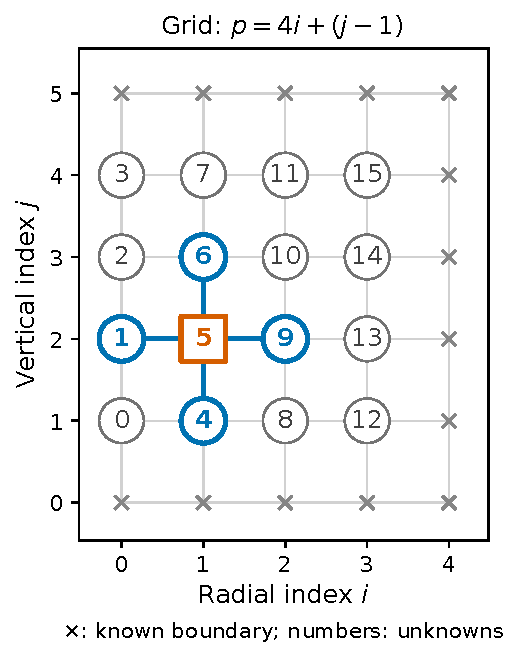
\includegraphics[height=80mm]{appB_grid_numbering.pdf}\\[-1mm]
 {\small (a) Grid numbering}
\end{minipage}\hfill
\begin{minipage}[t]{0.48\linewidth}
 \centering
 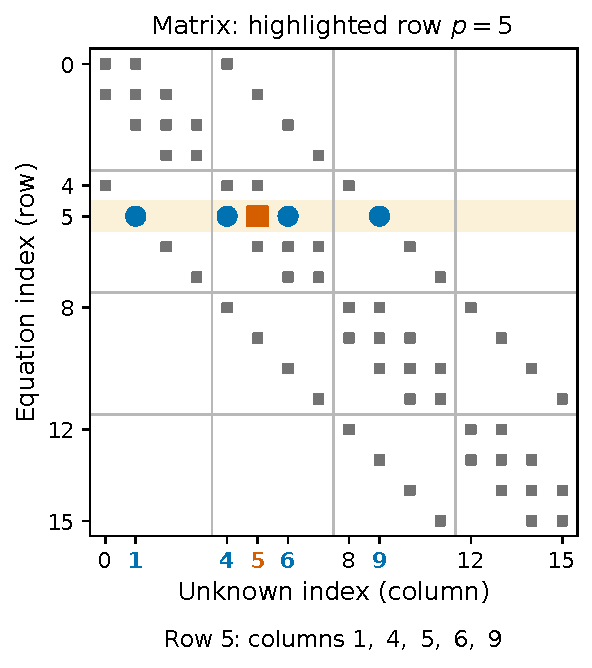
\includegraphics[height=80mm]{appB_sparse_pattern.pdf}\\[-1mm]
 {\small (b) Nonzero matrix entries}
\end{minipage}
\caption{小さい格子と疎行列の対応。説明用に $N_R=4$, $N_Z=5$（$n_z=4$、未知数16個）とした。左図の数字は未知数番号 $p$、$\times$ は既知の境界点である。赤い四角で示す $(i,j)=(1,2)$ は $p=5$ に対応し、青い丸の近傍点を含めた5点は、右図の行番号5（0始まり）の列番号 $1,4,5,6,9$ に対応する。右図の空白は零要素、灰色はその他の非零要素である。}
\label{fig:appB-sparse-pattern}
\end{figure}

番号が隣り合っていても、格子上で隣り合うとは限らない。
例えば、この図の $p=3$ と $p=4$ は動径点の切り替わりに当たり、$z$ 方向の近傍点ではない。
係数を入れる前に $(i,j)$ の範囲で境界を判定するのは、このような誤った結合を避けるためでもある。

\begin{cautionblock}{行列の記憶量と求解の計算量を分ける}
密行列の要素数は未知数の2乗で増えるが、ここで組み立てる疎行列の非零要素数は未知数にほぼ比例する。
ただし、これだけで求解の計算時間も比例すると結論することはできない。
疎行列の直接法ではフィルインも生じるため、分解中の記憶量と計算量は元の非零要素数だけでは決まらない。
\end{cautionblock}

\begin{topicblock}{シミュレーション天文学で使う重力計算法}
本付録では、Poisson 方程式を有限差分で離散化し、疎行列の連立一次方程式を解いた。
これは境界値問題の設定から数値解の検証までを学ぶための一例であり、すべての重力計算で同じ手順を使うわけではない。

\begin{itemize}
\item \textbf{滑らかな固定重力場：}
複雑な質量分布の重力場には、角度依存性を球面調和関数で表す\textbf{多重極展開（multipole expansion）}や、
密度とポテンシャルを対応する基底関数の和で表す\textbf{基底関数展開法（basis-function expansion）}などを使える。
あらかじめ構成した展開式や補間関数を微分すれば、任意の位置で加速度を評価できる。
固定場での軌道積分中に、空間上の Poisson 方程式を解き直す必要はない。
多重極展開は、第2章で紹介した遠方の境界値だけでなく、質量分布の内部の重力場を表すことにも用いられる。

\item \textbf{格子上の自己重力計算：}
一様格子では、\textbf{高速 Fourier 変換（fast Fourier transform; FFT）}を利用して
Poisson 方程式を解く方法があり、周期境界条件と組み合わせやすい。
粗い格子と細かい格子を組み合わせて離散方程式を解く\textbf{多重格子法（multigrid method）}は、
適合格子細分化法（adaptive mesh refinement; AMR）を用いる計算でも利用される。
有限差分法は方程式の\textbf{離散化}、多重格子法は離散方程式の\textbf{求解}の方法であり、
両者は組み合わせて使える。FFT も有限差分法と対立するものではなく、
有限差分で得た離散方程式を解くために利用する場合がある。

\item \textbf{粒子分布からの重力計算：}
\textbf{ツリー法（tree method）}では、遠方の粒子群からの重力を、多重極展開を使ってまとめて近似する。
\textbf{PM 法（particle-mesh method）}では、粒子の質量を格子へ割り当て、
格子上でポテンシャルと加速度を求め、加速度を粒子位置へ補間する。
格子上のポテンシャルを差分して加速度を求める実装もあり、PM 法も有限差分法と排他的な方法ではない。
重力を長距離成分と短距離成分に分け、前者を PM 法、後者をツリー法で計算する TreePM 法もある。
\end{itemize}

以上は用途に沿った例であり、排他的な分類ではない。基底関数展開を自己重力系の時間発展に用いることもできる。
研究では質量分布、境界条件、必要な空間分解能、計算規模に応じて方法を選ぶ。
方法が変わっても、参照解との比較や、格子幅・展開の項数などの近似の細かさを変えた検証は必要である。
詳しくは Binney \& Tremaine（2008）の§2.4・§2.8・§2.9\cite{bt2008}、松本ほか\cite{matsumoto}、富阪ほか編\cite{tomisaka2007}を参照すること。
\end{topicblock}

\section{数値解と誤差}
\label{sec:appB-poisson-results}

Notebook B の \texttt{solve\_mn\_poisson} は、ここまでの格子作成、係数行列と右辺の構成、求解、2次元配列への復元を一つにまとめた関数である。
同じ格子点で数値解と解析解を評価し、ポテンシャルの誤差と離散方程式の残差を別々に求める。

\begin{notebookblock}{B｜2次元 Poisson 方程式の数値解}
式\eqref{eq:appB-main-grid}の領域と区間数で解く。
\texttt{Phi\_num[i,j]} に合わせ、\texttt{meshgrid} の \texttt{indexing="ij"} によって解析解の配列も第1軸を $R$、第2軸を $z$ にする。

{\sffamily\small\color{graytext}対応セル（計算部分）}
\begin{Verbatim}[fontsize=\small,xleftmargin=2mm,frame=single,framesep=1.8mm,framerule=0.35pt,rulecolor=\color{listingframe},fillcolor=\color{listingbg}]
# 計算領域と各方向の区間数を指定する
NR, NZ = 40, 64
Rmax = 5.0 * amn
Zmax = 4.0 * amn
Rmn, zmn, Phi_num, A_mn, rhs_mn, sol_mn = solve_mn_poisson(
    NR=NR, NZ=NZ, Rmax=Rmax, Zmax=Zmax, G=G, M=Mmn, a=amn, b=bmn)

# 数値解と同じ格子上で解析ポテンシャルを評価する
RRmn, ZZmn = np.meshgrid(Rmn, zmn, indexing="ij")
Phi_exact_mn = phi_mn(RRmn, ZZmn, G, Mmn, amn, bmn)

# 解の誤差と、離散方程式の残差を別々に測る
err_phi = np.max(np.abs(Phi_num - Phi_exact_mn)) / (G * Mmn / amn)
residual = A_mn @ sol_mn - rhs_mn
residual_max = np.max(np.abs(residual))
\end{Verbatim}
\end{notebookblock}

ここで用いる誤差は、全格子点での絶対誤差の最大値を、一定の基準量 $GM/a$ で割った
\begin{equation}
 \epsilon_\Phi=\frac{\max_{i,j}|\Phi_{{\rm num},i,j}-\Phi_{{\rm exact},i,j}|}{GM/a}=\appBPhiError
\label{eq:appB-poisson-error}
\end{equation}
である。各点の $|\Phi_{\rm exact}|$ で割った相対誤差ではない。
境界には解析値を設定しているため、境界点での差は0になる。
数値ポテンシャルを図\ref{fig:appB-mn-potential}、符号付きの誤差を図\ref{fig:appB-mn-error}に示す。

\begin{figure}[!htbp]
\centering
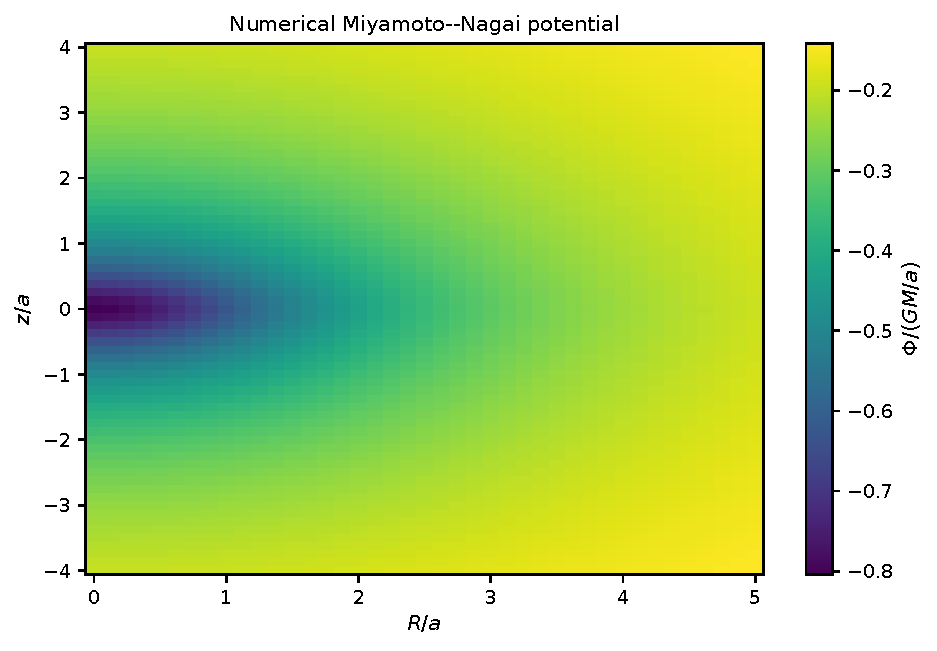
\includegraphics[width=0.64\linewidth]{appB_mn_potential.pdf}
\caption{有限差分法で求めた Miyamoto--Nagai ポテンシャル。$N_R=40$, $N_Z=64$ とし、$R=R_{\max}$ と $z=\pm Z_{\max}$ には解析値を与えた。対称軸の値は差分方程式を解いて求めている。}
\label{fig:appB-mn-potential}
\end{figure}

\begin{figure}[!htbp]
\centering
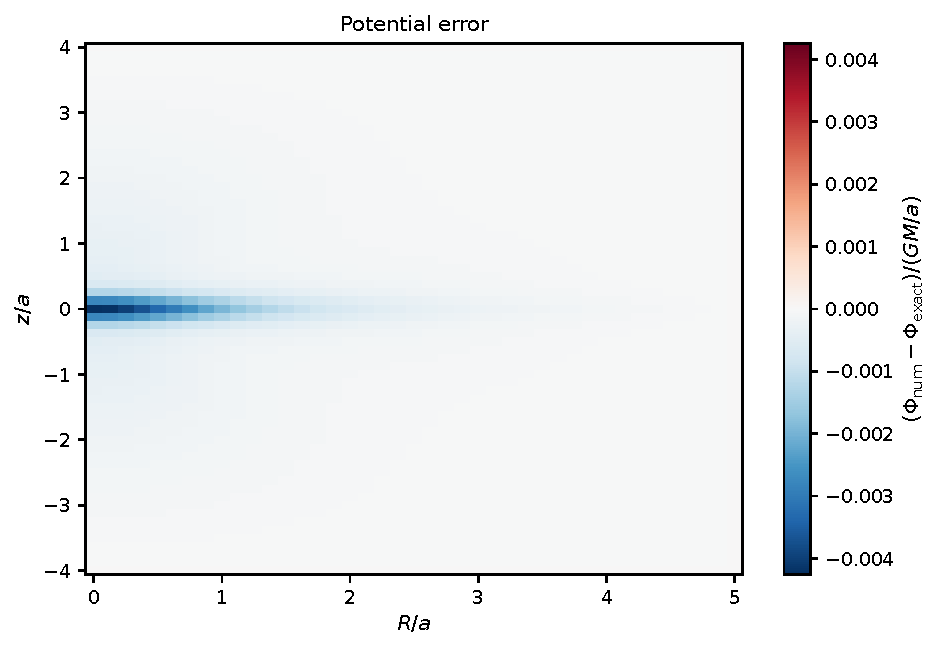
\includegraphics[width=0.64\linewidth]{appB_mn_error.pdf}
\caption{同じ格子上の数値解と解析解の差を $GM/a$ で規格化したもの。符号付き誤差を、0を中心とする対称なカラースケールで表示している。境界点での差は0である。}
\label{fig:appB-mn-error}
\end{figure}

一方、未知点の解ベクトルについて計算した最大残差は
\begin{equation}
 \max_p|(A\boldsymbol{\Phi}-\boldsymbol{b})_p|=\appBResidual
\label{eq:appB-residual}
\end{equation}
である。
これは、上で定義した差分係数を使い、$G=M=a=1$ で計算した値である。
残差は離散方程式の左右のずれであり、ポテンシャルの誤差とは単位も異なる。
方程式全体を定数倍すれば残差も定数倍されるため、異なる規格化の残差をそのまま比較しない。

\begin{cautionblock}{残差が小さくても離散化誤差は残る}
第2章の残差の定義と同じく、ここで小さい残差が示すのは、数値解が組み立てた連立一次方程式をよく満たすことである。
その方程式は連続な Poisson 方程式そのものではないため、解析解との差は残る。
ポテンシャルの精度は、式\eqref{eq:appB-poisson-error}と格子収束試験で別に確認する。
\end{cautionblock}

\section{2次元 Poisson 方程式の格子収束}
\label{sec:appB-poisson-convergence}

一つの格子で解と残差を確認した後は、領域・境界条件・モデルを固定して格子を細かくする。
内部点と対称軸で使った差分は、滑らかな解に対して各方向で2次精度である。
二つの格子幅を一定の比率で小さくすれば、離散化誤差が支配する十分細かい格子で
\begin{equation}
 \epsilon_\Phi\propto h^2,\qquad h\equiv\max(\Delta R,\Delta z)
\label{eq:appB-poisson-conv-expected}
\end{equation}
が期待される。
ただし、第2章で述べたように、差分公式の打ち切り誤差の次数だけで数値解全体の収束が保証されるわけではない。
ここでも、境界を含むソルバー全体の結果から次数を測定する。

\medskip
\noindent\textbf{検証手順｜2次元格子の収束試験}
\par\smallskip
\begin{enumerate}[itemsep=0em,topsep=0.1em]
\item $R_{\max}=5a$, $Z_{\max}=4a$、モデルのパラメータ、解析的な境界条件を固定する。
\item $N_R$ と $N_Z$ を同じ比率で増やし、両方向の格子幅を小さくする。
\item 各格子の数値解を同じ格子上の解析解と比較し、$\epsilon_\Phi$ を計算する。
\item 両対数表示の傾きから収束次数を測定し、期待する2次収束と比較する。
\end{enumerate}

Notebook B では $(N_R,N_Z)=(40,64),(60,96),(80,128),(100,160)$ とする。
この組では常に $\Delta R=\Delta z$ であり、$h/a$ は $0.125,0.08333\ldots,0.0625,0.05$ となる。
$R$ 方向だけを細かくして $\Delta z$ を固定する比較とは異なる。

\begin{notebookblock}{B｜2次元 Poisson 方程式の格子収束}
各格子で得た $\epsilon_\Phi$ と $h$ を配列に保存する。
\texttt{polyfit} では、この4格子の両対数データに直線を当てはめ、その傾きを収束次数とする。

{\sffamily\small\color{graytext}対応セル（計算部分）}
\begin{Verbatim}[fontsize=\small,xleftmargin=2mm,frame=single,framesep=1.8mm,framerule=0.35pt,rulecolor=\color{listingframe},fillcolor=\color{listingbg}]
# 領域とモデルを固定し、両方向の区間数を同じ比率で増やす
grid_list = [(40, 64), (60, 96), (80, 128), (100, 160)]
h_list = []
err_list = []

for NR_i, NZ_i in grid_list:
    R_i, z_i, Phi_i, _, _, _ = solve_mn_poisson(
        NR=NR_i, NZ=NZ_i, Rmax=Rmax, Zmax=Zmax,
        G=G, M=Mmn, a=amn, b=bmn)

    # 同じ格子上の解析解から、規格化した最大絶対誤差を測る
    RR_i, ZZ_i = np.meshgrid(R_i, z_i, indexing="ij")
    Phi_ex_i = phi_mn(RR_i, ZZ_i, G, Mmn, amn, bmn)
    h_i = max(R_i[1] - R_i[0], z_i[1] - z_i[0])
    err_i = np.max(np.abs(Phi_i - Phi_ex_i)) / (G * Mmn / amn)
    h_list.append(h_i)
    err_list.append(err_i)

h_list = np.array(h_list)
err_list = np.array(err_list)

# epsilon_Phi が h^p に比例する範囲では、両対数の傾きが p
order_2d = np.polyfit(np.log(h_list), np.log(err_list), 1)[0]
\end{Verbatim}
\end{notebookblock}

この4格子から得られる次数は
\begin{equation}
 p=\appBOrderTwoD
\label{eq:appB-poisson-conv-measured}
\end{equation}
であり、図\ref{fig:appB-poisson-convergence}のように誤差はほぼ2次で減少する。
これは、ここで用いた滑らかなモデル、解析的な境界条件、格子幅の範囲に対する実測値である。
別の密度分布や境界条件へ変更する場合も、同じ検証を繰り返す必要がある。

\begin{figure}[!htbp]
\centering
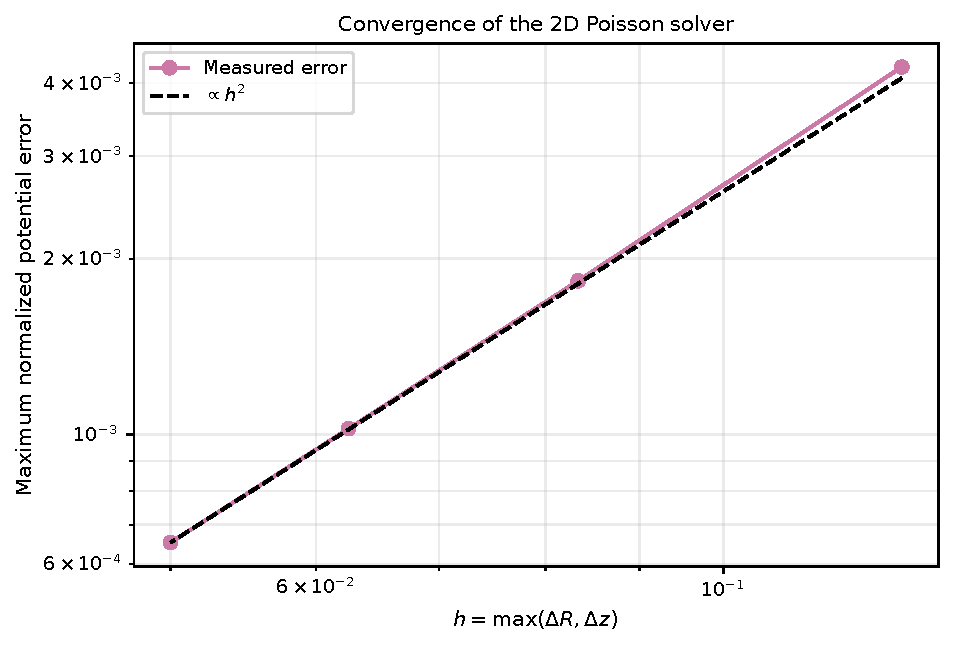
\includegraphics[width=0.64\linewidth]{appB_poisson2d_convergence.pdf}
\caption{領域と境界条件を固定した2次元 Poisson 方程式の格子収束。実線は規格化した最大絶対誤差、破線は最も細かい格子の誤差に合わせた $h^2$ の比較線である。4格子から測定した収束次数は $p=\appBOrderTwoD$ となる。}
\label{fig:appB-poisson-convergence}
\end{figure}

\chapter{軸対称・非軸対称ポテンシャル中の軌道}
\label{app:orbit-applications}

第3章では、球対称な重力場の中で軌道を計算し、時間積分法を検証した。
本付録では、加速度関数を差し替えて同じ積分法を再利用する。
ただし、重力場を変えると、検証に使える保存量や比較の基準も変わる。
Ryden §7.2--7.3\cite{ryden2025}の軸対称・非軸対称ポテンシャルを題材として、数値軌道と近似解の比較、時間刻みを変えた収束試験、保存量による診断を学ぶ。
本付録は第3章の発展であり、他の付録を先に読む必要はない。

\begin{learningbox}[本付録で学ぶこと]
\begin{itemize}
 \item 加速度関数と初期条件を設定し、第3章の時間積分法を異なる重力場へ再利用できる。
 \item ポテンシャルの対称性に応じて保存量を選び、数値軌道の診断に用いることができる。
 \item 厳密解が得られない問題で、小振幅近似を近似的な参照解として用い、数値軌道との差を評価できる。
 \item 時間刻みと初期振幅を別々に変え、時間積分の誤差と小振幅近似との差を区別できる。
 \item 非軸対称系の角運動量の変化を数値誤差と区別し、有限時間の軌道から判断できる範囲を説明できる。
\end{itemize}
\end{learningbox}

数値実験は Notebook C で行う。積分関数は第3章のものを使い、本文では加速度の実装と検証方法を中心に説明する。

\section{異なる重力場への時間積分法の適用}
\label{sec:appC-reuse}

本付録のポテンシャルは時間に依存せず、計算する粒子の運動によっても変わらないものとする。
重力加速度 $\boldsymbol g(\boldsymbol x)=-\nabla\Phi$ は位置だけで決まるため、第3章のキック--ドリフト--キック（KDK）形式のリープフロッグ法をそのまま使える。
\texttt{acc\_func(x)} は1点の位置配列を受け取り、同じ次元の加速度配列を返す関数である。
積分器と重力場の計算を分けておけば、モデルごとに時間ループを書き直す必要はない。

円筒座標を $(R,\phi,z)$ とし、$R=\sqrt{x^2+y^2}$、$\phi$ は方位角、$z$ は対称軸方向の座標とする。
ポテンシャルを $R,z$ で表す場合も、Notebook C では Cartesian 座標の位置と速度を更新する。
返される配列の形は \texttt{(nstep + 1, ndim)} で、初期状態を含む。
半径や保存量は、この配列から各出力時刻で計算する。

第3章と同様に、比エネルギーと比角運動量の $z$ 成分を
\begin{equation}
 E=\frac12|\boldsymbol v|^2+\Phi(\boldsymbol x),\qquad
 L_z=xv_y-yv_x
\label{eq:appC-diagnostics}
\end{equation}
とする。
時間に依存しないポテンシャルでは $E$ が保存する。
また、$dL_z/dt=xg_y-yg_x$ は $z$ 軸まわりのトルクなので、軸対称な力では0となり、$L_z$ も保存する。
したがって、数値的な $E$ や $L_z$ の変化を誤差とみなせるかどうかは、モデルの対称性に応じて判断する必要がある。
以下では第3章と同様に、文脈が明らかな場合はこれらを単にエネルギー、角運動量と呼ぶ。

以下では解析的な加速度を用い、付録\ref{app:axisym-poisson}の数値 Poisson 解は入力しない。
これにより、空間離散化や補間の誤差を混ぜずに、時間積分を検証する。

\section{軸対称ポテンシャルとエピサイクル運動}
\label{sec:appC-axisymmetric}

\subsection{対数ポテンシャルと加速度の実装}

平坦な回転曲線を持つ対数ポテンシャル（logarithmic potential）
\begin{equation}
 \Phi(R,z)=\frac12v_0^2\ln\left(\frac{R^2+z^2/q^2}{\ell^2}\right)
\label{eq:appC-log-axisym}
\end{equation}
を用いる。
$v_0>0$ は速度のスケール、$q>0$ は等ポテンシャル面の形を決める定数であり、$q<1$ では扁平な形になる。
$\ell$ は対数の引数を無次元にする固定の基準長さで、以下のコードでは $\ell=1$ とする。
この選択はポテンシャルの加法定数を定めるだけで、加速度には影響しない。
原点ではポテンシャルと加速度が特異になるため、ここでは原点を通らない、ほぼ円軌道を扱う。

$R^2=x^2+y^2$ を代入して
\begin{equation}
 D=x^2+y^2+\frac{z^2}{q^2}
\end{equation}
と置く。
例えば $\partial D/\partial x=2x$、$\partial D/\partial z=2z/q^2$ なので、
\begin{equation}
 g_x=-\frac{v_0^2x}{D},\qquad
 g_y=-\frac{v_0^2y}{D},\qquad
 g_z=-\frac{v_0^2z}{q^2D}
\label{eq:appC-log-acceleration}
\end{equation}
となる。
この3成分を1つの配列で返す関数が Listing C.1 である。
引数 \texttt{x} は3成分の位置配列であり、式中のスカラー $x$ とは区別する。

\begin{listingbox}{C.1　対数ポテンシャルの加速度}
\begin{Verbatim}[fontsize=\small,xleftmargin=1mm]
def acc_log_axisym(x, v0=1.0, q=0.8):
    # ポテンシャルの勾配を Cartesian 座標で評価する。
    x = np.asarray(x)
    den = x[0]**2 + x[1]**2 + x[2]**2 / q**2
    return -v0**2 * np.array([x[0], x[1], x[2] / q**2]) / den
\end{Verbatim}
\end{listingbox}


\subsection{半径方向のエピサイクル振動数}

円軌道のまわりの小さな振動を、エピサイクル運動（epicyclic motion）として近似する。
Ryden は $z$ 方向の比角運動量を $j_z$ と書くが、本書では $L_z$ と表す。
軸対称性によって
\begin{equation}
 L_z=R^2\dot\phi=\mathrm{const.}
\label{eq:appC-jz}
\end{equation}
なので、半径・鉛直方向の運動は有効ポテンシャル（effective potential）
\begin{equation}
 \Phi_{\rm eff}(R,z)=\Phi(R,z)+\frac{L_z^2}{2R^2}
\label{eq:appC-effective-potential}
\end{equation}
で記述できる。これは Ryden 式(7.35) に対応する\cite{ryden2025}。
半径方向の運動方程式は $\ddot R=-\partial\Phi_{\rm eff}/\partial R$ である。

円軌道の案内中心半径（guiding radius）を $R_g>0$ とする。
$z=0$ では $\Phi(R,0)=v_0^2\ln(R/\ell)$ であるから、円軌道の条件は
\begin{equation}
 \left.\frac{\partial\Phi_{\rm eff}}{\partial R}\right|_{(R_g,0)}
 =\frac{v_0^2}{R_g}-\frac{L_z^2}{R_g^3}=0
\end{equation}
となる。以下では正の向きに回る円軌道を選ぶ。比角運動量と角速度は次式で与えられる。
\begin{equation}
 L_z=R_gv_0,\qquad \Omega=\frac{v_0}{R_g}
\label{eq:appC-jz-circular}
\end{equation}

半径方向の変位を $\xi=R-R_g$ と書く。
有効ポテンシャルを $\xi$ の2次まで Taylor 展開すると、円軌道の条件によって1次の項が消え、
\begin{equation}
 \Phi_{\rm eff}(R,0)\simeq\Phi_{\rm eff}(R_g,0)+\frac12\kappa^2\xi^2
\end{equation}
となる。係数は
\begin{align}
 \kappa^2
 &=\left.\frac{\partial^2\Phi_{\rm eff}}{\partial R^2}\right|_{(R_g,0)}
 =-\frac{v_0^2}{R_g^2}+\frac{3L_z^2}{R_g^4}
 =\frac{2v_0^2}{R_g^2}
\end{align}
である。
したがって、線形化した運動方程式は $\ddot\xi=-\kappa^2\xi$ となり、
\begin{equation}
 \boxed{\kappa=\sqrt{2}\,\Omega}
\label{eq:appC-kappa}
\end{equation}
を得る。初期変位を $\xi_0$、初期半径速度を0とすると、
\begin{equation}
 R(t)-R_g\simeq\xi_0\cos(\kappa t)
\label{eq:appC-radial-harmonic}
\end{equation}
が比較に用いる近似解である。

\subsection{鉛直振動数}

$z=0$ のまわりでも Taylor 展開を行う。
ポテンシャルは $z$ の偶関数なので1次の項はなく、$R=R_g$ で
\begin{equation}
 \Phi(R_g,z)\simeq\Phi(R_g,0)+\frac12\nu_z^2z^2
\end{equation}
となる。
$\partial\Phi/\partial z=v_0^2z/[q^2(R^2+z^2/q^2)]$ をさらに微分して $z=0$ と置くと、
\begin{equation}
 \nu_z^2=\left.\frac{\partial^2\Phi}{\partial z^2}\right|_{(R_g,0)}
 =\frac{v_0^2}{q^2R_g^2},\qquad
 \boxed{\nu_z=\frac{v_0}{qR_g}}
\label{eq:appC-nuz}
\end{equation}
を得る。これは Ryden 式(7.47) を対数ポテンシャルに適用したものである\cite{ryden2025}。
初期鉛直速度も0とすると、
\begin{equation}
 z(t)\simeq z_0\cos(\nu_z t)
\label{eq:appC-vertical-harmonic}
\end{equation}
となる。
この近似では $|\xi|/R_g\ll1$、$|z|/(qR_g)\ll1$ とし、半径方向と鉛直方向の結合を高次の項として省いている。
式\eqref{eq:appC-radial-harmonic}と式\eqref{eq:appC-vertical-harmonic}は、元の運動方程式の厳密解ではない。

\subsection{初期条件と数値軌道の比較}

Notebook C では $v_0=1$、$q=0.8$、$R_g=1$ とし、
\begin{equation}
 \Omega=\appCOmegaAxisym,\qquad
 \kappa=\appCKappaAxisym,\qquad
 \nu_z=\appCNuAxisym
\end{equation}
を用いる。
初期変位を $\xi_0=z_0=0.05R_g$ とし、
\begin{equation}
 \boldsymbol x_{\rm init}=(R_g+\xi_0,0,z_0),\qquad
 \boldsymbol v_{\rm init}=\left(0,\frac{R_gv_0}{R_g+\xi_0},0\right)
\label{eq:appC-axisym-initial}
\end{equation}
とする。
初期半径をずらしても、方位角方向の速度をこのように選べば $L_z=R_gv_0$ を保てる。
基準周期 $T_\phi=2\pi/\Omega$ に対して、$\Delta t=T_\phi/300$ で $12T_\phi$ まで積分する。
$T_\phi$ は案内中心の円軌道の周期であり、数値軌道の実測周期ではない。

\begin{notebookblock}{C｜ほぼ円軌道とエピサイクル運動}
\texttt{x\_amp} が $\xi_0$、\texttt{z\_amp} が $z_0$ に対応する。
近似解と数値軌道に同じ初期変位を用い、比較する時刻も揃える。
加速度関数と初期条件を積分器へ渡す部分は、モデルを変えても共通である。
\par\smallskip\noindent\begin{minipage}{\linewidth}
{\sffamily\small\color{graytext}対応セル（初期条件と基準周期）}
\begin{Verbatim}[fontsize=\footnotesize,xleftmargin=2mm,frame=single,framesep=1.8mm,framerule=0.35pt,rulecolor=\color{listingframe},fillcolor=\color{listingbg}]
# 案内中心からの初期変位と、保つべき比角運動量を設定する。
Rg = 1.0
x_amp = 0.05 * Rg
z_amp = 0.05 * Rg
Lz_circ = Rg * vlog
R_init = Rg + x_amp
vphi_init = Lz_circ / R_init
x0_ax = np.array([R_init, 0.0, z_amp])
v0_ax = np.array([0.0, vphi_init, 0.0])

# 近似解の振動数と、案内中心の円軌道の周期を求める。
Omega = vlog / Rg
kappa = np.sqrt(2.0) * Omega
nu_z = vlog / (qlog * Rg)
Tphi = 2.0 * np.pi / Omega
\end{Verbatim}
\end{minipage}

\par\smallskip\noindent\begin{minipage}{\linewidth}
{\sffamily\small\color{graytext}対応セル（時間積分と診断量）}
\begin{Verbatim}[fontsize=\footnotesize,xleftmargin=2mm,frame=single,framesep=1.8mm,framerule=0.35pt,rulecolor=\color{listingframe},fillcolor=\color{listingbg}]
# 同じ加速度関数を各時間ステップで使い、12Tphiまで積分する。
dt_ax = Tphi / 300.0
nstep_ax = int(round(12.0 * Tphi / dt_ax))
t_ax = np.arange(nstep_ax + 1) * dt_ax
acc_ax = lambda x: acc_log_axisym(x, vlog, qlog)
x_ax, v_ax = integrate_leapfrog(acc_ax, x0_ax, v0_ax, dt_ax, nstep_ax)

# 各時刻の半径と、保存量の診断に用いる配列を求める。
R_ax = np.sqrt(x_ax[:, 0]**2 + x_ax[:, 1]**2)
E_ax = energy_log_axisym(x_ax, v_ax, vlog, qlog)
Lz_ax = Lz_3d(x_ax, v_ax)
\end{Verbatim}
\end{minipage}

\end{notebookblock}

図\ref{fig:appC-radial-epicycle}と図\ref{fig:appC-vertical}では、最初の $3T_\phi$ の数値軌道と近似解を比較している。
両者はほぼ同じ振動を示すが、有限の初期振幅では完全には一致しない。
この差の解釈には、後述の時間刻みと初期振幅を変える検証が必要になる。

\begin{figure}[!htbp]
\centering
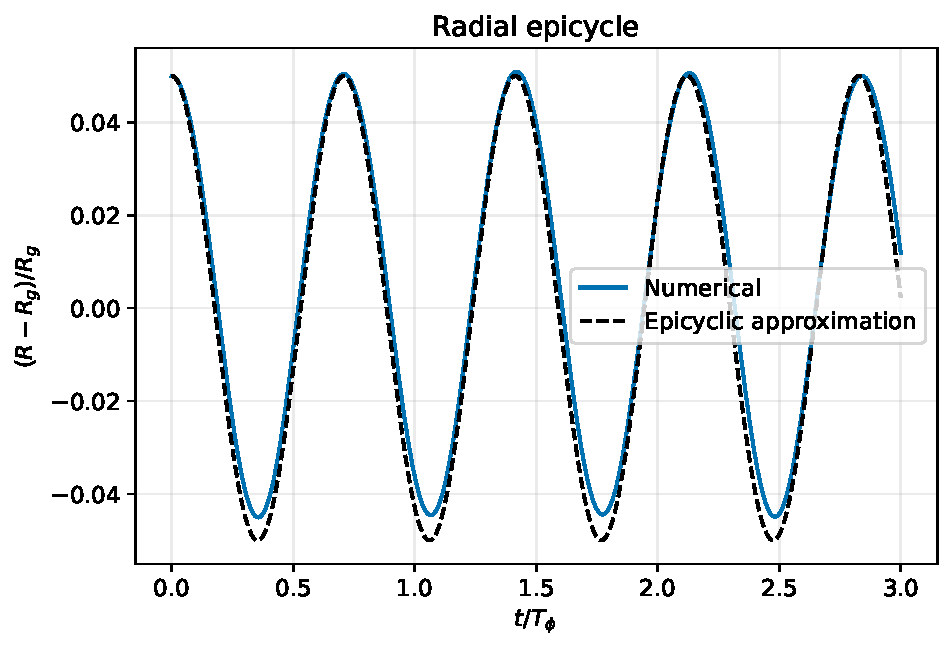
\includegraphics[width=0.64\linewidth]{appC_radial_epicycle.pdf}
\caption{数値軌道の半径方向変位と、小振幅近似 $\xi_0\cos(\kappa t)$ の比較。初期変位と初期半径速度を揃え、同じ時刻で評価している。}
\label{fig:appC-radial-epicycle}
\end{figure}

\begin{figure}[!htbp]
\centering
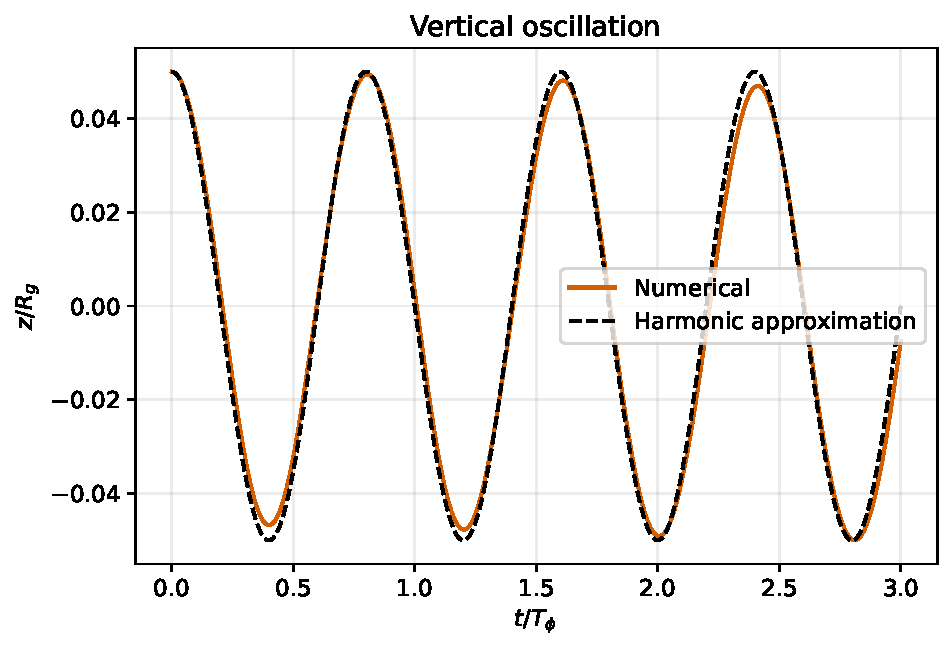
\includegraphics[width=0.64\linewidth]{appC_vertical_oscillation.pdf}
\caption{数値軌道の鉛直変位と、小振幅近似 $z_0\cos(\nu_z t)$ の比較。半径・鉛直方向の結合は近似解に含まれていない。}
\label{fig:appC-vertical}
\end{figure}

保存量の診断には、初期値を $E_0=E(0)$、$L_{z,0}=L_z(0)$ として、
\begin{equation}
 \epsilon_E=\frac{\max_n|E(t_n)-E_0|}{|E_0|},\qquad
 \epsilon_{L_z}=\frac{\max_n|L_z(t_n)-L_{z,0}|}{|L_{z,0}|}
\label{eq:appC-invariant-errors}
\end{equation}
を用いる。この例では両分母は0ではなく、$0\le t\le12T_\phi$ の全出力時刻で測ると、
\begin{equation}
 \epsilon_E=\appCAxisymMaxEnergy,\qquad
 \epsilon_{L_z}=\appCAxisymMaxLz
\end{equation}
となる。
軸対称な力ではキックによる $L_z$ の変化が0であり、ドリフトも角運動量を変えない。
このため、リープフロッグ法は $L_z$ を丸め誤差の範囲で保つ。
第3章§\ref{sec:ch3-invariants}の球対称系では角運動量ベクトル全体について成り立った性質が、ここでは $z$ 成分について成り立つ。
ただし、$L_z$ がよく保たれていても、各時刻の位置の精度は別に確認する必要がある。

\begin{cautionblock}{エネルギーの基準と相対誤差}
ポテンシャルの加法定数を変えると、軌道は同じでも $E_0$ が変わる。
エネルギーの相対誤差を比較するときは、その基準を固定する。
$E_0=0$ または $L_{z,0}=0$ の場合には式\eqref{eq:appC-invariant-errors}は使わず、絶対的な変化や、別に定めた非零のスケールで規格化した変化を用いる。
\end{cautionblock}

\subsection{時間刻みと初期振幅を変えた検証}

第3章の円軌道では厳密解との位置の差を時間積分誤差として測った。
一方、ここで用いた小振幅近似との差には、時間積分の誤差と、線形化で省いた項の影響が含まれる。
そこで、まず初期振幅と終端時刻を固定し、時間刻み $\Delta t$ と $\Delta t/2$ の数値軌道どうしを比較する。

共通する出力時刻で位置の最大差を
\begin{equation}
 D_{\Delta t}=\max_{t_n}\frac{|\boldsymbol x_{\Delta t}(t_n)-\boldsymbol x_{\Delta t/2}(t_n)|}{R_g}
\label{eq:appC-self-difference}
\end{equation}
と定める。
離散化誤差が支配する範囲で、同じ時刻の数値解が
$\boldsymbol x_{\Delta t}=\boldsymbol x_{\rm exact}+\boldsymbol C(\Delta t)^p+\cdots$
と書ければ、差の主要項は $\boldsymbol C(1-2^{-p})(\Delta t)^p$ となる。
このため、
\begin{equation}
 p_{\rm self}=\log_2\frac{D_{\Delta t}}{D_{\Delta t/2}}
\label{eq:appC-self-order}
\end{equation}
から収束次数を推定できる。
$D_{\Delta t}$ は2つの数値解の差であり、厳密解に対する誤差そのものではない。
また、共通の実装上の誤りがあっても数値解どうしは収束し得るため、加速度の式や保存量の確認も併用する。

Listing C.2 は式\eqref{eq:appC-self-difference}の計算部分である。
細かい時間刻みの配列から \texttt{[::2]} で1点おきに取り出すと、粗い配列の時刻と一致する。
\texttt{axis=1} は各時刻の位置ベクトルの大きさを求める指定である。

\begin{listingbox}{C.2　共通する時刻での位置の差と収束次数}
\begin{Verbatim}[fontsize=\small,xleftmargin=1mm]
self_diffs = []
for x_coarse, x_fine in zip(trial_orbits[:-1], trial_orbits[1:]):
    dx = x_coarse - x_fine[::2]
    self_diffs.append(np.max(np.linalg.norm(dx, axis=1)) / Rg)
self_diffs = np.asarray(self_diffs)
p_self = np.log2(self_diffs[:-1] / self_diffs[1:])
\end{Verbatim}
\end{listingbox}


Notebook C では $\xi_0=z_0=0.05R_g$、終端時刻 $3T_\phi$ を固定し、1基準周期あたり300、600、1200、2400ステップで積分する。
結果を表\ref{tab:appC-self-convergence}に示す。刻みを半分にすると差は約4分の1になり、リープフロッグ法の2次収束と整合する。

\begin{table}[!htbp]
\centering
\caption{同じ初期条件・終端時刻で得た数値軌道どうしの比較。最後の行は $D_{\Delta t/2}$ に必要な、さらに細かい計算を行っていないため、次数を表示しない。}
\label{tab:appC-self-convergence}
\begin{tabular}{ccc}
\toprule
$\Delta t/T_\phi$ & $D_{\Delta t}$ & $p_{\rm self}$ \\
\midrule
$1/300$ & $\appCSelfDiffOne$ & $\appCSelfOrderOne$ \\
$1/600$ & $\appCSelfDiffTwo$ & $\appCSelfOrderTwo$ \\
$1/1200$ & $\appCSelfDiffThree$ & --- \\
\bottomrule
\end{tabular}
\end{table}

次に $\Delta t=T_\phi/2400$ と終端時刻 $3T_\phi$ を固定し、初期振幅だけを小さくする。
$\alpha=\xi_0/R_g=z_0/R_g$ とし、近似解との差を
\begin{equation}
 A_R=\frac{\max_n|R(t_n)-R_g-\xi_0\cos(\kappa t_n)|}{|\xi_0|},\qquad
 A_z=\frac{\max_n|z(t_n)-z_0\cos(\nu_z t_n)|}{|z_0|}
\label{eq:appC-amplitude-differences}
\end{equation}
で測る。
初期振幅で規格化するのは、振幅を小さくしたため絶対差が小さくなっただけなのか、振幅に比べても一致が改善したのかを区別するためである。
この比較では $\alpha>0$ とする。

\begin{table}[!htbp]
\centering
\caption{初期振幅を変えた小振幅近似との比較。括弧内は1基準周期あたりのステップ数である。時間刻みを半分にしたときの変化は、初期振幅を半分にしたときの変化に比べて小さい。}
\label{tab:appC-amplitude-comparison}
\begin{tabular}{ccccc}
\toprule
$\alpha$ & $A_R$ (1200) & $A_R$ (2400) & $A_z$ (1200) & $A_z$ (2400) \\
\midrule
$0.0500$ & $\appCAmpRCoarseOne$ & $\appCAmpRFineOne$ & $\appCAmpZCoarseOne$ & $\appCAmpZFineOne$ \\
$0.0250$ & $\appCAmpRCoarseTwo$ & $\appCAmpRFineTwo$ & $\appCAmpZCoarseTwo$ & $\appCAmpZFineTwo$ \\
$0.0125$ & $\appCAmpRCoarseThree$ & $\appCAmpRFineThree$ & $\appCAmpZCoarseThree$ & $\appCAmpZFineThree$ \\
\bottomrule
\end{tabular}
\end{table}

表\ref{tab:appC-amplitude-comparison}には $\Delta t=T_\phi/1200$ の結果も並べた。
この範囲では、時間刻みをさらに小さくしても近似解との差はほとんど変わらない一方、初期振幅を小さくすると規格化した差も減る。
したがって、近似解との不一致の主な原因を、時間積分ではなく小振幅近似に求められる。
振幅をさらに小さくする場合には、固定した時間刻みの誤差が再び効く可能性があるため、刻みの確認も繰り返す。

\begin{notebookblock}{C｜時間刻みと初期振幅の比較}
\texttt{epicycle\_trial} は、振幅比と1基準周期あたりのステップ数を受け取り、$0\le t\le3T_\phi$ の時刻と位置を返す関数である。
関数内では式\eqref{eq:appC-axisym-initial}の初期条件を設定し、同じ積分器を呼ぶ。
関数の完全な定義と出力整形は Notebook に置く。
\par\smallskip\noindent\begin{minipage}{\linewidth}
{\sffamily\small\color{graytext}対応セル（時間刻みを変えた軌道計算）}
\begin{Verbatim}[fontsize=\footnotesize,xleftmargin=2mm,frame=single,framesep=1.8mm,framerule=0.35pt,rulecolor=\color{listingframe},fillcolor=\color{listingbg}]
# 初期振幅を固定し、各時間刻みで独立に積分する。
steps_per_period = np.array([300, 600, 1200, 2400])
trial_orbits = []
for npp in steps_per_period:
    _, x_trial = epicycle_trial(0.05, npp, Rg, vlog, qlog)
    trial_orbits.append(x_trial)
\end{Verbatim}
\end{minipage}

得られた \texttt{trial\_orbits} に Listing C.2 を適用する。
初期振幅を変える比較では、時間刻みを2通りにして、式\eqref{eq:appC-amplitude-differences}を次のように計算する。
\par\smallskip\noindent\begin{minipage}{\linewidth}
{\sffamily\small\color{graytext}対応セル（初期振幅を変えた近似解との比較）}
\begin{Verbatim}[fontsize=\footnotesize,xleftmargin=2mm,frame=single,framesep=1.8mm,framerule=0.35pt,rulecolor=\color{listingframe},fillcolor=\color{listingbg}]
# 振幅を変えた比較を、2つの十分小さい時間刻みで繰り返す。
amp_fractions = np.array([0.05, 0.025, 0.0125])
amp_error_coarse = []
amp_error_fine = []
for amp_fraction in amp_fractions:
    amp = amp_fraction * Rg
    for npp, errors in [(1200, amp_error_coarse), (2400, amp_error_fine)]:
        t_trial, x_trial = epicycle_trial(amp_fraction, npp, Rg, vlog, qlog)
        R_trial = np.sqrt(x_trial[:, 0]**2 + x_trial[:, 1]**2)
        radial_approx = amp * np.cos(kappa * t_trial)
        vertical_approx = amp * np.cos(nu_z * t_trial)
        A_R = np.max(np.abs(R_trial - Rg - radial_approx)) / amp
        A_z = np.max(np.abs(x_trial[:, 2] - vertical_approx)) / amp
        errors.append([A_R, A_z])
amp_error_coarse = np.asarray(amp_error_coarse)
amp_error_fine = np.asarray(amp_error_fine)
\end{Verbatim}
\end{minipage}

\end{notebookblock}

\section{Miyamoto--Nagai ポテンシャル中の軌道}
\label{sec:appC-mn}

\subsection{加速度関数の差し替え}

別の軸対称モデルとして、Miyamoto--Nagai ポテンシャル
\begin{equation}
 \Phi(R,z)=-\frac{GM}{\sqrt{R^2+(a+\sqrt{z^2+b^2})^2}}
\label{eq:appC-mn-potential}
\end{equation}
を用いる。$a$ と $b$ は長さスケールであり、ここでは $G,M,a,b>0$ とする。
$B=\sqrt{z^2+b^2}$、$D=\sqrt{x^2+y^2+(a+B)^2}$ と置くと、
\begin{equation}
 \frac{\partial D}{\partial x}=\frac{x}{D},\qquad
 \frac{\partial B}{\partial z}=\frac{z}{B},\qquad
 \frac{\partial D}{\partial z}=\frac{(a+B)z}{BD}
\end{equation}
である。$\Phi=-GM/D$ を微分して、
\begin{equation}
 g_x=-\frac{GMx}{D^3},\qquad
 g_y=-\frac{GMy}{D^3},\qquad
 g_z=-\frac{GM(a+B)z}{BD^3}
\label{eq:appC-mn-acceleration}
\end{equation}
を得る。
鉛直方向では $B$ も $z$ に依存することに注意する。

\begin{listingbox}{C.3　Miyamoto--Nagai ポテンシャルの加速度}
\begin{Verbatim}[fontsize=\small,xleftmargin=1mm]
def acc_mn_cart(x, G=1.0, M=1.0, a=1.0, b=0.25):
    # BとDの両方のz依存性を含む解析的な加速度。
    X, Y, Z = x
    R2 = X**2 + Y**2
    B = np.sqrt(Z**2 + b**2)
    D = np.sqrt(R2 + (a + B)**2)

    ax = -G * M * X / D**3
    ay = -G * M * Y / D**3
    az = -G * M * (a + B) * Z / (B * D**3)
    return np.array([ax, ay, az])
\end{Verbatim}
\end{listingbox}


Listing C.3 の関数を積分器へ渡せば、前節と同じ更新式で軌道を求められる。
時間に依存しない軸対称系なので、ここでも
\begin{equation}
 E=\mathrm{const.},\qquad L_z=\mathrm{const.}
\label{eq:appC-mn-invariants}
\end{equation}
が検証に使う性質である。

\subsection{初期条件と保存量による診断}

長さ $a$、速度 $v_*=\sqrt{GM/a}$、時間 $t_*=a/v_*$ を用い、
\begin{equation}
 \frac{\boldsymbol x_0}{a}=(3,0,0.5),\qquad
 \frac{\boldsymbol v_0}{v_*}=(0,0.5,0),\qquad
 \Delta t=0.02t_*,\qquad t_{\rm end}=100t_*
\end{equation}
とする。
Notebook C の既定値は $G=M=a=1$、$b=0.25$ であり、このとき $v_*=t_*=1$ である。
初期エネルギーは
\begin{equation}
 E_0=\appCMNEnergyInitial
\end{equation}
となる。
式\eqref{eq:appC-invariant-errors}で全出力時刻の最大絶対相対変化を測ると、
\begin{equation}
 \epsilon_E=\appCMNMaxEnergy,\qquad
 \epsilon_{L_z}=\appCMNMaxLz
\end{equation}
である。
図\ref{fig:appC-mn-orbit}の軌道の形と合わせてこれらを確認する。
$L_z$ が丸め誤差の範囲で保たれることは、前節と同じキックとドリフトの性質による。
位置の精度は、初期条件と終端時刻を固定した時間刻みの収束試験で別に調べる。

\begin{notebookblock}{C｜Miyamoto--Nagai 軌道}
モデルのパラメータを変えても、初期条件と時間の単位が対応するように設定する。
数値 Poisson 解は入力せず、解析的な加速度を使う。
\par\smallskip\noindent\begin{minipage}{\linewidth}
{\sffamily\small\color{graytext}対応セル（単位・初期条件の設定、積分、診断量）}
\begin{Verbatim}[fontsize=\footnotesize,xleftmargin=2mm,frame=single,framesep=1.8mm,framerule=0.35pt,rulecolor=\color{listingframe},fillcolor=\color{listingbg}]
# モデルを設定し、長さ・速度・時間の単位を揃える。
M_mn, a_mn, b_mn = 1.0, 1.0, 0.25
vscale_mn = np.sqrt(G * M_mn / a_mn)
tscale_mn = a_mn / vscale_mn
x0_mn = a_mn * np.array([3.0, 0.0, 0.5])
v0_mn = vscale_mn * np.array([0.0, 0.5, 0.0])

# 解析的な加速度で100時間単位まで積分する。
dt_mn = 0.02 * tscale_mn
nstep_mn = int(round(100.0 * tscale_mn / dt_mn))
t_mn = np.arange(nstep_mn + 1) * dt_mn
acc_mn = lambda x: acc_mn_cart(x, G, M_mn, a_mn, b_mn)
x_mn, v_mn = integrate_leapfrog(acc_mn, x0_mn, v0_mn, dt_mn, nstep_mn)

# 位置・速度から半径と保存量を計算する。
E_mn = energy_mn(x_mn, v_mn, G, M_mn, a_mn, b_mn)
Lz_mn = Lz_3d(x_mn, v_mn)
R_mn = np.sqrt(x_mn[:, 0]**2 + x_mn[:, 1]**2)
\end{Verbatim}
\end{minipage}

\end{notebookblock}

\begin{figure}[!htbp]
\centering
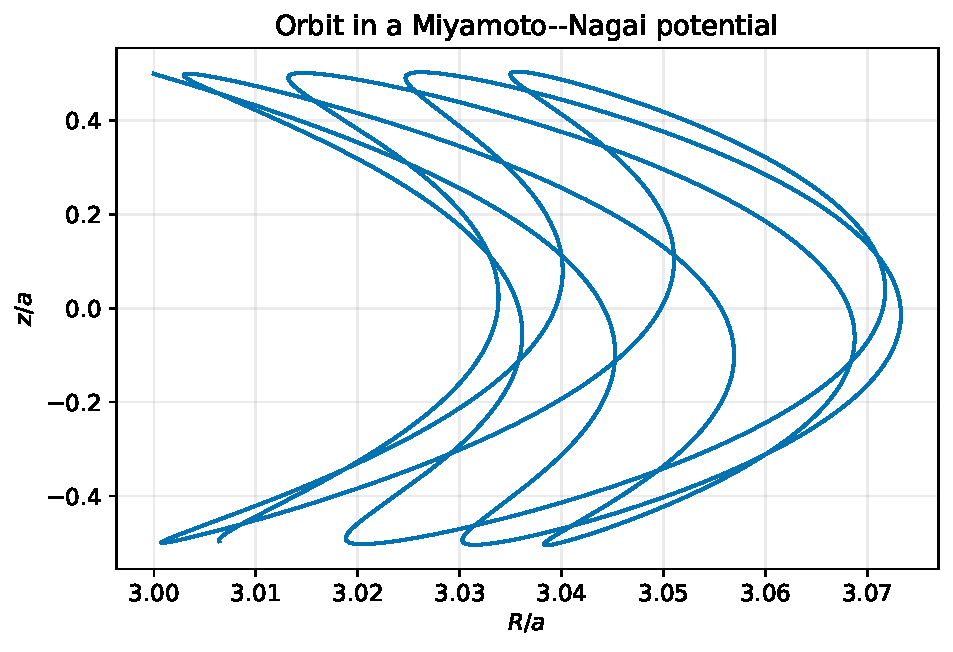
\includegraphics[width=0.64\linewidth]{appC_mn_orbit.pdf}
\caption{Miyamoto--Nagai ポテンシャル中の軌道の $R$--$z$ 平面への投影。積分時間は $100t_*$、時間刻みは $0.02t_*$ である。線の形だけで数値精度を判断せず、保存量と時間刻み依存性を合わせて確認する。}
\label{fig:appC-mn-orbit}
\end{figure}

\begin{cautionblock}{同じモデルでも数値重力場の誤差は別に検証する}
付録\ref{app:axisym-poisson}では同じモデルの密度から Poisson 方程式を解くが、その数値解は本節では使わない。
格子上のポテンシャルを軌道計算に使う場合には、空間離散化に加えて、補間や数値微分の誤差も含まれる。
また、モデルの厚さ $b/a$ を変える場合には、以前と同じ時間刻みで十分かを確かめ直す。
\end{cautionblock}

\section{非軸対称ポテンシャル}
\label{sec:appC-nonaxisymmetric}

\subsection{加速度と保存量の選択}

Ryden §7.3 の2次元の非軸対称対数ポテンシャル
\begin{equation}
 \Phi(x,y)=\frac12v_0^2\ln\left[1+\frac{x^2+y^2/q^2}{r_c^2}\right]
\label{eq:appC-nonaxisym-potential}
\end{equation}
を使う。これは Ryden 式(7.68) に対応する\cite{ryden2025}。
$v_0,r_c>0$、$0<q\le1$ とし、$q\ne1$ で非軸対称になる。
$D=r_c^2+x^2+y^2/q^2$ と置くと、加速度は
\begin{equation}
 g_x=-\frac{v_0^2x}{D},\qquad
 g_y=-\frac{v_0^2y}{q^2D}
\label{eq:appC-nonaxisym-acceleration}
\end{equation}
となる。
この場合は位置・速度・加速度を2成分の配列にするが、積分関数は同じでよい。

\begin{listingbox}{C.4　非軸対称対数ポテンシャルの加速度}
\begin{Verbatim}[fontsize=\small,xleftmargin=1mm]
def acc_nonaxisym(x, v0=1.0, rc=1.0, q=np.sqrt(3.0)/2.0):
    # 2次元の位置配列から、2成分の加速度を返す。
    X, Y = x
    den = rc**2 + X**2 + Y**2/q**2
    return -v0**2 * np.array([X, Y/q**2]) / den
\end{Verbatim}
\end{listingbox}


ポテンシャルは時間に依存しないため、
\begin{equation}
 E=\mathrm{const.}
\label{eq:appC-nonaxisym-energy}
\end{equation}
である。一方、式\eqref{eq:appC-nonaxisym-acceleration}から
\begin{equation}
 \frac{dL_z}{dt}=xg_y-yg_x
 =\frac{v_0^2xy}{D}\left(1-\frac1{q^2}\right)
\label{eq:appC-nonaxisym-torque}
\end{equation}
なので、$q\ne1$ では一般に
\begin{equation}
 L_z\ne\mathrm{const.}
\label{eq:appC-nonaxisym-lz}
\end{equation}
となる。
$L_z$ の変化をすべて数値誤差と解釈してはいけない。
$q=1$ とすればトルクが0になることは、加速度の実装を検証する一つの方法である。

\subsection{中心近傍の近似とその適用範囲}

中心近くで $\eta=(x^2+y^2/q^2)/r_c^2\ll1$ なら、
$\ln(1+\eta)=\eta+O(\eta^2)$ より
\begin{equation}
 \Phi(x,y)\simeq\frac12\frac{v_0^2}{r_c^2}x^2
 +\frac12\frac{v_0^2}{q^2r_c^2}y^2
\label{eq:appC-anisotropic-harmonic}
\end{equation}
となる。
この近似では $\ddot x=-\omega_x^2x$、$\ddot y=-\omega_y^2y$ であり、
\begin{equation}
 \omega_x=\frac{v_0}{r_c},\qquad \omega_y=\frac{v_0}{qr_c}
\end{equation}
という異方的調和振動子（anisotropic harmonic oscillator）になる。
$q<1$ では2方向の振動数が異なり、中心付近の運動を理解する手掛かりとなる。
ただし、以下の初期位置 $(2r_c,0)$ では $\eta=4$ であり、中心近傍の近似は成り立たない。
この近似を、有限振幅の数値軌道全体の基準解には使わない。

\subsection{同じエネルギーを持つ軌道の比較}

Ryden 図7.6 にならい、
\begin{equation}
 q=\frac{\sqrt3}{2},\qquad E=1.5v_0^2,\qquad
 \boldsymbol x_0=(2r_c,0)
\label{eq:appC-nonaxisym-params}
\end{equation}
を共通にする。
速さと速度方向を別々に設定し、
\begin{equation}
 v_{\rm init}=\sqrt{2[E-\Phi(2r_c,0)]},\qquad
 v_y=fv_{\rm init},\qquad
 v_x=+\sqrt{v_{\rm init}^2-v_y^2}
\label{eq:appC-nonaxisym-initial}
\end{equation}
とする。
$E>\Phi(2r_c,0)$、$0\le f\le1$ とすれば、平方根の中は非負である。
ここでは $f=0.5$ と $0.9$ を選び、初期位置とエネルギーを同じにしたまま、速度方向だけを変える。
$\Delta t=0.02r_c/v_0$、積分時間 $300r_c/v_0$ とし、Notebook C の既定値は $r_c=v_0=1$ である。

\begin{notebookblock}{C｜同じエネルギーを持つ2本の軌道}
\texttt{v0\_na}、\texttt{rc\_na}、\texttt{q\_na} をモデルのパラメータとし、\texttt{E\_target=1.5*v0\_na**2} とする。
まずエネルギーから速さを決め、速度方向を変えた2組の初期条件を作る。
\par\smallskip\noindent\begin{minipage}{\linewidth}
{\sffamily\small\color{graytext}対応セル（同じ比エネルギーからの初速度の設定）}
\begin{Verbatim}[fontsize=\footnotesize,xleftmargin=2mm,frame=single,framesep=1.8mm,framerule=0.35pt,rulecolor=\color{listingframe},fillcolor=\color{listingbg}]
# 初期位置と比エネルギーを共通にして速さを決める。
x_start = np.array([2.0 * rc_na, 0.0])
phi_start = phi_nonaxisym(x_start, v0_na, rc_na, q_na)
if E_target <= phi_start:
    raise ValueError("速度方向を比較するにはE_target > phi_startが必要です。")
speed = np.sqrt(2.0 * (E_target - phi_start))

# このモデルと初期位置でbox・loop軌道になる速度方向を選ぶ。
f_box = 0.50
vy_box = f_box * speed
vx_box = np.sqrt(speed**2 - vy_box**2)
v_box0 = np.array([vx_box, vy_box])
f_loop = 0.90
vy_loop = f_loop * speed
vx_loop = np.sqrt(speed**2 - vy_loop**2)
v_loop0 = np.array([vx_loop, vy_loop])
\end{Verbatim}
\end{minipage}

2本の軌道には、同じ加速度・時間刻み・終端時刻を使う。
\par\smallskip\noindent\begin{minipage}{\linewidth}
{\sffamily\small\color{graytext}対応セル（時間積分と診断量）}
\begin{Verbatim}[fontsize=\footnotesize,xleftmargin=2mm,frame=single,framesep=1.8mm,framerule=0.35pt,rulecolor=\color{listingframe},fillcolor=\color{listingbg}]
# 時間の単位をrc/v0に揃え、同じ刻みと終端時刻を使う。
dt_na = 0.02 * rc_na / v0_na
t_end_na = 300.0 * rc_na / v0_na
nstep_na = int(round(t_end_na / dt_na))
t_na = np.arange(nstep_na + 1) * dt_na
acc_na = lambda x: acc_nonaxisym(x, v0_na, rc_na, q_na)
x_box, v_box = integrate_leapfrog(acc_na, x_start, v_box0, dt_na, nstep_na)
x_loop, v_loop = integrate_leapfrog(acc_na, x_start, v_loop0, dt_na, nstep_na)

# Eの変化は保存誤差として、Lzの変化は物理的な変化として調べる。
E_box = energy_nonaxisym(x_box, v_box, v0_na, rc_na, q_na)
E_loop = energy_nonaxisym(x_loop, v_loop, v0_na, rc_na, q_na)
L_box = angular_momentum_z(x_box, v_box)
L_loop = angular_momentum_z(x_loop, v_loop)
\end{Verbatim}
\end{minipage}

\end{notebookblock}

図\ref{fig:appC-box}と図\ref{fig:appC-loop}に軌道を示す。
今回の計算時間では、$f=0.5$ の軌道は中心近傍まで達し、回り込む向きが変わる box 軌道である。
$f=0.9$ の軌道は、中心の周囲を一定の向きに回る loop 軌道である。
この分類は今回のモデルと初期条件についての結果であり、$f$ の値だけから任意の軌道を分類できるわけではない。

運動エネルギーが非負であるため、厳密な軌道が存在できる領域は $\Phi(x,y)\le E$ である。
その境界 $\Phi=E$ は
\begin{equation}
 x^2+\frac{y^2}{q^2}=r_c^2\left[\exp\left(\frac{2E}{v_0^2}\right)-1\right]
\label{eq:appC-zero-velocity}
\end{equation}
という楕円になり、図の破線に対応する。
これは許される領域を示すもので、軌道が内部のすべての点を通るという意味ではない。

\begin{figure}[!htbp]
\centering
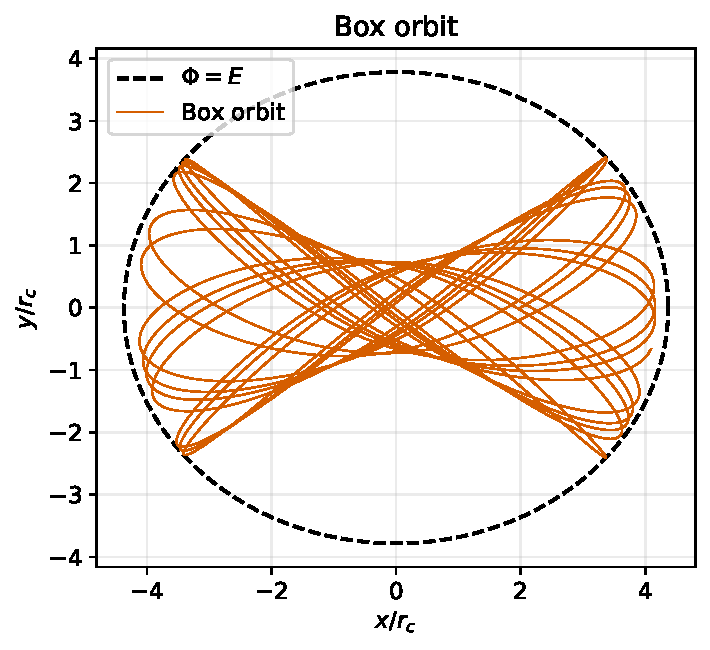
\includegraphics[width=0.51\linewidth]{appC_box_orbit.pdf}
\caption{$f=0.5$ の初速度で得た box 軌道。破線は式\eqref{eq:appC-zero-velocity}のゼロ速度境界 $\Phi=E$ である。積分時間は $300r_c/v_0$。}
\label{fig:appC-box}
\end{figure}

\begin{figure}[!htbp]
\centering
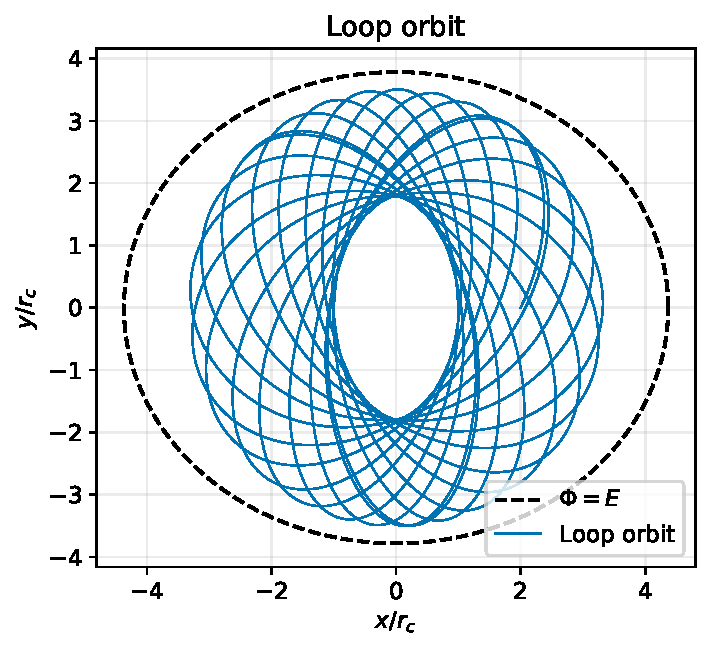
\includegraphics[width=0.51\linewidth]{appC_loop_orbit.pdf}
\caption{$f=0.9$ の初速度で得た loop 軌道。図\ref{fig:appC-box}と初期位置・比エネルギー・積分時間は同じであり、速度方向だけが異なる。}
\label{fig:appC-loop}
\end{figure}

\subsection{保存誤差と物理的な変化の区別}

両軌道の初期エネルギーは
\begin{equation}
 E_{\rm box}(0)=\appCBoxEnergy,\qquad
 E_{\rm loop}(0)=\appCLoopEnergy
\end{equation}
となり、設定どおり一致している。
$0\le t\le300r_c/v_0$ の全出力時刻で測ったエネルギーの最大絶対相対変化と角運動量の範囲を、表\ref{tab:appC-nonaxisym-diagnostics}に示す。
この場合、$E$ の変化は保存誤差として調べるが、$L_z$ の変化には式\eqref{eq:appC-nonaxisym-torque}のトルクによる物理的な変化が含まれる。

\begin{table}[!htbp]
\centering
\caption{非軸対称系の軌道の診断。$\epsilon_E$ は式\eqref{eq:appC-invariant-errors}で定義した保存誤差、$L_z$ の範囲は数値軌道に沿った変化であり、誤差の範囲ではない。}
\label{tab:appC-nonaxisym-diagnostics}
\begin{tabular}{ccc}
\toprule
軌道 & $\epsilon_E$ & $L_z/(r_cv_0)$ の範囲 \\
\midrule
box & $\appCBoxMaxEnergy$ & $[\appCBoxLzMin,\,\appCBoxLzMax]$ \\
loop & $\appCLoopMaxEnergy$ & $[\appCLoopLzMin,\,\appCLoopLzMax]$ \\
\bottomrule
\end{tabular}
\end{table}

図\ref{fig:appC-nonaxisym-lz}では、box 軌道の $L_z$ は正負を横切り、loop 軌道では符号が保たれる。
ただし、loop 軌道でも $L_z$ の大きさは一定ではない。
回り込む向きが変わらないことと、角運動量が保存することは別である。
数値的な変化と物理的な変化を区別するには、同じ初期条件・終端時刻で時間刻みを小さくし、エネルギー誤差が減っても $L_z(t)$ の変化が残るかを確かめる。

\begin{figure}[!htbp]
\centering
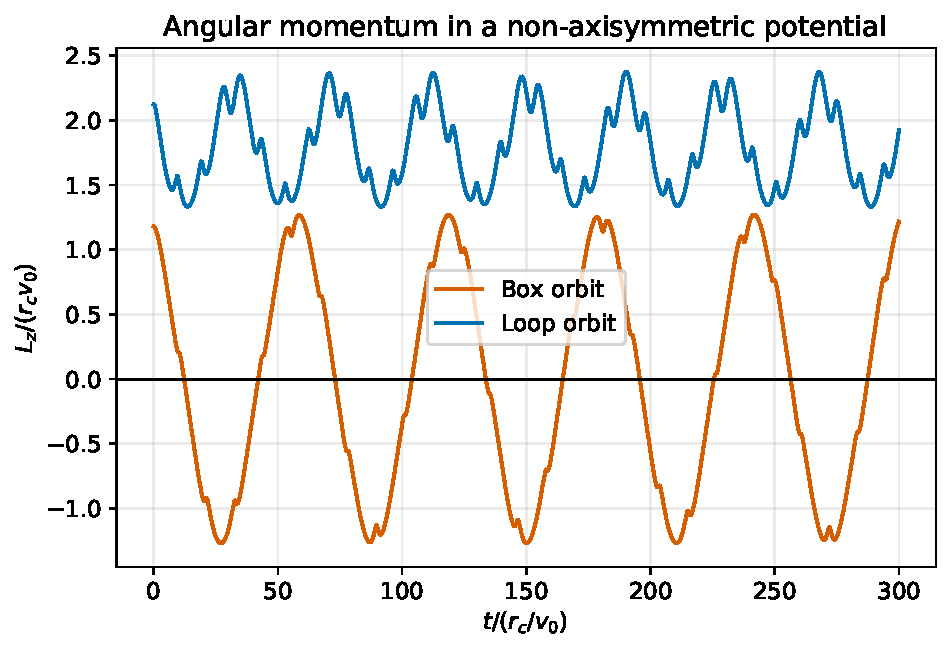
\includegraphics[width=0.64\linewidth]{appC_nonaxisym_Lz.pdf}
\caption{非軸対称対数ポテンシャル中の角運動量の時間変化。box 軌道では符号が変わり、loop 軌道では符号が保たれるが、どちらも一定ではない。}
\label{fig:appC-nonaxisym-lz}
\end{figure}

\begin{cautionblock}{有限時間の出力から判断できる範囲}
計算から直接得られる最小半径は、有限時間内の離散的な出力点で測った値である。
出力点の間でさらに小さい半径に達する可能性があり、積分時間を延ばせば新しい最小値が見つかる可能性もある。
積分時間と時間刻みを別々に変えて結果を比較する必要があるが、それだけで無限時間に中心へ任意に近づくことを証明したわけではない。
\end{cautionblock}


\chapter{連立一次方程式の解法}
\label{app:linear-systems}

第2章では \texttt{numpy.linalg.solve}、付録\ref{app:axisym-poisson}では \texttt{scipy.sparse.linalg.spsolve} を使い、
Poisson 方程式を離散化して得た連立一次方程式を解いた。
本付録は、その求解の仕組みを確認するための背景資料である。
同じ小さな連立一次方程式を使い、Gauss の消去法、LU 分解、疎行列の消去、Jacobi 法を順に説明する。
行列の構造と解法の種類を区別し、計算結果を残差でどう確認するかを学ぶ。
数値計算法は幸谷第7・8章\cite{kouya2021}を参考にする。

本編と同様に、一般的なソルバーの自作は求めない。
以下では $m$ 個の未知数に対する正方行列の問題 $A\boldsymbol u=\boldsymbol b$ を扱い、解は一意に定まるとする。
式と実装の対応は短い Listing で示す。付録D専用の Notebook は設けず、Notebook 2末尾の補足「付録D：連立一次方程式の解法」も参照できる。

\section{Gauss の消去法：小さな例}
\label{sec:appD-elimination}

第2章の三重対角行列と同じ構造を持つ、説明用の例を考える。
ここでは計算手順を追うため、右辺を $\boldsymbol b=(1,0,1)^{\mathsf T}$ と選ぶ。
この右辺は Plummer 球の密度や境界値から求めたものではない。連立一次方程式は
\begin{equation}
 \underbrace{\begin{pmatrix}2&-1&0\\-1&2&-1\\0&-1&2\end{pmatrix}}_{A}
 \begin{pmatrix}u_1\\u_2\\u_3\end{pmatrix}
 =\begin{pmatrix}1\\0\\1\end{pmatrix}
\label{eq:appD-example}
\end{equation}
である。これは、$2u_1-u_2=1$、$-u_1+2u_2-u_3=0$、$-u_2+2u_3=1$ の3式をまとめたものである。

一つの式の定数倍を別の式に加える操作は、同じ定数倍を引けば元に戻せるため、解を変えない。
この操作で未知数を順番に消す方法を\textbf{Gauss の消去法（Gaussian elimination）}と呼ぶ。
係数と右辺を縦線で区切って並べ、$R_i$ を第 $i$ 行と書くと、まず
\begin{equation}
 \left[\begin{array}{ccc|c}2&-1&0&1\\-1&2&-1&0\\0&-1&2&1\end{array}\right]
 \xrightarrow{\ R_2\leftarrow R_2+\frac12R_1\ }
 \left[\begin{array}{ccc|c}2&-1&0&1\\0&\frac32&-1&\frac12\\0&-1&2&1\end{array}\right]
\label{eq:appD-first-elimination}
\end{equation}
として、第2行の $u_1$ を消す。次に、\textbf{更新後の第2行}を使って
\begin{equation}
 R_3\leftarrow R_3+\frac23R_2
 \quad\Longrightarrow\quad
 \left[\begin{array}{ccc|c}2&-1&0&1\\0&\frac32&-1&\frac12\\0&0&\frac43&\frac43\end{array}\right]
\label{eq:appD-second-elimination}
\end{equation}
とすると、第3行の $u_2$ も消える。
このように対角成分より下を0にする操作が\textbf{前進消去（forward elimination）}である。
係数だけを変えると別の連立方程式になるため、右辺にも同じ行操作を行う。

得られた上三角の連立方程式は、下の行から順に解ける。
\begin{equation}
 u_3=\frac34\cdot\frac43=1,\qquad
 u_2=\frac23\left(\frac12+u_3\right)=1,\qquad
 u_1=\frac{1+u_2}{2}=1.
\label{eq:appD-back-substitution}
\end{equation}
この操作を\textbf{後退代入（back substitution）}と呼ぶ。
求めた解 $\boldsymbol u=(1,1,1)^{\mathsf T}$ を式\eqref{eq:appD-example}へ代入すると、元の3式を満たす。
\textbf{前進消去で解きやすい形に変え、後退代入で解を求める}のが基本である。

第2章と同じライブラリでこの例を解き、元の方程式に代入して確認するコードを Listing D.1に示す。
この例では厳密解が分かるので、残差だけでなく解そのものの誤差も計算できる。

\begin{listingbox}[left=6mm]{D.1　小さな連立一次方程式の求解と検証}
\begin{Verbatim}[fontsize=\small]
import numpy as np

A = np.array([[2.0, -1.0, 0.0], [-1.0, 2.0, -1.0], [0.0, -1.0, 2.0]])
b = np.array([1.0, 0.0, 1.0])
u_num = np.linalg.solve(A, b)

# 元の方程式の残差と、既知の厳密解からの誤差を別々に調べる
residual_max = np.max(np.abs(A @ u_num - b))
solution_error = np.max(np.abs(u_num - np.ones(3)))
\end{Verbatim}
\end{listingbox}

有限精度の計算では、解が見かけ上 $(1,1,1)$ と表示されても、残差が厳密に0になるとは限らない。
残差と解の誤差の違いは、\ref{sec:appD-iterative}節でも確認する。

\section{LU 分解：消去手順の行列表現}
\label{sec:appD-lu}

前節の行列 $A$ は、次の二つの三角行列の積に分解できる。
\begin{equation}
 \boxed{A=LU},\qquad
 L=\begin{pmatrix}1&0&0\\-\frac12&1&0\\0&-\frac23&1\end{pmatrix},\qquad
 U=\begin{pmatrix}2&-1&0\\0&\frac32&-1\\0&0&\frac43\end{pmatrix}.
\label{eq:appD-lu}
\end{equation}
$L$ は対角成分より上が0の下三角行列、$U$ は対角成分より下が0の上三角行列である。
ここでは $L$ の対角成分をすべて1に取っている。
この分解を\textbf{LU 分解（LU decomposition）}と呼ぶ。
$U$ は前進消去の結果で、$L$ には消去に使った倍率が記録されている。
例えば第2行の消去は $R_2\leftarrow R_2-\ell_{21}R_1$ と書け、
$\ell_{21}=-1/2$ である。これが $L$ の第2行・第1列の値になる。
同様に、更新後の第2行を使う倍率 $\ell_{32}=-2/3$ が $L$ に入る。

$A\boldsymbol u=\boldsymbol b$ に $A=LU$ を代入し、$\boldsymbol y=U\boldsymbol u$ とおけば、
\begin{equation}
 \underbrace{L\boldsymbol y=\boldsymbol b}_{\text{上の行から解く}}
 \qquad\longrightarrow\qquad
 \underbrace{U\boldsymbol u=\boldsymbol y}_{\text{下の行から解く}}
\label{eq:appD-triangular-solves}
\end{equation}
の2段階になる。下三角系を上から解く操作が\textbf{前進代入（forward substitution）}である。
本例では
\begin{equation}
 y_1=1,\qquad
 y_2=0+\frac12y_1=\frac12,\qquad
 y_3=1+\frac23y_2=\frac43
\label{eq:appD-forward-substitution}
\end{equation}
となり、$\boldsymbol y$ は式\eqref{eq:appD-second-elimination}の変形後の右辺に一致する。
あとは前節と同じ後退代入で $\boldsymbol u$ を求める。
\textbf{前進消去は行列を変形する操作、前進代入は下三角系を解く操作}である。

同じ $A$ に対して右辺 $\boldsymbol b$ だけが変わる場合、一度求めた $L,U$ を再利用できる。
各右辺について前進代入と後退代入だけを行えばよいことが、LU 分解の利点である\cite{kouya2021}。
第2章の Poisson 方程式でも、格子と差分式を固定して密度や境界値だけを変えるなら、係数行列は変わらず右辺だけが変わる。
ただし、格子を変える収束試験では行列も変わるので、同じ分解をそのまま使うことはできない。

\subsection{行を入れ替える場合}
一般の行列では、解が一意に定まっていても、消去の途中で割る成分が0になることがある。
0でなくても、他の成分に比べて小さい値で割ると、丸め誤差が増幅される場合がある。
この割る成分を\textbf{枢軸（pivot、ピボット）}という。
\textbf{部分枢軸選択（partial pivoting）}では、処理する列の未処理部分から絶対値が最大の成分を選び、
その行を現在の行と入れ替える。右辺も同じ順に入れ替える。
行の入れ替えを表す行列を $P$ と書けば、本書の記法では
\begin{equation}
 PA=LU,\qquad L\boldsymbol y=P\boldsymbol b,\qquad U\boldsymbol u=\boldsymbol y
\label{eq:appD-pivot-lu}
\end{equation}
となる。行を入れ替えても未知数の順番は変わらない。
本例では行交換は不要である\cite{kouya2021}。

\subsection{なぜ逆行列を作らずに \texttt{solve} を使うのか}
数学的には $\boldsymbol u=A^{-1}\boldsymbol b$ と書けるが、解だけが必要なら逆行列全体を作る必要はない。
逆行列を求めてから右辺を掛ける方法は、LU 分解と代入で解く方法より計算量が増える\cite{kouya2021}。
第2章と Listing D.1の \texttt{np.linalg.solve(A, b)} も、逆行列を明示的に作るのではなく、LU 分解を用いて解を求める。

消去法や LU 分解のように、所定の消去・代入で解を求める方法を\textbf{直接法（direct method）}と呼ぶ。
ただし、計算機では丸め誤差があるため、「直接法」は「誤差がない方法」という意味ではない。

\section{疎行列の消去と代入}
\label{sec:appD-sparse}

付録\ref{app:axisym-poisson}で定義した「疎行列」は、0の要素が多いという\textbf{行列の構造}を表し、解法の名前ではない。
疎行列にも前節の LU 分解を使える。
違いは、0の要素まで一律に保存・計算するのではなく、\textbf{必要な非零要素を扱いながら消去と代入を進める}ことである。
まず前節と同じ三重対角系で、その計算を具体的に見る。

\subsection{三重対角行列と Thomas 法}

式\eqref{eq:appD-example}の行列では、第1列で消す必要があるのは第2行の $-1$ だけである。
第3行の第1成分は初めから0なので、第1行を使って第3行を更新する必要はない。
第2列でも、更新するのは第3行だけである。

この行列を、対角が2、隣接する副対角が $-1$ の $m$ 次三重対角行列へ拡張する。
未知数は $u_1,\ldots,u_m$ で、両端の式には範囲外の未知数を含めない。
消去後の第 $i-1$ 行が
\begin{equation*}
 d_{i-1}u_{i-1}-u_i=y_{i-1}
\end{equation*}
になったとする。次の行 $-u_{i-1}+2u_i-u_{i+1}=b_i$ に、その $1/d_{i-1}$ 倍を加えると、
\begin{equation}
 \left(2-\frac{1}{d_{i-1}}\right)u_i-u_{i+1}
 =b_i+\frac{y_{i-1}}{d_{i-1}}
\label{eq:appD-sparse-row}
\end{equation}
となり、$u_{i-1}$ が消える。つまり、更新が必要なのは対角成分と右辺だけである。
\begin{equation}
 d_1=2,\quad y_1=b_1,\qquad
 d_i=2-\frac{1}{d_{i-1}},\quad
 y_i=b_i+\frac{y_{i-1}}{d_{i-1}}\quad(i=2,\ldots,m).
\label{eq:appD-tridiagonal-forward}
\end{equation}
最後の行には $u_{m+1}$ がないので $d_mu_m=y_m$ である。下の行から
\begin{equation}
 u_m=\frac{y_m}{d_m},\qquad
 u_i=\frac{y_i+u_{i+1}}{d_i}\quad(i=m-1,\ldots,1)
\label{eq:appD-tridiagonal-back}
\end{equation}
と代入すれば解が得られる。

前節の $\boldsymbol b=(1,0,1)^{\mathsf T}$ では、計算する数は次のとおりである。
\begin{table}[H]
\centering
\caption{3未知数の例で、前進消去により更新される対角成分と右辺。}
\label{tab:appD-thomas}
\renewcommand{\arraystretch}{1.25}
\begin{tabular}{ccl}
\toprule
行 $i$ & 消去後の対角 $d_i$ & 消去後の右辺 $y_i$ \\
\midrule
1 & $2$ & $1$ \\
2 & $2-1/2=3/2$ & $0+1/2=1/2$ \\
3 & $2-1/(3/2)=4/3$ & $1+(1/2)/(3/2)=4/3$ \\
\bottomrule
\end{tabular}
\end{table}
これは式\eqref{eq:appD-second-elimination}と同じ結果である。
式\eqref{eq:appD-tridiagonal-back}から、再び $u_3=u_2=u_1=1$ を得る。
新しい解法へ置き換えたのではなく、\textbf{同じ消去法から0に対する不要な操作を省いている}。

三重対角行列の非零要素は $3m-2$ 個である。この例では各行を1回ずつ消去・代入するため、演算回数と記憶量は $m$ に比例する。
このように三重対角系の構造を利用して前進消去と後退代入を行う手順は、\textbf{Thomas 法（Thomas algorithm）}と呼ばれる。

この例では、式\eqref{eq:appD-tridiagonal-forward}から
\begin{equation}
 d_i=\frac{i+1}{i}>0\qquad(i=1,\ldots,m)
\label{eq:appD-positive-pivots}
\end{equation}
となる。実際、$d_{i-1}=i/(i-1)$ を漸化式に代入すれば $d_i=(i+1)/i$ を得る。
したがって、この係数行列では0で割ることはない。
一般の三重対角行列では、係数に応じて漸化式が変わり、消去中に割る成分が0または非常に小さくなる場合もある。
三重対角という構造だけで、行交換なしの消去が常に使えるわけではない。

\subsection{一般の疎行列とフィルイン}

三重対角の例では、消去後も隣接した成分だけを扱えた。
一方、付録\ref{app:axisym-poisson}のような2次元の問題では、消去によって最初は0だった位置にも非零の値が生じる。
ここでは、両方向の格子幅を $h$ とする直交格子で、2行2列の内部点を行ごとに番号付けした4未知数の例を使う。
2次元 Poisson 方程式の5点差分式に $-h^2$ を掛け、既知の境界値を右辺へ移すと、係数行列は次の形になる。
\begin{equation}
 B=\begin{pmatrix}
 4&-1&-1&0\\
 -1&4&0&-1\\
 -1&0&4&-1\\
 0&-1&-1&4
 \end{pmatrix}
\label{eq:appD-sparse2d-example}
\end{equation}
付録\ref{app:axisym-poisson}の軸対称系とは係数が異なるが、隣接点が結び付く構造は共通である。

第1列を消すために $R_2\leftarrow R_2+\frac14R_1$ とすると、第2行は
\begin{equation}
 (-1,4,0,-1)+\frac14(4,-1,-1,0)
 =\left(0,\frac{15}{4},-\frac14,-1\right)
\label{eq:appD-fill-example}
\end{equation}
へ変わる。\textbf{第2行・第3列の0が $-1/4$ に変わった。}
このように消去で新たに生じる非零要素を\textbf{フィルイン（fill-in）}と呼ぶ。
疎行列の直接法でも、この成分を無視してよいわけではなく、保存して以後の計算に使う。


図\ref{fig:appD-sparse-fill-in}は、二つの例について前進消去の前後の非零要素の位置を比較したものである。
三重対角行列では新たな非零位置は生じないが、行列 $B$ では上三角行列 $U_B$ の第2行・第3列にフィルインが残る。
フィルインとは、元は0だった位置に値が生じることを指す。下三角部分を消しているため、図の前後で非零要素の総数が増えるとは限らない。

\begin{figure}[H]
\centering
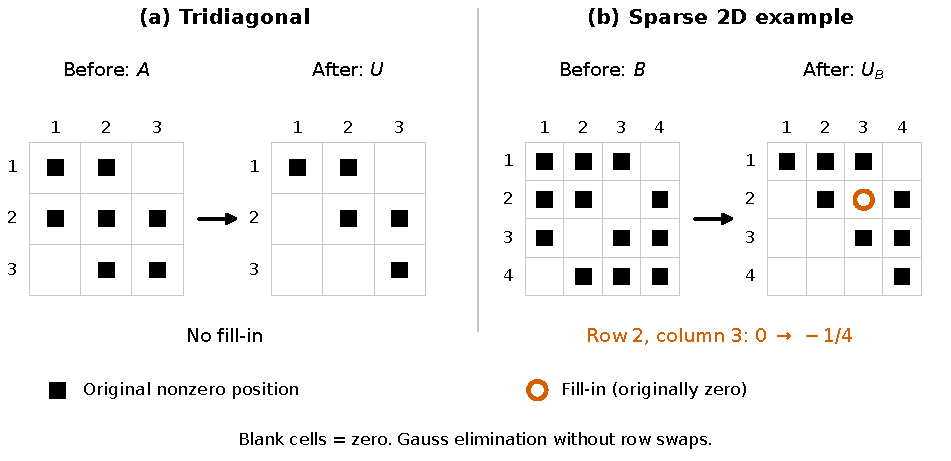
\includegraphics[width=\linewidth]{appD_sparse_elimination_fillin.pdf}
\caption{疎行列の前進消去と新たに生じる非零要素（フィルイン）。行交換を行わず、(a) 式\eqref{eq:appD-example}の $A$ と消去後の $U$、
(b) 式\eqref{eq:appD-sparse2d-example}の $B$ と消去後の $U_B$ を比較している。
黒い四角は元の行列でも非零だった位置、朱色の白抜き丸は元は0だった位置に生じた非零要素を表し、空白は0である。
(b) の第2行・第3列の値は、式\eqref{eq:appD-fill-example}で求めた $-1/4$ である。
記号は非零の位置だけを表し、係数の大きさや符号は表していない。}
\label{fig:appD-sparse-fill-in}
\end{figure}

図\ref{fig:appD-sparse-fill-in}に示したのは $U$ の非零位置だけであり、実際の LU 分解では $L$ も保存する。
必要な記憶量は、元の行列の非零要素数だけでは決まらない。
疎行列の LU 分解では、非零要素の位置を管理しながら消去を行い、得られた三角行列に前進代入と後退代入を行う。
非零要素の増加を抑えるために未知数の順を並べ替え、数値的な安定性のために行を入れ替えることもある。
\textbf{基本はあくまで LU 分解と代入であり、疎な構造に合わせて計算と保存の方法を工夫している。}

\subsection{第2章の \texttt{solve} と付録Bの \texttt{spsolve} の違い}
第2章の \texttt{numpy.linalg.solve} は、三重対角行列を入力しても密行列として扱う。
第2章では差分式と行列の対応を見やすくするためにこの方法を使ったが、\eqref{eq:appD-tridiagonal-forward}--\eqref{eq:appD-tridiagonal-back}の手順を自動的に使っているわけではない。
付録\ref{app:axisym-poisson}の \texttt{spsolve} は、ここで述べた疎行列の直接法を使う。
幸谷第8章でも、\texttt{spsolve} による求解と、疎な LU 分解を保存して再利用する方法が説明されている\cite{kouya2021}。
\texttt{spsolve} は、次節で扱う反復法ではない。
また、疎行列を入力しただけで演算回数が未知数の数に比例するとは限らず、フィルインや並べ替えの影響も受ける。

\clearpage
\section{反復法：Jacobi 法}
\label{sec:appD-iterative}

直接法では行列を変形したが、\textbf{反復法（iterative method）}では近似解を繰り返し更新する。
ここでは幸谷第8章の\textbf{Jacobi 法（Jacobi method）}を、同じ3未知数の例へ適用する\cite{kouya2021}。

\subsection{反復式への書き換え}

式\eqref{eq:appD-example}の各行を、それぞれ $u_1,u_2,u_3$ について解くと、
\begin{equation}
 u_1=\frac{1+u_2}{2},\qquad
 u_2=\frac{u_1+u_3}{2},\qquad
 u_3=\frac{1+u_2}{2}
\label{eq:appD-jacobi-rearrange}
\end{equation}
である。このままでは右辺にも未知数がある。
そこで右辺には\textbf{現在の近似値}を入れ、左辺を\textbf{次の近似値}として計算する。
$k$ 回目の近似解を $\boldsymbol u^{(k)}$ とすると、
\begin{equation}
 \boxed{
 \begin{aligned}
 u_1^{(k+1)}&=\frac{1+u_2^{(k)}}{2},\\
 u_2^{(k+1)}&=\frac{u_1^{(k)}+u_3^{(k)}}{2},\\
 u_3^{(k+1)}&=\frac{1+u_2^{(k)}}{2}
 \end{aligned}}
\label{eq:appD-jacobi-update}
\end{equation}
となる。上付きの $(k)$ は反復回数であり、物理的な時刻ではない。
Jacobi 法では、\textbf{右辺のすべての成分に、更新前の同じ $k$ 回目の値を使う}。
Listing D.2では、更新前の配列 \texttt{u\_old} と更新後の配列 \texttt{u\_new} を分けて、最初の1回の更新を示す。
NumPy は Listing D.1と同様に \texttt{np} という名前で読み込んでおく。

\begin{listingbox}[left=6mm]{D.2　Jacobi 法の1回の更新}
\begin{Verbatim}[fontsize=\small]
u_old = np.zeros(3)

# すべての成分を、更新前の同じ配列から計算する
u_new = np.empty_like(u_old)
u_new[0] = (1.0 + u_old[1]) / 2.0
u_new[1] = (u_old[0] + u_old[2]) / 2.0
u_new[2] = (1.0 + u_old[1]) / 2.0
u_old = u_new
\end{Verbatim}
\end{listingbox}

1行目の初期化は最初に1回だけ行う。以後は4--8行目を繰り返す。
各反復で新しい配列を作り、三つの値をすべて計算してから次の反復へ渡す。
計算途中で \texttt{u\_old} の成分を書き換えて右辺に使うと、式\eqref{eq:appD-jacobi-update}とは別の更新になる。

\subsection{初期値からの反復計算}

初期値を $\boldsymbol u^{(0)}=(0,0,0)^{\mathsf T}$ とする。1回目は
\begin{equation*}
 \boldsymbol u^{(1)}
 =\left(\frac{1+0}{2},\frac{0+0}{2},\frac{1+0}{2}\right)^{\mathsf T}
 =\left(\frac12,0,\frac12\right)^{\mathsf T},
\end{equation*}
2回目は、この三つの値を使って
\begin{equation*}
 \boldsymbol u^{(2)}
 =\left(\frac{1+0}{2},\frac{1/2+1/2}{2},\frac{1+0}{2}\right)^{\mathsf T}
 =\left(\frac12,\frac12,\frac12\right)^{\mathsf T}
\end{equation*}
となる。1回目には端の二つだけが変わり、2回目にはその影響が中央へ伝わっている。

以後の計算結果を表\ref{tab:appD-jacobi}に示す。
残差は第2章と同じ $\boldsymbol r_{\rm res}^{(k)}=A\boldsymbol u^{(k)}-\boldsymbol b$ とし、その最大絶対成分も併記する。

\begin{table}[H]
\centering
\caption{Jacobi 法の近似解と最大残差。残差は、表示用に丸める前の近似解から計算した。}
\label{tab:appD-jacobi}
\renewcommand{\arraystretch}{1.12}
\begin{tabular}{rcccc}
\toprule
反復回数 $k$ & $u_1^{(k)}$ & $u_2^{(k)}$ & $u_3^{(k)}$ & $\max_i|r_{{\rm res},i}^{(k)}|$ \\
\midrule
0 & 0 & 0 & 0 & 1 \\
1 & 0.5 & 0 & 0.5 & 1 \\
2 & 0.5 & 0.5 & 0.5 & 0.5 \\
3 & 0.75 & 0.5 & 0.75 & 0.5 \\
4 & 0.75 & 0.75 & 0.75 & 0.25 \\
10 & 0.968750 & 0.968750 & 0.968750 & 0.031250 \\
20 & 0.999023 & 0.999023 & 0.999023 & 0.000977 \\
\bottomrule
\end{tabular}
\end{table}
直接法で得た $\boldsymbol u=(1,1,1)^{\mathsf T}$ に近づいている。
この初期値では、偶数回の更新後に三つの成分が等しくなる。
その共通の値を $c$ とすると、式\eqref{eq:appD-jacobi-update}を2回使った後の値は $(1+c)/2$ なので、厳密解1からのずれが半分になる。
したがって、
\begin{equation}
 \boldsymbol u^{(2\ell)}=(1-2^{-\ell})(1,1,1)^{\mathsf T}\qquad(\ell=0,1,\ldots)
\label{eq:appD-jacobi-even}
\end{equation}
であり、途中の奇数回の値も同じ厳密解へ近づく。
これはこの行列と初期値に対する結果であり、一般の行列についての収束保証ではない。

\subsection{収束判定と疎行列での計算}

実際の計算では、元の行列と右辺を用いて残差を調べる。
表\ref{tab:appD-jacobi}の例では、$k=20$ で最大残差は $2^{-10}\simeq9.77\times10^{-4}$ である。
例えば最大残差が $10^{-3}$ 未満になったら止めると決めれば、20回目に初めてこの条件を満たす。
丸めて表示した値ではなく、計算中の配列から判定する。

ただし、残差の絶対値は方程式の規格化に依存する。
$A$ と $\boldsymbol b$ を同じ非零の定数倍にしても解は変わらないが、残差はその定数倍になる。
許容値は、右辺の大きさや問題の単位に合わせて設定する必要がある。
また、最大反復数も決め、条件を満たさずにその回数へ達した場合は、収束したとは扱わない。

残差は解の誤差そのものでもない。
連立一次方程式の厳密解を $\boldsymbol u_\ast$、現在の誤差を $\boldsymbol e^{(k)}=\boldsymbol u^{(k)}-\boldsymbol u_\ast$ とすると、
\begin{equation}
 \boldsymbol r_{\rm res}^{(k)}
 =A\boldsymbol u^{(k)}-\boldsymbol b
 =A(\boldsymbol u^{(k)}-\boldsymbol u_\ast)
 =A\boldsymbol e^{(k)}
\label{eq:appD-residual-error}
\end{equation}
である。このため、残差と解の誤差は一般には同じ大きさではなく、その関係は行列にも依存する\cite{kouya2021}。
本例のように厳密解が分かる場合は、Listing D.1のように両方を確認できる。

一般の行列でも、各行を同じように書き直せば
\begin{equation}
 u_i^{(k+1)}
 =\frac{b_i-\displaystyle\sum_{j\ne i}a_{ij}u_j^{(k)}}{a_{ii}}
 \qquad(a_{ii}\ne0)
\label{eq:appD-jacobi-general}
\end{equation}
となる。$a_{ij}=0$ の項は和に寄与しないので、疎行列では非零要素だけを使える。
三重対角の例なら各点の更新に使うのは隣の二つの近似値だけで、$L,U$ を作る必要はない。
ただし、必要な反復回数は行列や許容値に依存し、大きな問題では収束が遅くなることもある。
\textbf{疎行列という構造は、直接法でも反復法でも利用できる。}

\begin{cautionblock}{反復の収束と格子収束は別の確認}
反復回数を増やすときは、格子を固定した同じ連立一次方程式を解いている。
反復が収束しても、その方程式を作った有限差分の離散化誤差は残る。
第2章や付録\ref{app:axisym-poisson}の格子収束試験では、格子を細かくして別の連立一次方程式を作り、元の Poisson 方程式の解への近づき方を調べる。
反復法を使う場合は、各格子で許容値をさらに小さくしても結果がほとんど変わらないことを確認し、求解が不十分なことによる誤差を格子収束に混ぜない。
\end{cautionblock}

Jacobi 法は反復法の最も基本的な例の一つである。
ほかにも、Gauss--Seidel 法や、対称正定値行列に対する
共役勾配法（conjugate gradient method）などがある。
また、付録\ref{app:axisym-poisson}の補足で紹介した多重格子法は、異なる格子幅の問題を組み合わせて誤差を効率よく減らす方法である。
本書では、これらの詳細には立ち入らない。

% Appendix E: 数学公式集
% 既存の本文で \appendix を宣言し、付録 A--D に続けて \input する。
% 必要なパッケージ: amsmath, amssymb, booktabs, longtable, titlesec, needspace
% Compact layout settings (scoped to this appendix only).
% Designed for the book's A4 layout and an optional A5 handout.
\begingroup
% 各数式の先頭を左揃えにするため、以下の数式には flalign* を使用する。
% & は左端のアンカーであり、等号の位置を揃える目的には使わない。
\titlespacing*{\chapter}{0pt}{0pt}{6pt}
\titlespacing*{\section}{0pt}{0.45em}{0.12em}
\titlespacing*{\subsection}{0pt}{0.32em}{0.08em}
\small
\linespread{1.0}\selectfont
\setlength{\parskip}{0pt}
\setlength{\abovedisplayskip}{3pt plus 1pt minus 1pt}
\setlength{\belowdisplayskip}{3pt plus 1pt minus 1pt}
\setlength{\abovedisplayshortskip}{2pt plus 1pt minus 1pt}
\setlength{\belowdisplayshortskip}{2pt plus 1pt minus 1pt}
\setlength{\jot}{1.5pt}
\setlength{\tabcolsep}{3.5pt}
\renewcommand{\arraystretch}{0.97}
\setlength{\LTpre}{3pt}
\setlength{\LTpost}{3pt}
\allowdisplaybreaks[2]
\chapter{数学公式集}\label{app:math-formulas}

この付録では、本文および付録の計算でよく使う数学公式をまとめる。
特に断らない限り、$\log x$ は自然対数、角度はラジアンで表す。
$u,v$ は微分可能な関数、$f$ は必要な階数まで微分可能な関数とする。
ベクトルの内積・外積にはそれぞれ $\cdot,\times$ を用いる。

\section{基本的な記号、指数・対数}\label{sec:app-math-basic}
\subsection{階乗と二項定理}
\begin{flalign*}
 & n!= n(n-1)\cdots 2\cdot 1, \qquad 0!=1 && \\
 & \binom{n}{k}= \frac{n!}{k!(n-k)!} \qquad (0\le k\le n) && \\
 & (a+b)^n= \sum_{k=0}^{n}\binom{n}{k}a^{n-k}b^k \qquad (n=0,1,2,\ldots) &&
\end{flalign*}

\subsection{指数と対数}
\begin{flalign*}
 & a^{x+y}=a^xa^y && \\
 & a^{-x}=\frac{1}{a^x} && \\
 & \log(xy)=\log x+\log y && \\
 & \log\frac{x}{y}=\log x-\log y && \\
 & \log(x^p)=p\log x && \\
 & \log_a x=\frac{\log x}{\log a} && \\
 & e^{\log x}=x\quad(x>0) && \\
 & \log(e^x)=x &&
\end{flalign*}
ここで、対数の引数は正、$a>0$ とし、対数の底として $a\ne1$ を仮定する。
また、$\log_{10} x=(\log x)/(\log 10)$ である。

\section{三角関数と双曲線関数}\label{sec:app-math-trig}
\subsection{三角関数の基本公式}
\begin{flalign*}
 & \sin^2x+\cos^2x=1 && \\
 & 1+\tan^2x=\frac{1}{\cos^2x} && \\
 & \sin(x\pm y)=\sin x\cos y\pm\cos x\sin y && \\
 & \cos(x\pm y)=\cos x\cos y\mp\sin x\sin y && \\
 & \tan(x\pm y)=\frac{\tan x\pm\tan y}{1\mp\tan x\tan y} &&
\end{flalign*}
\begin{flalign*}
 & \sin x+\sin y=2\sin\frac{x+y}{2}\cos\frac{x-y}{2} && \\
 & \sin x-\sin y=2\cos\frac{x+y}{2}\sin\frac{x-y}{2} && \\
 & \cos x+\cos y=2\cos\frac{x+y}{2}\cos\frac{x-y}{2} && \\
 & \cos x-\cos y=-2\sin\frac{x+y}{2}\sin\frac{x-y}{2} &&
\end{flalign*}
\begin{flalign*}
 & 2\sin x\sin y=\cos(x-y)-\cos(x+y) && \\
 & 2\cos x\cos y=\cos(x-y)+\cos(x+y) && \\
 & 2\sin x\cos y=\sin(x+y)+\sin(x-y) && \\
 & \sin 2x=2\sin x\cos x && \\
 & \cos 2x=\cos^2x-\sin^2x=1-2\sin^2x=2\cos^2x-1 && \\
 & \sin 3x=3\sin x-4\sin^3x && \\
 & \cos 3x=4\cos^3x-3\cos x &&
\end{flalign*}
角度の換算は $180^\circ=\pi\,\mathrm{rad}$ である。

\subsection{双曲線関数}
\begin{flalign*}
 & \sinh x=\frac{e^x-e^{-x}}{2} && \\
 & \cosh x=\frac{e^x+e^{-x}}{2} && \\
 & \tanh x=\frac{\sinh x}{\cosh x} && \\
 & \cosh^2x-\sinh^2x=1 && \\
 & \sinh(x\pm y)=\sinh x\cosh y\pm\cosh x\sinh y && \\
 & \cosh(x\pm y)=\cosh x\cosh y\pm\sinh x\sinh y && \\
 & \sinh 2x=2\sinh x\cosh x && \\
 & \cosh 2x=2\cosh^2x-1=1+2\sinh^2x &&
\end{flalign*}
さらに、逆双曲線関数は\(\operatorname{arsinh}x=\log(x+\sqrt{1+x^2})\)、\(\operatorname{arcosh}x=\log(x+\sqrt{x^2-1})\)（$x\ge1$）と表せる。

\section{微分の公式}\label{sec:app-math-diff}
\subsection{基本法則}
ダッシュは $x$ による微分を表す。
\begin{flalign*}
 & (au+bv)'=au'+bv' && \\
 & (uv)'=u'v+uv' && \\
 & \left(\frac{u}{v}\right)'=\frac{u'v-uv'}{v^2} && \\
 & (u^p)'=pu^{p-1}u' && \\
 & \frac{\mathrm d}{\mathrm dx}f(g(x))=f'(g(x))g'(x) &&
\end{flalign*}
最後の公式は合成関数の微分（連鎖律）である。

\subsection{初等関数の導関数}
\begin{center}\small
\begin{tabular}{@{}ll@{\qquad}ll@{}}
\toprule
$f(x)$ & $f'(x)$ & $f(x)$ & $f'(x)$\\
\midrule
$x^p$ & $px^{p-1}$ & $e^{ax}$ & $ae^{ax}$\\
$a^x$ & $a^x\log a$ & $\log|x|$ & $1/x$\\
$\sin x$ & $\cos x$ & $\cos x$ & $-\sin x$\\
$\tan x$ & $1/\cos^2 x$ & $\arctan x$ & $1/(1+x^2)$\\
$\arcsin x$ & $1/\sqrt{1-x^2}$ & $\arccos x$ & $-1/\sqrt{1-x^2}$\\
$\sinh x$ & $\cosh x$ & $\cosh x$ & $\sinh x$\\
$\tanh x$ & $1/\cosh^2 x$ & $\sqrt{1+x^2}$ & $x/\sqrt{1+x^2}$\\
\bottomrule
\end{tabular}
\end{center}
適用範囲では各関数の引数・分母・平方根の条件を満たすものとする。

\section{積分の公式}\label{sec:app-math-int}
\subsection{基本法則と不定積分}
\begin{flalign*}
 & \int (au+bv)\,\mathrm dx=a\int u\,\mathrm dx+b\int v\,\mathrm dx && \\
 & \int uv'\,\mathrm dx=uv-\int u'v\,\mathrm dx && \\
 & \int f(g(x))g'(x)\,\mathrm dx=\int f(t)\,\mathrm dt\quad(t=g(x)) &&
\end{flalign*}
\begin{flalign*}
 & \int x^p\,\mathrm dx=\frac{x^{p+1}}{p+1}+C\quad(p\ne-1) && \\
 & \int\frac{\mathrm dx}{x}=\log|x|+C && \\
 & \int e^{ax}\,\mathrm dx=\frac{e^{ax}}{a}+C\quad(a\ne0) && \\
 & \int\sin x\,\mathrm dx=-\cos x+C && \\
 & \int\cos x\,\mathrm dx=\sin x+C && \\
 & \int x\sin x\,\mathrm dx=\sin x-x\cos x+C && \\
 & \int x\cos x\,\mathrm dx=\cos x+x\sin x+C && \\
 & \int\frac{\mathrm dx}{x^2+a^2}=\frac{1}{a}\arctan\frac{x}{a}+C\quad(a>0) && \\
 & \int\frac{\mathrm dx}{\sqrt{a^2-x^2}}=\arcsin\frac{x}{a}+C\quad(a>0) && \\
 & \int\frac{\mathrm dx}{\sqrt{x^2+a^2}}=\log\left|x+\sqrt{x^2+a^2}\right|+C &&
\end{flalign*}
指数関数と三角関数の積については、$a^2+b^2>0$ として
\begin{flalign*}
 & \int e^{ax}\sin bx\,\mathrm dx=\frac{e^{ax}}{a^2+b^2}(a\sin bx-b\cos bx)+C && \\
 & \int e^{ax}\cos bx\,\mathrm dx=\frac{e^{ax}}{a^2+b^2}(a\cos bx+b\sin bx)+C &&
\end{flalign*}

\subsection{代表的な定積分とガウス積分}
$a>0$ のとき、
\begin{flalign*}
 & \int_0^\infty e^{-ax}\,\mathrm dx=\frac{1}{a} && \\
 & \int_0^\infty\frac{a\,\mathrm dx}{x^2+a^2}=\frac{\pi}{2} && \\
 & \int_0^\infty e^{-ax^2}\,\mathrm dx=\frac12\sqrt{\frac{\pi}{a}} && \\
 & \int_{-\infty}^{\infty}e^{-ax^2}\,\mathrm dx=\sqrt{\frac{\pi}{a}} && \\
 & \int_0^\infty x^2e^{-ax^2}\,\mathrm dx=\frac14\sqrt{\frac{\pi}{a^3}} && \\
 & \int_0^\infty e^{-ax^2}\cos(bx)\,\mathrm dx=\frac12\sqrt{\frac{\pi}{a}}e^{-b^2/(4a)} &&
\end{flalign*}

\section{テイラー展開}\label{sec:app-math-taylor}
\subsection{一般式と近似誤差}
$h=x-a$ とすると、十分滑らかな $f$ に対して
\begin{flalign*}
 & f(a+h)=f(a)+hf'(a)+\frac{h^2}{2!}f''(a)+\cdots+\frac{h^n}{n!}f^{(n)}(a)+R_{n+1} && \\
 & R_{n+1}=\frac{h^{n+1}}{(n+1)!}f^{(n+1)}(\xi), \qquad \xi\text{ は }a\text{ と }a+h\text{ の間} &&
\end{flalign*}
$f^{(n+1)}$ が近傍で有界であれば $R_{n+1}=O(h^{n+1})$ である。

\subsection{主なマクローリン展開}
\begin{flalign*}
 & e^x=1+x+\frac{x^2}{2!}+\frac{x^3}{3!}+\cdots && \\
 & \sin x=x-\frac{x^3}{3!}+\frac{x^5}{5!}-\cdots && \\
 & \cos x=1-\frac{x^2}{2!}+\frac{x^4}{4!}-\cdots && \\
 & \sinh x=x+\frac{x^3}{3!}+\frac{x^5}{5!}+\cdots && \\
 & \cosh x=1+\frac{x^2}{2!}+\frac{x^4}{4!}+\cdots && \\
 & \frac{1}{1+x}=1-x+x^2-x^3+\cdots\quad(|x|<1) && \\
 & \log(1+x)=x-\frac{x^2}{2}+\frac{x^3}{3}-\cdots\quad(-1<x\le1) && \\
 & (1+x)^p=1+px+\frac{p(p-1)}{2!}x^2+\cdots\quad(|x|<1) && \\
 & \arctan x=x-\frac{x^3}{3}+\frac{x^5}{5}-\cdots\quad(|x|\le1) && \\
 & \tan x=x+\frac{x^3}{3}+\frac{2x^5}{15}+O(x^7) &&
\end{flalign*}
最後の $\tan x$ の式は $|x|<\pi/2$ で収束するマクローリン展開の一部であり、$O(x^7)$ は $x\to0$ における剰余項を表す。

\section{ベクトル演算と積分定理}\label{sec:app-math-vector}
\subsection{内積・外積と三重積}
\begin{flalign*}
 & \mathbf A\cdot\mathbf B=A_xB_x+A_yB_y+A_zB_z && \\
 & (\mathbf A\times\mathbf B)_x=A_yB_z-A_zB_y && \\
 & (\mathbf A\times\mathbf B)_y=A_zB_x-A_xB_z && \\
 & (\mathbf A\times\mathbf B)_z=A_xB_y-A_yB_x && \\
 & \mathbf A\cdot(\mathbf B\times\mathbf C)=\mathbf B\cdot(\mathbf C\times\mathbf A) && \\
 & \mathbf A\times(\mathbf B\times\mathbf C)=\mathbf B(\mathbf A\cdot\mathbf C)-\mathbf C(\mathbf A\cdot\mathbf B) && \\
 & (\mathbf A\times\mathbf B)\cdot(\mathbf C\times\mathbf D)=(\mathbf A\cdot\mathbf C)(\mathbf B\cdot\mathbf D)-(\mathbf A\cdot\mathbf D)(\mathbf B\cdot\mathbf C) &&
\end{flalign*}

\subsection{勾配、発散、回転とベクトル恒等式}
$\phi,\psi$ をスカラー場、$\mathbf A,\mathbf B$ をベクトル場とする。
\begin{flalign*}
 & \nabla(\phi\psi)=\phi\nabla\psi+\psi\nabla\phi && \\
 & \nabla\cdot(\phi\mathbf A)=\nabla\phi\cdot\mathbf A+\phi\nabla\cdot\mathbf A && \\
 & \nabla\times(\phi\mathbf A)=\nabla\phi\times\mathbf A+\phi\nabla\times\mathbf A && \\
 & \nabla\cdot(\mathbf A\times\mathbf B)=\mathbf B\cdot(\nabla\times\mathbf A)-\mathbf A\cdot(\nabla\times\mathbf B) && \\
 & \nabla\times(\mathbf A\times\mathbf B)=(\mathbf B\cdot\nabla)\mathbf A-\mathbf B(\nabla\cdot\mathbf A)-(\mathbf A\cdot\nabla)\mathbf B+\mathbf A(\nabla\cdot\mathbf B) && \\
 & \nabla(\mathbf A\cdot\mathbf B)=(\mathbf B\cdot\nabla)\mathbf A+(\mathbf A\cdot\nabla)\mathbf B+\mathbf B\times(\nabla\times\mathbf A)+\mathbf A\times(\nabla\times\mathbf B) && \\
 & \nabla\times(\nabla\phi)=\mathbf 0 && \\
 & \nabla\cdot(\nabla\times\mathbf A)=0 && \\
 & \nabla\times(\nabla\times\mathbf A)=\nabla(\nabla\cdot\mathbf A)-\nabla^2\mathbf A && \\
 & \nabla^2(\phi\psi)=\phi\nabla^2\psi+\psi\nabla^2\phi+2\nabla\phi\cdot\nabla\psi &&
\end{flalign*}
ここで $(\mathbf A\cdot\nabla)\mathbf B$ は、直交座標では
$A_x\,\partial\mathbf B/\partial x+A_y\,\partial\mathbf B/\partial y+A_z\,\partial\mathbf B/\partial z$
を表す。

\subsection{積分定理}
$\partial V$ を体積 $V$ の外向き法線を持つ境界、$\partial S$ を面 $S$ の向きと整合する境界曲線とする。
\begin{flalign*}
 & \text{Gauss の定理:}\quad
 \int_V\nabla\cdot\mathbf A\,\mathrm dV=\oint_{\partial V}\mathbf A\cdot\mathrm d\mathbf S && \\
 & \text{Stokes の定理:}\quad
 \int_S(\nabla\times\mathbf A)\cdot\mathrm d\mathbf S=\oint_{\partial S}\mathbf A\cdot\mathrm d\boldsymbol\ell && \\
 & \text{Green の定理:}\quad
 \oint_{\partial D}(P\,\mathrm dx+Q\,\mathrm dy)=\iint_D\left(\frac{\partial Q}{\partial x}-\frac{\partial P}{\partial y}\right)\mathrm dx\,\mathrm dy &&
\end{flalign*}
Green の定理では境界を正の向き（反時計回り）に回る。

\section{座標系における微分演算子}\label{sec:app-math-coordinates}
以下では、球座標の $\theta$ は $+z$ 軸から測る極角、$\phi$ は $xy$ 平面内の方位角である。

\subsection{直交座標 $(x,y,z)$}
\begin{flalign*}
 & \nabla f=\mathbf e_x\frac{\partial f}{\partial x}+\mathbf e_y\frac{\partial f}{\partial y}+\mathbf e_z\frac{\partial f}{\partial z} && \\
 & \nabla\cdot\mathbf A=\frac{\partial A_x}{\partial x}+\frac{\partial A_y}{\partial y}+\frac{\partial A_z}{\partial z} && \\
 & \nabla^2 f=\frac{\partial^2f}{\partial x^2}+\frac{\partial^2f}{\partial y^2}+\frac{\partial^2f}{\partial z^2} &&
\end{flalign*}
\begin{flalign*}
 & \nabla\times\mathbf A=\left(\frac{\partial A_z}{\partial y}-\frac{\partial A_y}{\partial z}\right)\mathbf e_x
 +\left(\frac{\partial A_x}{\partial z}-\frac{\partial A_z}{\partial x}\right)\mathbf e_y +\left(\frac{\partial A_y}{\partial x}-\frac{\partial A_x}{\partial y}\right)\mathbf e_z &&
\end{flalign*}

\subsection{2次元極座標 $(R,\phi)$}
\begin{flalign*}
 & x=R\cos\phi,\quad y=R\sin\phi,\quad \mathrm dS=R\,\mathrm dR\,\mathrm d\phi && \\
 & \mathbf e_R=\cos\phi\,\mathbf e_x+\sin\phi\,\mathbf e_y && \\
 & \mathbf e_\phi=-\sin\phi\,\mathbf e_x+\cos\phi\,\mathbf e_y && \\
 & \nabla f=\mathbf e_R\frac{\partial f}{\partial R}+\mathbf e_\phi\frac{1}{R}\frac{\partial f}{\partial\phi} && \\
 & \nabla\cdot\mathbf A=\frac1R\frac{\partial(RA_R)}{\partial R}+\frac1R\frac{\partial A_\phi}{\partial\phi} && \\
 & \nabla^2f=\frac1R\frac{\partial}{\partial R}\left(R\frac{\partial f}{\partial R}\right)+\frac1{R^2}\frac{\partial^2 f}{\partial\phi^2} && \\
 & (\nabla\times\mathbf A)_z=\frac1R\frac{\partial(RA_\phi)}{\partial R}-\frac1R\frac{\partial A_R}{\partial\phi} &&
\end{flalign*}
位置ベクトル $\mathbf r=R\mathbf e_R$ の時間微分は
\begin{flalign*}
 & \dot{\mathbf r}=\dot R\mathbf e_R+R\dot\phi\mathbf e_\phi && \\
 & \ddot{\mathbf r}=(\ddot R-R\dot\phi^2)\mathbf e_R+(2\dot R\dot\phi+R\ddot\phi)\mathbf e_\phi &&
\end{flalign*}

\subsection{円柱座標 $(R,\phi,z)$}
\begin{flalign*}
 & \mathrm dV=R\,\mathrm dR\,\mathrm d\phi\,\mathrm dz && \\
 & \nabla f=\mathbf e_R\frac{\partial f}{\partial R}+\mathbf e_\phi\frac1R\frac{\partial f}{\partial\phi}+\mathbf e_z\frac{\partial f}{\partial z} && \\
 & \nabla\cdot\mathbf A=\frac1R\frac{\partial(RA_R)}{\partial R}+\frac1R\frac{\partial A_\phi}{\partial\phi}+\frac{\partial A_z}{\partial z} && \\
 & \nabla^2 f=\frac1R\frac{\partial}{\partial R}\left(R\frac{\partial f}{\partial R}\right)+\frac1{R^2}\frac{\partial^2f}{\partial\phi^2}+\frac{\partial^2f}{\partial z^2} &&
\end{flalign*}
\begin{flalign*}
 & \nabla\times\mathbf A=\left(\frac1R\frac{\partial A_z}{\partial\phi}-\frac{\partial A_\phi}{\partial z}\right)\mathbf e_R
 +\left(\frac{\partial A_R}{\partial z}-\frac{\partial A_z}{\partial R}\right)\mathbf e_\phi 
 +\left(\frac1R\frac{\partial(RA_\phi)}{\partial R}-\frac1R\frac{\partial A_R}{\partial\phi}\right)\mathbf e_z &&
\end{flalign*}
軸対称場では $\partial/\partial\phi=0$ とできる。

\subsection{球座標 $(r,\theta,\phi)$}
\begin{flalign*}
 & x=r\sin\theta\cos\phi,\quad y=r\sin\theta\sin\phi,\quad z=r\cos\theta && \\
 & \mathrm dV=r^2\sin\theta\,\mathrm dr\,\mathrm d\theta\,\mathrm d\phi && \\
 & \nabla f=\mathbf e_r\frac{\partial f}{\partial r}+\mathbf e_\theta\frac1r\frac{\partial f}{\partial\theta}+\mathbf e_\phi\frac1{r\sin\theta}\frac{\partial f}{\partial\phi} && \\
 & \nabla\cdot\mathbf A=\frac1{r^2}\frac{\partial(r^2A_r)}{\partial r}+\frac1{r\sin\theta}\frac{\partial(\sin\theta A_\theta)}{\partial\theta}+\frac1{r\sin\theta}\frac{\partial A_\phi}{\partial\phi} &&
\end{flalign*}
\begin{flalign*}
 & \nabla^2f=\frac1{r^2}\frac{\partial}{\partial r}\left(r^2\frac{\partial f}{\partial r}\right)
 +\frac1{r^2\sin\theta}\frac{\partial}{\partial\theta}\left(\sin\theta\frac{\partial f}{\partial\theta}\right)
 +\frac1{r^2\sin^2\theta}\frac{\partial^2f}{\partial\phi^2} &&
\end{flalign*}
ベクトル場の回転は球座標で次のように表される。
\begin{flalign*}
 & (\nabla\times\mathbf A)_r=\frac1{r\sin\theta}\left[\frac{\partial(\sin\theta A_\phi)}{\partial\theta}-\frac{\partial A_\theta}{\partial\phi}\right] && \\
 & (\nabla\times\mathbf A)_\theta=\frac1r\left[\frac1{\sin\theta}\frac{\partial A_r}{\partial\phi}-\frac{\partial(rA_\phi)}{\partial r}\right] && \\
 & (\nabla\times\mathbf A)_\phi=\frac1r\left[\frac{\partial(rA_\theta)}{\partial r}-\frac{\partial A_r}{\partial\theta}\right] &&
\end{flalign*}
球対称スカラー場 $f=f(r)$ では特に
\begin{flalign*}
 & \nabla^2f=\frac1{r^2}\frac{\mathrm d}{\mathrm dr}\left(r^2\frac{\mathrm df}{\mathrm dr}\right)=\frac1r\frac{\mathrm d^2(rf)}{\mathrm dr^2}\quad(r>0) &&
\end{flalign*}

\Needspace{11\baselineskip}
\section{フーリエ級数と積分変換}\label{sec:app-math-fourier}
以下の公式は、必要な可積分性・滑らかさ・収束条件の下で用いる。

\subsection{フーリエ級数}
周期 $L$ の実関数 $f(x)$：
\begin{flalign*}
 & f(x)=\frac{a_0}{2}+\sum_{n=1}^{\infty}\left[a_n\cos\left(\frac{2\pi n x}{L}\right)+b_n\sin\left(\frac{2\pi n x}{L}\right)\right] && \\
 & a_n=\frac{2}{L}\int_{-L/2}^{L/2}f(x)\cos\left(\frac{2\pi n x}{L}\right)\mathrm dx\quad(n\ge0) && \\
 & b_n=\frac{2}{L}\int_{-L/2}^{L/2}f(x)\sin\left(\frac{2\pi n x}{L}\right)\mathrm dx\quad(n\ge1) &&
\end{flalign*}
例：$f(x)=x$ の周期的延長（$-L/2<x<L/2$）：
\begin{flalign*}
 & x=\frac{L}{\pi}\sum_{n=1}^{\infty}\frac{(-1)^{n+1}}{n}\sin\left(\frac{2\pi nx}{L}\right) &&
\end{flalign*}
Parsevalの公式（二乗可積分な実関数）：
\begin{flalign*}
 & \frac{1}{L}\int_{-L/2}^{L/2}|f(x)|^2\,\mathrm dx=\frac{a_0^2}{4}+\frac12\sum_{n=1}^{\infty}(a_n^2+b_n^2) &&
\end{flalign*}

\subsection{フーリエ変換}
フーリエ変換・逆変換（本書の規約）：
\begin{flalign*}
 & \hat f(k)=\int_{-\infty}^{\infty}f(x)e^{-ikx}\,\mathrm dx && \\
 & f(x)=\frac{1}{2\pi}\int_{-\infty}^{\infty}\hat f(k)e^{ikx}\,\mathrm dk &&
\end{flalign*}
微分・畳み込み（微分では $|x|\to\infty$ で境界項が消えるとする）：
\begin{flalign*}
 & \widehat{f'}(k)=ik\hat f(k) && \\
 & \widehat{f''}(k)=-k^2\hat f(k) && \\
 & (f*g)(x)=\int_{-\infty}^{\infty}f(x-y)g(y)\,\mathrm dy && \\
 & \widehat{f*g}(k)=\hat f(k)\hat g(k) &&
\end{flalign*}
Parsevalの公式（二乗可積分な関数）：
\begin{flalign*}
 & \int_{-\infty}^{\infty}|f(x)|^2\,\mathrm dx=\frac{1}{2\pi}\int_{-\infty}^{\infty}|\hat f(k)|^2\,\mathrm dk &&
\end{flalign*}
代表的な変換対（$a>0$、$x_0,k_0$ は実定数）：
\begin{center}\small
\begin{tabular}{@{}ll@{\qquad}ll@{}}
\toprule
$f(x)$ & $\hat f(k)$ & $f(x)$ & $\hat f(k)$\\
\midrule
$e^{-ax^2}$ & $\sqrt{\pi/a}\,e^{-k^2/(4a)}$ & $\delta(x)$ & $1$\\
$e^{-a|x|}$ & $2a/(a^2+k^2)$ & $\delta(x-x_0)$ & $e^{-ikx_0}$\\
$1/(x^2+a^2)$ & $(\pi/a)\,e^{-a|k|}$ & $1$ & $2\pi\delta(k)$\\
 & & $e^{ik_0x}$ & $2\pi\delta(k-k_0)$\\
\bottomrule
\end{tabular}
\end{center}
Diracのデルタ関数の基本公式（$a\ne0$）：
\begin{flalign*}
 & \int_{-\infty}^{\infty}\delta(x-x_0)\,\mathrm dx=1 && \\
 & \int_{-\infty}^{\infty}g(x)\delta(x-x_0)\,\mathrm dx=g(x_0) && \\
 & \delta(ax)=\frac{1}{|a|}\delta(x) && \\
 & \delta(x-x_0)=\frac{1}{2\pi}\int_{-\infty}^{\infty}e^{ik(x-x_0)}\,\mathrm dk &&
\end{flalign*}
\par\begingroup\footnotesize
\noindent\textit{注：}抽出公式では$g$が$x_0$で連続とする。デルタ関数とそのフーリエ積分表示、および変換対の表の右半分は、超関数（分布）の意味で扱う。\par
\endgroup


\subsection{ラプラス変換}
ラプラス変換（$s$ は積分が収束する複素数）：
\begin{flalign*}
 & F(s)=\mathcal L\{f(t)\}(s)=\int_0^\infty f(t)e^{-st}\,\mathrm dt &&
\end{flalign*}
時間微分・畳み込み（$G(s)=\mathcal L\{g(t)\}(s)$）：
\begin{flalign*}
 & \mathcal L\{f'(t)\}(s)=sF(s)-f(0^+) && \\
 & \mathcal L\{f''(t)\}(s)=s^2F(s)-sf(0^+)-f'(0^+) && \\
 & (f*g)(t)=\int_0^t f(\tau)g(t-\tau)\,\mathrm d\tau && \\
 & \mathcal L\{f*g\}(s)=F(s)G(s) &&
\end{flalign*}
代表的な変換対（$a>0$、$\omega\in\mathbb R$、$n=0,1,2,\ldots$、$\operatorname{Re}s>0$）：
\begin{center}\small
\begin{tabular}{@{}ll@{\qquad}ll@{}}
\toprule
$f(t)$ & $F(s)$ & $f(t)$ & $F(s)$\\
\midrule
$1$ & $1/s$ & $\sin(\omega t)$ & $\omega/(s^2+\omega^2)$\\
$t^n$ & $n!/s^{n+1}$ & $\cos(\omega t)$ & $s/(s^2+\omega^2)$\\
$e^{-at}$ & $1/(s+a)$ & & \\
\bottomrule
\end{tabular}
\end{center}
\par\begingroup\footnotesize
\noindent\textit{注：}$f(0^+)$ は右側極限。畳み込みの公式では各変換の収束を仮定する。\par
\endgroup

\subsection{ハンケル変換}
0次ハンケル変換・逆変換（$J_0$ は0次の第1種Bessel関数）：
\begin{flalign*}
 & \tilde f(k)=\int_0^\infty f(R)J_0(kR)R\,\mathrm dR && \\
 & f(R)=\int_0^\infty\tilde f(k)J_0(kR)k\,\mathrm dk &&
\end{flalign*}
2次元フーリエ変換との関係（軸対称関数、$k=|\mathbf k|$）：
\begin{flalign*}
 & \hat f_{\mathrm{2D}}(k)=2\pi\tilde f(k) &&
\end{flalign*}
代表的な変換対（$a,R_d>0$）：
\begin{center}\small
\begin{tabular}{@{}ll@{}}
\toprule
$f(R)$ & $\tilde f(k)$\\
\midrule
$e^{-aR^2}$ & $e^{-k^2/(4a)}/(2a)$\\
$\Sigma_0 e^{-R/R_d}$ & $\Sigma_0R_d^2/[1+(kR_d)^2]^{3/2}$\\
\bottomrule
\end{tabular}
\end{center}
\par\begingroup\footnotesize
\noindent\textit{注：}後者は指数円盤の面密度$\Sigma(R)=\Sigma_0e^{-R/R_d}$に対応する。\par
\endgroup

\Needspace{11\baselineskip}
\section{行列の基本演算}\label{sec:app-math-matrix}
$A,B$を積のサイズが適合する行列、$\alpha$を実数、$I$を単位行列とする。
\begin{flalign*}
 & (A+B)_{ij}=A_{ij}+B_{ij},\qquad (\alpha A)_{ij}=\alpha A_{ij} && \\
 & (AB)_{ij}=\sum_{k=1}^{n}A_{ik}B_{kj}\qquad(A:m\times n,\ B:n\times p) && \\
 & (A^{\mathsf T})_{ij}=A_{ji},\qquad (AB)^{\mathsf T}=B^{\mathsf T}A^{\mathsf T} && \\
 & \det(AB)=\det A\det B && \\
 & \operatorname{tr}(AB)=\operatorname{tr}(BA),\qquad \operatorname{tr}A=\sum_i A_{ii} && \\
 & AA^{-1}=A^{-1}A=I,\qquad (AB)^{-1}=B^{-1}A^{-1} &&
\end{flalign*}
和は同じ大きさの行列で定義する。$A^{\mathsf T}$は転置行列であり、一般に$AB\ne BA$である。
行列式では$A,B$を同じ大きさの正方行列、逆行列ではさらに正則とする。$\det A\ne0$は$A$が正則であることと同値である。

\endgroup

% Appendix F: 単位換算と物理定数
% SI単位系・CODATA 2022・IAU名目値に基づく演習用参照表。
% 既存の本文で \appendix を宣言し、付録 E に続けて \input する。
% 必要パッケージ: amsmath, booktabs, longtable, array, titlesec, needspace
\begingroup
\titlespacing*{\chapter}{0pt}{0pt}{6pt}
\titlespacing*{\section}{0pt}{0.62em}{0.20em}
\small
\linespread{1.0}\selectfont
\setlength{\parskip}{0pt}
\setlength{\tabcolsep}{1.5pt}
\renewcommand{\arraystretch}{1.00}
\setlength{\LTpre}{3pt}
\setlength{\LTpost}{3pt}
\chapter{単位換算と物理定数}\label{app:units-constants}

本付録では、数値計算演習で用いる単位換算、物理定数、天文定数をまとめる。
単位・物理定数は原則として現在のSI定義、CODATA 2022、およびIAUの名目値を用いる。
「厳密」は定義値、それ以外の数値は表記桁での近似である。

\section{単位換算表（SI・cgs）}\label{sec:app-unit-sicgs}
{\fontsize{8.7pt}{10.3pt}\selectfont
\begin{longtable}{@{}p{1.75cm}p{2.55cm}p{1.05cm}p{3.62cm}p{3.55cm}p{2.90cm}@{}}
\toprule
物理量 & 単位 & 記号 & SI単位など & cgs単位など & 備考 \\
\midrule
\endfirsthead
\multicolumn{6}{@{}l}{\small\itshape 単位換算表（続き）}\\
\toprule
物理量 & 単位 & 記号 & SI単位など & cgs単位など & 備考 \\
\midrule
\endhead
\bottomrule
\endfoot
長さ & メートル & m & $1\,\mathrm m$ & $10^2\,\mathrm{cm}$ & \\
 & マイクロメートル & $\mu\mathrm m$ & $10^{-6}\,\mathrm m$ & $10^{-4}\,\mathrm{cm}$ & 旧称：ミクロン \\
 & オングストローム & \AA & $10^{-10}\,\mathrm m$ & $10^{-8}\,\mathrm{cm}$ & \\
 & 天文単位 & au & $1.495978707\times10^{11}\,\mathrm m$ & & 厳密な定義値 \\
 & 光年 & ly & $9.46073\times10^{15}\,\mathrm m$ & & ユリウス年で定義 \\
 & パーセク & pc & $3.08568\times10^{16}\,\mathrm m$ & & \\
平面角 & ラジアン & rad & $1\,\mathrm{rad}$ & & $180^\circ=\pi\,\mathrm{rad}$ \\
 & 度 & $^\circ$ & $\pi/180\,\mathrm{rad}$ & & \\
 & 分・角分 & $'$ & $\pi/10800\,\mathrm{rad}$ & & \\
 & 秒・角秒 & $''$ & $4.84814\times10^{-6}\,\mathrm{rad}$ & & $\pi/648000\,\mathrm{rad}$ \\
 & ミリ秒角 & mas & $4.84814\times10^{-9}\,\mathrm{rad}$ & & $10^{-3}$ 秒角 \\
立体角 & ステラジアン & sr & $1\,\mathrm{sr}$ & & 全立体角 $4\pi\,\mathrm{sr}$ \\
質量 & キログラム & kg & $1\,\mathrm{kg}$ & $10^3\,\mathrm g$ & \\
時間 & 秒 & s & $1\,\mathrm s$ & & \\
 & 分 & min & $60\,\mathrm s$ & & \\
 & 時 & h & $3.6\times10^3\,\mathrm s$ & & \\
 & 日 & d & $8.64\times10^4\,\mathrm s$ & & \\
 & 年 & yr & $3.15576\times10^7\,\mathrm s$ & & ユリウス年 \\
振動数 & ヘルツ & Hz & $1\,\mathrm{s^{-1}}$ & & \\
力 & ニュートン & N & $1\,\mathrm{kg\,m\,s^{-2}}$ & $10^5\,\mathrm{dyn}$ & \\
 & ダイン & dyn & $10^{-5}\,\mathrm N$ & $1\,\mathrm{g\,cm\,s^{-2}}$ & \\
圧力 & パスカル & Pa & $1\,\mathrm{N\,m^{-2}}$ & $10\,\mathrm{dyn\,cm^{-2}}$ & \\
エネルギー & ジュール & J & $1\,\mathrm{N\,m}$ & $10^7\,\mathrm{erg}$ & \\
 & エルグ & erg & $10^{-7}\,\mathrm J$ & $1\,\mathrm{dyn\,cm}$ & \\
 & 電子ボルト & eV & $1.60218\times10^{-19}\,\mathrm J$ & $1.60218\times10^{-12}\,\mathrm{erg}$ & \\
熱量 & カロリー & cal & $4.184\,\mathrm J$ & & 熱化学カロリー \\
仕事率 & ワット & W & $1\,\mathrm{J\,s^{-1}}$ & $10^7\,\mathrm{erg\,s^{-1}}$ & 光度と同じ次元 \\
電流 & アンペア & A & $1\,\mathrm A$ & & \\
電荷 & クーロン & C & $1\,\mathrm{A\,s}$ & & \\
電圧 & ボルト & V & $1\,\mathrm{J\,C^{-1}}$ & & \\
電気抵抗 & オーム & $\Omega$ & $1\,\mathrm{V\,A^{-1}}$ & & \\
磁束 & ウェーバー & Wb & $1\,\mathrm{V\,s}$ & & \\
磁束密度 & テスラ & T & $1\,\mathrm{Wb\,m^{-2}}$ & $10^4\,\mathrm G$ & \\
 & ガウス & G & $10^{-4}\,\mathrm T$ & $1\,\mathrm G$ & cgs-Gauss系 \\
温度 & ケルビン & K & $T/\mathrm K=t/{}^\circ\mathrm C+273.15$ & & $t$ は摂氏温度 \\
光度(測光) & カンデラ & cd & $1\,\mathrm{cd}$ & & luminous intensity \\
光束 & ルーメン & lm & $1\,\mathrm{cd\,sr}$ & & \\
照度 & ルクス & lx & $1\,\mathrm{lm\,m^{-2}}$ & & \\
物質量 & モル & mol & $1\,\mathrm{mol}$ & & \\
フラックス密度 & ジャンスキー & Jy & $10^{-26}\,\mathrm{W\,m^{-2}\,Hz^{-1}}$ & $10^{-23}\,\mathrm{erg\,s^{-1}\,cm^{-2}\,Hz^{-1}}$ & \\
\end{longtable}
}
\noindent\footnotesize\textit{注：}ガウスのGと重力定数の$G$は別の意味である。電磁気のSIとcgs-Gauss系では、単位間の関係が力学量ほど単純でない場合がある。\normalsize

\Needspace{8\baselineskip}
\section{エネルギー換算表}\label{sec:app-unit-energy}
{\fontsize{9pt}{10.6pt}\selectfont
\begin{tabular}{@{}p{4.2cm}p{4.15cm}p{3.75cm}p{3.25cm}@{}}
\toprule
項目 & SI単位など & cgs単位など & 関係式 \\
\midrule
$1\,\mathrm{eV}$ & $1.602176634\times10^{-19}\,\mathrm J$ & $1.60218\times10^{-12}\,\mathrm{erg}$ & $E$ \\
角波数 $k$（$1\,\mathrm{eV}$相当） & $5.06773\times10^6\,\mathrm{m^{-1}}$ & $5.06773\times10^4\,\mathrm{cm^{-1}}$ & $k=E/(\hbar c)$ \\
波長 $\lambda$（$1\,\mathrm{eV}$相当） & $1.23984\times10^{-6}\,\mathrm m$ & $1.23984\times10^{-4}\,\mathrm{cm}$ & $\lambda=hc/E$ \\
振動数 $\nu$（$1\,\mathrm{eV}$相当） & $2.41799\times10^{14}\,\mathrm{Hz}$ & & $\nu=E/h$ \\
温度 $T$（$1\,\mathrm{eV}$相当） & $1.16045\times10^4\,\mathrm K$ & & $T=E/k_{\mathrm B}$ \\
原子質量単位のエネルギー & $931.494\,\mathrm{MeV}$ & $1.49242\times10^{-3}\,\mathrm{erg}$ & $m_{\mathrm u}c^2$ \\
陽子の静止エネルギー & $938.272\,\mathrm{MeV}$ & & $m_pc^2$ \\
電子の静止エネルギー & $510.999\,\mathrm{keV}$ & $8.18711\times10^{-7}\,\mathrm{erg}$ & $m_ec^2$ \\
\bottomrule
\end{tabular}
}
\par\noindent\footnotesize\textit{注：}角波数、波長、振動数、温度の各値は$E=1\,\mathrm{eV}$に対応する。角波数は$k=2\pi/\lambda$とした。\normalsize

\Needspace{8\baselineskip}
\section{天体の大きさ}\label{sec:app-unit-sizes}
{\fontsize{9pt}{11pt}\selectfont
\begin{tabular}{@{}p{2.25cm}p{5.15cm}p{4.15cm}p{3.75cm}@{}}
\toprule
代表スケール & 対応する天体・距離 & 長さ & 光の通過時間 \\
\midrule
$1\,R_\oplus$ & 地球の赤道半径 & $6.3781\times10^6\,\mathrm m$ & 約$0.02\,\mathrm s$ \\
$1\,R_\odot$ & 太陽半径 & $6.957\times10^8\,\mathrm m$ & 約$2.3\,\mathrm s$ \\
$1\,\mathrm{au}$ & 太陽--地球間の距離 & $1.4960\times10^{11}\,\mathrm m$ & 約$500\,\mathrm s$ \\
$100\,\mathrm{au}$ & 太陽系の大きさの目安 & $1.4960\times10^{13}\,\mathrm m$ & 約$5.0\times10^4\,\mathrm s$ \\
$1\,\mathrm{pc}$ & 近傍恒星間の距離の目安 & $3.0857\times10^{16}\,\mathrm m$ & 約$3.26\,\mathrm{yr}$ \\
$10\,\mathrm{kpc}$ & 銀河のサイズの目安 & $3.0857\times10^{20}\,\mathrm m$ & 約$3.26\times10^4\,\mathrm{yr}$ \\
$1\,\mathrm{Mpc}$ & 銀河間距離の目安 & $3.0857\times10^{22}\,\mathrm m$ & 約$3.26\times10^6\,\mathrm{yr}$ \\
$3\,\mathrm{Gpc}$ & 宇宙論的距離の一例 & $9.2570\times10^{25}\,\mathrm m$ & 約$9.78\times10^9\,\mathrm{yr}$ \\
\bottomrule
\end{tabular}
}
\par\noindent\footnotesize\textit{注：}光の通過時間は静的な距離$L$に対して$L/c$を示したもので、宇宙膨張を含む光行時間ではない。$1\,\mathrm{kpc}=10^3\,\mathrm{pc}$、$1\,\mathrm{Mpc}=10^6\,\mathrm{pc}$、$1\,\mathrm{Gpc}=10^9\,\mathrm{pc}$。\normalsize

\Needspace{8\baselineskip}
\section{密度と対応する天体}\label{sec:app-unit-densities}
{\fontsize{9pt}{10.8pt}\selectfont
\begin{tabular}{@{}p{3.45cm}p{3.45cm}p{3.45cm}p{5.0cm}@{}}
\toprule
質量密度（SI） & 質量密度（cgs） & 個数密度（SI） & 代表的な環境 \\
\midrule
$10^{-27}\,\mathrm{kg\,m^{-3}}$ & $10^{-30}\,\mathrm{g\,cm^{-3}}$ & $1\,\mathrm{m^{-3}}$ & 宇宙の平均密度の目安 \\
$10^{-24}\,\mathrm{kg\,m^{-3}}$ & $10^{-27}\,\mathrm{g\,cm^{-3}}$ & $10^{3}\,\mathrm{m^{-3}}$ & 銀河団ガス \\
$10^{-21}\,\mathrm{kg\,m^{-3}}$ & $10^{-24}\,\mathrm{g\,cm^{-3}}$ & $10^{6}\,\mathrm{m^{-3}}$ & 星間ガス \\
$10^{-18}\,\mathrm{kg\,m^{-3}}$ & $10^{-21}\,\mathrm{g\,cm^{-3}}$ & $10^{9}\,\mathrm{m^{-3}}$ & 分子雲 \\
$10^{-12}\,\mathrm{kg\,m^{-3}}$ & $10^{-15}\,\mathrm{g\,cm^{-3}}$ & $10^{15}\,\mathrm{m^{-3}}$ & 太陽コロナ（幅のある目安） \\
$10^{-4}\,\mathrm{kg\,m^{-3}}$ & $10^{-7}\,\mathrm{g\,cm^{-3}}$ & $10^{23}\,\mathrm{m^{-3}}$ & 太陽光球（代表的な桁） \\
$10^{-3}\,\mathrm{kg\,m^{-3}}$ & $10^{-6}\,\mathrm{g\,cm^{-3}}$ & $10^{24}\,\mathrm{m^{-3}}$ & 赤色巨星の平均密度（$M=1\,M_\odot$, $R=100\,R_\odot$ の例） \\
$10^{3}\,\mathrm{kg\,m^{-3}}$ & $1\,\mathrm{g\,cm^{-3}}$ & $10^{30}\,\mathrm{m^{-3}}$ & 太陽の平均密度 \\
$10^{5}\,\mathrm{kg\,m^{-3}}$ & $10^{2}\,\mathrm{g\,cm^{-3}}$ & $10^{32}\,\mathrm{m^{-3}}$ & 太陽中心（約$150\,\mathrm{g\,cm^{-3}}$） \\
$10^{9}\,\mathrm{kg\,m^{-3}}$ & $10^{6}\,\mathrm{g\,cm^{-3}}$ & $10^{36}\,\mathrm{m^{-3}}$ & 白色矮星の内部 \\
$10^{17}\,\mathrm{kg\,m^{-3}}$ & $10^{14}\,\mathrm{g\,cm^{-3}}$ & $10^{44}\,\mathrm{m^{-3}}$ & 中性子星の内部 \\
\bottomrule
\end{tabular}
}
\par\noindent\footnotesize\textit{注：}個数密度は粒子1個の質量を約$10^{-27}\,\mathrm{kg}$とみなした概数である。密度は代表的な桁の目安であり、同じ種類の天体でも半径や進化段階によって大きく変わる。\normalsize

\Needspace{8\baselineskip}
\section{基礎物理定数}\label{sec:app-unit-constants}
{\fontsize{8.8pt}{10.5pt}\selectfont
\begin{longtable}{@{}p{4.0cm}p{1.4cm}p{5.75cm}p{4.45cm}@{}}
\toprule
名称 & 記号 & SI単位での値 & cgs単位など \\
\midrule
\endfirsthead
\multicolumn{4}{@{}l}{\small\itshape 基礎物理定数（続き）}\\
\toprule
名称 & 記号 & SI単位での値 & cgs単位など \\
\midrule
\endhead
\bottomrule
\endfoot
真空中の光速 & $c$ & $2.99792458\times10^8\,\mathrm{m\,s^{-1}}$（厳密） & $2.99792458\times10^{10}\,\mathrm{cm\,s^{-1}}$ \\
万有引力定数 & $G$ & $6.67430(15)\times10^{-11}\,\mathrm{m^3\,kg^{-1}\,s^{-2}}$ & $6.67430\times10^{-8}\,\mathrm{dyn\,cm^2\,g^{-2}}$ \\
プランク定数 & $h$ & $6.62607015\times10^{-34}\,\mathrm{J\,s}$（厳密） & $6.62607015\times10^{-27}\,\mathrm{erg\,s}$ \\
換算プランク定数 & $\hbar$ & $1.054571817\times10^{-34}\,\mathrm{J\,s}$ & $1.054571817\times10^{-27}\,\mathrm{erg\,s}$ \\
ボルツマン定数 & $k_{\mathrm B}$ & $1.380649\times10^{-23}\,\mathrm{J\,K^{-1}}$（厳密） & $1.380649\times10^{-16}\,\mathrm{erg\,K^{-1}}$ \\
原子質量単位 & $m_{\mathrm u}$ & $1.66053907\times10^{-27}\,\mathrm{kg}$ & $1.66053907\times10^{-24}\,\mathrm g$ \\
陽子の質量 & $m_p$ & $1.6726219\times10^{-27}\,\mathrm{kg}$ & $1.6726219\times10^{-24}\,\mathrm g$ \\
電子の質量 & $m_e$ & $9.1093837\times10^{-31}\,\mathrm{kg}$ & $9.1093837\times10^{-28}\,\mathrm g$ \\
素電荷 & $e$ & $1.602176634\times10^{-19}\,\mathrm C$（厳密） & $4.8032\times10^{-10}\,\mathrm{statC}$ \\
アボガドロ定数 & $N_{\mathrm A}$ & $6.02214076\times10^{23}\,\mathrm{mol^{-1}}$（厳密） & \\
ボーア半径 & $a_0$ & $5.2917721\times10^{-11}\,\mathrm m$ & $5.2917721\times10^{-9}\,\mathrm{cm}$ \\
古典電子半径 & $r_e$ & $2.8179403\times10^{-15}\,\mathrm m$ & $2.8179403\times10^{-13}\,\mathrm{cm}$ \\
リュードベリ定数 & $R_\infty$ & $1.0973732\times10^{7}\,\mathrm{m^{-1}}$ & $1.0973732\times10^{5}\,\mathrm{cm^{-1}}$ \\
陽子のコンプトン波長 & $\lambda_p$ & $1.32141\times10^{-15}\,\mathrm m$ & $1.32141\times10^{-13}\,\mathrm{cm}$ \\
電子のコンプトン波長 & $\lambda_e$ & $2.42631\times10^{-12}\,\mathrm m$ & $2.42631\times10^{-10}\,\mathrm{cm}$ \\
\shortstack[l]{シュテファン・\\ボルツマン定数} & $\sigma_{\mathrm{SB}}$ & $5.670374419\times10^{-8}\,\mathrm{W\,m^{-2}\,K^{-4}}$ & $5.6704\times10^{-5}\,\mathrm{erg\,s^{-1}\,cm^{-2}\,K^{-4}}$ \\
放射定数 & $a_{\mathrm{rad}}$ & $7.5657\times10^{-16}\,\mathrm{J\,m^{-3}\,K^{-4}}$ & $7.5657\times10^{-15}\,\mathrm{erg\,cm^{-3}\,K^{-4}}$ \\
トムソン散乱断面積 & $\sigma_{\mathrm T}$ & $6.6524587\times10^{-29}\,\mathrm{m^2}$ & $6.6524587\times10^{-25}\,\mathrm{cm^2}$ \\
\end{longtable}
}
\noindent\footnotesize\textit{注：}括弧内は最終桁の標準不確かさを示す。$\hbar=h/(2\pi)$ および $\sigma_{\mathrm{SB}}$ はSIの定義定数から導かれる厳密な値であり、表中では有限桁に丸めている。電荷のcgs表記はGaussian系のstatCである。\normalsize

\Needspace{8\baselineskip}
\section{基礎天文定数}\label{sec:app-unit-astro}
{\fontsize{8.8pt}{10.5pt}\selectfont
\begin{longtable}{@{}p{1.8cm}p{4.15cm}p{2.0cm}p{5.0cm}p{2.6cm}@{}}
\toprule
分類 & 名称 & 記号 & 数値・換算 & 備考 \\
\midrule
\endfirsthead
\multicolumn{5}{@{}l}{\small\itshape 基礎天文定数（続き）}\\
\toprule
分類 & 名称 & 記号 & 数値・換算 & 備考 \\
\midrule
\endhead
\bottomrule
\endfoot
長さ & 1メートル & $1\,\mathrm m$ & $6.6846\times10^{-12}\,\mathrm{au}$ & $3.2408\times10^{-17}\,\mathrm{pc}$ \\
 & 天文単位 & $1\,\mathrm{au}$ & $149597870700\,\mathrm m$ & 厳密 \\
 & 光年 & $1\,\mathrm{ly}$ & $9.4607305\times10^{15}\,\mathrm m$ & $0.30660\,\mathrm{pc}$ \\
 & パーセク & $1\,\mathrm{pc}$ & $3.0856776\times10^{16}\,\mathrm m$ & $3.26156\,\mathrm{ly}$ \\
時間 & ユリウス年 & $\mathrm{yr}$ & $365.25\,\mathrm d=31557600\,\mathrm s$ & 厳密 \\
 & 太陽年（回帰年） & & 約$365.2422\,\mathrm d$ & 暦の基準 \\
 & 恒星年 & & 約$365.2564\,\mathrm d$ & \\
地球 & 赤道半径 & $R_\oplus$ & $6.3781\times10^6\,\mathrm m$ & IAU名目値 \\
 & 質量 & $M_\oplus$ & 約$5.9722\times10^{24}\,\mathrm{kg}$ & \\
 & 平均密度 & $\bar\rho_\oplus$ & 約$5.51\times10^3\,\mathrm{kg\,m^{-3}}$ & \\
 & 表面重力加速度 & $g_\oplus$ & 約$9.81\,\mathrm{m\,s^{-2}}$ & \\
 & 脱出速度 & $v_{\mathrm{esc},\oplus}$ & 約$11.2\,\mathrm{km\,s^{-1}}$ & \\
太陽 & 半径 & $R_\odot$ & $6.957\times10^8\,\mathrm m$ & IAU名目値 \\
 & 質量 & $M_\odot$ & 約$1.9884\times10^{30}\,\mathrm{kg}$ & 非定義値 \\
 & 平均密度 & $\bar\rho_\odot$ & 約$1.41\times10^3\,\mathrm{kg\,m^{-3}}$ & \\
 & 表面重力加速度 & $g_\odot$ & 約$2.74\times10^2\,\mathrm{m\,s^{-2}}$ & \\
 & 脱出速度 & $v_{\mathrm{esc},\odot}$ & 約$618\,\mathrm{km\,s^{-1}}$ & \\
 & 光度 & $L_\odot$ & $3.828\times10^{26}\,\mathrm W$ & IAU名目値 \\
 & 有効温度 & $T_{\mathrm{eff},\odot}$ & 約$5772\,\mathrm K$ & \\
 & 実視等級 & $m_V$ & 約$-26.74$ & \\
 & 実視絶対等級 & $M_V$ & 約$+4.83$ & \\
 & 放射絶対等級 & $M_{\mathrm{bol}}$ & 約$+4.74$ & \\
 & 色指数 & $B-V$ & 約$+0.65$ & \\
 & 太陽定数 & $S_\odot$ & 約$1.36\,\mathrm{kW\,m^{-2}}$ & 1 auでの放射照度 \\
太陽--地球 & 平均距離の基準 & $1\,\mathrm{au}$ & $1.4960\times10^{11}\,\mathrm m$ & 定義値の丸め \\
天の川銀河 & 太陽の銀河中心距離 & $R_0$ & 約$8.2\,\mathrm{kpc}$ & 観測の代表値 \\
 & 太陽位置の円運動速度 & $\Theta_0$ & $(236\pm7)\,\mathrm{km\,s^{-1}}$ & Reidほか（2019） \\
宇宙論 & ハッブル定数（CMB） & $H_0$ & $(67.4\pm0.5)\,\mathrm{km\,s^{-1}\,Mpc^{-1}}$ & Planck（2020） \\
 & ハッブル定数（距離梯子） & $H_0$ & $(73.04\pm1.04)\,\mathrm{km\,s^{-1}\,Mpc^{-1}}$ & Riessほか（2022） \\
名目値 & 太陽の質量パラメータ & $(GM)_\odot^{\mathrm N}$ & $1.3271244\times10^{20}\,\mathrm{m^3\,s^{-2}}$ & IAU定義値 \\
換算 & 重力定数 & $G$ & $4.301\times10^{-6}\,\mathrm{kpc\,(km/s)^2}\,M_\odot^{-1}$ & 近似 \\
 & 時間 & $\mathrm{kpc/(km/s)}$ & $0.97779\,\mathrm{Gyr}$ & \\
 & 速度と時間 & $1\,\mathrm{km/s}\times\mathrm{Myr}$ & $1.02271\,\mathrm{pc}$ & \\
 & 固有運動 & $1\,\mathrm{mas/yr}\times\mathrm{kpc}$ & $4.74047\,\mathrm{km/s}$ & 接線速度 \\
\end{longtable}
}
\noindent\footnotesize\textit{注：}銀河・宇宙論パラメータは定義値ではなく、代表的な観測値である。$R_0\simeq8.2\,\mathrm{kpc}$はGRAVITY Collaboration（2021）およびReidほか（2019）を参考とした。$\Theta_0$はReidほか（2019）による。$H_0$はPlanck Collaboration（2020、基本$\Lambda$CDMモデル）とRiessほか（2022、SH0ES）の値を併記した。両者は一致しておらず、単一の確定した推奨値はない。太陽・地球の「名目値」は単位換算の基準として厳密に定められた値であり、実測量の誤差がゼロという意味ではない。太陽質量$M_\odot$は近似値であり、表の質量は$(GM)_\odot^{\mathrm N}/G$（CODATA 2022の$G$）から換算した。軌道運動からは$GM_\odot$の方が高精度に求められる。\normalsize

\Needspace{9\baselineskip}
\section{ギリシャ文字の読み方と用例}\label{sec:app-unit-greek}
{\fontsize{9pt}{11pt}\selectfont
\begin{tabular}{@{}p{0.95cm}p{0.95cm}p{2.15cm}p{3.55cm}@{\hspace{0.40cm}}p{0.95cm}p{0.95cm}p{2.15cm}p{3.55cm}@{}}
\toprule
大文字 & 小文字 & 読み方 & 用例 & 大文字 & 小文字 & 読み方 & 用例 \\
\midrule
$A$ & $\alpha$ & アルファ & 赤経$\alpha$、水素のH$\alpha$線 & $N$ & $\nu$ & ニュー & 振動数$\nu$ \\
$B$ & $\beta$ & ベータ & $\beta$崩壊 & $\Xi$ & $\xi$ & クシー、グザイ & 無次元化変数$\xi$ \\
$\Gamma$ & $\gamma$ & ガンマ & 比熱比$\gamma$ & $O$ & $o$ & オミクロン & 通常はラテン文字$o$と同形 \\
$\Delta$ & $\delta$ & デルタ & 差分$\Delta$、微小量$\delta$ & $\Pi$ & $\pi$ & パイ & 円周率$\pi$ \\
$E$ & $\varepsilon$ & イプシロン & 誤差$\varepsilon$ & $P$ & $\rho$ & ロー & 質量密度$\rho$ \\
$Z$ & $\zeta$ & ゼータ & ゼータ関数$\zeta$ & $\Sigma$ & $\sigma$ & シグマ & 分散$\sigma^2$、面密度$\Sigma$ \\
$H$ & $\eta$ & イータ、エータ & 効率$\eta$ & $T$ & $\tau$ & タウ & 固有時間$\tau$ \\
$\Theta$ & $\theta$ & シータ & 角度$\theta$ & $\Upsilon$ & $\upsilon$ & ウプシロン & \textit{Y}や$v$とは別の記号 \\
$I$ & $\iota$ & イオタ &  & $\Phi$ & $\phi,\varphi$ & ファイ & ポテンシャル$\Phi$、方位角$\phi$ \\
$K$ & $\kappa$ & カッパ & 吸収係数$\kappa$ & $X$ & $\chi$ & カイ & $\chi^2$検定 \\
$\Lambda$ & $\lambda$ & ラムダ & 波長$\lambda$、宇宙項$\Lambda$ & $\Psi$ & $\psi$ & プサイ & 波動関数$\psi$ \\
$M$ & $\mu$ & ミュー & 平均分子量$\mu$ & $\Omega$ & $\omega$ & オメガ & 角振動数$\omega$ \\
\bottomrule
\end{tabular}
}
\par\noindent\footnotesize\textit{注：}大文字の$\Upsilon$はラテン文字$Y$と、小文字の$\upsilon$はラテン文字$v$と字形が似ているが、別の記号である。大文字$A,B,E,Z,H,I,K,M,N,O,P,T,X$は、対応するラテン文字と同形のものを表した。\normalsize

\Needspace{8\baselineskip}
\section{10のべき乗を表す接頭語}\label{sec:app-unit-prefixes}
{\fontsize{9.3pt}{11pt}\selectfont
\begin{tabular}{@{}lcl@{\hspace{0.85cm}}lcl@{\hspace{0.85cm}}lcl@{}}
\toprule
名称 & 記号 & 大きさ & 名称 & 記号 & 大きさ & 名称 & 記号 & 大きさ \\
\midrule
クエタ & Q & $10^{30}$ & キロ & k & $10^3$ & ナノ & n & $10^{-9}$ \\
ロナ & R & $10^{27}$ & ヘクト & h & $10^2$ & ピコ & p & $10^{-12}$ \\
ヨタ & Y & $10^{24}$ & デカ & da & $10^1$ & フェムト & f & $10^{-15}$ \\
ゼタ & Z & $10^{21}$ & デシ & d & $10^{-1}$ & アト & a & $10^{-18}$ \\
エクサ & E & $10^{18}$ & センチ & c & $10^{-2}$ & ゼプト & z & $10^{-21}$ \\
ペタ & P & $10^{15}$ & ミリ & m & $10^{-3}$ & ヨクト & y & $10^{-24}$ \\
テラ & T & $10^{12}$ & マイクロ & $\mu$ & $10^{-6}$ & ロント & r & $10^{-27}$ \\
ギガ & G & $10^9$ &  &  &  & クエクト & q & $10^{-30}$ \\
メガ & M & $10^6$ &  &  &  &  &  &  \\
\bottomrule
\end{tabular}
}
\par\noindent\footnotesize\textit{注：}接頭語は大文字・小文字を区別する。2022年に追加されたクエタ、ロナ、ロント、クエクトも含め、$10^{-30}$から$10^{30}$を収録した。\normalsize
\endgroup


\backmatter
\begin{thebibliography}{99}
\markboth{参考図書}{参考図書}
\addcontentsline{toc}{chapter}{参考図書}

\bibitem{ryden2025}
Barbara Ryden, ``\textit{Celestial and Stellar Dynamics}'', Cambridge University Press, 2025.\\
学部生向けに天体力学と恒星系力学を扱う入門的な教科書。
本教材では、物理的な題材の主な出典として、§6.4--6.5 の球対称・軸対称系と、§7.1--7.3 の球対称・軸対称・非軸対称ポテンシャル中の軌道を参照する。

\bibitem{bt2008}
James Binney \& Scott Tremaine, ``\textit{Galactic Dynamics}'', 2nd ed., Princeton University Press, 2008.\\
銀河力学・恒星系力学を体系的に扱う標準的な教科書。
第2章の James 法の補足では、§2.9 の Box 2.5 を参照する。
付録Bの補足では、§2.4 の多重極展開、§2.8 の基底関数展開、§2.9 の $N$ 体計算における重力計算法を参照する。

\bibitem{james1977}
R. A. James, ``The solution of Poisson's equation for isolated source distributions'',
\textit{Journal of Computational Physics}, 25(2), 71--93, 1977.\\
有限の格子で孤立系の Poisson 方程式を解くため、
境界上の遮蔽質量と離散 Green 関数を利用した境界補正法を提案した論文。

\bibitem{fukue2022}
福江純・和田桂一・梅村雅之『宇宙流体力学の基礎［改訂版］』、日本評論社、2022年。\\
宇宙流体力学の物理的な基礎を体系的に扱う教科書。
宇宙流体の基礎方程式、自己重力流体、波動、衝撃波、流体不安定性、重力不安定性などを学ぶことができる。
本教材のあとに宇宙流体シミュレーションへ進む際に、数値計算で解く方程式とその物理的意味を学ぶための参考書とする。

\bibitem{kouya2021}
幸谷智紀『Python数値計算プログラミング』講談社、2021年。\\
Pythonによる数値計算法を、理論と実装の両面から扱う教科書。
本教材では、数値積分、数値微分、有限差分法、常微分方程式の数値解法を主に参照する。
付録Dでは、第7--8章の連立一次方程式、疎行列、反復法を参照する。
より入門的な説明には、杉浦『数値計算の基礎と応用―数値解析学への入門―』や、三井田・須田『数値計算法』も参考になる。

\bibitem{sugiura2009}
杉浦洋『数値計算の基礎と応用―数値解析学への入門―』新訂版、サイエンス社、2009年。\\
数値計算法の基礎を簡潔にまとめた入門書。
第1章では、数値積分則の次数、Taylor 展開による誤差評価、および局所的な近似誤差と大域的な誤差を区別する考え方の参考とする。

\bibitem{miida2023}
三井田惇郎・須田宇宙『数値計算法』第3版、森北出版、2023年。\\
数値計算法の基礎を具体的な計算例とともに学べる入門書。
第1章の補足では、モンテカルロ法と乱数生成、とくに逆変換法によるサンプリングの参考とする。

\bibitem{tomisaka2007}
富阪幸治・花輪知幸・牧野淳一郎 編『シミュレーション天文学』第2版、
シリーズ現代の天文学 第14巻、日本評論社、2026年。\\
常微分方程式・偏微分方程式の数値解法から、流体・磁気流体、自己重力流体、重力多体系まで、天文シミュレーションの基礎と応用を広く扱う教科書。
第2章では §5.3 の自己重力流体計算と多重極展開による境界値を参照する。
第1・3章の重力多体系に関する補足では第6章、付録Bの補足では重力計算法を参考とする。

\bibitem{matsumoto}
松本倫明・大須賀健・須佐元『輻射電磁流体シミュレーションの基礎』
シリーズ〈宇宙物理学の基礎〉第5巻、日本評論社、2024年。\\
宇宙流体シミュレーションの数値計算法を、格子法・粒子法から磁気流体・輻射流体まで広く扱う教科書。
第1章では §2.5 の有限体積法とセル平均、第2章では §2.4--2.6 の安定性・境界条件を参照する。
第3章では §9.6 のリープフロッグ法と長時間挙動を参照し、ソフトニング（§9.5）と流体の時間積分に関する補足でも参考とする。
付録Bでは、重力計算法に関する説明を参考とする。

\bibitem{fujii2020}
藤井孝藏・立川智章『Pythonで学ぶ流体力学の数値計算法』オーム社、2020年。\\
圧縮性流体の数値計算法を、Pythonによる実装とともに学べる教科書。
第2章末の偏微分方程式の型・境界条件・陽的および陰的時間積分の補足、第3章と Notebook 3 の RK2・RK3 の補足で参考とする。

\bibitem{aarseth2003}
Sverre J. Aarseth, ``\textit{Gravitational N-Body Simulations: Tools and Algorithms}'', Cambridge University Press, 2003.\\
重力 $N$ 体シミュレーションの数値計算法を詳しく扱う教科書。
直接重力計算、時間積分、近接遭遇、正則化、個別時間刻み、精度と計算効率などを学ぶことができる。
特に、星団のような衝突系の重力多体系計算を詳しく学ぶ際の参考になる。

\bibitem{dehnen2011}
Walter Dehnen \& Justin I. Read, ``\textit{N-body simulations of gravitational dynamics}'', \textit{European Physical Journal Plus}, 126, 55, 2011.\\
重力 $N$ 体シミュレーションの数値計算法を概説したレビュー。
衝突系と無衝突系の違いを踏まえ、それぞれで用いられる代表的な数値手法を整理している。
重力多体系計算の全体像を把握するための参考になる。

\end{thebibliography}

\end{document}
